%% ----------------------------------------------------------------
%% Thesis.tex -- MAIN FILE
%% ---------------------------------------------------------------- 

% Set up the document
\documentclass[a4paper, 12pt]{Thesis}  
\graphicspath{Figures/}

\usepackage[square, numbers, comma, sort&compress]{natbib} 
\usepackage{verbatim} 
\usepackage{vector} 
\usepackage[usenames, dvipsnames]{xcolor}
\usepackage{graphicx}
\usepackage{bm}
\usepackage{mathrsfs}
\usepackage{float}
\usepackage{tabularx} 
\newcolumntype{Y}{>{\centering\arraybackslash}X}
\usepackage{booktabs}
\usepackage[utf8]{inputenc}
\usepackage{amsmath}
\usepackage{multirow}
\usepackage{epstopdf}
\usepackage[font=small,
	labelfont=bf,
   justification=justified,
   format=plain]{caption} % 'format=plain' avoids hanging indentation
\sloppy
\definecolor{NottsBlue}{HTML}{02326A}
\hypersetup{urlcolor=NottsBlue,
	    citecolor=OliveGreen,
	    linkcolor=NottsBlue, 
	    colorlinks=true, 
	    citebordercolor=Mulberry}
\definecolor{green}{rgb}{0,0.5,0}
\definecolor{red}{rgb}{0.5,0,0}
\definecolor{blue}{rgb}{0,0,0.5}

%% ----------------------------------------------------------------
\begin{document}
\frontmatter      % Begin Roman style (i, ii, iii, iv...) page numbering

% Set up the Title Page
\title  {Detecting WIMPs, neutrinos and axions in the next generation of dark matter experiment}
\authors  {\texorpdfstring
            {\href{http://cajohare.wordpress.com}{\bf Ciaran A. J. O'Hare}}
            {Ciaran A. J. O'Hare}
            }
\addresses  {\groupname\\\deptname\\\univname}  % Do not change this here, instead these must be set in the "Thesis.cls" file, please look through it instead
\date       {April 2017}
\subject    {Astroparticle physics}
\keywords   {Dark matter, Neutrinos, Direct detection, Axions}

\maketitle
%% ----------------------------------------------------------------

\setstretch{1.0}  % It is better to have smaller font and larger line spacing than the other way round

% Define the page headers using the FancyHdr package and set up for one-sided printing
\fancyhead{}  % Clears all page headers and footers
\rhead{\thepage}  % Sets the right side header to show the page number
\lhead{}  % Clears the left side page header

\pagestyle{fancy}  % Finally, use the "fancy" page style to implement the FancyHdr headers


\clearpage



%% ----------------------------------------------------------------
% The Abstract Page
\addtotoc{Abstract}  % Add the "Abstract" page entry to the Contents
\abstract{
\addtocontents{toc}{\vspace{1em}}  % Add a gap in the Contents, for aesthetics

The first direct detection of dark matter is anticipated in coming years by one of a range of experimental strategies. Because the identity of dark matter remains unknown, the strategy that will be successful in this one cannot say. However beneath this fundamental particle physics uncertainty lies another uncertainty with regard to the structure of the dark matter halo of the Milky Way that must be confronted when interpreting data from terrestrial experiments. However these astrophysical uncertainties might only be resolved with the very same experiments; in fact, directly detecting dark matter represents the only way to probe the ultralocal structure of the halo. This thesis explores the impact of astrophysical uncertainties on the particle physics goals of dark matter detection but also the extent to which we might in the future be able to resolve those uncertainties. The discussion is framed around the detection of three types of particle, two of which are dark matter candidates: weakly interacting massive particles (WIMPs), neutrinos and axions. 

In the case of WIMPs I consider how upcoming directionally sensitive experiments can be used to probe the full 3-dimensional velocity distribution to learn about dark matter substructure. A range of model dependent and independent statistical approaches are tested under various astrophysical benchmarks. I also explore prospects for WIMP direct detection when faced with the ultimate neutrino background, as expected in the next generation of experiment. In this eventuality the uncertainties in the neutrino flux are essential in predicting the WIMP models inaccessible due to the background. However the same is true of astrophysical uncertainties. Once astrophysical uncertainties are accounted for the neutrino floor limit is raised in cross section by up to an order of magnitude and the accuracy of any potential WIMP particle measurement is greatly increased. Addressing these concerns, I demonstrate how one should go about subtracting the neutrino background. This involves a return to directional detection. I find that even non-ideal circumstances, the neutrino and WIMP signals can be distinguished and the neutrino floor overcome.

Finally in the context of axions, I discuss the prospects for microwave cavity haloscope experiments to perform ``axion astronomy''. Haloscopes measure the direct conversion of axions into photons and hence can make potentially much finer measurements of the dark matter halo compared with WIMPs. I develop a technique to extract astrophysical parameters, such as the halo velocity dispersion and laboratory velocity, as well as learn about properties of substructure from tidal streams and axion miniclusters. I show that a level of precision can be achieved in relatively short duration haloscope experiments that can match or improve upon that of astronomical observations.}

\clearpage  % Abstract ended, start a new page
%% ----------------------------------------------------------------
\chapter*{Publication list}
\addcontentsline{toc}{chapter}{Publication list}
\addtocontents{toc}{\vspace{1em}}
Some of the contents of this thesis may also be found in the following,
\begin{itemize}
\setlength\itemsep{0.01em}
\item[~\cite{OHare:2017yze}]{\href{http://arxiv.org/abs/1701.03118}{\it `Axion astronomy with microwave cavity experiments'}\\ {\bf C. A. J. O'Hare} \& A. M. Green, Phys. Rev. D {\bf 95}, 063017 (2017)}
\item[~\cite{Kavanagh:2016xfi}]{\href{http://arxiv.org/abs/1609.08630}{\it `Reconstructing the three-dimensional local dark matter velocity distribution'}\\ B. J. Kavanagh \& {\bf C. A. J. O'Hare}, Phys Rev. D {\bf 94}, 123009 (2016)}
\item[~\cite{OHare:2016pjy}]{\href{http://arxiv.org/abs/1604.03858}{\it `Dark matter astrophysical uncertainties and the neutrino floor'}\\ {\bf C. A. J. O'Hare}, Phys. Rev. D {\bf 94}, 063527 (2016)}
 \item[~\cite{Mayet:2016zxu}]{\href{http://arxiv.org/abs/1602.03781}{\it `A review of the discovery reach of directional Dark Matter detection'}\\ F. Mayet, A. M. Green, J. B. R. Battat, J. Billard, N. Bozorgnia, G.B. Gelmini, P. Gondolo, B. J. Kavanagh, S. K. Lee, D. Loomba, J. Monroe, B. Morgan, {\bf C.~A.~J.~O'Hare}, A. H. G. Peter, N. S. Phan, S. E. Vahsen, Physics Reports {\bf 627} (2016) 1}
\item[~\cite{O'Hare:2015mda}]{\href{http://arxiv.org/abs/1505.08061}{\it `Readout strategies for directional dark matter detection beyond the neutrino background'}\\ {\bf C. A. J. O'Hare}, A. M. Green, J. Billard, E. Figueroa-Feliciano, L. E. Strigari, Phys. Rev. D {\bf 92}, 063518 (2015)}
\item[~\cite{O'Hare:2014oxa}]{\href{http://arxiv.org/abs/1410.2749}{\it `Directional detection of dark matter streams'}\\ {\bf C. A. J. O'Hare} \& A. M. Green, Phys Rev. D {\bf 90}, 123511 (2014)}
\end{itemize}

All scientific results in this thesis were obtained solely by me with the exception of those found in Sec.~\ref{sec:directional_reconstruction} which were in collaboration with B.~J.~Kavanagh. All Figures are original. Chapter~\ref{chapter:directional} is based on Refs.~\cite{Kavanagh:2016xfi,O'Hare:2014oxa}, and to some extent Ref.~\cite{Mayet:2016zxu}. Chapter~\ref{chapter:nufloor} is based on Refs.~\cite{O'Hare:2015mda,OHare:2016pjy} and Chapter~\ref{chapter:axions} is based on Ref.~\cite{OHare:2017yze}.
\clearpage

%% ----------------------------------------------------------------
% Acknowledgements
\setstretch{1.3}  % Reset the line-spacing to 1.3 for body text (if it has changed)

\acknowledgements{
\addtocontents{toc}{\vspace{1em}}  % Add a gap in the Contents, for aesthetics

\textit{``I am putting myself to the fullest possible use... which is all, I think, that any conscious entity can ever hope to do.''}
\begin{flushright}
HAL 9000
\end{flushright}

I must first and foremost thank my supervisor Anne Green for providing the best working environment imaginable. Her insightful advice, encyclopaedic knowledge and almost unexplainably prompt replies truly make her the envy of every other PhD student I know. Additional science-based thanks go to my collaborators Bradley Kavanagh, Julien Billard and Louis Strigari whose example I follow and sage guidance was essential in my journey towards becoming a better scientist. I also thank my partial proof readers {\sc \small Tom Clarke}, {\bf \footnotesize Finlay Noble Chamings} and $\mathcal{J}$.

I am grateful to my host the Centre for Astronomy and Particle Theory who acquiesced to my parasitic infestation of a small corner of their building for 3.5 years. Special mention goes to the University of Nottingham and the School of Physics and Astronomy whose near Kafkaesque bureaucratic inefficiency was occasionally a useful distraction from work. 

Anti-acknowledgements go to my illustrious cohort of friends who have been nothing but a hindrance throughout my PhD. The reason dark matter still eludes myself and the science community at large is due, at least in part, to them. You know who you are, and you should all be thoroughly ashamed of yourselves.

This thesis is dedicated to my family.\\ \vspace{10em}

{\bf Examiners}\\
Clare Burrage (University of Nottingham)\\
Christopher McCabe (King's College London)
}
\clearpage  % End of the Acknowledgements
%% ----------------------------------------------------------------

\pagestyle{fancy} 

%% ----------------------------------------------------------------
\lhead{\emph{Contents}}  % Set the left side page header to "Contents"
\tableofcontents  % Write out the Table of Contents

%% ----------------------------------------------------------------
\lhead{\emph{List of Figures}}  % Set the left side page header to "List if Figures"
\listoffigures  % Write out the List of Figures

%% ----------------------------------------------------------------
\lhead{\emph{List of Tables}}  % Set the left side page header to "List of Tables"
\listoftables  % Write out the List of Tables

%% ----------------------------------------------------------------
\lhead{\emph{Abbreviations}}  % Set the left side page header to "List of Tables"
\setstretch{1.0}
\vspace{-5em}
\clearpage 
\listofsymbols{ll}
{
\textbf{ADMX} & \textbf{A}xion \textbf{D}ark \textbf{M}atter e\textbf{X}periment \\
\textbf{ALP} & \textbf{A}xion-\textbf{l}ike \textbf{p}article \\
\textbf{ALPS} & \textbf{A}ny \textbf{L}ight \textbf{P}article \textbf{S}earch \\
\textbf{AMS} & \textbf{A}lpha \textbf{M}agnetic \textbf{S}pectrometer \\
\textbf{ANTARES} & \textbf{A}stronomy with a \textbf{N}eutrino \textbf{T}elescope  \\
\quad & and \textbf{A}byss environmental \textbf{RES}earch project \\
\textbf{APOSTLE} & \textbf{A} \textbf{P}roject \textbf{O}f \textbf{S}imulating \textbf{T}he \textbf{L}ocal \textbf{E}nvironment \\
\textbf{ATLAS} & \textbf{A} \textbf{T}oroidal \textbf{L}HC \textbf{A}pparatu\textbf{S} \\
\textbf{Atm} & \textbf{A}tmospheric \\

\textbf{BAO} & \textbf{B}aryon \textbf{a}coustic \textbf{o}scillations \\
\textbf{BBN} & \textbf{B}ig \textbf{B}ang \textbf{n}ucleosynthesis \\
\textbf{BEC} & \textbf{B}ose-\textbf{E}instein \textbf{c}ondensate \\
\textbf{BSM} & \textbf{B}eyond the \textbf{s}tandard \textbf{m}odel \\

\textbf{CASPEr} & \textbf{C}osmic \textbf{A}xion \textbf{S}pin \textbf{P}recession \textbf{E}xpe\textbf{r}iment\\
\textbf{CAST} & \textbf{C}ERN \textbf{A}xion \textbf{S}olar \textbf{T}elescope \\
\textbf{CCD} & \textbf{C}harged-\textbf{c}oupled \textbf{d}evice \\
\textbf{CDM} & \textbf{C}old \textbf{d}ark \textbf{m}atter \\
\textbf{CDMS} & \textbf{C}ryogenic \textbf{D}ark \textbf{M}atter \textbf{S}earch \\
\textbf{CFHT} & \textbf{C}anada-\textbf{F}rance-\textbf{H}awaii-\textbf{T}elescope \\
\textbf{CL} & \textbf{C}onfidence \textbf{l}evel \\
\textbf{CMB} & \textbf{C}osmic \textbf{m}icrowave \textbf{b}ackground \\
\textbf{CMS} & \textbf{C}ompact \textbf{M}uon \textbf{S}olenoid \\
\textbf{CNO} & \textbf{C}arbon-\textbf{n}itrogen-\textbf{o}xygen \\
\textbf{CNS} & \textbf{C}oherent \textbf{n}eutrino-nucleus \textbf{s}cattering \\
\textbf{CoGeNT} & \textbf{C}oherent \textbf{Ge}rmanium \textbf{N}eutrino \textbf{T}echnology \\
\textbf{COUPP} & \textbf{C}hicagoland \textbf{O}bservatory for \textbf{U}nderground \textbf{P}article \textbf{P}hysics \\
\textbf{CRESST} & \textbf{C}ryogenic \textbf{R}are \textbf{E}vent \textbf{S}earch \\
\quad & with \textbf{S}uperconducting \textbf{T}hermometers \\
\textbf{CT} & \textbf{C}omputerised \textbf{T}omography \\
\textbf{CTA} & \textbf{C}herenkov \textbf{T}elescope \textbf{A}rray \\
\textbf{CULTASK} & \textbf{C}APP \textbf{U}ltra \textbf{L}ow \textbf{T}emperature \textbf{A}xion \textbf{S}earch in \textbf{K}orea \\

\textbf{D3} & \textbf{D}irectional \textbf{D}ark Matter \textbf{D}etector \\
\textbf{DAMA} & \textbf{Da}rk \textbf{Ma}tter \\
\textbf{DAMIC} & \textbf{DA}rk \textbf{M}atter \textbf{I}n \textbf{C}CDs \\
\textbf{DARWIN} & \textbf{Dar}k Matter \textbf{WI}MP Search with Liquid Xeno\textbf{n} \\
\textbf{DEAP} & \textbf{D}ark matter \textbf{E}xperiment using \textbf{A}rgon \\
\quad & \textbf{P}ulse-shape discrimination \\
\textbf{DES} & \textbf{D}ark \textbf{E}nergy \textbf{S}urvey \\
\textbf{DF} & \textbf{D}ebris \textbf{f}low \\
\textbf{DFSZ} & \textbf{D}ine-\textbf{F}ischler-\textbf{S}rednicki-\textbf{Z}hitnitsky \\
\textbf{DM} & \textbf{D}ark \textbf{m}atter \\
\textbf{DMTPC} & \textbf{D}ark \textbf{M}atter \textbf{T}ime \textbf{P}rojection \textbf{C}hamber \\
\textbf{DRIFT} & \textbf{D}irectional \textbf{R}ecoil \textbf{I}dentification \textbf{F}rom \textbf{T}racks \\
\textbf{DSNB} & \textbf{D}iffuse \textbf{s}upernova \textbf{n}eutrino \textbf{b}ackground \\
 
\textbf{EAGLE} & \textbf{E}volution and \textbf{A}ssembly of \textbf{G}a\textbf{L}axies and their \textbf{E}nvironment \\
\textbf{EBL} & \textbf{E}xtragalactic \textbf{B}ackground \textbf{L}ight \\
\textbf{EDELWEISS} & \textbf{E}xpérience pour \textbf{DE}tecter \textbf{L}es \textbf{W}IMPs \textbf{E}n \textbf{S}ite \textbf{S}outerrain \\
\textbf{EDM} & \textbf{E}lectric \textbf{d}ipole \textbf{m}oment \\
\textbf{EFT} & \textbf{E}ffective \textbf{F}ield \textbf{T}heory \\
\textbf{EURECA} & \textbf{E}uropean \textbf{U}nderground \textbf{R}are \textbf{E}vent \textbf{C}alorimeter \textbf{A}rray \\

\textbf{FLUKA} & \textbf{FLU}ktuierende \textbf{KA}skade \\

\textbf{GAPS} & \textbf{G}eneral \textbf{A}ntiparticle \textbf{S}pectrometer \\

\textbf{HAWC} & \textbf{H}igh-\textbf{A}ltitude \textbf{W}ater \textbf{C}herenkov Observatory \\
\textbf{HDM} & \textbf{H}ot \textbf{d}ark \textbf{m}atter \\
\textbf{HEALPix} & \textbf{H}ierarchical \textbf{E}qual \textbf{A}rea iso\textbf{L}atitude \textbf{Pix}elisation \\
\textbf{H.E.S.S.} & \textbf{H}igh \textbf{E}nergy \textbf{S}tereoscopic \textbf{S}ystem \\

\textbf{IAXO} & \textbf{I}nternational \textbf{Ax}ion \textbf{O}bservatory \\
\textbf{INTEGRAL} & \textbf{INTE}rnational \textbf{G}amma-\textbf{R}ay \textbf{A}strophysics \textbf{L}aboratory \\

\textbf{JD} & \textbf{J}ulian \textbf{d}ay \\

\textbf{KIMS} & \textbf{K}orea \textbf{I}nvisible \textbf{M}ass \textbf{S}earch \\
\textbf{KM3NeT} & Cubic \textbf{K}ilo\textbf{m}etre \textbf{Ne}utrino \textbf{T}elescope \\
\textbf{KSVZ} & \textbf{K}im-\textbf{S}hifman-\textbf{V}ainshtein-\textbf{Z}akharov \\

\textbf{LAT} & \textbf{L}arge \textbf{A}rea \textbf{T}elescope \\
\textbf{LHC} & \textbf{L}arge \textbf{H}adron \textbf{C}ollider \\
\textbf{LIGO} & \textbf{L}aser \textbf{I}nterferometer \textbf{G}ravitational-Wave \textbf{O}bservatory \\
\textbf{LSS} & \textbf{L}arge \textbf{S}cale \textbf{S}tructure \\
\textbf{LSP} & \textbf{L}ightest \textbf{s}upersymmetric \textbf{p}article \\
\textbf{LUX} & \textbf{L}arge \textbf{U}nderground \textbf{X}enon dark matter experiment \\
\textbf{LZ} & \textbf{L}UX-\textbf{Z}EPLIN \\

\textbf{MACHO} & \textbf{Ma}ssive \textbf{c}ompact \textbf{h}alo \textbf{o}bject \\
\textbf{MAGIC} & \textbf{M}ajor \textbf{A}tmospheric \textbf{G}amma \textbf{I}maging \textbf{C}herenkov \textbf{T}elescopes \\
\textbf{MB} & \textbf{M}axwell-\textbf{B}oltzmann \\
\textbf{MIMAC} & \textbf{MI}cro-TPC \textbf{M}Atrix of \textbf{C}hambers \\
\textbf{MOND} & \textbf{M}odified \textbf{N}ewtonian \textbf{d}ynamics \\
\textbf{MSSM} & \textbf{M}inimal \textbf{S}upersymmetric \textbf{S}tandard \textbf{M}odel \\
\textbf{MW} & \textbf{M}ilky \textbf{W}ay \\

\textbf{NEWAGE} & \textbf{NE}w generation \textbf{WI}MP search with an \textbf{A}dvanced \textbf{G}aseous \\
\quad & tracking device \textbf{E}xperiment \\ 

\textbf{NEWS} & \textbf{N}uclear \textbf{E}mulsions for \textbf{W}IMP \textbf{S}earch \\
\textbf{NFW} & \textbf{N}avarro \textbf{F}renk \textbf{W}hite \\

\textbf{PAMELA} & \textbf{P}ayload for \textbf{A}ntimatter \textbf{M}atter \textbf{E}xploration and \\
\quad & \textbf{L}ight-nuclei \textbf{A}strophysics experiment \\
\textbf{PICASSO} & \textbf{P}roject In \textbf{C}anada to \textbf{S}earch for \textbf{S}upersymmetric \textbf{O}bjects \\
\textbf{PICO} & \textbf{PI}CASSO-\textbf{CO}UPP \\
\textbf{PINGU} & \textbf{P}recision \textbf{I}ceCube \textbf{N}ext-\textbf{G}eneration \textbf{U}pgrade \\
\textbf{PQ} & \textbf{P}eccei-\textbf{Q}uinn \\
\textbf{PBH} & \textbf{P}rimordial \textbf{b}lack \textbf{h}oles \\

\textbf{QUAX} & \textbf{QU}aerere \textbf{AX}ions \\ 
\textbf{QCD} & \textbf{Q}uantum \textbf{c}hromo\textbf{d}ynamics \\
\textbf{QED} & \textbf{Q}uantum \textbf{e}lectro\textbf{d}ynamics \\

\textbf{RAVE} & \textbf{RA}adial \textbf{V}elocity \textbf{E}xperiment \\
\textbf{RBF} & \textbf{R}ochester \textbf{B}rookhaven \textbf{F}ermilab experiment \\
\textbf{RMS} & \textbf{R}oot \textbf{m}ean \textbf{s}quare \\

\textbf{SABRE} &  \textbf{S}odium-iodide with \textbf{A}ctive \textbf{B}ackground \textbf{RE}jection \\
\textbf{SCENE} & \textbf{SC}intillation \textbf{E}fficiency of \textbf{N}oble \textbf{E}lements \\
\textbf{SD} & \textbf{S}pin \textbf{d}ependent \\
\textbf{SDSS} & \textbf{S}loan \textbf{D}igital \textbf{S}ky \textbf{S}urvey \\
\textbf{Sgr} & \textbf{S}a\textbf{g}i\textbf{t}tarius \\
\textbf{SHM} & \textbf{S}tandard \textbf{h}alo \textbf{m}odel \\
\textbf{SI} & \textbf{S}pin \textbf{i}ndependent \\
\textbf{SIMPLE} & \textbf{S}uperheated \textbf{I}nstrument for \textbf{M}assive \textbf{P}articLe \textbf{E}xperiments \\
\textbf{SK} & \textbf{S}uper-\textbf{K}amiokande \\
\textbf{SM} & \textbf{S}tandard \textbf{M}odel \\
\textbf{SN} & \textbf{S}uper\textbf{n}ova \\
\textbf{SPARC} & \textbf{S}pitzer \textbf{P}hotometry and \textbf{A}ccurate \textbf{R}otation \textbf{C}urves \\
\textbf{SQUID} & \textbf{S}uperconducting \textbf{qu}antum \textbf{i}nterference \textbf{d}evice\\
\textbf{SSM} & \textbf{S}tandard \textbf{s}olar \textbf{m}odel \\
\textbf{Str} & \textbf{Str}eam \\
\textbf{SUSY} & \textbf{Su}per\textbf{sy}mmetry \\
\textbf{SZ} & \textbf{S}unyaev \textbf{Z}el'dovich \\

\textbf{TeVeS} & \textbf{Te}nsor-\textbf{ve}ctor-\textbf{s}calar \\
\textbf{TPC} & \textbf{T}ime \textbf{p}rojection \textbf{c}hamber \\

\textbf{UF} & \textbf{U}niversity of \textbf{F}lorida experiment \\
\textbf{UT} & \textbf{U}niversal \textbf{t}ime \\
\textbf{UV} & \textbf{U}ltra \textbf{v}iolet \\
\textbf{VERITAS} & \textbf{V}ery \textbf{E}nergetic \textbf{R}adiation \textbf{I}maging \textbf{T}elescope \textbf{A}rray \textbf{S}ystem \\
\textbf{VEV} & \textbf{V}acuum \textbf{E}xpectation \textbf{V}alue \\
\textbf{VL2} & \textbf{V}ia \textbf{L}actea \textbf{II} \\

\textbf{WDM} & \textbf{W}arm \textbf{d}ark \textbf{m}atter \\
\textbf{WIMP} & \textbf{W}eakly \textbf{i}nteracting \textbf{m}assive \textbf{p}article\\
\textbf{WMAP} & \textbf{W}ilkinson \textbf{M}icrowave \textbf{A}nisotropy \textbf{P}robe \\

\textbf{XMASS} & \textbf{X}enon detector for weakly interacting \textbf{MASS}ive particles \\

\textbf{ZEPLIN} & \textbf{Z}on\textbf{E}d \textbf{P}roportional scintillation in \textbf{LI}quid \textbf{N}oble gases
}

%% ----------------------------------------------------------------
\mainmatter	 
\pagestyle{fancy}
\setstretch{1.3}

\chapter{Introduction}\label{chapter:intro}
\lhead{\emph{Introduction}}
Our picture of the cosmos in the 21$^{\rm st}$ century appears to have dissolved into a vista of almost paralysing darkness and confusion. Headlines proclaim that physicists do not understand 95\% of the contents of the Universe. While in essence they might be right, we can safely assert that the statistical error on this ignorance is a very small value indeed. The Universe, we know, is hiding from us a pair of mysterious entities. The challenge faced by modern science is how best to baptise these shadowed creatures in the purifying light of human understanding. Of the two, the most recently emerged, dark energy, remains tantalisingly out of reach. The other, dark matter, is a paradox; elusive yet ubiquitous, strange and exotic, yet apparently essential for the Universe to function as we know it, and for us to exist.

The beginning of the dark matter (DM) story is often attributed to the work of Zwicky in the 1930s~\cite{Zwicky:1933gu} from whom originates the moniker ``dunkle materie''. Since then dark matter has developed into one of the central unsolved problems in the collective mind of the physics community. Given such intense focus and the now overwhelming compendium of evidence for the presence of a large quantity of invisible matter, it is all the more surprising then that from the perspective of particle physics the nature of that matter remains as elusive as ever. The 21$^{\rm st}$ century has brought about the advent of precision cosmology. With it, compelling and near-conclusive evidence for a primarily dark contribution to the energy density of the Universe. The hope is that the efforts of particle physics experiments and observations can rise to the task of exposing the identity of dark matter. Just as the evidence from galactic rotation curves began a revolution in the understanding of galaxies, we too expect the unmasking of dark matter to reveal a new realm of particle physics. Indeed dark matter and the questions it asks of us have inspired the construction of some of the most sensitive and complex machines ever conceived. It is perhaps grandiose, but not overly optimistic to claim that the first detection of interacting dark matter will merely be the prelude to a new era of physics.

In this introductory chapter we present a bird's eye view of the evidence for dark matter (Sec.~\ref{sec:intro_evidence}), candidates from particle physics (Sec.~\ref{sec:intro_candidates}) and finally a summary of the ongoing search for those particles (Sec.~\ref{sec:intro_detection}). We outline the content of this thesis in Sec.~\ref{sec:intro_summary}.

\section{Evidence for dark matter}\label{sec:intro_evidence}
\subsection{Galaxy rotation}\label{sec:intro_galrotation}
The classic observational evidence for dark matter responsible for its seat in the canon of unsolved problems in physics is found in the rotation curves of galaxies. Spectroscopic measurements of absorption and emission lines from stars and gas in nearby galaxies allow their dynamics to be extracted. In particular the Doppler shifted 21 cm emission from neutral hydrogen can be used as a tracer for the rotation curves of such galaxies out to a few times the radius of the optically luminous component~\cite{Sofue:2000jx}. The expectation from the apparent mass distribution, $M(r)$ concentrated at small $r$ is for a rotation curve to drop in accordance with Kepler's laws $v(r) \propto r^{-1/2}$. Initially sparked by the obervations of Rubin and Ford~\cite{Rubin:1970zza}, a host of now thousands of galaxies show a flattening of $v(r)$ towards large radii. The broad conclusion drawn from this large and diverse set of data is that galaxies generally seem to have anomalously fast rotation at large $r$~\cite{Bosma:1981zz}. In Fig.~\ref{fig:galrot} we show a selection of such rotation curves from the recent SPARC database~\cite{Lelli:2016zqa}. Despite galaxy-to-galaxy differences in the shape of the rotation curve depending on the particular morphology, the simplest general explanation for these large rotation speeds is that galaxies must be enveloped by some large `halo' of unseen matter outweighing the mass of the stellar component by a large factor.

This begs the question, is our own galaxy the same? It would be natural to assume that our Milky Way - which in every other respect appears to be a typical large spiral galaxy - should too possess its own dark matter halo. However this must be confirmed with observation. In addition, if we hope to try and detect some of this dark matter we must know how much of it we expect to find around us. Inferring the rotation curve of the Milky Way is distinctly challenging to observational astronomy but measurements indicate that its rotation curve is flat~\cite{Deason:2012wm,Deason:2012ky,Bhattacharjee:2013exa,Lopez-Corredoira:2014kqa}, with a density of dark matter at the Solar radius in the range $\rho_0 \sim $~0.2~-~0.7~GeV~cm$^{-3}$~\cite{Iocco:2015xga,Read:2014qva,Garbari:2012ff}. Although there are uncertainties in any given value of $\rho_0$ (as we discuss at a number of instances later on) it is usually agreed that it must be non-zero at the location of the Solar system. This fact is essential for prospects to directly detect dark matter.

\begin{figure}
\begin{center}
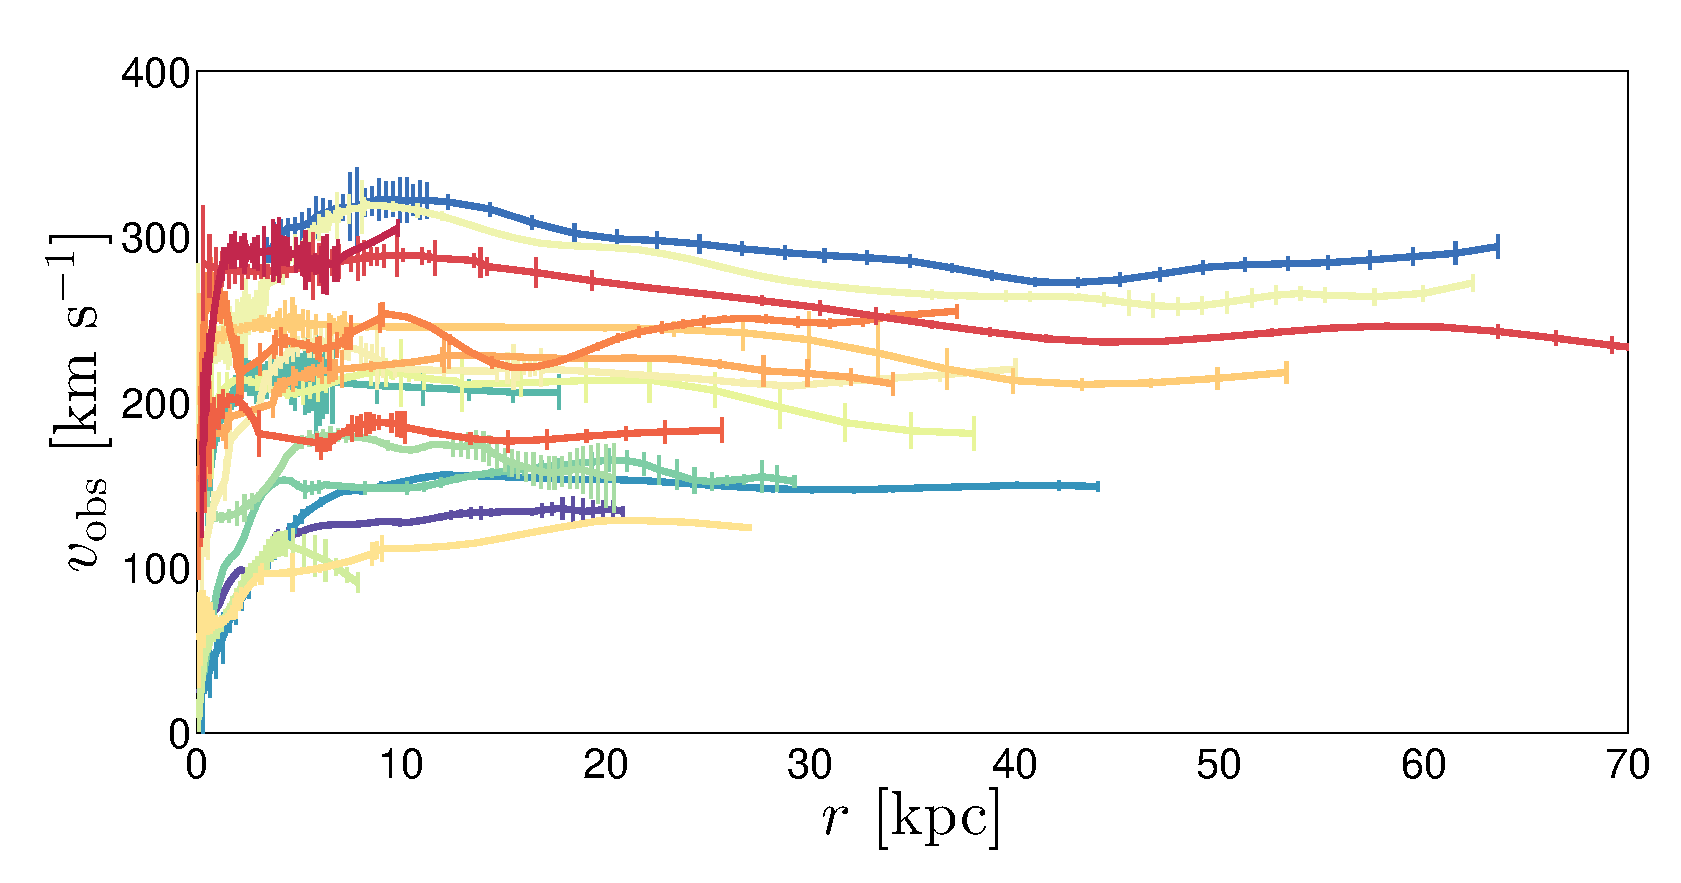
\includegraphics[width=\textwidth]{Figures/galrot.eps}
\caption[SPARC galaxy rotation curves]{Sample of disk galaxy rotation curves from SPARC. The rotation curves are shown as observed speed $v_{\rm obs}$, as a function of radius $r$. Despite the galaxy-to-galaxy differences there is consistent flattening at large $r$, contrary to the Keplerian prediction.}\label{fig:galrot}
\end{center}
\end{figure}

\subsection{Galaxy clusters}\label{sec:intro_galclusters}
Galaxy clusters contain 100~-~1000 galaxies of varied size and are the largest gravitationally bound structures in the Universe. They were also the first objects to have observations indicate the need for dark matter. Zwicky's 1933 observation of the Coma cluster showed a discrepancy of a factor of a few hundred between the luminous mass and the gravitational mass implied by the virial theorem~\cite{Zwicky:1933gu}. Since these early observations, many more sensitive probes of galaxy cluster masses have been developed. Gravitational lensing techniques involving the analysis of distorted images of distant galaxies due to the deep potential of clusters can be used as an independent measure of the total gravitational mass~\cite{Bartelmann:1999yn,Applegate:2012kr,Applegate:2015kua}. Strong gravitational lenses can also be used to weigh the masses of individual galaxies~\cite{Oguri:2013mxl}. Complementary to lensing, X-ray bremsstrahlung emission from the hot electron plasma (which typically comprises the majority of the mass of the baryonic component\footnote{We make use of the convention in cosmology to refer to all hadronic and leptonic matter as `baryons'.}) can be used to construct temperature profiles and subsequently an independent estimate of a cluster mass~\cite{Vikhlinin:2005mp,Ettori:2013tka,Ettori:2014wea,Tchernin:2015jda}. A combination of these observations with more sophisticated mass modelling and virial estimates~\cite{Carlberg:1995aq} together provide another overwhelming set of evidence for dark matter~\cite{Bryan:1997dn}. Furthermore there are individual cases of galaxy cluster collisions~\cite{Clowe:2006eq,Bradac:2008eu,Dawson:2011kf,Harvey:2015hha} (such as the archetype ``Bullet Cluster'' 1E0657-56~\cite{Markevitch:2003at}) which appear to show a striking separation between the luminous matter and a non-interacting dark component. Because galaxy clusters are the largest structures in the Universe it is not unreasonable to assume that they will be a good indicator of the contents of the Universe~\cite{Freedman:1997vk}. The evidence for dark matter from galaxy clusters and the evidence from rotation curves rely on independent measurements and probe length and mass scales many orders of magnitude apart, so when combined make a persuasive argument.

\subsection{Cosmology}\label{sec:intro_cosmology}
Galaxies aside, arguably the most compelling evidence for dark matter arrived with the advent of precision cosmology. The harbingers of this new era were satellites such as WMAP~\cite{Spergel:2003cb,Spergel:2006hy,Komatsu:2010fb} and subsequently Planck~\cite{Ade:2013zuv,Ade:2015xua} with measurements of the temperature anisotropies in the cosmic microwave background (CMB). Together with the rapidly expanding catalogues of large scale structure (LSS) from surveys such as SDSS~\cite{York:2000gk}, 2dF~\cite{Cole:2005sx}, DES~\cite{Abbott:2005bi} and CFHTLenS~\cite{Heymans:2012gg}, we now have an incredibly detailed view of the contents and evolution of the Universe on the largest scales and over the longest times.

The CMB is the ``first light'' of the Big Bang. It is a snapshot of the time of last scattering, when the Universe was around 380,000 years old. The release of photons occured when nuclei and electrons combined to form neutral atoms, making the Universe transparent for the first time. The spectrum of photons from the CMB form the most precise black body spectrum ever observed in nature with a temperature of 2.725~K~\cite{Fixsen:2009ug}. Despite this it has vitally important fluctuations in temperature across the sky with amplitudes $<~10^{-5}$~\cite{Smoot:1992td}, that may have originated from quantum fluctuations in a fundamental field driving a period of rapid inflated expansion~\cite{Guth:1980zm}. The gravitational collapse of the dark matter found in the subsequent overdensities and the infall of baryons into their potential wells, ultimately form the galaxies and clusters we see in the present day Universe. As well as temperature anisotropies across the sky the CMB photons have anisotropies in their polarisation, the distribution of which is also influenced by processes in the early and late Universe. Of particular note is the primordial B-mode polarisation which are a characteristic of gravitational waves produced generically in models of inflation~\cite{Ade:2014xna,Ade:2015lrj}.

Decomposing the distribution of CMB fluctuations as a function of angular scale, one can construct a power spectrum containing a series of peaks which encode the geometry, contents, and evolution of the early stages of the Universe. The peaks are formed due to acoustic oscillations in the photon-baryon fluid as the gravitational collapse of matter is resisted by the outward radiation pressure. Once this collapse has allowed structure to form, the CMB is imprinted upon again with an assortment of secondary anisotropies. As the CMB photons travel towards us they are blue- and redshifted by falling into and out of gravitational potentials (the Sachs-Wolfe effect~\cite{Giannantonio:2008zi}). The potential wells of galaxy clusters can also distort temperature and polarisation anisotropies on certain scales due to gravitational lensing. The spectrum of the CMB itself is also modified on very small angular scales by the Sunyaev-Zel'dovich (SZ) effect in galaxy clusters when photons are inverse Compton scattered by the hot electron plasma of the intra-cluster medium~\cite{Komatsu:2002wc}. Since the SZ effect is independent of redshift it can be used to count clusters out to large distances. The oscillatory behaviour of the photon-baryon fluid is also inscribed onto the power spectrum of the distribution of matter, meaning catalogues of large scale structure from galaxy surveys contain a valuable distance scale on the later Universe. In the context of LSS these are referred to as baryon acoustic oscillations (BAOs).

The most recent measurement of the angular power spectrum of the temperature and polarisation anisotropies of the CMB by Planck can be fit to good agreement by one of the simplest cosmological models in which the Universe is dominated by a cosmological constant $\Lambda$ and cold dark matter (CDM): the $\Lambda$CDM model. The cosmological constant is a uniform contribution to the energy density of the vacuum and is the simplest explanation for the apparent late time accelerated expansion of the Universe as indicated by the redshifts of type-1a supernovae~\cite{Riess:1998cb,Perlmutter:1998hx,Perlmutter:1998np}. 

To quantify the contents of the Universe we refer to the density of cosmological species as a fraction of the critical density (the density required for a flat Universe) $\Omega_i = \rho_i/\rho_c$, where $\rho_c = 3H_0^2/8\pi G$ in terms of the present day Hubble parameter $H_0$. When combined with complementary measurements from BAOs, weak lensing and type-1a supernovae, the Planck analysis find values of $\Omega_{\rm b} = 0.0486 \pm 0.0010$ and $\Omega_{\rm dm} = 0.2589 \pm 0.0057$ (when $H_0~=~67.74~\pm~0.46\,\,{\rm km\,s}^{-1}\,{\rm Mpc}^{-1}$~\cite{Ade:2015xua}) for the densities of baryons and cold dark matter respectively. In other words 84\% of matter is non-baryonic\footnote{Measurements of the densities of cosmological species are dependent on the square of present day Hubble parameter. Because of historical disagreement between local (e.g. Ref.~\cite{Riess:2016jrr}) and CMB measurements of $H_0$ it is usually expressed as the dimensionless $h~=~H_0/100\,\,{\rm km\,s}^{-1}\,{\rm Mpc}^{-1}$. In some cases we neglect to include $h$ to give an intuitive picture of an $\Omega_i$ as a fraction of the Universe's `energy budget'. In these cases we have inserted the local value mentioned above.}. This leaves the remainder of the energy budget of the Universe, $\Omega_\Lambda~\simeq~1-\Omega_{\rm b}~-~\Omega_{\rm dm}$ as the cosmological constant (since the Universe indeed appears to be flat~\cite{Komatsu:2010fb}, we have $\sum \Omega_i = 1$).

The need for dark matter is indicated from cosmological data alone simply due to the fact that baryonic density fraction is smaller than the total matter density fraction. The argument is made even more compelling still once these measurements are combined with an independent calculation known as Big Bang Nucleosynthesis (BBN). The calculation involves a solution to equations which govern the creation of the lightest nuclides ($^2$H, $^3$He, $^4$He and $^7$Li) during the first few minutes after the Big Bang and then matching the calculated abundances with observations~\cite{Alpher:1948ve,Yang:1983gn,Walker:1991ap}. Ultimately it is the ratio of baryons-to-photons ($n_b/n_\gamma~\sim~10^{-10}$) that dictates the resulting abundances and we can use this to infer the baryon density independently~\cite{Fields:2006ga,Fields:2014uja}. Updated BBN calculations that include uncertainties in measured abundances and nuclear rates set a range for the baryon density of $\Omega_{\rm b} = 0.048 - 0.052$~\cite{Ichimasa:2014fea} which is consistent with Planck and, crucially, smaller than the total matter density. The success of the standard BBN calculation - particularly the prediction of the abundance of deuterium - seems to disfavour the need for anything more exotic than CDM. Although the long-standing overestimate of the abundance of $^7$Li known as the `lithium problem' could be a hint towards the need for new physics (e.g. Ref.~\cite{Fields:2011zzb}).

\subsection{Simulations}
In the $\Lambda$CDM model while the cosmological constant is the dominant influence on the evolution of the Universe in the present day, we attribute the initial formation and growth of structure to cold dark matter. Baryons alone could not have formed large scale structure on the scales we see, or in a short enough time~\cite{Blumenthal:1984bp}. The processes through which overdensities collapse and form the distribution of structure is now well understood due to the success of large N-body simulations. In 2005, the Millenium simulation~\cite{Springel:2005nw}, the largest at the time, modelled the gravitational interactions of 2160$^3$ particles to track the evolution and growth of initial density perturbations in the early Universe. The results of these simulations, the network of sheets, links and filaments known as the cosmic web, show excellent agreement with the distribution of matter in wide surveys of galaxy redshifts~\cite{Cole:2005sx}.

Since then, advances in technology have allowed great improvements in the efficiency and accuracy of simulations on small scales and now include a variety of new physical processes involved with the inclusion of baryons. The most sophisticated projects such as the APOSTLE~\cite{Sawala:2015cdf,Oman:2016zjn} and EAGLE~\cite{Schaye:2014tpa} simulations, which trace the evolution of a small number of low-redshift Milky Way-like galaxies, are enriched with baryonic effects such as supernova feedback, stellar evolution and the physics of atomic and molecular gas. Hydrodynamic simulations can now self-consistently include the back reaction of baryons on dark matter and can trace the evolution of matter both inside galaxies and in the intergalactic medium. Importantly these simulations can have the level of baryonic interaction calibrated to match known relationships between different observables, such as the stellar or black hole masses of galaxies.

Simulations have now largely confirmed the central prediction of the cold dark matter paradigm: the assembly of structure by hierarchical merging of smaller halos to form larger ones~\cite{White:1977jf,Davis:1985rj,Kauffmann:1993jn,Kauffmann:1995gh}. Only a small number of notable problems remain (particularly in dark matter only N-body simulations), which relate to the internal structure of dark matter halos and subhalos. For instance the largest subhalos in simulations seem to be too dense to explain why the Milky Way's own largest satellites are so dim, so-called the `too big to fail' problem~\cite{BoylanKolchin:2011de}. There are also discrepancies between the cuspiness of the central density profiles of simulated satellite galaxies compared with the cored nature of their observed counterparts (the `core-cusp' problem~\cite{Moore:1994yx,Navarro:1996bv}). Lastly, the true abundance of satellite galaxies appears to be much smaller than predicted in simulations (the `missing satellite' problem~\cite{Klypin:1999uc}). Many of these problems have been alleviated either with a more careful treatment of baryonic feedback~\cite{Pontzen:2011ty,Governato:2012fa} or through more thorough and sensitive searches for fainter dwarf satellite galaxies~\cite{Simon:2007dq}. Alternatively they may be suggesting a need for the modification of $\Lambda$CDM as we will discuss shortly.

% Required properties of cdm

\section{Candidates for dark matter}\label{sec:intro_candidates}
The myriad pieces of evidence from astronomy and cosmology argue one of the best cases for particle physics outside of the standard model (SM). Devising sensible theoretical extensions to explain dark matter is an exciting challenge, but also a frustrated one given the success of the SM in explaining with remarkable accuracy the vast majority of experimental results. Dark matter especially presents a novel set of challenges as its known properties, though few in number, are supported by a wealth of precise observational evidence. In this Section we discuss some possible candidates for dark matter from a variety of different theoretical origins.

\subsection{Non-particle dark matter}\label{sec:intro_nonparticle}
While it is enticing to view the evidence for dark matter as an indication of new particles, we must first be sure that it cannot be explained with what we already know to exist. It was once believed that the missing mass in galaxies could consist of small dark objects formed through already understood astrophysical processes. If these were large and abundant enough to constitute a decent proportion of the halo but small enough and with low enough luminosity to evade detection, then they would be a natural solution to the missing mass problem. The umbrella term became `massive compact halo objects' (MACHOs) and would consist of a large, otherwise unaccounted for collection of faint stellar remnants, brown dwarfs, planets and other rocky debris. Now MACHOs have been ruled out as any sizable fraction of dark matter ~\cite{Freese:1999ge} by the absence of the microlensing events they would cause as they pass along lines of sight to nearby stars ~\cite{Tisserand:2006zx, Alcock:2000ph}. White dwarfs can also be independently excluded as a significant contribution to MACHOs because their formation in the required amounts would induce a much more chemically enriched intergalactic medium than observed~\cite{Fields:1999ar}. 

Another possibility is that dark matter is in the form of primordial black holes (PBHs) which are the relics of collapsed early Universe density perturbations~\cite{Carr:1974nx}. PBHs forming before BBN would be non-baryonic and an excellent dark matter candidate because in principle no new physics would need to be invoked to explain their existence\footnote{Unfortunately, based on existing constraints it is often not possible to produce enough PBH dark matter without some new physical mechanism involved with their formation~\cite{Carr:2016drx}.}. The abundance and masses of primordial black holes have been tightly constrained with microlensing searches~\cite{Tisserand:2006zx}, the dynamical heating dwarf galaxies~\cite{Brandt:2016aco}, the disruption of wide binary systems~\cite{Chaname:2003fn}, and the effect of Hawking radiation or accretion X-rays on the CMB~\cite{Clark:2016nst,Ricotti:2007au}. The attention on PBHs was reinvigorated in 2016 when the gravitational wave interferometry experiment LIGO made the first detection of gravitational waves due to the collision of two $\sim$10~$M_\odot$ black holes~\cite{Abbott:2016blz,Abbott:2016nmj}. The improbability of such a large event, based on existing star formation models, has drawn many to reconsider the possibility of PBHs in the same mass range~\cite{Bird:2016dcv,Sasaki:2016jop}. Despite the fact that $1 - 10^3\,M_\odot$ PBHs were excluded as a majority dark matter candidate by microlensing and dwarf galaxy dynamics, it was argued that the delta function mass spectrum assumed in placing these constraints was not appropriate for representing a population of PBHs left over from inflationary density perturbations~\cite{Kuhnel:2017pwq}. However a subsequent revision of these limits finds that no extended mass function can consistently explain both microlensing and dynamical constraints~\cite{Green:2016xgy}. It is hoped that upcoming observations of strongly lensed fast radio bursts will tightly constrain PBHs as a dark matter candidate in this mass range~\cite{Munoz:2016tmg}.

There have been long-standing efforts to attempt to explain the astrophysical evidence for dark matter with modifications to gravity. The best known example is Milgrom's Modified Newtonian Dynamics (MOND) where for very small accelerations the usual law of Newtonian gravitational attraction no longer applies~\cite{Milgrom:1983pn,Milgrom:1983ca,Milgrom:1983zz}. MOND has been successful in explaining the rotation curves of galaxies as it was designed to do~\cite{Sanders:1996ua}, but it has also seen recent success in explaining relationships between the baryonic and gravitational masses of galaxies. Empirical correlations such as the baryonic Tully-Fisher~\cite{McGaugh:2000sr,McGaugh:2011ac} and radial acceleration~\cite{McGaugh:2004aw,Lelli:2017vgz,McGaugh:2016leg} relationships are naturally explained in the context of MOND, and these recent results are in accordance with the initial predictions of Milgrom~\cite{Milgrom:2016uye}. It has also been shown that other modifications to gravity~\cite{Moffat:2016ikl} including screened fifth forces~\cite{Burrage:2016yjm} can recover the relationships. Such laws would not naively be expected from CDM, however it as also been argued that the effects of baryonic physics and the subsequent back reaction of dark matter during the formation of galactic disks explains why a connection between baryonic and gravitational masses occurs~\cite{Navarro:2016bfs,Sales:2016dmm}.

The difficulty in constructing a purely gravitational explanation for dark matter is that as well as explaining observations on a galaxy-to-galaxy basis, it is essential that MOND can emerge from a fully relativistic theory of gravity. In addition to simply recovering the remarkable successes of general relativity on Solar System scales, we also require a formalism for calculating cosmological perturbations and gravitational lensing. Bekenstein's Tensor-vector-scalar gravity (TeVeS) is a covariant generalisation that reproduces MOND in the weak field limit~\cite{Bekenstein:2004ne}. MOND and TeVeS are generally disfavoured as an explanation for dark matter principally because of limited success in explaining the diverse catalogue of evidence. Galaxy rotation curves are a simple testbed but a modified gravity must also self-consistently explain lensing data, the distribution of matter in colliding galaxy clusters and the power spectrum of large scale structure~\cite{Ferreras:2012fg,Mavromatos:2009xh,Ferreras:2009rv}. Most damningly however, the evidence for $\Omega_{\rm b} < \Omega_{\rm m}$ indicated by the CMB and BBN is particularly difficult to explain from this perspective when compared to $\Lambda$CDM~\cite{Slosar:2005fg}. 

% Anne disagrees about the core-cusp problem

\subsection{Neutrinos}\label{sec:intro_neutrinos}
As the evidence for dark matter was beginning to emerge, many believed that the unexplained extra mass in the Universe might be accounted for with neutrinos, the properties of which were (and still remain) largely mysterious. Neutrinos naively fit the bill in that they possess a small mass and certainly interact rarely enough for them to have evaded detection. We now believe however that neutrinos cannot make up even a significant amount of the dark matter for two main reasons. 

The first argument involves their cosmological abundance. Neutrinos were produced in the early Universe in thermal and chemical equilibrium with a bath of other standard model particles. As the Universe expands and cools the rate of interactions producing and destroying neutrinos slows. Eventually below a certain temperature the equilibrium of neutrino production cannot be maintained and the neutrinos will `freeze-out' with a certain abundance called the relic density. Neutrinos freeze-out at a temperature of $T \sim \mathcal{O}(1\,{\rm MeV})$ when the interaction rate $\Gamma_\nu(T)$ falls below the expansion rate given by the hubble parameter $H(T)$. The rate is proportional to the thermally averaged cross section $\langle \sigma_\nu v \rangle$ on the order the Fermi constant, $\sigma_\nu \sim G_F^2$. After freeze-out neutrinos essentially interact only gravitationally so the final relic density is given by the sum of the neutrino masses~\cite{Lesgourgues:2006nd},
\begin{equation}\label{eq:nudensity}
 \Omega_\nu h^2 = \frac{\sum_{i=1}^3 m_{\nu_i}}{93.14\,{\rm eV}} \, .
\end{equation}
Solar and atmospheric neutrino oscillation experiments can measure mass differences between two neutrino mass states from which it can be inferred that the sum of the neutrino masses must be larger than $\sum m_{\nu_i} > 0.06$~eV~\cite{GonzalezGarcia:2012sz}. An upper bound can also be estimated with tritium $\beta$-decay experiments to be around $\sim$6~eV~\cite{Drexlin:2013lha,Lesgourgues:2014zoa}. Hence the density of neutrinos in the Universe must be less than $\Omega_\nu \lesssim 0.14$ and are unlikely to be able to account for dark matter.

In fact, cosmological data has been used to set an even tighter upper limit on the sum of the neutrino masses. The constraint is made by extending the minimal $\Lambda$CDM model by promoting $\sum m_{\nu_i}$ to a seventh free parameter\footnote{Interestingly, cosmological bounds on neutrinos are becoming so stringent that they will soon be able distinguish between the normal and inverted ordering of their mass states~\cite{DeBernardis:2009di}.}. The most recent bound from a combination of Planck polarisation and temperature anisotropies with BAO data is $\sum m_{\nu_i} < 0.151$~eV~\cite{Vagnozzi:2017ovm}. Note that the fit assumes a population of massive neutrinos {\it in addition} to cold dark matter. These early Universe neutrinos make up a background of relics with a temperature slightly lower than the CMB and a present day density of around 300 cm$^{-3}$. Unfortunately with redshifted energies around $10^{-4}$~eV the detection prospects are slim~\cite{Betts:2013uya}.
 
The second and now most critical argument disfavouring neutrinos as a dark matter candidate is from the perspective of the distribution of large scale structure. As mentioned in the previous section cosmological data appears to be well fit by a Universe containing $\Lambda$ and {\it cold} dark matter. The distinction between hot versus cold dark matter is in whether the dark matter is produced relativistically or not. Neutrinos were widely discussed as a hot dark matter (HDM) candidate~\cite{Pogosian:1994ns} but were eventually excluded due to their disastrous effect on structure formation. The central problem is that the growth of structure from initial density perturbations is washed out below a certain scale due to the thermal motions of particles. This scale is set by the typical comoving distance over which particles travel over the age of the Universe and results in a cutoff in the power spectrum of matter at large wavenumbers~\cite{Frenk:2012ph}. This so-called free streaming length decreases with the mass of the particle $\lambda~\propto ~m^{-1}$ and for neutrinos (or any HDM) this cuts off structure below the size of a galaxy cluster. In a Universe in which neutrinos are dark matter the formation of galaxy sized halos is impossible. As such the cold dark matter paradigm - permitting structures much smaller than observed dwarf galaxies - has become the preferred cosmology.

It is worth briefly mentioning the intermediate case known as warm dark matter (WDM), for masses $m \sim 2$ keV when the free streaming length is roughly on the scale of a dwarf galaxy. There are some hints this may solve problems in comparisons between simulations and the observed structure of dark matter halos. WDM has been shown in the past to ease problems with the cores of dwarf galaxies~\cite{Boyanovsky:2007ay} or the `too big to fail' problem~\cite{Lovell:2016nkp}. Candidates for WDM are also theoretically motivated. An example, sterile neutrinos, are a heavier fourth species of neutrino that undergo oscillations but have no electroweak interactions~\cite{Dodelson:1993je,Kusenko:2006wa}. Sterile neutrinos appear in many extensions of the standard model such as seesaw mechanisms to explain the masses of the three `active' neutrinos~\cite{Abazajian:2012ys} and there have been suggestions that some experimental anomalies cannot be explained by the mixing of only three neutrinos~\cite{Aguilar-Arevalo:2013pmq,Aguilar:2001ty,Mention:2011rk,Adamson:2016jku}. Sterile neutrinos have also been shown to slightly alleviate tensions between CMB and LSS data~\cite{Battye:2013xqa,Battye:2014qga} and their decay has been invoked in explanations of unidentified X-ray emission lines~\cite{Boyarsky:2014jta,Bulbul:2014sua}. However it remains to be seen if these problems can all be resolved consistently with the same sterile neutrino or if there is a mechanism to produce them in the right amounts~\cite{Shakya:2015xnx}. Furthermore many of these problems can be explained by other means. 

\subsection{WIMPs}\label{sec:intro_WIMPs}
Cosmological data dictates that dark matter must be produced cold and collisionless with a relic density of $\Omega_{\rm dm} h^2 =  0.1188 \pm 0.0010$~\cite{Ade:2015xua}. We also know that it must be stable, at least over the time taken to affect the CMB and still be present in galaxy halos today. But given that we are yet without indication of the precise particle nature of dark matter we know that it must have interactions small enough with the remaining three forces for it to have not caused too much disruption to structure formation or otherwise unexplained excesses in radiation. For instance, dark matter with any significant electromagnetic charge ($>10^{-6}e$ for a 1 GeV mass dark matter particle for example) would heavily disrupt the formation of the acoustic peaks of the CMB~\cite{McDermott:2010pa}. Any other sizable interactions for instance via the strong force or to any electrically neutral particle would provide an additional mode of energy transfer between baryons and dark matter and and would generally slow galaxy formation. What remains allowed however is a general class of dark matter candidate: weakly interacting massive particles (WIMPs). WIMPs are heavy, stable, weakly coupled particles that are assumed to self annihilate. The WIMP dark matter hypothesis is famously motivated with an argument known as the `WIMP miracle'~\cite{Wolfram:1978gp,Srednicki:1988ce,Scherrer:1985zt,Gondolo:1990dk}. 

As we described previously, particles that are in thermal equilibrium of creation and annihilation during some early epoch undergo freeze-out. This occurs when the expansion and cooling of the Universe dilutes the particles to a density at which they are being produced at a rate slower than the expansion rate $H$. The interaction rate is given by the thermally averaged annihilation cross section $\Gamma = n_\chi \langle \sigma_{\rm ann} v \rangle$. The number density of particles in equilibrium with $g$ internal degrees of freedom can be defined~\cite{Jungman:1995df},
\begin{equation}
 n_\chi(t) = \frac{g}{(2\pi)^3} \int \textrm{d}^3 p \, f(E,t) \, ,
\end{equation}
where $p$ is momentum and $f(E,t)$ is the time dependent phase space distribution determined by the spin statistics of the particle i.e. bosonic or fermionic. As the Universe expands the evolution of the number density will evolve according to the Boltzmann equation,
\begin{equation}\label{eq:boltzmann}
 \frac{\textrm{d}n_\chi}{\textrm{d}t} + 3 H n_\chi = -\langle \sigma_{\rm ann} v \rangle \left[ n_\chi^2 - (n_\chi^{\rm eq})^2\right] .
\end{equation}
In which $n^{\rm eq}_\chi$ is the equilibrium number density of dark matter particles which follows a Maxwell-Boltzmann distribution,
\begin{equation}
n^{\rm eq}_\chi \sim \left\{
\begin{array}{llrr}
T^3 &	\ \text{for $T \gg m_\chi$\,}  \\
(m_\chi T)^{3/2} \exp(-m_\chi/T)	& 	\ \text{for $T \ll m_\chi$\,,} 
\end{array}\right.
\end{equation}
depending on the temperature $T$ relative to the WIMP mass $m_\chi$. We see then from Eq.~(\ref{eq:boltzmann}) that for temperatures where the reaction rate is larger than the Hubble rate $\Gamma> H$, the number density is maintained at $n_\chi^{\rm eq}$. However as the Universe inevitably expands, the temperature will drop and for low $T$ the number density becomes Boltzmann suppressed by the exponential factor. Eventually the Hubble expansion rate which falls with temperature more slowly, ($H \propto T^2$ during radiation domination for example) will eventually exceed $\Gamma$. When it does the average time per interaction becomes longer than the age of the Universe and WIMP annihilation and creation can no longer maintain equilibrium. At this point the WIMPs chemically decouple from the thermal bath and their number freezes out leaving a final population of dark matter relics for the remainder of cosmic time. The temperature of freeze-out $T_f$ can be found by setting $\Gamma(T_f) \sim H(T_f)$. The relic density then follows after solving the Boltzmann equation at the present day, with initial conditions $n_\chi^{\rm eq}(T_f)$ and the removal of the collisional term (i.e. Hubble dilution $\textrm{d}n_\chi/\textrm{d}t = -3 H n_\chi$). The final density parameter in terms of the thermally averaged annihilation cross section is~\cite{Wolfram:1978gp,Srednicki:1988ce,Scherrer:1985zt,Gondolo:1990dk}
\begin{equation}\label{eq:relicdensity}
 \Omega_{\rm dm} h^2 \simeq 0.1 \left(\frac{3 \times 10^{-26}\,\,\textrm{cm}^3\,\textrm{s}^{-1}}{\langle \sigma_{\rm ann} v\rangle}\right) \, .
\end{equation}
Expressing $\Omega_{\rm dm}$ in this form shows that the observed relic density of dark matter points to a canonical value for the thermally averaged cross section around the weak scale. This argument is rather general and in practice many additional physical effects must be taken into account in accurate calculations of the relic density, for instance we have neglected the dependence on the WIMP mass and variation in the number of degrees of freedom~\cite{Steigman:2012nb}. However the basic argument holds and provides compelling motivation for candidate particles interacting with the standard model via the weak sector. The `miraculous' element of the WIMP miracle is that the argument points to particles which are simultaneously one of the only generic classes consistent with observation. The hypothesis also implies its own testability using three independent and complementary detection strategies that we discuss in Sec.~\ref{sec:intro_detection}.

Secondary, but rather crucial motivation for WIMPs originates from their natural appearance in many beyond the standard model theoretical frameworks, most notably that of supersymmetry (SUSY)~\cite{Jungman:1995df}. Supersymmetry is a principle which may be added to the fundamental construction of the SM to posit a symmetry between matter and forces, i.e. between fermions and bosons. It was realised in the 1970s that the normal symmetries of the S-matrix of quantum field theories (Lorentz boosts, rotations and translations, as well as internal symmetries) could be extended with the inclusion of generators that convert between bosonic and fermionic states~\cite{Gervais:1971ji,Akulov:1974xz,Wess:1974tw}. A theory that obeys supersymmetry has bosonic and fermionic states paired with identical mass and quantum numbers except for a difference in spin of $1/2$~\footnote{Superpartners to standard model fermions are bosons called sfermions with the prefix `s'. Superpartners to the standard model gauge bosons are fermions called gauginos with the suffix `ino'.}. Since we cannot pair up the standard model like this and no evidence has been found for any new particles, if supersymmetry is a symmetry of nature it must be broken meaning the masses of the superpartner particles exist beyond the TeV scale. Broken or otherwise, supersymmetric models are important solutions to a number of existing problems, most notably the ``hierarchy problem".

It is well known that the calculation of the Higgs mass is drastically unstable and sensitive to any unknown physics that might exist in the gulf between the electroweak and the Planck scales. The quantum corrections received by the squared Higgs mass from for instance, the heavy quarks, turn out to be large and quadratically sensitive to the ultraviolet cutoff between these two scales used to regularise the loop integrals. This ultraviolet cutoff is the scale at which the standard model ceases to be valid and a good effective theory should desirably be insensitive to it. Unfortunately this scale may be anywhere between a few TeV and the Planck scale $>10^{19}$ GeV. So for the weak scale masses of the Higgs, the W and the Z to be maintained this ends up requiring fine tuning of up to 1 part in 10$^{34}$.  In general SUSY rescues the divergence because the corrections from all the fermionic/bosonic standard model particles are cancelled by their bosonic/fermionic superpartners and the Higgs mass is stabilised.

In many SUSY models, to ensure the stability of the proton the conservation of $R$-parity is enforced. $R$-parity is defined as
\begin{equation}
R = (-1)^{3B+L + 2S}\, ,
\end{equation}
for states with baryon number $B$, lepton number $L$ and spin $S$. This quantum number is +1 for standard model particles and -1 for their superpartners~\cite{Martin:1997ns}. If $R$-parity is conserved then the decays of any SUSY particle must contain odd numbers of other SUSY particles. This means that the lightest supersymmetric particle (LSP) is energetically required to be stable as there are no lighter SUSY particles to which it can decay. Such particles are excellent dark matter candidates, providing further motivation for SUSY. In many models the favoured LSP is the neutralino which is a mixed state consisting of a linear combination of the neutral -inos (the Higgsinos and neutral wino and bino). The lightest neutralino in the simplest realisation of supersymmetry, the minimal supersymmetric standard model (MSSM), has typically a $\sim$100~GeV~-~1~TeV mass~\cite{Jungman:1995df} and is a Majorana fermion so self-annihilates as required.

Other SUSY models such as the next to minimal supersymmetric model, constrained minimal supersymmetric model or minimal supergravity can predict other superpartners for the LSP and may give rise to other dark matter candidates: the gravitino, sneutrinos or axino for example. Moreover, alternative beyond-the-standard-model frameworks such as universal extra dimensions models can predict WIMP candidates~\cite{Hooper:2007qk}. For the remainder of this thesis however we consider only the generic WIMP and remain agnostic with regards to its deeper origin. 
% NEED REFS FOR ALL THESE MODELS

\subsection{Axions and axion-like particles}\label{sec:intro_axions}
Axions are light pseudoscalar particles that appear in the solution of Peccei and Quinn~\cite{Peccei:1977hh, Kim:2008hd} to explain the unnatural absence of CP-violation in quantum chromodynamics (QCD)\footnote{CP denotes the combination of charge conjugation and parity transformations which can either be conserved or violated in a theory.}. This strong CP problem as it is known arises because of an apparent need to fine tune a CP violating phase $\bar{\theta}$ to a value less than $10^{-14}$~\cite{Baker:2006ts} where in principle it could take any value from 0 to $2\pi$ with seemingly no anthropic preference. The Peccei-Quinn solution is to promote this phase to a field which is driven to 0 dynamically after the spontaneous breaking of a new U(1) symmetry. The mechanism predicts the existence of a new light pseudoscalar which was called the axion~\cite{Wilczek:1977pj,Weinberg:1977ma}\footnote{The axion was named after an American brand of laundry detergent by Wilczek since it was said to ``clean up" a problem with an ``axial'' current; narrowly missing out on the name ``Higglet'' as suggested by Weinberg~\cite{Wilczek:quantamag}.}. There are various models for how this symmetry breaking takes place that predict particular relationships between the axion mass and the strength of its couplings to the SM. The axion predicted in these models is referred to as the `QCD axion'. More recently, motivation from the landscape of axion-like particles (ALPs) appearing in string theory~\cite{Svrcek:2006yi,Arvanitaki:2009fg,Cicoli:2012sz} has inspired the generalisation of the QCD axion to light pseudoscalars originating outside of the original Peccei-Quinn solution. Such ALPs share phenomenology with the axion but can cover an extremely wide range of masses and couplings~\cite{Arias:2012az}.

Axions and ALPs are attractive cold dark matter candidates and it has been shown that they can be produced in the early Universe through a variety of non-thermal mechanisms such as vacuum misalignment or via the decay of topological defects~\cite{Davis:1986xc,Hiramatsu:2012gg} in ways that are consistent with the known cosmological abundance and phenomenology of CDM~\cite{Ipser:1983mw,Wantz:2009it,Marsh:2015xka}. Axions can be detected thanks to a coupling to electromagnetism which permits their conversion into photons. Certain mass and coupling ranges for ALPs can be ruled out with observations of astrophysical environments expected to produce them in significant quantites e.g. white dwarfs~\cite{Raffelt:1985nj,Isern:2008nt}, neutron stars~\cite{Berenji:2016jji}, red giants~\cite{Raffelt:1999tx} and supernovae~\cite{Burrows:1988ah,Mayle:1987as}. Axions may also be observable in the lab as we discuss in Sec.~\ref{sec:intro_axionexpts}.

\section{Detecting dark matter}\label{sec:intro_detection}
Despite the quantity of gravitationally based evidence, it is clear that the probes of dark matter that we have discussed so far are not sufficient to learn more about its particle nature. In this section we briefly summarise how dark matter may be detected in the future. WIMPs in particular have three principal detection strategies illustrated in Fig.~\ref{fig:detection-diag}. These are {\color{green}{direct detection}} in which WIMPs scatter off standard model targets, {\color{blue}{indirect detection}} in which WIMPs annihilate into standard model particles, and {\color{red}{production}} in colliders. We also discuss experimental searches for axions.

\begin{figure}[t]
\begin{center}
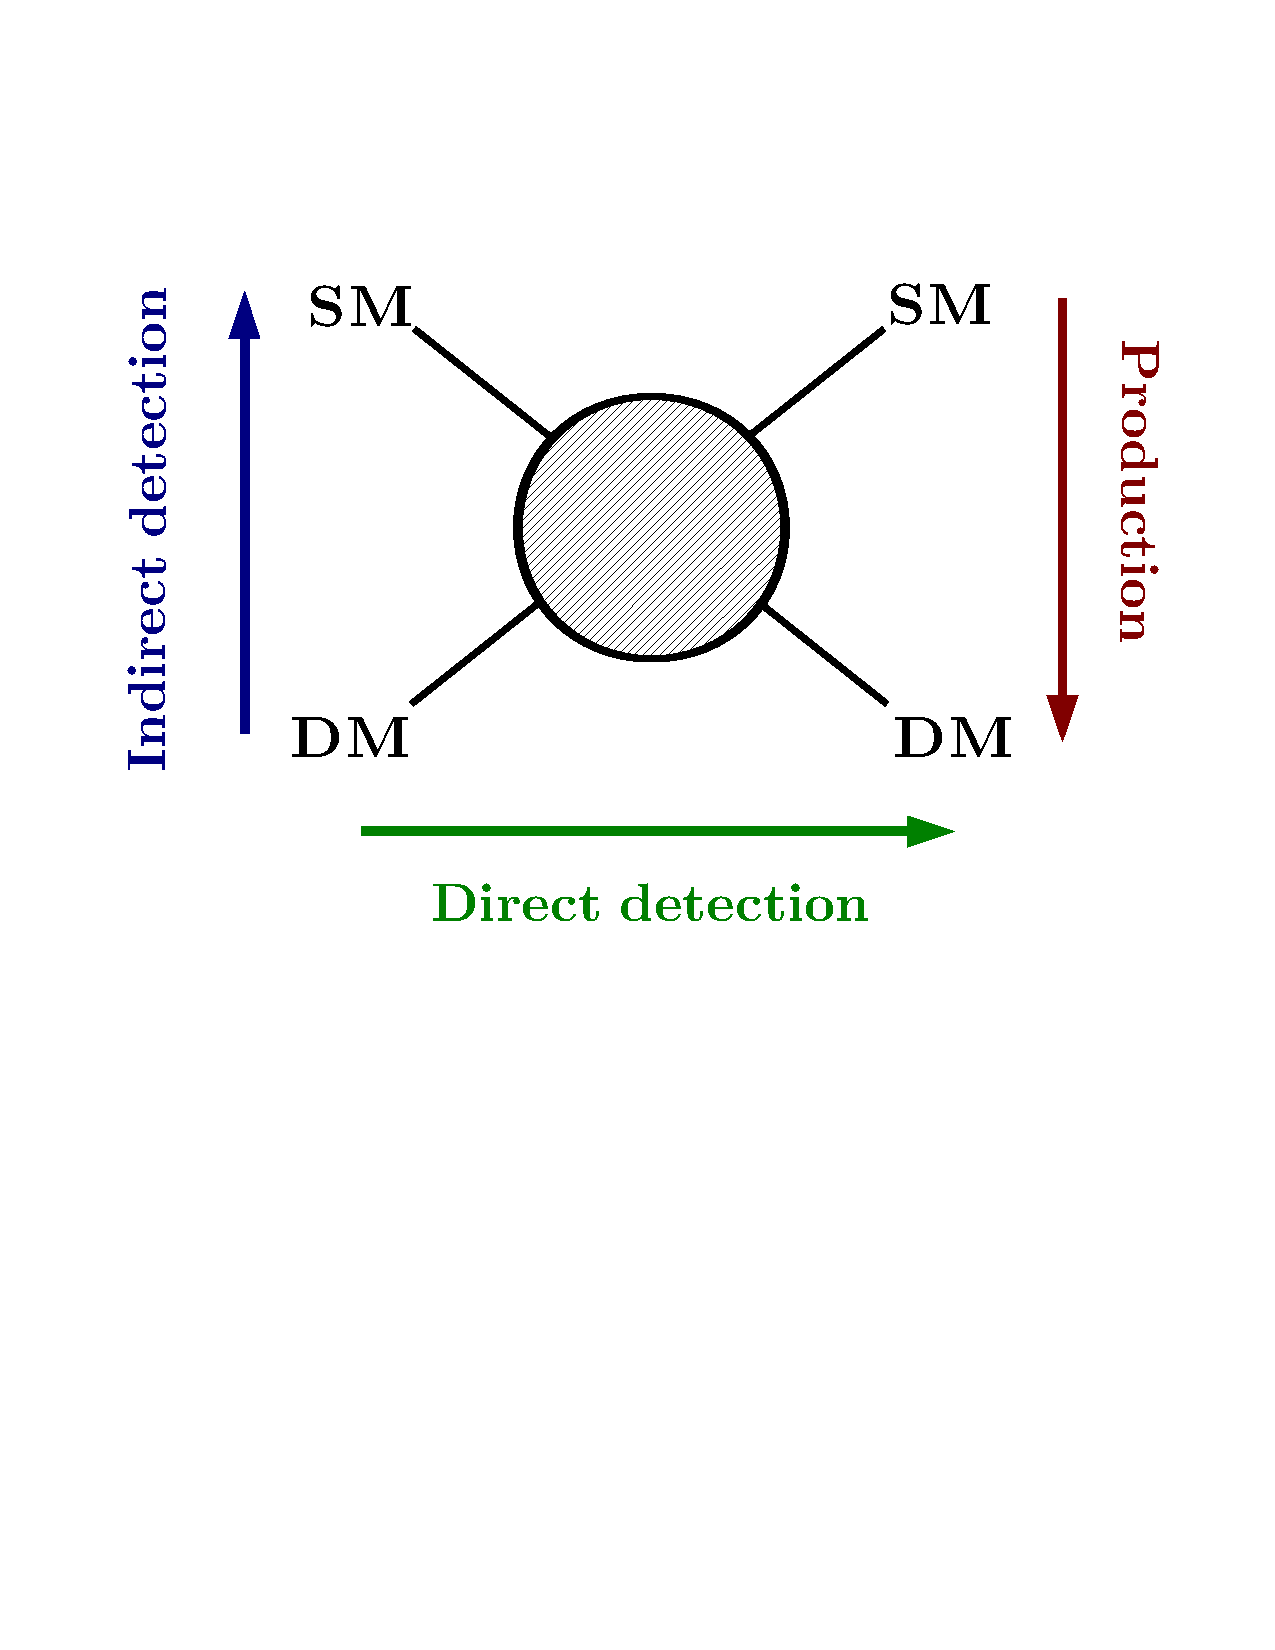
\includegraphics[width=0.7\textwidth,trim = 20mm 120mm 20mm 40mm,clip]{Figures/detection-diag.pdf}
\caption[Three strategies for detecting dark matter]{Diagram of the three principal strategies for detecting dark matter (DM) with standard model (SM) particles.}\label{fig:detection-diag}
\end{center}
\end{figure}

\subsection{Direct detection}\label{sec:intro_direct}
The Solar System is embedded inside a dark matter halo. Estimates from local astronomical data~\cite{Salucci:2010qr,Smith:2011fs,Bovy:2012tw,Garbari:2012ff,Zhang:2012rsb,Bovy:2013raa}, global comparisons with Milky Way mass models~\cite{Weber:2009pt,Catena:2009mf,Iocco:2011jz,Nesti:2013uwa,Sofue:2015xpa,Pato:2015dua} as well as simulations of Milky Way-like galaxies~\cite{Bozorgnia:2016ogo} all predict a non-zero density of dark matter at Earth with a value somewhere in the range $\rho_0 = 0.2 - 0.7$~GeV~cm$^{-3}$. We expect a flux of dark matter particles with speeds $\sim$200~km~s$^{-1}$ on Earth at all times. If WIMPs can scatter off standard model particles it should in principle be possible to see evidence of these interactions by searching for recoiling particles, usually nuclei~\cite{Goodman:1984dc,Drukier:1986tm}. The difficulty in designing a detector to search for these events is that there are a multitude of cosmic and terrestrial sources of background also inducing recoils in the expected keV energy scale. In addition to the steadily increasing physical size of these detectors the last few decades have seen continuous progress in background modelling, reducing energy thresholds and improving signal discrimination; all of which are necessary for pushing down the sensitivity to smaller cross sections and WIMP masses. The current most sensitive direct detection experiments, including LUX~\cite{Akerib:2013tjd}, Xenon100~\cite{Aprile:2011hx} and PandaX~\cite{Tan:2016zwf} have reached spin-independent WIMP-nucleon cross sections around $\sigma \sim  10^{-44}-10^{-46} \, {\rm cm}^2$.

The frontier of direct detection experiments is approaching the ton-scale in mass and near future experiments are expected to reach a sensitivity at which coherent scattering between nuclei and Solar neutrinos will begin to constitute a dominant background~\cite{Monroe:2007xp,Strigari:2009bq,Gutlein:2010tq,Billard:2013qya}. It is predicted that one of the upcoming ton-scale xenon experiments, LZ~\cite{Akerib:2015cja} or Xenon1T~\cite{Aprile:2015uzo}, will make the first measurement of coherent neutrino-nucleus scattering (CNS) due to $^8$B Solar neutrinos\footnote{CNS remains an unmeasured interaction of the standard model, though its cross section has been calculated~\cite{Freedman:1973yd}.}. Since they are impossible to shield, neutrinos are the ultimate background to direct detection. Because of the similarity between WIMP and neutrino recoil energy spectra in direct detection experiments, the large uncertainty in our knowledge of the neutrino flux imposes a lower limit on the discoverable WIMP-nucleon cross section called the neutrino floor~\cite{Billard:2013qya,Ruppin:2014bra,Davis:2014ama,Grothaus:2014hja,O'Hare:2015mda,OHare:2016pjy}.

It may be possible to distinguish neutrinos from WIMPs with the use of smoking gun Galactic dark matter signals. As well as measuring the energy of recoiling nuclei, direct detection experiments could in principle exploit time and direction dependencies. Due to the relative motion of the Earth and Sun with respect to the (largely non-rotating) dark matter halo, the peak flux of WIMPs should point back towards the constellation of Cygnus~\cite{Spergel:1999mh}. As the Earth revolves around the Sun we move with respect to this flux, thus annually modulating the recoil spectrum~\cite{Drukier:1986tm}. By the same argument there is also a very small daily modulation due to the rotation of the Earth~\cite{Bozorgnia:2011tk}. 

% evidence for non-rotating halo?

WIMP direct detection is the subject of Chapters~\ref{chapter:direct}-\ref{chapter:nufloor}. We begin with a detailed theoretical introduction and discussion of the experimental status in Chapter~\ref{chapter:direct}.

\subsection{Indirect detection}\label{sec:intro_indirect}
The annihilation of WIMPs was described in the context of the relic density calculation in the previous section. If WIMPs cluster in the Universe in regions of sufficiently high density then annihilation events may occur in sizable numbers. If the dark matter particle is heavy enough and its products energetic enough then it may be possible to detect them in a range of space and ground based cosmic ray detectors as well as neutrino telescopes. Detection or non-detection of excesses in for example the gamma ray flux from a region of suspected high dark matter density would provide a measurement or constraint on the annihilation cross section. The WIMP miracle suggests that this should be of the order $\langle \sigma_{\rm ann} v \rangle \sim 3 \times 10^{-26}$~cm$^3$~s$^{-1}$, Eq.~(\ref{eq:relicdensity}). 

The most important considerations for indirect searches are finding regions with large expected rates of annihilation that also have either low or well understood astrophysical emission. The proximity and high density of the Galactic center makes it an attractive place to search. Nearby dwarf spheroidal galaxies are also good targets as they are believed to be dark matter dominated with very low non-thermal gamma ray emission~\cite{Evans:2003sc,Fermi-LAT:2016uux}. A particularly desriable signal is a monoenergetic gamma ray line which could be emitted in certain final states. This would have no alternative standard astrophysical explanation and would be a smoking gun~\cite{Bergstrom:1994mg}, although continuum emission from hadronisation and decay of other products is expected to be larger. Predicting the gamma ray flux from annihilations requires first computing the line of sight integral of the square of the dark matter density towards the target (known as the $J$-factor). Then to extract a potential signal, all astrophysical background and foreground gamma ray emission must be modelled and subtracted. Through the non-observation of MW dwarf spheroidal galaxies, Fermi-LAT currently sets the tightest limits on the annihilation cross section~\cite{Ackermann:2015zua}. Of particular note however, an excess in the central 10$^\circ$ towards the Galactic center~\cite{Goodenough:2009gk,Hooper:2010mq} has had many claims put forward for a dark matter interpretation in the past (e.g. Refs.~\cite{Boehm:2014hva,Cahill-Rowley:2014ora,Cerdeno:2015ega,Caron:2015wda,Fonseca:2015rwa,Karwin:2016tsw}), however these can also be explained astrophysically with emission from a stellar overdensity~\cite{Macias:2016nev}, cosmic ray outbursts~\cite{Cholis:2015dea,Carlson:2016iis} or unresolved millisecond pulsars~\cite{Bartels:2015aea,Lee:2015fea,OLeary:2016cwz} for example. Furthermore, the most recent re-analysis by Fermi~\cite{TheFermi-LAT:2017vmf} has found similar sized excesses in other regions of the Galactic plane where no annihilation signal is expected. Going to larger energies than Fermi, due to the sharply decreasing gamma ray flux, larger effective areas are required. This makes ground based imaging atmospheric Cherenkov telescopes such as MAGIC~\cite{Doro:2017dqn}, HESS~\cite{Abdalla:2016olq}, VERITAS~\cite{Holder:2008ux}, HAWC~\cite{Proper:2015xya} (and in the future the Cherenkov Telescope Array (CTA)~\cite{Hofmann:2017lob}) more suitable.

Neutrino telescopes such as IceCube~\cite{Aartsen:2016pfc}, ANTARES~\cite{Collaboration:2011nsa}, Super-Kamiokande~\cite{Choi:2015ara} (and in the future Hyper-Kamiokande~\cite{Abe:2011ts}, PINGU~\cite{TheIceCube-Gen2:2016cap} and KM3NeT~\cite{Katz:2006wv}) are also useful for indirect searches since neutrinos, like gamma rays, point back towards their source and retain their spectral information. This is not true of charged cosmic rays which would also be produced in annihilations but propagate along complicated paths due to magnetic fields and have their spectrum softened by environmental processes. Antimatter cosmic rays are generally rare events however, so astrophysical backgrounds for positrons and antiprotons are inherently low. The trade off is in mapping the propagation of these particles through the Galaxy~\cite{Moskalenko:1997gh,Delahaye:2008ua,Strong:2004de}. PAMELA~\cite{Adriani:2008zr}, AMS-02~\cite{Aguilar:2013qda} and Fermi-LAT~\cite{FermiLAT:2011ab} have now all confirmed an unexpected rise in the positron to electron ratio from $\sim$10 to $\sim$100 GeV. As with other hints, both dark matter interpretations and astrophysical explanations have been suggested (e.g. Ref.~\cite{Fan:2010yq}). Analyses with antiprotons on the other hand are consistent with background models and currently set the best constraints among cosmic ray searches~\cite{Cuoco:2016eej}. The proposed experiment GAPS~\cite{Hailey:2009fpa} is hoped to be particularly powerful with its ability to detect antideuterons for which the astrophysical background is negligible~\cite{Donato:1999gy}.

\subsection{Colliders}\label{sec:intro_colliders}
WIMPs can be expected to be produced in high energy collisions performed in experiments at the Large Hadron Collider (LHC) such as ATLAS and CMS. Dark matter produced in collisions will not interact with the surrounding medium and are expected to stream out of the detector leaving remaining particles with large missing transverse momenta. Typically these are characteristic mono- signals such as -jets, -W, -Z, or -Higgs. ATLAS~\cite{Aad:2013oja,Aad:2015zva,ATLAS:2012ky,Aaboud:2017dor,Aaboud:2017yvp} and CMS~\cite{Khachatryan:2014rra,Khachatryan:2014rwa,Sirunyan:2017onm,Sirunyan:2017hnk,Sirunyan:2017hci} have both conducted searches for dark matter production in proton-proton collisions with a maximum center of mass energy of 13 TeV. To date there appears to be no evidence in significant conflict with the standard model, but constraints can be made. Ideally we would like these bounds to be expressed in the language of direct or indirect detection; in principle the three strategies should be highly complementary. Thankfully there exist frameworks for searching for general dark matter particles in LHC data. For instance the effective field theory approach (e.g.~\cite{Beltran:2010ww,Goodman:2010yf}) in which the SM-DM production is described as a contact interaction, or `simplified models' (e.g.~\cite{Buchmueller:2014yoa,Garny:2014waa,Liew:2016oon}) which are UV complete but introduce a SM-DM mediator that must also be constrained. However care must be taken as these frameworks carry assumptions which make the direct translation between interpretations of limits on dark matter a non-trivial process. 

Beyond technical considerations, a deeper issue with collider searches is that there is no way to demonstrate that a new particle is cold dark matter. Firstly a particle that streams out of the experiment may not be stable on a cosmological timescale. Secondly and possibly more worryingly is: how do we know if a new `dark' particle is the same as the one found in the Galaxy and beyond? Wheatever the case, any such signal will generate much excitement from the theoretical community\footnote{cf. over 500 arXiv submissions in 2016 about the now diminished diphoton excess at 750~GeV~\cite{750GeV}.} and if confirmed could point the way to more refined direct or indirect searches. 

\subsection{Other interactions}\label{sec:intro_other}
There exist other tests of dark matter interactions that do not fit neatly into this three pronged catagorisation. For example WIMP interactions in stars connect direct and indirect searches and can be used to probe both scattering and annihilation. It was realised some time before the advent of direct detection experiments that the Sun could act as a dark matter detector~\cite{Press:1985ug}. All stars embedded in the halo should sweep up a collection of dark matter particles as they orbit the galaxy. If a dark matter particle scatters off the Sun to a speed below the local escape velocity then it will become gravitationally trapped and left to orbit continuously around the Solar core~\cite{Gould:1987ir,Gould:1991hx}. Over time it is possible that stars could accumulate a high enough density for annihilations to occur. The only products that will be able to escape are neutrinos but these may be detectable on Earth~\cite{Silk:1985ax,Gaisser:1986ha,Srednicki:1986vj}. Observation or non-oberservation of high energy neutrinos from the Sun are another way to make constraints on the annihilation cross section~\cite{Choi:2015ara,Aartsen:2016zhm,Aartsen:2016exj} as well as a complementary way to probe scattering cross sections~\cite{Arina:2013jya,Kavanagh:2014rya}. Beyond our own Sun, in other stars such as white dwarfs annihilations would slow cooling and prolong lifetimes~\cite{Hurst:2014uda}, WIMP `burning' has also been suggested as a source of power for the first stars~\cite{Spolyar:2007qv,Freese:2015mta}.

% should mention cmb constraints 1512.08015 1310.3815	

It is also possible that dark matter interacts in slightly different ways and would not have a detectable signal using the strategies already discussed. For instance it may be that in high densities dark matter undergoes scattering self-interactions rather than annihilations. These observations would not have any direct observable signature in the form of products or decays. Instead self-interaction cross sections must be constrained by searching for distributions of dark matter that cannot be explained in terms of collisionless particles. Some of the small scale problems of N-body simulations, as described earlier, have been used to claim the need for these self interactions. In particular the cuspiness of the cores of simulated dwarf and low surface brightness galaxies could be resolved through heating and expansion via self-interaction~\cite{Spergel:1999mh, Rocha:2012jg, Zavala:2012us, Elbert:2014bma, Vogelsberger:2012ku, Fry:2015rta}, but these claims are in tight competition with constraints from colliding galaxy clusters~\cite{Harvey:2015hha, Randall:2007ph}. 

% what about claims from bullet cluster

\subsection{Axion experiments}\label{sec:intro_axionexpts}
The principal avenue to search for axions and ALPs is through their coupling to electromagnetism. In strong magnetic fields incoming axions can convert into a photon with energy approximately equal to the axion mass~\cite{Sikivie:1983ip}. How best to design an experiment to detect these photons depends on the source of the axions\footnote{We focus here on the coupling to photons but other couplings such as those to nuclei can be probed in nuclear magnetic resonance experiments such as CASPEr~\cite{Budker:2013hfa,Graham:2013gfa}. The axion coupling to electrons can also be constrained in WIMP direct detection experiments~\cite{Aprile:2014eoa,Akerib:2017uem}.}.

{\bf Dark matter axions} streaming in from the Milky Way halo will convert into photons inside magnetic fields in a lab setting although the power they produce will be extremely small. In a resonant magnetic cavity experiment however this axion conversion power is resonantly enhanced which can be achieved if the frequency of the cavity mode matches the axion mass. Since the mass is unknown, an experiment must be designed to scan over a range of resonant frequencies. This is achieved in the flagship `haloscope' ADMX with the use of movable tuning rods placed inside the cavity itself. There also exist alternative techniques with layered dielectric disks~\cite{TheMADMAXWorkingGroup:2016hpc} or dish antennae~\cite{Jaeckel:2015kea,Horns:2012jf}. Since haloscope experiments are the subject of Chapter~\ref{chapter:axions} we delay the full technical discussion until then.

{\bf Solar axions}: The Sun is expected to produce a flux of relativistic axions which can be detected in similar experiments called helioscopes. CAST looks for Solar axions converting into X-rays inside a long cavity pointed at the Sun over long exposure periods during the day~\cite{Zioutas:2004hi}. IAXO is a planned upgrade to CAST and will be able to constrain Solar axion couplings to even smaller values~\cite{Armengaud:2014gea}.

{\bf Laboratory axions}: It may be possible to produce axions in the lab and detect them in light-shining-through-a-wall experiments (LSW)~\cite{VanBibber:1987rq,Redondo:2010dp}. If light from a strong laser is passed through a magnetic field then photons could convert to axions and then back again on either side of an opaque barrier. Currently LSW experiments such as ALPS~\cite{Ehret:2007cm} are not sensitive enough to probe QCD scale axion couplings however the planned upgrade ALPS-II will improve upon the limits of its predecessor by three orders of magnitude~\cite{Bahre:2013ywa}.

It is important to emphasise the epistemological differences between these three experimental strategies. Haloscopes specifically look for dark matter axions/ALPs. Only if, for example ADMX, is successful in its search for axions will it confirm them as a dark matter candidate. If a helioscope or a future LSW experiment detects axions then this may confirm their role in the solution to the strong CP problem, but crucially it will {\it not} confirm them as a dark matter candidate. The other side of the coin to this is that Solar and laboratory experiments do not {\it require} axionic dark matter to detect axions.

\section{Summary}\label{sec:intro_summary}
% check
The success of the dark matter paradigm is borne out of both the quantity and precision of observational evidence but also the variety of that evidence. From sub-galactic scales up to the largest cosmological dataset, the evidence for the presence of dark matter is striking and one of the best arguments for physics beyond the standard model. In this introduction we have outlined two possible candidate classes of particle that are the subject of this thesis: weakly interacting massive particles, and axions. We have discussed their particle physics origin and methods of detection. This thesis will focus on the direct detection of axions and WIMPs, and in particular on future experiments and their potential to study those particles beyond simply identifying them. In particular we are interested in the uncertainty in the phase space structure of dark matter in the local Milky Way. Understanding these astrophysical uncertainties is important in achieving the particle physics goals of dark matter detection. On the other hand, as we will argue, terrestrial dark matter detectors are the only tools suitable for probing this astrophysical dependence.

This thesis is structured as follows. To begin, in Chapter~\ref{chapter:direct} we introduce the foundations for direct detection, deriving the WIMP-nucleus scattering event rate, discussing sources of particle and astrophysics uncertainty and outlining the current and future experimental effort. 

In Chapter~\ref{chapter:directional} we study the discovery reach of dark matter detection with directional sensitivity. We begin with a review of the key theoretical results and summary of the experimental techniques involved before showing how powerful these experiments are for constraining the astrophysical dependence of a dark matter signal. We first detail the particular case of tidal streams before considering general cases and the use of empirical methods for parameterising the velocity distribution.

In Chapter~\ref{chapter:nufloor} we consider future ton-scale experiments which are potentially sensitive to both WIMP and neutrino scattering. We first outline the calculation of the neutrino floor limit to direct detection and then show its dependence on various sources of uncertainty from the neutrino flux and dark matter astrophysical uncertainties. We then study methods of subtracting the neutrino background and potentially circumventing the floor. We briefly comment upon the use of timing information before studying in detail the most powerful method: directional detection. Here we consider a range of experimental uncertainties, in particular lower dimensional readout strategies. 

Finally in Chapter~\ref{chapter:axions} we move to axions. We first review the relevant particle physics motivation and summarise the existing constraints on the axion/ALP mass and coupling to photons. We then explore the potential for future microwave cavity experiments like ADMX to probe the phase space structure of the local dark matter halo. In analogy with the analysis presented in Chapter~\ref{chapter:directional} we devise a statistical technique to extract astrophysical information from simulated haloscope data and apply this to a range of cases including simple halo models, the Solar peculiar velocity, N-body simulation data and finally axion miniclusters.

The appendices contain expanded technical detail for: the laboratory velocity (\ref{app:labvelocity}), spherical statistics (\ref{app:dirstats}), a Monte Carlo scattering simulation (\ref{app:scattering}), the Solar vector (\ref{app:solar}), the profile likelihood ratio test (\ref{app:likelihood}), and expressions for some alternative speed distributions (\ref{app:fv}).

% Talk about target complementarity?
\chapter{WIMP Direct detection}\label{chapter:direct}
\lhead{\emph{WIMP Direct detection}}

In this Chapter we introduce the theoretical framework needed to predict signals in WIMP direct detection experiments. We begin in Sec.~\ref{sec:direct_WIMPnucleus} with the particle physics input: the WIMP-nucleus interaction and the derivation of the elastic scattering event rate. In Sec.~\ref{sec:direct_MW} we describe the astrophysical input including the local dark matter density and velocity distribution; we outline various sources of uncertainty and list the benchmark halo models used in later chapters. Then in Sec.~\ref{sec:direct_expts} we describe the experimental side of direct detection and summarise the existing constraints on the spin-independent (SI) and spin-dependent (SD) WIMP-nucleon elastic scattering cross sections.


\section{WIMP-nucleus interaction}\label{sec:direct_WIMPnucleus}

\subsection{Scattering rate}\label{sec:direct_rates}
We start with the calculation of the basic event rate expected in a detector placed on Earth. Since we are inside a dark matter halo we expect to be experiencing a flux, $\Phi_\chi$, of dark matter particles at all times. For a detector comprised of nuclei with mass $m_N$, the rate of collisions per unit detector mass will be proportional to the flux and some cross section, $\sigma$, describing the interaction coupling dark matter to the target,
\begin{equation}
 R = \frac{\Phi_\chi \sigma}{m_N} \, .
\end{equation}
We describe the rate of interactions in this way so as to generalise to experiments of arbitrary size and duration, this means that detector exposures must be quoted with dimensions of mass-time. The flux of dark matter particles we write in terms of the velocity distribution which for particles in velocity volume element $\textrm{d}^3 \textbf{v}$ is $\textrm{d}\Phi = n_\chi v f_\textrm{lab}(\textbf{v},t) \textrm{d}^3 \textbf{v}$, where $n_\chi$ is the DM number density. The time $de$pendent laboratory frame velocity distribution $f_\textrm{lab}(\textbf{v},t)$ is found by boosting the time $in$dependent Galactic frame  distribution by the velocity of the laboratory through the halo $\textbf{v}_\textrm{lab}$,
\begin{equation}
f_{\rm lab}({\bf v},t) =  f_{\rm gal}({\bf v} +{\bf v}_{\rm lab}(t)) \,.
\end{equation}
We can now express the event rate in terms of the velocity distribution. We can also introduce the WIMP mass and local DM density by writing the number density as $n_\chi = \rho_0/m_\chi$. 

Since direct detection experiments measure the energies of recoiling nuclei we would like to express the energy dependence of this rate by writing down $\textrm{d}R/\textrm{d}E_r$ by taking the derivative with recoil energy and then integrating over all WIMP velocities. However in doing this we must also enforce the kinematic constraint connecting the incoming WIMP speed, $v$, and the energy of the subsequent recoil,
\begin{equation}
 E_r = \frac{2 \mu^2_{\chi N} v^2}{m_N} \cos^2{\theta} \, ,
\end{equation}
which arises from simple momentum and energy conservation arguments. We have introduced the WIMP-nucleus reduced mass: $\mu_{\chi N} = m_\chi m_N / (m_\chi + m_N)$, and $\theta$ for the angle between the incoming WIMP velocity and recoiling nucleus. Since $m_N E_r/2\mu^2_{\chi N} v^2 \leq 1$ we have a minimum speed that can induce a recoil of energy $E_r$,
\begin{equation}
 \vmin = \sqrt{\frac{m_N E_r}{2 \mu_{\chi N}}} \, .
\end{equation}
We can now write the derivative of the rate with respect to energy but ensuring that we only integrate over WIMPs that are kinematically allowed to produce a recoil with $E_r$,
\begin{equation}
 \frac{\textrm{d}R(t)}{\textrm{d}E_r} = \frac{\rho_0}{m_N m_\chi} \int_{v>\vmin}^\infty v f(\textbf{v} + \textbf{v}_{\rm lab}(t)) \frac{\textrm{d}\sigma}{\textrm{d}E_r} \textrm{d}^3 \textbf{v} \, .
\end{equation}
This formula consists of particle physics inputs: the differential cross section and WIMP mass, and astrophysical inputs: the local DM density, velocity distribution, and time dependent lab velocity.

\subsection{Cross sections}\label{sec:direct_crosssections}
Differential WIMP-nucleus scattering cross sections, $\textrm{d}\sigma/\textrm{d}E_r$, are obtained through a low energy two particle scattering computation. A useful point at which to begin is with the formula for the derivative of the cross section with recoil energy expressed in terms of the matrix element $\mathcal{M}$ for the non-relativistic WIMP-nucleus scattering interaction,
\begin{equation}\label{eq:fermigoldenrule}
 \frac{\textrm{d}\sigma}{\textrm{d}E_r} = \frac{1}{32 \pi m_N m^2_\chi v^2} | \mathcal{M}|^2 \, .
\end{equation}
The matrix element is determined by a Lagrangian which describes the process through which the scattering takes place. We assume that the WIMP is a Dirac\footnote{For Majorana fermions the vector current, which is odd under charge conjugation, vanishes.} fermion $\chi$ and will have some interaction with quarks $q$. The Lagrangian could contain the following bilinear covariants describing possible exchanges between the WIMP and the quarks: $\chi$, $\bar{\chi}$, $q$, $\bar{q}$,
\begin{equation}\label{eq:lagrangians}
\mathcal{L}_q \sim
\begin{cases}
a^{\rm s}_q (\bar{\chi}\chi) (\bar{q}q) & \textrm{scalar}\\
a^{\rm v}_q (\bar{\chi} \gamma^\mu \chi) (\bar{q} \gamma_\mu  q) & \textrm{vector} \\
a^{\rm av}_q (\bar{\chi} \gamma^5 \gamma^\mu \chi) (\bar{q} \gamma^5 \gamma_\mu  q) & \textrm{axial-vector} \, ,\\
\end{cases}
\end{equation}
where $a^{\rm s}_q$, $a^{\rm v}_q$ and $a^{\rm av}_q$ are the corresponding couplings. It is commonplace to categorise these possible channels into those which are dependent on the spin of the nucleus and those which are not.

\textbf{Spin-independent (SI)} scattering occurs through scalar and vector interactions sourced by the exchange of, for example, the standard model Higgs or some heavy analogue to the Z boson. The scalar and vector currents give rise to cross sections that turn out to have the same functional form for Eq.~(\ref{eq:fermigoldenrule}). We present the calculation for the scalar interaction here. To evaluate the matrix element for the scattering with a nucleus via a scalar mediator we need to count up the contributions from the quark and gluon content in each proton and neutron. For ingoing (outgoing) states $|\psi_\chi\rangle$, $|\psi_N \rangle$ ($\langle \psi'_\chi|$, $\langle \psi'_N |$) we have the matrix element,
\begin{equation}
 \mathcal{M} = \langle \psi'_\chi| \bar{\chi}\chi | \psi_\chi \rangle \left( \langle \psi'_N | \sum_{\rm proton} a^{\rm s}_q \bar{q}q + \sum_{\rm neutron} a^{\rm s}_q \bar{q}q | \psi_N \rangle \right) \, .
\end{equation}
The first term can be simply calculated in the non-relativistic limit, for a Dirac fermion the expectation value of $\bar{\chi}\chi$ is just the spinor normalisation factor $2 m_\chi$. Calculating the second term is more involved since the scalar mediator will interact with not just the valence quarks but the sea quarks and gluons so the sums must count over all quark flavours and gluon fields. These contributions can be determined experimentally (their values are discussed in Ref.~\cite{Cerdeno:2010jj}, for example) but for our purposes it is more convenient to collect them into a coupling to protons $f_p$ and a coupling to neutrons $f_n$ which are defined as,
\begin{eqnarray}
 \langle \psi'_N | \sum_{\rm proton} a^{\rm s}_q \bar{q}q  | \psi_N \rangle &=& \langle \psi'_N | f_p \bar{p} p | \psi_N \rangle \, ,\\
 \langle \psi'_N | \sum_{\rm neutron} a^{\rm s}_q \bar{q}q | \psi_N \rangle &=& \langle \psi'_N | f_n \bar{n} n | \psi_N \rangle  \, .
\end{eqnarray}
Evaluating these two terms, the expectation value of $\bar{p} p$ and $\bar{n} n$ in the non-relativistic nuclear state $|\psi_N\rangle$ will then just give the number of protons or neutrons as well as a normalisation factor of $2m_N$. This results in the following for the matrix element,
\begin{equation}\label{eq:nuclearmatrixelement}
 \mathcal{M} = 4m_\chi m_N (f_p Z + f_n(A-Z)) F(E_r)\, ,
\end{equation}
for a nucleus with $A$ nucleons, $Z$ of which are protons. We have introduced the function $F(E_r)$ to parameterise the finite size of the nucleus which causes a loss in coherence in the nuclear scattering towards large momentum transfer. Inserting this matrix element into Eq.~(\ref{eq:fermigoldenrule}) we get,
\begin{equation}
 \frac{\textrm{d}\sigma}{\textrm{d}E_r} = \frac{m_N}{2\pi v^2} | f_p Z + f_n(A-Z)|^2 F^2(E_r) \, .
\end{equation}
We now change this formula slightly by substituting the total cross section found when scattering with just a proton $\sigma^{\rm SI}_p = \mu_{\chi p}^2 f_p^2 / \pi$ to get
\begin{equation}
 \frac{\textrm{d}\sigma_{\rm SI}}{\textrm{d}E_r} = \frac{m_N}{2\mu_{\chi p}^2 v^2} |Z + (f_n/f_p) (A-Z)|^2 \sigma^{\rm SI}_p F_{\rm SI}^2(E_r) \, ,
\end{equation}
where we now introduce the label `SI' to specify this is the cross section for spin-independent scattering. This change allows experiments to place constraints without needing to translate cross sections between different types of nuclei. The only model dependent choice we are required to make then is the ratio of the proton and neutron couplings. Most SI experimental limits are set under the assumption of equal couplings $f_n/f_p = 1$ which is true if WIMP scattering conserves isospin. In this case the nucleus enhances the event rate by a factor of $A^2$. From a theoretical perspective however one would not necessarily expect equal couplings, so this can be the source of some uncertainty when comparing exclusion limits.
 
\textbf{Spin-dependent (SD)} scattering takes place via an axial-vector interaction, for example in models where dark matter exchanges a SM Z boson with quarks. Now we must evaluate the matrix element,
\begin{equation}
 \mathcal{M} = \langle \psi'_\chi| \bar{\chi}\gamma^\mu \gamma^5 \chi | \psi_\chi \rangle \left( \langle \psi'_N | \sum_{\rm proton} a^{\rm av}_q \bar{q}\gamma_\mu \gamma^5 q + \sum_{\rm neutron} a^{\rm av}_q \bar{q} \gamma_\mu \gamma^5 q | \psi_N \rangle \right) \, .
\end{equation}
For a given nucleon, in the non-relativistic limit the matrix element for these operators is proportional to the product of the dark matter and nucleon spins $\propto 4 m_\chi m_n \textbf{s}_\chi \cdot \textbf{s}_N$. After averaging over the spin content of the nucleus, we have the result due to Engel~\cite{Engel:1992bf},
\begin{equation}\label{eq:sdcrosssection}
 \frac{\textrm{d}\sigma}{\textrm{d}E_r} = \frac{2 m_N}{\pi v^2} \frac{J+1}{J} | a_p \langle S_p \rangle + a_n \langle S_n \rangle |^2 F^2(E_r) \, ,
\end{equation}
where $J$ is the total nuclear spin, $a_p$ and $a_n$ are the WIMP couplings to the proton and neutron and $\langle S_p \rangle$ and $\langle S_n \rangle$ are the expectation values for the proton and neutron spins in the nucleus. As before, we insert the formula for the total SD proton cross section $\sigma_p^{\rm SD} = 3 \mu_{\chi p}^2 a_p^2 / \pi$ to arrive at, 
\begin{equation}
 \frac{\textrm{d} \sigma_{\rm SD}}{\textrm{d}E_r} =  \frac{2}{3} \frac{m_N}{\mu^2_{\chi p} v^2} \frac{J+1}{J} |\langle S_p \rangle + (a_n/a_p) \langle S_n \rangle |^2 \sigma^{\rm SD}_p F_{\rm SD}^2(E_r) \, .
\end{equation}
As with the SI case, to calculate this cross section we need to make a model dependent choice of $a_n/a_p$. Common choices are to assume either pure proton or pure neutron couplings (with constraints made on $\sigma^{\rm SD}_p$ or $\sigma^{\rm SD}_n$ appropriately) or specific relations such as $a_p/a_n = \pm 1$.

{\bf General event rate}: We can now write down a general formula for the elastic scattering rate on a target made of $n$ different {\it types} of nuclei with mass numbers $A^i = \{ A^1,...,A^n\}$,
\begin{equation}\label{eq:finaleventrate}
 \frac{\textrm{d}R(t)}{\textrm{d}E_r} = \sum_{i=1}^n \zeta^i \frac{\rho_0}{2\mu_{\chi p}^2 m_\chi} (\sigma^{\rm SI}_p \mathcal{C}^i_{\textrm{SI}} F^2_{\rm SI}(E_r) + \sigma^{\rm SD}_p \mathcal{C}^i_{\textrm{SD}} F^2_{\rm SD}(E_r))  \, g(\vmin,t) \, .
\end{equation}
where $\zeta^i = \{\zeta^{A^1},...\zeta^{A^n}\}$ are the fractions of the total number of nuclei in the detector made of a nucleus with $A^i$. In a single target material the $\zeta^i$ are interpreted as isotopic fractions whereas in a molecular or mixed target we must take into account isotopic fractions and the number of each type of nuclei in the molecule. In this formula we have absorbed all the dependence on the nuclear content into the form factors and an `enhancement factor', $\mathcal{C}^i_{\rm SI, SD}$, 
\begin{eqnarray}
 \mathcal{C}^i_{\rm SI} &=& | Z^i + (f_n/f_p)(A^i-Z^i)|^2 \, , \\
 \mathcal{C}^i_{\rm SD} &=& \frac{4}{3} \frac{J^i+1}{J^i} | \langle S_p \rangle^i + (a_n/a_p) \langle S_n \rangle^i |^2 \, .
\end{eqnarray}
We collect the dependence on the velocity distribution into $g(\vmin,t)$ which physically is the mean inverse speed greater than $\vmin$,
\begin{equation}\label{eq:gvmin}
g(v_{\rm min},t) = \int_{v>\vmin}^\infty \frac{f(\textbf{v}+\textbf{v}_\textrm{lab}(t))}{v} \, \textrm{d}^3 v \, .
\end{equation}
It should be noted that this is also a function of $E_r$ via $\vmin$.

The free parameters that we will use to describe the WIMP are its two cross sections with the proton $\sigma^{\rm SI,SD}_p$ and its mass $m_\chi$. We will assume that one of either SI or SD scattering dominates. As mentioned earlier, simplifying to just these parameters requires making a model dependent choice of the ratios of the proton and neutron couplings. In all of the following results we will make use of equal SI couplings to the proton and neutron $f_p/f_n = 1$ and for spin-dependent couplings we assume $a_n/a_p = -1$. We emphasise however that the results we present are not heavily influenced by these choices of coupling ratios. Different choices would only induce simple shifts in the total cross section and for SD interactions slight differences in form factors (see Sec.~\ref{sec:formfactors}). All of the following results will involve either or both of two example targets: fluorine and xenon. The spin contents and isotopic fractions of these two targets are displayed in Table~\ref{tab:nuclear} as well as a selection of other nuclei.

\begin{table}[t]\centering
\begin{tabularx}{\textwidth}{c|YYYYYY}
\hline \hline
		& $A$ & $Z$ & $J$& $\langle S_p \rangle$	& $\langle S_n \rangle$ & $\zeta$ \\
\hline
$^{19}\mathrm{F}$ & 19 & 9 & 1/2	& 0.421		& 0.045 	& 1 \\
$^{129}\mathrm{Xe}$ & 129 & 54	& 1/2	& 0.046 	& 0.293 	& 0.265\\
$^{131}\mathrm{Xe}$ & 131 &	54 & 3/2	& -0.038	& -0.242 	& 0.212\\
\hline
$^{73}\mathrm{Ge}$ & 73 & 32 & 9/2	&  0.030	& 0.378		& 0.0776\\
$^{29}\mathrm{Si}$ 	& 29 & 14 & 1/2	& -0.002	& 0.130 	& 0.0468\\
$^{127}\mathrm{I}$ & 127&	53 & 5/2	& -0.309	& 0.075		& 1\\
\hline \hline
\end{tabularx}
\caption[Nucleon numbers, spin content and abundances for various targets]{Nucleon content, proton and neutron spin averages, and isotopic abundances for nuclei with overall spin. The first three rows correspond to the nuclei considered in the remainder of this thesis whereas the following three rows are only those nuclei used for illustrative purposes in this Chapter. For spin contents of xenon and fluorine we use the two body corrections reported by Ref.~\cite{Menendez:2012tm} and Ref.~\cite{Cannoni:2012jq} respectively. For the remaining nuclei we use values from Ref.~\cite{Tovey:2000mm}.}
\label{tab:nuclear}
\end{table}
 
Although we consider only conventional SI and SD scattering here it is possible that dark matter interacts in a slightly more complicated way. Inelastic dark matter models with additional higher or lower excited states~\cite{TuckerSmith:2001hy, TuckerSmith:2004jv, Chang:2008gd, Bozorgnia:2013hsa, Blennow:2015hzp} have been introduced in the past to allow models to escape direct detection exclusion limits \cite{Fox:2013pia} and resolve tensions between various detection claims~\cite{Schwetz:2011xm}. Dark matter possessing both self interactions and excited states have been suggested as a solution to small scale structure formation problems \cite{Blennow:2016gde}. In asymmetric dark matter models~\cite{Kaplan:2009ag} the DM particle is charged under the baryon-lepton number asymmetry, B-L, responsible for the abundance of matter over antimatter in the Universe. Asymmetric models may lead to the existence of dark composite particles in analogy with hadronic matter, e.g. WIMPonium or `dark atoms' ~\cite{MarchRussell:2008tu, Pospelov:2008jd, Shepherd:2009sa, Laha:2013gva, Hardy:2014mqa, Laha:2015yoa}. These would be detectable in direct detection experiments but would require ton-scale detectors to distinguish their signal from a WIMP scenario~\cite{Butcher:2016hic}. We have also neglected the additional operators from the non-relativistic effective field theory framework. These were suggested in Ref.~\cite{Fan:2010gt} and subsequently developed in Ref.~\cite{Fitzpatrick:2012ix}. The operators generalise the DM-quark interaction beyond the three bilinear covariants listed in Eq.~(\ref{eq:lagrangians}) to include all Hermitian, Galilean and rotationally invariant combinations of the dark matter and nuclear spins, recoil momentum and incoming velocities. Some operators have been shown to have unique directional signatures~\cite{Kavanagh:2015jma} and have associated with them weakened neutrino floors~\cite{Dent:2016iht}. 
 
\subsection{Form factors}\label{sec:formfactors}
In Eq.~(\ref{eq:nuclearmatrixelement}) we introduced the form factor, $F(E_r)$, to describe how the spatial extent of the nucleus causes a loss in coherence in the interaction towards large momentum transfers. The form factor is defined as the deviation away from the zero momentum transfer limit, so $F(0) = 1$, which then decreases towards larger recoil energies. This decrease is steeper for heavier, more spatially extended nuclei because the loss in coherence takes effect at larger wavelengths than for lighter nuclei.

For SI interactions the form factor is, to a good approximation, the Fourier transform of the nuclear density distribution. This can either be calculated or extracted from data. Muon spectroscopy experiments have been often used in the past to extract parameters for SI form factors~\cite{Fricke:1995zz}. A commonly used $F_{\rm SI}(E_r)$ is the Helm ansatz~\cite{Helm:1956zz},
\begin{equation}
 F(E_r) = \frac{3 j_1(q r_1)}{(q r_1)^3} e^{-q^2 s^2} \, ,
\end{equation}
where $j_1(x) = (\sin{x} - x\cos{x})/x^2$ is a spherical bessel function of the first kind, $q~=~\sqrt{2 m_N E_r}$ is the recoil momentum and the exponential decrease is set by a nuclear skin thickness $s = 0.9$~fm. The radius of the nucleus, $r_1$, is commonly found using the formula,
\begin{equation}\label{eq:nuclearradius}
 r_1 = \sqrt{c^2 + \frac{7}{3} \pi^2 a^2 - 5 s^2} \, ,
\end{equation}
where $c = (1.23 A^{1/3} - 0.6)$~fm and $a = 0.52$~fm. The Helm ansatz is often used due to its simple analytic expression, however the density distributions of various nuclei extracted from muon spectroscopy data use a two-parameter Fermi assumption which does not have an analytic expression. The resolution introduced by Lewin and Smith~\cite{Lewin:1995rx} is to map the nuclear radius found in the two-parameter Fermi distribution into the Helm form of Eq.~(\ref{eq:nuclearradius}). This also involves the fixing of $s = 0.9$~fm by hand to improve the comparison. Though this is an {\it ad~hoc} comparison, more recent data and state of the art calculations have shown that for the energy scales probed by direct detection, the Helm form factor is a good approximation~\cite{Vietze:2014vsa,Co:2012adt} and is the one we will adopt. The form factor becomes important for heavy targets and high energy recoils from scattering with WIMP masses beyond $\sim$100 GeV. Since the majority of the results presented here will be for masses $<50$~GeV the form factor is a mostly subdominant consideration.

Determining SD form factors generally requires more computation and will in fact include the WIMP couplings to protons and neutrons $a_p$ and $a_n$ explicitly. In the isospin representation the couplings used instead are the isoscalar $a_0 = a_p+a_n$ and isovector $a_1 = a_p-a_n$, with the form factor written as $F^2(E_r) = S(E_r)/S(0)$, where $S(E_r)$ consists of a series of structure functions,
\begin{equation}
 S(E_r) = a_0^2 S_{00}(E_r) + a_1 a_0 S_{01}(E_r) + a_1^2 S_{11}(E_r) \, .
\end{equation}
This is the format usually adopted in nuclear physics calculations. The zero momentum limit used to rescale the structure function is written in terms of the spin content,
\begin{equation}
 S(0) = \frac{2J+1}{\pi}\frac{J+1}{J} | a_p \langle S_p \rangle + a_n \langle S_n \rangle |^2 \, .
\end{equation}
This means that the spin dependent cross section can be rewritten as,
\begin{equation}
 \frac{\textrm{d}\sigma_{\rm SD}}{\textrm{d}E_r} = \frac{2 \pi}{3} \frac{m_N \sigma^{\rm SD}_p}{\mu^2_{\chi p} v^2 (2J+1)} \frac{S(E_r)}{a_p^2} \, .
\end{equation}
Note that this equation differs from the simplified description introduced earlier in terms of $\mathcal{C}_N$, however we can recover Eq.~(\ref{eq:sdcrosssection}) once a specific nucleus and set of coupling values are chosen. In the following results involving SD interactions we use the recent calculation from Menendez {\it et al}.~\cite{Menendez:2012tm} for xenon, who absorb two-body corrections into the values of the spin content. For fluorine, we use the Divari {\it et al}.~structure functions \cite{Divari2000}, including the two-body nucleon corrections as reported by Cannoni \cite{Cannoni:2012jq}. In Fig.~\ref{fig:FormFactors} we show these SI and SD squared form factors for fluorine and the two xenon isotopes we use as targets.
\begin{figure}
\begin{center}
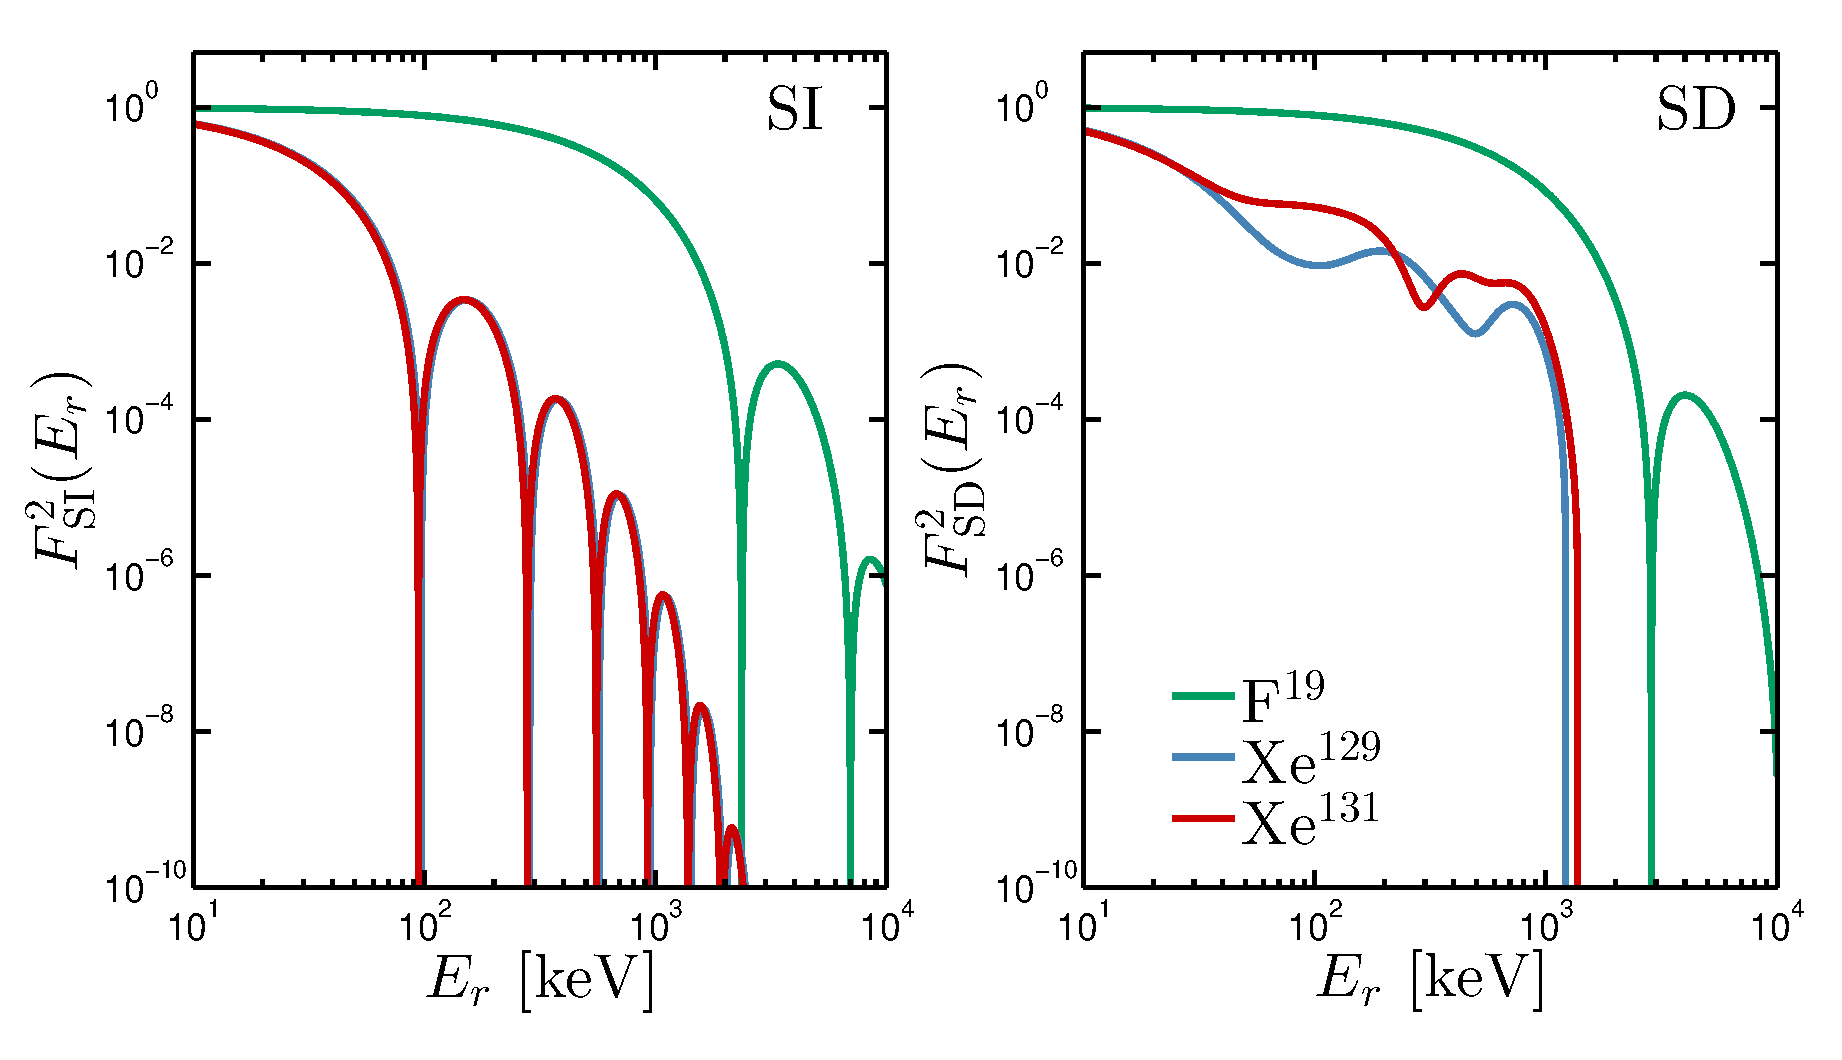
\includegraphics[width=0.97\textwidth]{Figures/FormFactors.eps}
\caption[Fluorine and xenon form factors]{Squared form factors for $^{19}$F (green), $^{129}$Xe (blue) and $^{131}$Xe (red) for spin-independent (left) and spin-dependent (right) interactions.}\label{fig:FormFactors}
\end{center}
\end{figure}

\subsection{Detector effects}
The goal of a direct detection experiment is to measure $\textrm{d}R(t)/\textrm{d}E_r$ in some way. The way this is achieved depends on the technology of the experiment as we will discuss in Sec.~\ref{sec:direct_expts}, however we can first define several key detector effects that modify the observed event rate. One of the most important detector effects to consider is the threshold energy $E_{\rm th}$. Experiments cannot observe arbitrarily small energies, meaning that all analyses will take place using recoils that have been observed above a given threshold. This energy may be a facet of the detector itself in cases where energies must be large enough to yield a detectable signal. The threshold energy is also sometimes enforced during data analysis, for example if there are large backgrounds or background uncertainties at low energies. Because $\textrm{d}R/\textrm{d}E_r$ drops exponentially with energy, achieving low $E_\textrm{th}$ has a big payoff in the total event rate so widening the signal acceptance to lower energies is a central goal of direct detection experiments in general. Lower thresholds are also of course required to access smaller WIMP masses. As well as a lower limit, we will also define a maximum cutoff energy, $E_\textrm{max}$, which is imposed in some experiments to deal with higher energy backgrounds or as the boundary of a signal acceptance region.

Real detectors will not be able to perfectly reconstruct the energy of a recoil. This is normally parameterised in terms of an energy resolution $\sigma(E_r)$ which must be taken into account when predicting the recoil energy spectrum that would be observed in an experiment. Extracting signals from a scattering event may also not be consistently efficient at all energies. This is accounted for in terms of an efficiency function $\epsilon(E_r)$ which typically drops off towards the threshold of the experiment. We define the `detector' recoil spectrum as a modification of the true recoil spectrum in the following way,
\begin{equation}
 \frac{\textrm{d}R_{\rm det}(t)}{\textrm{d}E_r} = \epsilon (E_r) \int_0^\infty K(E_r,E'_r)\frac{\textrm{d}R(t)}{\textrm{d}E'_r} \textrm{d} E'_r
\end{equation}
where $K(E_r,E'_r)$ is a Gaussian smoothing kernel,
\begin{equation}
K(E_r,E'_r) = \frac{1}{\sqrt{2\pi}\sigma(E_r)}e^{-\frac{(E_r-E_r')^2}{2\sigma^2(E_r)}} \, ,
\end{equation}
for an energy dependent resolution $\sigma(E_r)$. Most experiments will have some conversion factors that translate the signals observed in the detector into a recoil energy in keV and accounting for effects like quenching. We neglect these and their corresponding uncertainties as they will be very experiment specific. We also assume that our simulated experiments can achieve perfect discrimination between electron and nuclear recoils, meaning our mock data will consist solely of the latter. 

The total number of events seen in an experiment is controlled by both the physical size of the detector (i.e. its total mass $M$) and the running time $\Delta t = t_f-t_i$. This is usually expressed as an exposure with dimensions of mass-time. Including the aforementioned experimental factors this finally leaves us with a formula for the number of WIMP events to expect in a real experiment,
\begin{equation}
N_\textrm{WIMP} = M \int_{t_i}^{t_f} \int_{E_{\rm th}}^{E_{\rm max}} \frac{\textrm{d}R_{\rm det}(t)}{\textrm{d}E_r} \, \textrm{d}E_r \, \textrm{d}t \, . 
\end{equation}


\section{WIMPs in the Milky Way}\label{sec:direct_MW}
Predictions for signals in direct detection experiments require not only the description of the interaction between the dark matter particle and the target nuclei but also how those particles are phase space distributed in the region of the Milky Way around the Solar System. As introduced in the previous Section the key aspects are the local density, the velocity distribution and the velocity of the Earth through the halo which boosts the distribution into the laboratory frame. Since a dominant component of this thesis is involved with the astrophysics dependence we will now describe each of these in turn and their various sources of uncertainty.

\subsection{Local density}\label{sec:direct_density}
The local density of WIMPs, $\rho_0$, appears in Eq.~(\ref{eq:finaleventrate}) as a multiplicative factor. Since it shares this role with the interaction cross section, we require external knowledge of $\rho_0$ to break the degeneracy as we would not be able to constrain $\sigma$ otherwise. Measurements of the dark matter density are classed as either `local' or `global'. Local measurements are made by estimating the shape of the gravitational potential in the nearby Milky Way. This requires surveys of the vertical motions of nearby stars. There have been many determinations of $\rho_0$ made using this technique in the past dating back to the measurements of Kapteyn \etal~in the 1920s and 30s, see e.g. Refs.~\cite{Salucci:2010qr,Smith:2011fs,Bovy:2012tw,Garbari:2012ff,Zhang:2012rsb,Bovy:2013raa}. Global measurements on the other hand require first building a mass model for the Milky Way halo and then using tracers of the dynamics of the halo, such as the rotation curve, to fit the parameters of the model and subsequently infer the density at the Earth's Galactic radius. Measurements of this kind, e.g. Refs.~\cite{Weber:2009pt,Catena:2009mf,Iocco:2011jz,Nesti:2013uwa,Sofue:2015xpa,Pato:2015dua}, typically have larger systematic uncertainties than local determinations.

Estimates of $\rho_0$ have been historically variable with global measurements generally favouring slightly larger values. Recently however the two methods have started to converge~\cite{Bovy:2013raa,Piffl:2014mfa}.  Recent high precision surveys such as Gaia~\cite{Bailer-Jones:2013saa} will allow future measurements with small statistical uncertainties. However systematic modelling uncertainties will still be the dominant source of error, so methods for extracting the local density that rely on small numbers of assumptions will become essential~\cite{Silverwood:2015hxa}. The canonical value used by experiments is $\rho_0 = 0.3$~GeV~cm$^{-3}$ which we will also use to avoid unnecessary translation issues between our results and experimental limits. In the event of a positive WIMP signal an accurate value for the local density will be important for allowing an unbiased measurement of the cross section to relate to SUSY models, for example. However as many of our results are comparative in nature the precise value is not of huge importance, provided there is consistency. 

\subsection{Laboratory velocity}\label{sec:direct_vlab}
\begin{figure}
	%trim option's parameter order: left bottom right top
	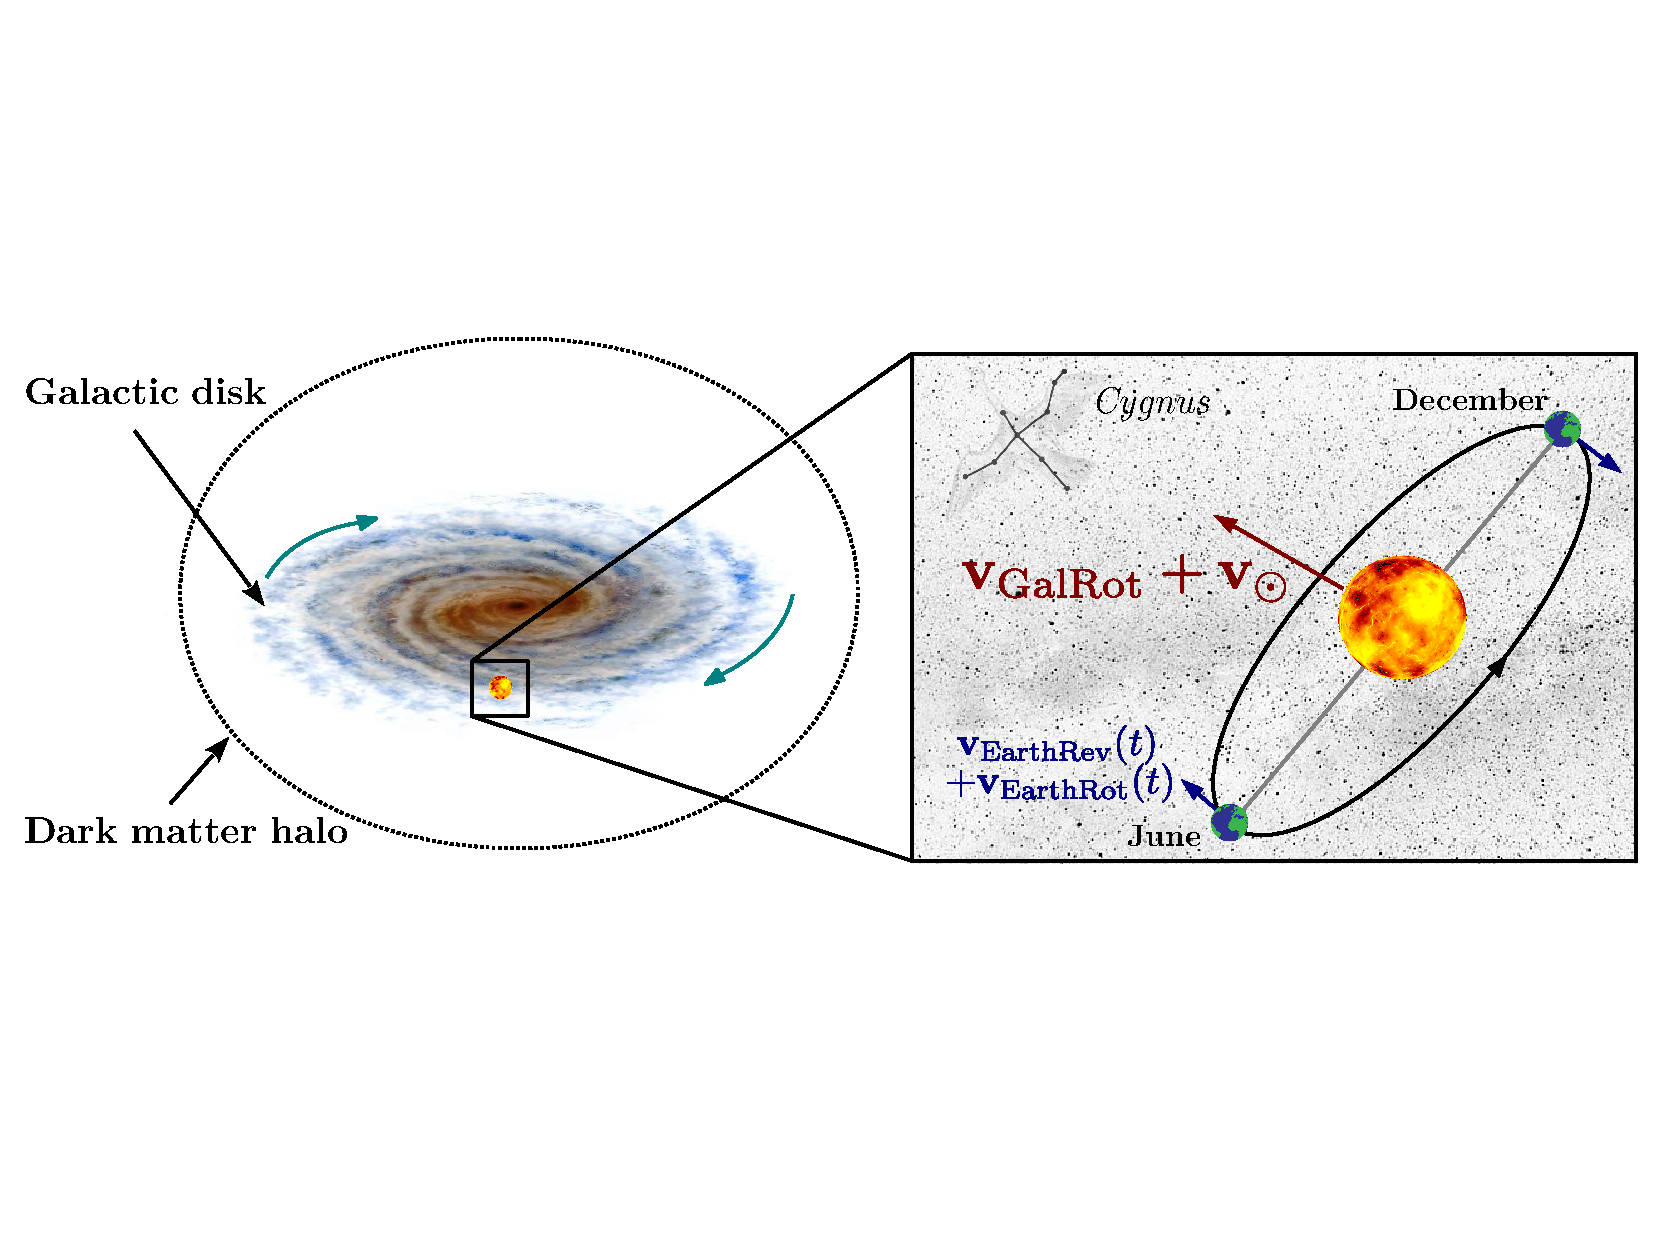
\includegraphics[trim = 0mm 50mm 0mm 50mm, clip, width=\textwidth]{Figures/labvelocity.pdf}
	\caption[Diagram of the components of the lab velocity]{Diagram of the components of the lab velocity.}
	\label{fig:labvelocity}
\end{figure}
The velocity distribution of WIMPs in the rest frame of the laboratory is obtained through a Galilean transformation of the Galactic frame distribution by the time dependent laboratory velocity ${\bf v}_{\rm lab}(t)$. This boost into the lab frame is responsible for time dependence, and for an isotropic Galactic frame distribution, is the sole source of the anisotropy in recoil directions (to be explored in Chapter~\ref{chapter:directional}). The lab velocity is,
\begin{equation}
\textbf{v}_\textrm{lab}(t) = {\bf v}_{\rm GalRot} + {\bf v}_\odot + {\bf v}_{\rm EarthRev}(t) + {\bf v}_{\rm EarthRot}(t) \, ,
\end{equation}
which is the sum of the bulk rotation of the local standard of rest (LSR) around the Galactic center, ${\bf v}_{\rm GalRot}$, the peculiar velocity of the Solar System with respect to the LSR, ${\bf v}_\odot$, the Earth's revolution around the sun, ${\bf v}_{\rm EarthRev}$, and the Earth's rotation, ${\bf v}_{\rm EarthRot}$.

When working in the laboratory frame we can use a North-West-Zenith coordinate system to describe each of these velocties. The astrophysical literature however will most often quote values in the Galactic coordinate system, ($U$,$V$,$W$), which point towards the Galactic center, the direction of Galactic rotation and the Galactic north pole respectively. We will also occasionally make use of Galactic longitude and latitude $(l,b)$ which are defined for a velocity $v$,
\begin{equation}
 \textbf{v} = v \, \begin{pmatrix} \cos l \cos b \\ \sin l \cos b \\ \sin b \end{pmatrix} \, .
\end{equation}

The dominant contribution to the lab velocity is ${\bf v}_{\rm GalRot}$. The velocity of the LSR is set up in Galactic coordinates as (0, $v_0$, 0) where $v_0$ is the circular rotation speed of the Milky Way. The value of $v_0$ is also the dominant source of uncertainty in $\textbf{v}_\textrm{lab}$. The standard value currently in use is $v_0\sim220$~km~s$^{-1}$~\cite{Kerr:1986hz}. The rotation of the Milky Way has been measured in various ways. For instance, measurements of the proper motions of nearby stars and Sgr A* located at the Galactic center can be used to constrain the quantity $(v_0+V_\odot)/R_\odot$ where $V_\odot$ is the second component of $\textbf{v}_\odot$ and $R_\odot$ is the Solar Galactic radius. Given independent constraints on the Solar peculiar velocity and radius one can combine measurements to arrive at a constraint on $v_0$. However, as noted by Lavalle \& Magni~\cite{Lavalle:2014rsa} because these estimates depend upon the prior assumptions made about other parameters, combining measurements of, for instance $R_\odot$ and $V_\odot$ from different sources may lead to spurious resulting values and underestimated errors. A study by McMillan \& Binney~\cite{McMillan:2009yr} for example found that values of the speed of the local standard of rest are heavily dependent on the model used for the rotation curve, quoting values of $v_0$ from $200 \pm 20$~km~s$^{-1}$ to $279 \pm 33$~km~s$^{-1}$. The peculiar velocity on the other hand is believed to possess a reasonably small uncertainty. A value commonly used from Schoenrich \etal~\cite{Schoenrich:2009bx} gives $\textbf{v}_\odot = (11.1,12.24,7.25)$~km~s$^{-1}$ in Galactic coordinates with roughly 1~km~s$^{-1}$ sized systematic errors. 

As shown in Fig.~\ref{fig:labvelocity} the velocities ${\bf v}_{\rm EarthRev}$ and ${\bf v}_{\rm EarthRot}$ are, respectively, responsible for the annual and diurnal~\cite{Bozorgnia:2011tk} modulation effects. For us they are known with effectively perfect precision. The calculation of these two components of the lab velocity and the necessary transformations between the Galactic and laboratory coordinate systems are presented in Appendix~\ref{app:labvelocity}. We display the time dependence induced in the total integrated event rate, $R$, due to these velocities in Fig.~\ref{fig:AnnualDailyModulation}. As can be seen, the phase and amplitude of the diurnal modulation is dependent on the location of the experiment.

\begin{figure}
\begin{center}
\includegraphics[width=0.95\textwidth]{Figures/AnnualDailyModulation.eps}
\caption[Annual and daily modulation signal]{Annual and daily modulation signal for three WIMP masses 50, 100 and 150 GeV (from top to bottom). The closeup shows the daily modulation signal for a 50 GeV WIMP for xenon target experiments located at three different locations. The event rate is calculated by integrating $\textrm{d}R(t)/\textrm{d}E_r$ over $E_r$ above a threshold which we set to 5 keV. The cross section in each case is $\sigma_p^{\rm SI} = 10^{-45}$~cm$^2$.}\label{fig:AnnualDailyModulation}
\end{center}
\end{figure}

\subsection{Velocity distribution}\label{sec:direct_fv}
The scattering rate is dependent on the Earth frame DM velocity distribution in the form of its mean inverse speed $g(\vmin,t)$. The true form of the local velocity distribution is unknown. However, unlike the lab velocity and local density, it cannot be measured astronomically. In principle only direct detection experiments have access to it. Hence we must pick a form for the distribution corresponding to a model for the Milky Way dark matter halo. If the density profile is analytic then the velocity distribution can be found by solving the Jeans equation. Alternatively a form can be extracted from the results of N-body or hydrodynamic simulations of Milky Way-like halos. As with the local density, the choice of $f(\textbf{v})$ will affect the predictions for the event rate. However the velocity distribution affects not just the total event rate but also the recoil energy dependence. This is an important but subtle point and can be exploited to give rise to considerable uncertainty in WIMP exclusion limits.

Most direct detection analyses are performed under a simple assumption for the Milky Way halo known as the standard halo model (SHM)~\cite{Green:2011bv}. This is a spherically symmetric isothermal halo model. Its $1/r^2$ density profile yields a Maxwell-Boltzmann (MB) velocity distribution with peak speed $v_0 = 220 \kms$ and dispersion\footnote{The relationship between the dispersion and circular speed is a consequence of a $1/r^2$ density profile, so relaxing this assumption means that $v_0$ and $\sigma_v$ are no longer connected.} $\sigma_v = v_0/\sqrt{2} \approx 156 \kms$. The distribution is most often truncated at the escape speed of the galaxy. The measurement from the radial velocity of RAVE stars is: $\vesc = 533^{+54}_{-41} \kms$~\cite{Piffl:2013mla}. The velocity distribution in the laboratory frame is therefore given by:
\begin{equation}\label{eq:shm}
f_\mathrm{SHM}(\mathbf{v},t) = \frac{1}{(2\pi \sigma_v^2)^{3/2}N_\mathrm{esc}} \, \exp \left( - \frac{|\mathbf{v} - \mathbf{v}_\textrm{lab}(t)|^2}{2\sigma_v^2}\right) \, \Theta (\vesc - |\mathbf{v} - \mathbf{v}_\textrm{lab}(t)|)\,, 
\end{equation}
with the normalisation constant,
\begin{equation}
N_\mathrm{esc} = \erf \left( \frac{\vesc}{\sqrt{2}\sigma_v}\right) - \sqrt{\frac{2}{\pi}} \frac{\vesc}{\sigma_v} \exp \left( -\frac{\vesc^2}{2\sigma_v^2}   \right)\,.
\end{equation}
Evaluating Eq.~(\ref{eq:gvmin}) for this velocity distribution gives for the mean inverse speed,
\begin{equation}\label{eq:gvmin_SHM}
g(\vmin,t) =
\begin{cases}
\frac{1}{v_\textrm{lab}(t)} & z<y\, , x<|y-z| \\
\frac{1}{2 N_{\rm esc} v_\textrm{lab}(t)} \left( \erf{(x+y)} - \erf{(x-y)} - \frac{4y}{\sqrt{\pi}} e^{-z^2}\right) & z>y \, , \, x<|y-z| \\
\frac{1}{2 N_{\rm esc} v_\textrm{lab}(t)} \left( \erf{(z)} - \erf{(x-y)} - \frac{2(y+z-x) }{\sqrt{\pi}} e^{-z^2}\right) & |y-z| < x<y+z \\
0 & y+z< x
\end{cases}
\end{equation}
where $x = \vmin/\sqrt{2}\sigma_v$, $y \equiv y(t) = v_{\rm lab}(t)/\sqrt{2}\sigma_v$ and $z = \vesc/\sqrt{2}\sigma_v$.

In order to maintain consistency when comparing experimental results it is important to establish some baseline halo model. The lack of a better motivated alternative and its simplicity mean the SHM can fill this role. Interestingly however, a number of recent hydrodynamic simulations suggest that a simple MB distribution may in fact be sufficient to describe the local velocity distribution \cite{Bozorgnia:2016ogo,Kelso:2016qqj,Sloane:2016kyi}. However many other hydrodynamic simulations, as well as earlier N-body simulations, presented persistent evidence for non-Maxwellian structure in Milky Way-like halos~\cite{Lisanti:2010qx,Kuhlen:2012ft,Fornasa:2013iaa,Butsky:2015pya}. The matter has not yet been conclusively settled and, critically for direct detection experiments, there is the possibility that the dark matter distribution at the Earth's Galactic radius could contain significant departures from the smooth isotropic properties of the SHM~\cite{Vogelsberger:2008qb,Maciejewski:2010gz,Mao:2012hf}. The velocity distribution may also contain additional features and substructures such as debris flows~\cite{Lisanti:2011as,Kuhlen:2012fz}, tidal streams~\cite{Freese:2003tt,Purcell:2012sh}, a co-rotating dark disk~\cite{Read:2009iv,Kuhlen:2013tra,Schaller:2016uot} or a `shadow bar'~\cite{Petersen:2016xtd,Petersen:2016vck}.

We consider two classes of substructure in this work which are motivated by results from N-body simulations, but also importantly have contrasting velocity structures so that they can be compared under a range of scenarios.

\textbf{Streams}: The local velocity distribution may contain substructure due to the tidal disruption and stripping of satellite galaxies or dark subhalos of the Milky Way. The slow accretion of material gives rise to a streams of dark matter particles wrapping the Galaxy some of which may intersect the stellar disk. Streams are seen generically in simulations of Milky Way-like galaxies as smaller subhalos become absorbed by their larger host and are in fact an inevitable consequence of the hierarchical growth of structure. There is also motivation for the existence of streams close to the Solar System. There have been observations in the past of collective linear motions of stars with narrow velocity dispersion consistent with a tail of stripped material from the nearby Sagittarius dwarf galaxy~\cite{Newberg:2003cu,Yanny:2003zu,Majewski:2003ux,Luque:2016nsz}. Furthermore simulations of the Sagittarius dwarf galaxy have found that the dark matter component of the stream could be significantly more extended than the stellar component and could hence give a sizable population of stream dark matter in direct detection experiments~\cite{Purcell:2012sh}.

If such a stream passed through the Solar System it would exist as a separate component of the local dark matter distribution with speeds tightly concentrated around a single velocity which would not necessarily be aligned with $\textbf{v}_\textrm{lab}$. We construct a model that assumes a fixed fraction of the local density is contained in the form of a tidal stream, described by Galactic frame velocity $\mathbf{v}_\textrm{str}$ and dispersion $\sigma_\mathrm{str}$. The velocity distribution of the stream is given by,
\begin{equation}
f_\mathrm{Str}(\mathbf{v},t) = \frac{1}{(2\pi \sigma_\textrm{str}^2)^{3/2}} \, \exp \left( - \frac{(\mathbf{v} - (\mathbf{v}_\textrm{lab}(t)+\mathbf{v}_\textrm{str}))^2}{2\sigma_\textrm{str}^2}\right) \,,
\end{equation}
and the full velocity distribution of the ``SHM+Str'' model is given by,
\begin{equation}
 f_\mathrm{SHM+Str}(\mathbf{v}) = \left(1-\frac{\rho_\mathrm{str}}{\rho_0}\right)f_\mathrm{SHM}(\mathbf{v},t) + \frac{\rho_\mathrm{str}}{\rho_0} f_\mathrm{Str}(\mathbf{v},t) \, .
\end{equation}
where $\rho_0$ is the SHM density and $\rho_\mathrm{str}$ is the stream density. The mean inverse speed for the stream has the same formula as for the SHM, Eq.~(\ref{eq:gvmin_SHM}) with $y~=~|\textbf{v}_\textrm{lab}(t)~+~\textbf{v}_\textrm{str}|/v_0$. Due to the spatially and kinematically localised nature of these features they give rise to prominent directional signatures in the recoil spectrum~\cite{Lee:2012pf,O'Hare:2014oxa}, as well as adding non-sinusoidal modifications to the annual modulation signals~\cite{Savage:2006qr}. 


\textbf{Debris flow}: Debris flows are another form of substructure that have appeared in N-body simulations such as Via Lactea II~\cite{Kuhlen:2008qj,Kuhlen:2012fz}. Like streams these are kinematically localised, characterised by a speed $v_f$, though unlike streams they are spatially extended features which form from the incomplete phase mixing of material during the formation of the halo. Following Ref.~\cite{Kuhlen:2012fz} we assume a model for the debris flow in which the velocity distribution is isotropic in the Galactic frame and a delta function in speed centered on $v_f$,
\begin{equation}
 f_\mathrm{DF}(\mathbf{v},t) = \frac{1}{4\pi v_f^2} \,\delta(|\mathbf{v}-\mathbf{v}_\textrm{lab}|-v_f) \, .
\end{equation}
So the distribution of a DF (in the laboratory frame) is a shell of radius $v_f$ centered on $\textbf{v}_\textrm{lab}$. Now, as with the SHM+Str model we combine the debris flow with the SHM as a fixed fraction of the local density:
\begin{equation}
 f_\mathrm{SHM+DF}(\mathbf{v},t) = \left(1-\frac{\rho_f}{\rho_0}\right)f_\mathrm{SHM}(\mathbf{v},t) + \frac{\rho_f}{\rho_0} f_\mathrm{DF}(\mathbf{v},t) \, .
\end{equation}
The mean inverse speed for this model is,
\begin{equation}
g(\vmin,t) =
\begin{cases}
\frac{1}{v_f} & \vmin < v_f-v_{\rm lab}(t) \\
\frac{v_f+v_{\rm lab}(t) - \vmin}{2v_f v_{\rm lab}(t)} & v_f-v_{\rm lab}(t)<\vmin <v_f+v_{\rm lab}(t) \\
0 & \vmin <v_f+v_{\rm lab}(t) \\
\end{cases}
\end{equation}

These benchmark velocity distributions along with the SHM are shown in Fig.~\ref{fig:polar}, while a summary of the benchmark parameter values used for each halo model is given in Table~\ref{tab:astrobenchmarks}. For the stream we use an estimate of the velocity of the Sagittarius stream from Ref.~\cite{Savage:2006qr}. However we assume that it comprises a significantly larger fraction of the local density than suggested by simulations, typically around the 1\% level~\cite{Vogelsberger:2008qb,Maciejewski:2010gz}. This allows us to make a clear distinction between our benchmark models. For the debris flow we use the parameters derived in the semi-analytic model of Ref.~\cite{Kuhlen:2012fz} based on the Via Lactea II simulation~\cite{Kuhlen:2008qj}. Although the debris flow in this simulation exhibited some velocity dispersion as well as a small bias towards directions tangential to the Galactic rotation, the simple isotropic model was found to capture the main features of the recoil spectrum.

Beside the benchmark velocity distributions in Fig.~\ref{fig:polar} we show sets of recoil energy spectra for a range of WIMP masses. For each benchmark model we see the same basic shape due to the SHM: an exponentially decreasing event rate which is cut off above some maximum energy set by the escape velocity. When streams and debris flows are included they induce an enhancement in the event rate for energies below a certain value which is set by the stream velocity or flow velocity respectively. 


\begin{table}[t]\centering
\ra{1.3}
\begin{tabularx}{\textwidth}{l|lll}
\hline\hline
\multirow{2}{*}{\bf Lab velocity}& Galactic rotation & $\textbf{v}_\textrm{GalRot}$ & (0, $v_0$, 0) km s$^{-1}$ \\
				 & Peculiar velocity & $\textbf{v}_\odot$ & (11.1, 12.24, 7.25) km s$^{-1}$ \\
\hline
\multirow{4}{*}{\bf SHM} & Local density & $\rho_0$ 		& $0.3 \, \mathrm{GeV} \, \mathrm{cm}^{-3}$\\
				& Circular speed & $v_0$ 	& $220 \kms$\\
				& Velocity dispersion& $\sigma_v$ 		& $156 \kms$\\
				& Escape speed& $\vesc$ & $533 \kms$\\
\hline
\multirow{3}{*}{{\bf Stream}}& Velocity & $\sigma_\textrm{str}$ 		& $10 \, \kms$\\
				& Dispersion& $\textbf{v}_\textrm{str}$ 	& $400\times(0,0.233,-0.970) \kms$\\
				& Density & $\rho_\textrm{str}/\rho_0$ 		& $0.1$\\
\hline
\multirow{2}{*}{{\bf Debris flow}} & Flow speed & $v_f$ 		& $340 \, \kms$\\
				& Density & $\rho_f/\rho_0$ 		& $0.22$\\
\hline\hline
\end{tabularx}
\caption[Astrophysical benchmark parameters]{Astrophysical benchmark parameters for the time independent components of the lab velocity, the standard halo model alone, stream and debris flow. In all examples, unless otherwise specified, the above parameters are used.}
\label{tab:astrobenchmarks}
\end{table}


\begin{figure}
\begin{center}
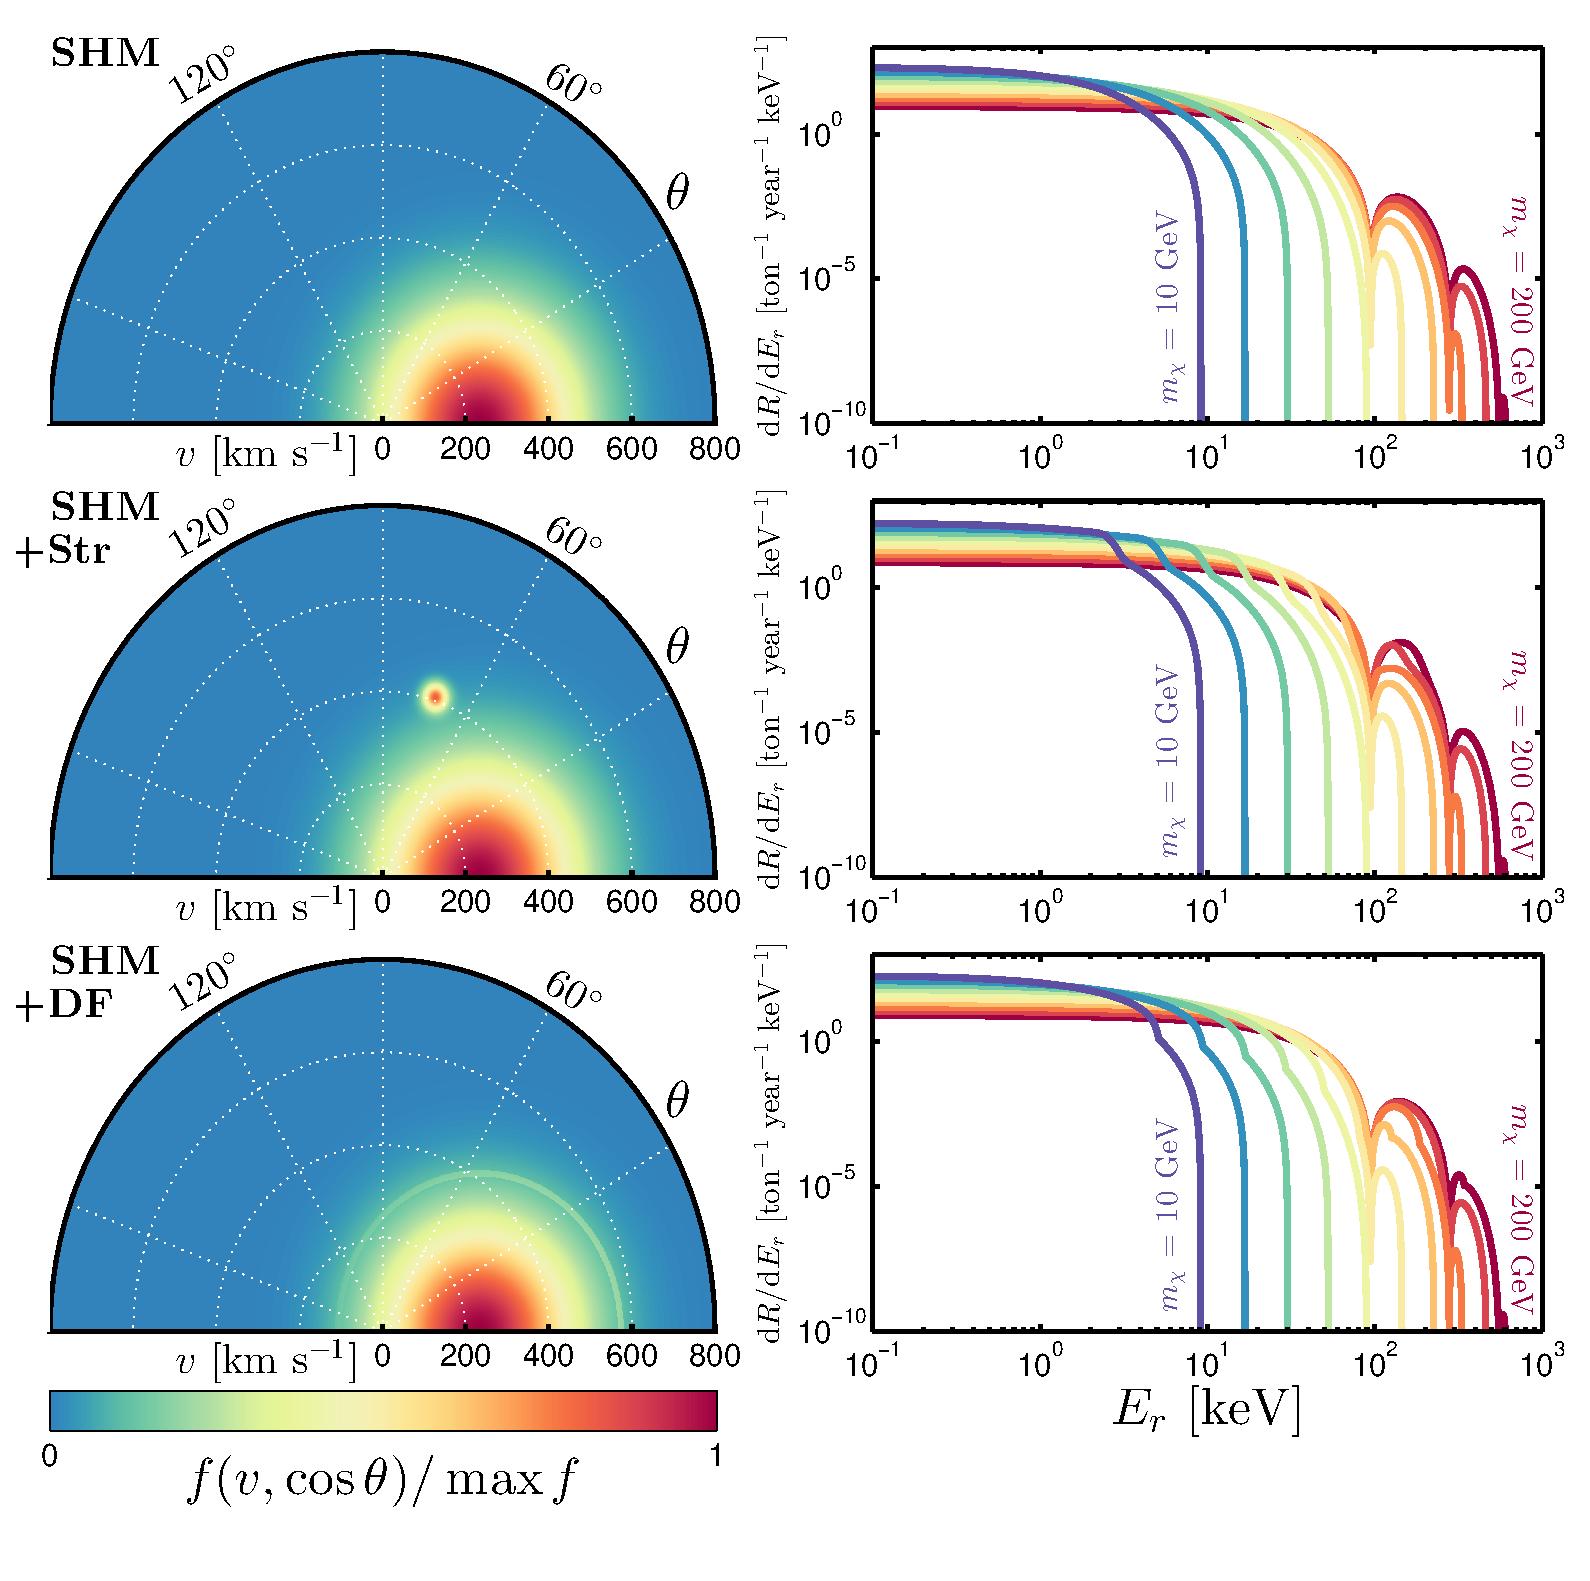
\includegraphics[width=0.97\textwidth]{Figures/fvEventRates.eps}\\
\caption[Benchmark velocity distributions and corresponding event rates]{ {\bf Left}: benchmark velocity distributions. We plot the velocity distribution for the SHM (top), SHM + Str (middle) and SHM + DF (bottom). The polar angle $\theta$ is measured with respect to $\mathbf{v}_\textrm{lab}$ and we have integrated $2\pi$ over the remaining azimuthal angle. {\bf Right:} corresponding SI xenon event rate energy spectra for each halo model over a range of logarithmically spaced masses between $m_\chi = 50$ to 200~GeV (blue to red).}\label{fig:polar}
\end{center}
\end{figure}
% shm should be 2pi larger than stream

Describing the velocity distribution is an important consideration for excluding or detecting dark matter in direct detection experiments. A failure to properly account for uncertainties in the DM velocity distribution may lead to biased measurements of the WIMP mass and cross section with a future signal~\cite{Peter:2011eu}. It will therefore be imperative to include these uncertainties in fits to direct detection data. This can be done by fitting to phenomenological models for the local distribution~\cite{Billard:2010jh,Lee:2012pf,O'Hare:2014oxa}, or by attempting to integrate out the astrophysics dependence of the DM signal so that comparisons can be made between exclusion limits from different experiments in a `halo-independent' way~\cite{Fox:2010bz,Fox:2010bu,Frandsen:2011gi,Gondolo:2012rs,DelNobile:2013cta,Fox:2014kua,Feldstein:2014gza,Anderson:2015xaa,Gelmini:2016pei,Kahlhoefer:2016eds,Ibarra:2017mzt}. Alternatively one can use empirical parameterisations of the speed distribution to account for astrophysical uncertainties, although this may lead to weakened constraints on other DM parameters~\cite{Peter:2011eu,Kavanagh:2013wba,Kavanagh:2013eya}. In the next Chapter we will explore model dependent and independent approaches for dealing with substructure in the velocity distribution with directional detectors.

\section{Experiments}\label{sec:direct_expts}
A direct detection experiment essentially consists of a fixed collection of particles called the `target' that are carefully monitored for the emission of certain signals (such as photons, charge or heat) which can be attributed to scattering events between the target and other particles. These particles can either be dark matter, or a background, which is anything else. In the event of an excess in the number of recoil events detected in the experiment over the expectation, then the measured $\textrm{d}R(t)/\textrm{d}E_r$ of those events can in principle be used to extract the properties of the WIMP. In the scenario that no unexplained excesses are detected then ranges of parameter values can be excluded. Real experiments are fraught with a range of complications related to backgrounds that we will now summarise. We also discuss some of the specific technological designs of certain current experiments and summarise the existing constraints.

\subsection{Backgrounds}
Dark matter scattering interactions are rare. Hence the most important factor for experiments to consider are backgrounds. To identify a signal which may produce less than $10^{-5}$ events per kg-day, ultra-low background conditions are needed. Backgrounds can be reduced at a number of stages. The first stage is to shield the detector volume as much as possible. Operating a detector deep underground or inside a mountain with a considerable distance of ground between the sky and the experiment can typically reduce the cosmic ray flux exponentially with (water equivalent) depth~\cite{Mei:2005gm}. Cosmic rays, in particular muons, must be shielded since they produce showers of up to GeV-scale neutrons in spallation reactions with the surroundings~\cite{Mei:2005gm}. Of all types of background particle, neutrons are the most problematic as their nuclear recoil signal, if they reach the detector, is almost identical to dark matter. 

In addition to cosmic backgrounds, both the environment and the experimental apparatus will be contaminated with radioactive isotopes. Radiogenically produced neutrons as well as Compton scattering and electron pair production due to $\gamma$ radiation are the most significant radioactive backgrounds. These require a second stage of background shielding surrounding the detector volume with additional layers of material such as lead or water tanks to veto environmental radiation. Water tanks can be used as `active' vetos which allow an experiment to reject events in the detector that are coincident with events in the water. Radioactive decays that are produced in the apparatus close to the detector, for example in the shielding itself, also need to be reduced as much as possible by carefully selecting especially radiopure materials. Decays produced due to impurities in the target material itself cannot be shielded so must be reduced as much as possible during manufacture. In detectors using crystalline materials such as CDMS, CRESST and CoGeNT, radioactive contaminants with large ionic radii such as radium, uranium and thorium are mostly rejected in the crystal growing process as they do not fit within the lattice spacing~\cite{Munster:2014mga}. Experiments using noble gases also have to contend with naturally occurring radioactive isotopes. Argon for example has a cosmogenically activated isotope ($^{39}$Ar) so experiments such as DarkSide find sources from deep underground~\cite{Back:2012pg}. In xenon the naturally occurring radioactive isotopes have half lives either short enough or long enough to not affect the experiment, but contamination from krypton and radon isotopes have led the XENON100, XMASS and LUX collaborations to develop special techniques to detect and extract quantities occurring at less than a part per quadrillion~\cite{Lindemann:2013kna}.

Whatever backgrounds that remain must be rejected at the level of the experimental design and analysis. The approach that has proven particularly powerful in certain experiments is electronic/nuclear recoil discrimination. WIMPs are much more likely to induce a nuclear recoil signal than an electron recoil signal meaning an experiment that can discriminate between the two can achieve a much greater level of sensitivity. Distinguishing between different sources of background is more efficient if an experiment can measure multiple types of signal from an event, e.g. scintillation photons, ionisation or phonons. WIMPs are also very unlikely to induce multiple scattering events compared with backgrounds. Linking series of recoil by either locating them in the detector volume or with time-tagging can be another useful approach for eliminating likely backgrounds. Additionally in experiments in which recoil sites are located, the outer layers of the detector volume itself can be used as a self-veto, with only the inner portion comprising the `fiducial' detector volume used for analysis. Ultimately though it is impossible to completely eliminate backgrounds so the final stages involve reducing backgrounds at the level of the analysis. This involves the modelling of backgrounds, use of detector calibration data, and defining signal regions in which the observed backgrounds are low. 

The final, though as yet unobserved, background to direct detection experiments are neutrinos from the Sun, the atmosphere as well as a cumulative emission from supernovae called the diffuse supernova background (DSNB). These cannot be shielded or rejected by any other means and dealing with them in standard direct detection experiments requires very high statistics~\cite{Billard:2013qya}. When direct detection experiments reach sizes large enough to observe a background due to coherent neutrino-nucleus scattering the large uncertainty on the expected neutrino flux compared with the low statistics expected from dark matter will limit discovery of certain masses where the two spectra overlap. We discuss the neutrino floor and approaches to deal with it in Chapter~\ref{chapter:nufloor}. 


\subsection{Current experiments}\label{sec:direct_current}
Direct detection experiments can be categorised based on the principle types of signal used to detect scattering events. All current experiments exploit at least one of three possible signals. These are: ionisation charge from liberated electrons/ions; scintillation photons from the excitation and de-excitation of electrons or nuclei in the target atoms; and phonons which are quantised vibrations such as heat or sound waves that propagate through solids. Many of the more recent experiments use a combination of two of these three detection channels. We now describe different broad categories of experimental design based on the state of the target material: noble gases, solid state and superheated fluids\footnote{We also discuss directional detectors in the next Chapter.}.

{\bf Noble gases}: Currently the most sensitive limits on SI cross sections for $m_\chi>20$ GeV are made by the dual phase xenon experiments, Xenon100~\cite{Aprile:2012nq}, LUX~\cite{Akerib:2016vxi}, and PandaX~\cite{Tan:2016zwf}. These experiments operate as time projection chambers (TPCs) in a design originally pioneered by ZEPLIN~\cite{Akimov:2006qw} and Xenon10~\cite{Aprile:2010bt} (the predecessor to Xenon100). The main detector volume is filled with liquid xenon with a smaller volume of gaseous xenon placed at the top of the main tank which collects ionised electrons drifted by an applied electric field. Photomultiplier tubes are arranged to detect both the photons produced as the drifted charge meets the gas phase xenon, as well as the prompt scintillation photons emitted from the initial scattering event. The yields from these different signals is dependent on the type of particle scattering so dual phase xenon TPCs can achieve excellent electronic/nuclear discrimination. Additionally the timing of the signals can be used to locate the event site inside the detector allowing a central fiducial volume to be selected for analysis that is self-shielded from backgrounds. The DarkSide~\cite{Agnes:2015ftt} experiment relies on the same technique but instead with an argon target. Alternatively noble gas experiments can operate solely in the liquid phase: with xenon again in the case of XMASS~\cite{Abe:2013tc} and argon for experiments such as DEAP~\cite{Boulay:2012hq} and MiniCLEAN~\cite{Rielage:2014pfm}. Single phase noble detectors only exploit the scintillation signal but resolve the timing of the received photons to give a `pulse shape' for each event. The advantage of argon in particular in this case is that the duration over which scintillation photons are produced for electronic and nuclear recoils are 6~ns and 1.6~$\mu$s~\cite{Boulay:2006mb} allowing excellent pulse shape discrimination.

{\bf Solid state}: There are two types of solid state detector: cryogenic experiments and crystal scintillators. Cryogenic bolometers such as SuperCDMS~\cite{Agnese:2014aze} and EDELWEISS~\cite{Hehn:2016nll} consist of a germanium target crystal cooled to mK temperatures combined with specialised detectors to measure liberated charge as well as phonons propagating through the solid after a scattering event. The advantage of these experiments are their extremely low energy thresholds. The dedicated single crystal experiment performed by SuperCDMS known as CDMSLite was selected to achieve a particularly low threshold of 0.8 keV (nuclear recoil energy) and currently sets the strongest limits around $m_\chi \sim 3$~GeV~\cite{Agnese:2015nto}. CoGeNT is also a cryogenic germanium experiment but measures only an ionisation signal and searches for an annual modulation to distinguish the signal from the background~\cite{Aalseth:2014eft}. CRESST on the other hand uses CaWO$_4$ crystals and exploits a combination of phonon and scintillation signals to achieve electronic/nuclear recoil discrimination with a 0.3 keV threshold; CRESST-II currently sets the strongest limits below 2 GeV~\cite{Angloher:2015ewa}. The other category of solid state detectors are crystal scintillators which are not operated cryogenically, instead designed to observe photons from molecules in the lattice excited by a scattering event. Scintillators such as DAMA/LIBRA~\cite{Bernabei:2008yh} and KIMS~\cite{Kim:2012rza} consist of collections of ultrapure crystals of NaI or CsI doped with thallium to improve the light emission and transparency of the material. Crystal scintillators have no signal discrimination capabilities so, like CoGeNT, search for an annual modulation in the event rate. DAMA report a 9.6$\sigma$ annual modulation signal with a phase consistent with a dark matter interpretation~\cite{Bernabei:2013xsa}. However the best fit cross sections and masses are ruled out by numerous other experiments\footnote{Arguments involving particle physics~\cite{DelNobile:2015lxa,Chang:2008gd}, astrophysical uncertainties~\cite{Belli:1999nz}, signal channelling~\cite{Savage:2008er} and many others have all been invoked to try and reconcile the tension between DAMA and other experiments.}. The issue has not yet been resolved. Results from experiments also using thallium doped NaI crystals: SABRE~\cite{Shields:2015wka}, Anais~\cite{Amare:2014jta} and DM-Ice~\cite{Cherwinka:2014xta}, will shed light on possible explanations for the signal.

{\bf Superheated fluids}: For spin-dependent (proton) interactions, experiments using superheated droplets of certain liquids: PICO~\cite{Amole:2015lsj,Amole:2015pla}, COUPP~\cite{Behnke:2012ys,Behnke:2008zza}, SIMPLE~\cite{Felizardo:2010mi} and PICASSO~\cite{Archambault:2012pm}, are currently most sensitive among direct detection searches. Superheated liquids are kept at temperatures just below their boiling point, if an event deposits enough energy inside a small enough volume then bubbles are nucleated and can be detected and located by a camera. The advantage of superheated fluids is that the ionising backgrounds from $\gamma$-rays and electrons cannot deposit a high enough energy density to be registered.  The liquids used in these experiments, CF$_3$I, C$_3$F$_8$ C$_2$ClF$_5$ and C$_4$F$_{10}$ all contain $^{19}$F which possesses a large $\langle S_p \rangle$. This has allowed superheated fluid experiments to set some of the strongest constraints on $\sigma_p^{\rm SD}$. 

% need to add new limit from PICO

\begin{figure}
\begin{center}
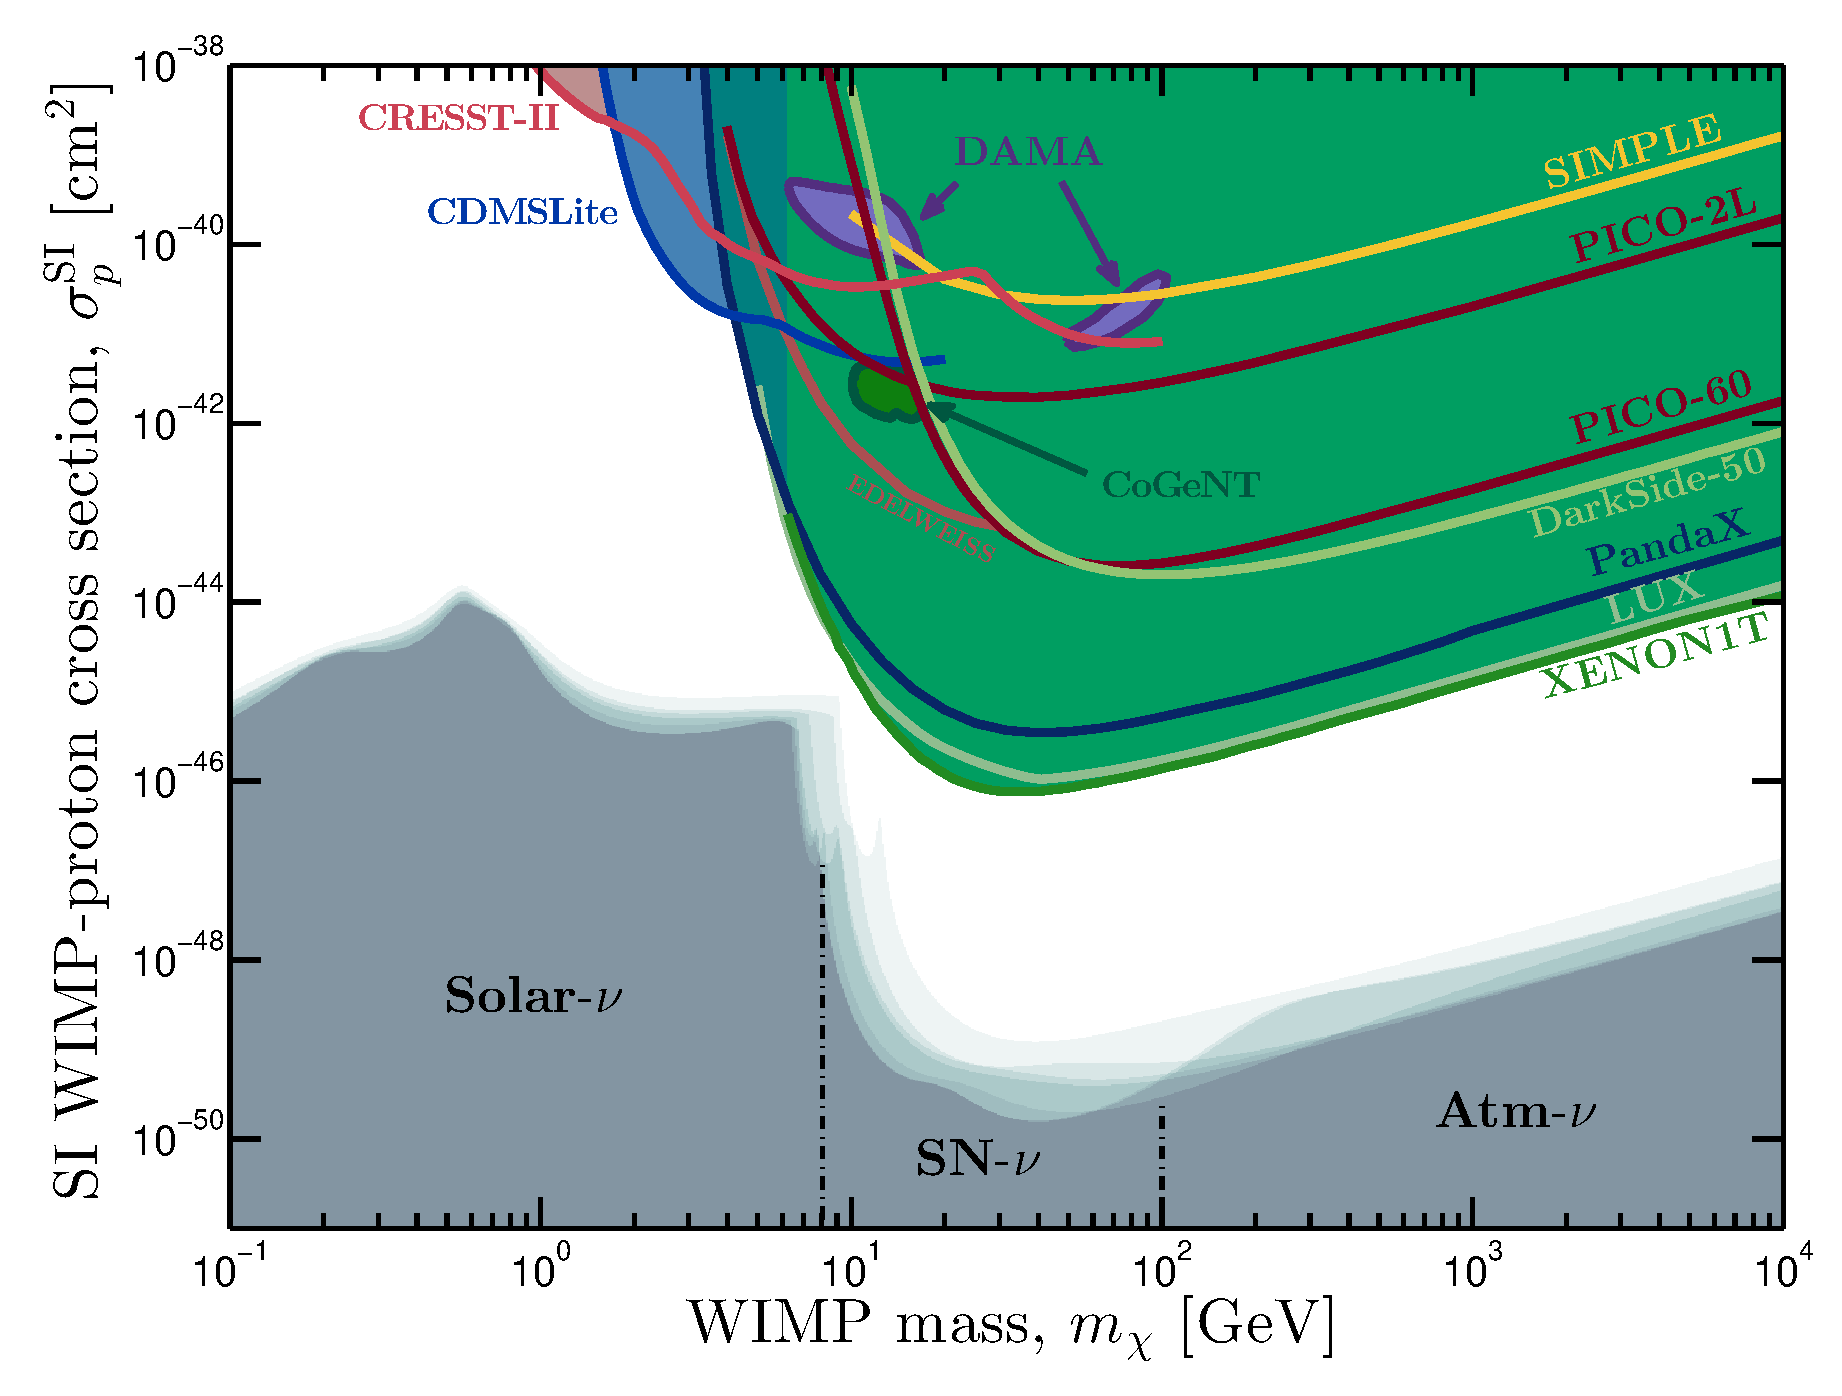
\includegraphics[width=0.9\textwidth]{Figures/WIMPlimits_SI.eps}\\
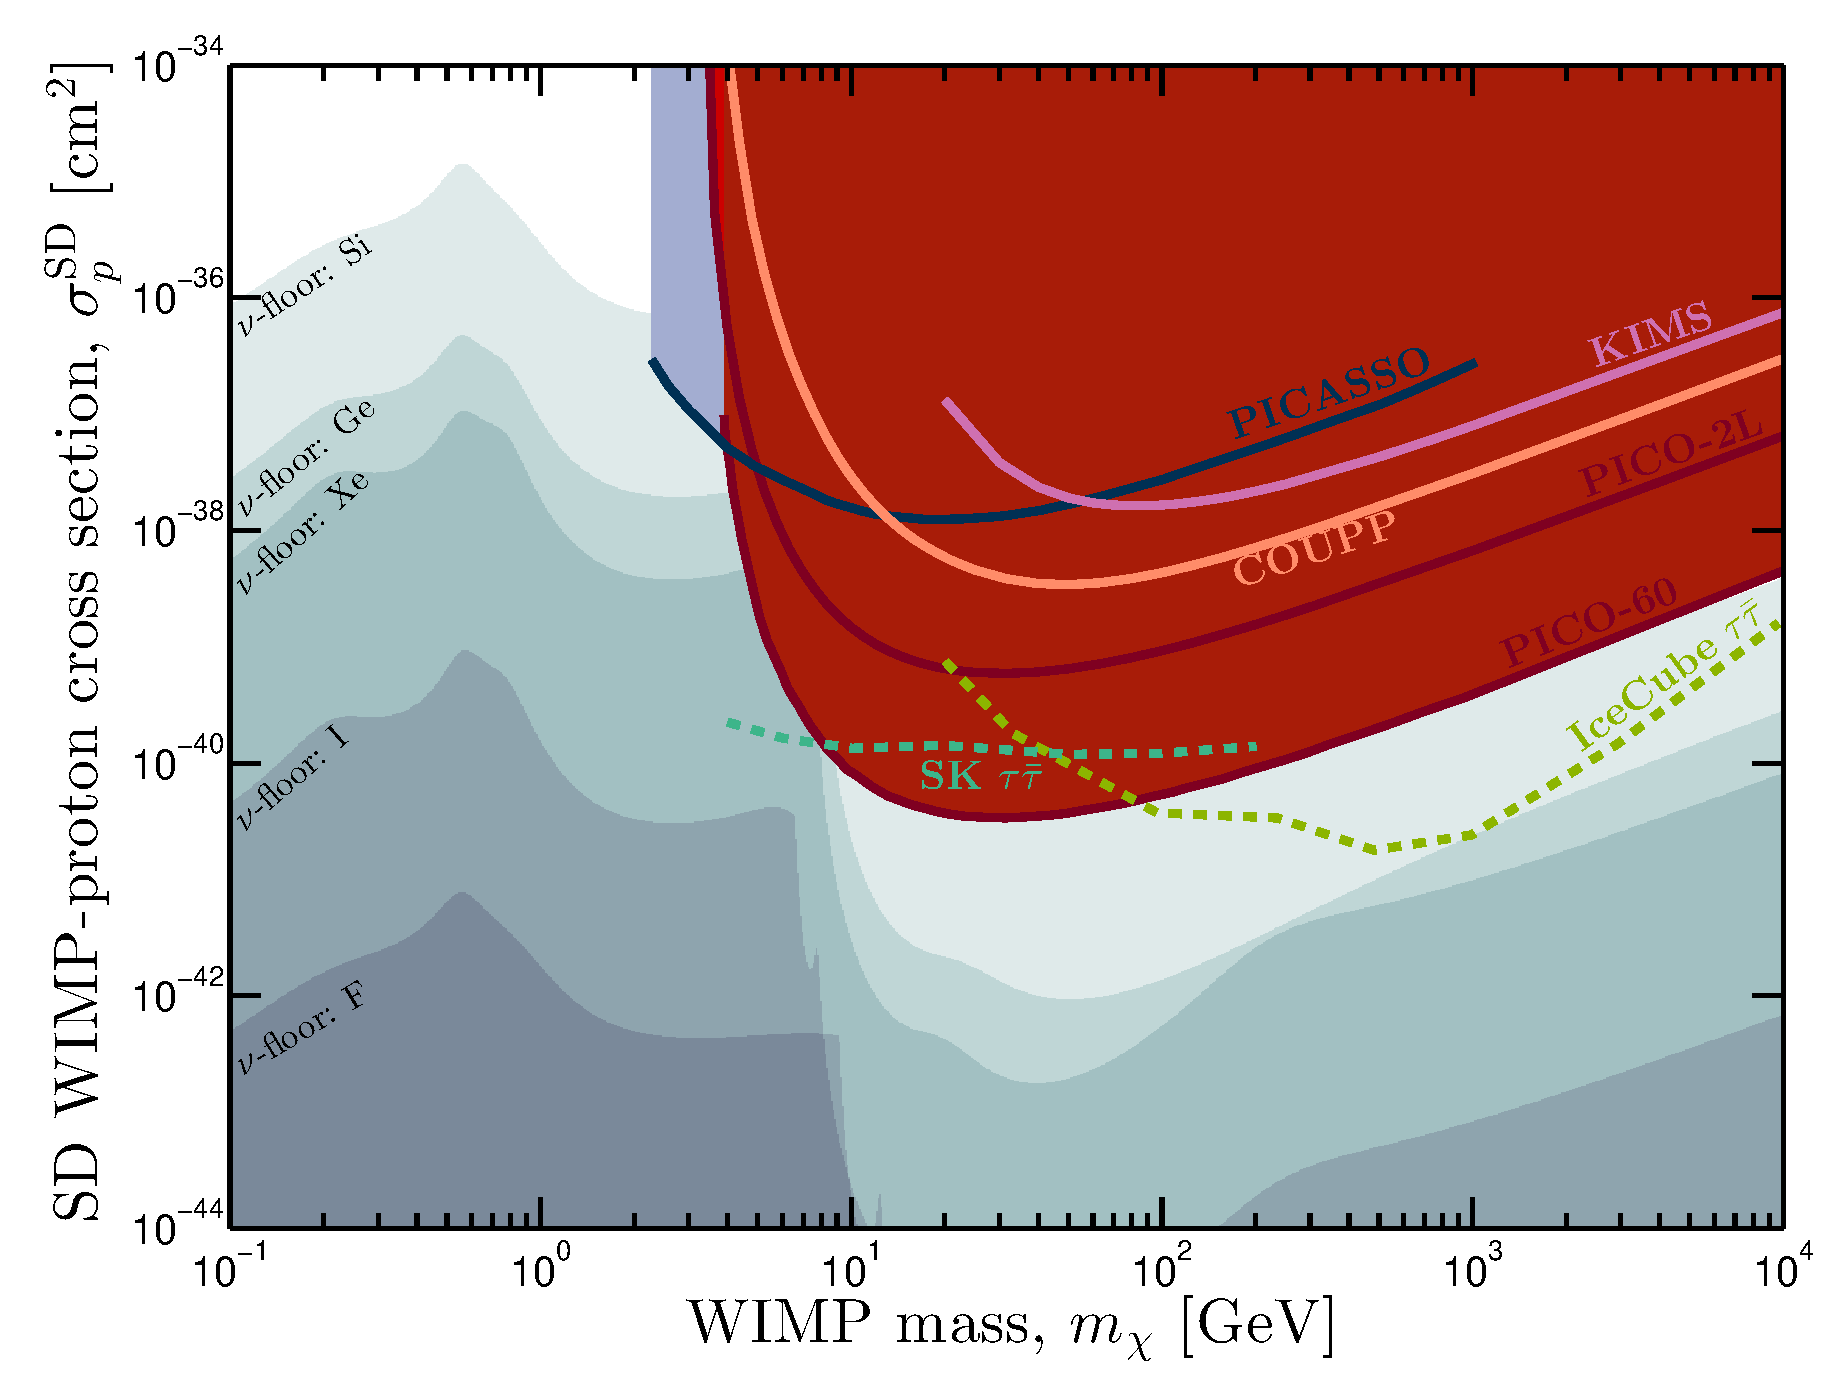
\includegraphics[width=0.9\textwidth]{Figures/WIMPlimits_SD.eps}
\caption[Current SI and SD WIMP exclusion limits]{Current excluded regions of the WIMP mass - proton cross section parameter space for spin-independent ({\bf top}) and spin-dependent ({\bf bottom}) interactions. The references for each limit are detailed in Table~\ref{tab:experiments}. The grey regions are neutrino floors for various target nuclei. In the top panel we indicate the dominant source of neutrino inducing the floor for different mass ranges: Solar neutrinos, the DSNB and atmospheric neutrinos.}\label{fig:WIMPlimits_SI}
\end{center}
\end{figure}


\begin{table}[t]\centering
\ra{1.3}
\begin{tabularx}{\textwidth}{c|YYYY}
\hline\hline
\quad		& {\bf Experiment}	& {\bf Target/Channel}	& {\bf Exposure \quad(kg days)} & {\bf Ref.} \\
\hline
\multirow{12}{*}{\bf SI:} 	& CDMSLite 		& Ge		& 70	& \cite{Agnese:2015nto}\\
				& CoGeNT	 	& Ge		& 1136	& \cite{Aalseth:2014jpa}\\
				& CRESST-II	 	& CaWO$_4$	& 52	& \cite{Angloher:2015ewa}\\
				& DAMA/LIBRA	 	& NaI		& 2.99$\times 10^6$& \cite{Savage:2008er}\\
				& DarkSide-50	 	& Ar		& 2617 & \cite{Agnes:2015ftt}\\
				& EDELWEISS	 	& Ge		& 496	& \cite{Hehn:2016nll}\\
				& LUX		 	& Xe		& 3.35$\times 10^4$& \cite{Akerib:2016vxi}\\
				& PandaX	 	& Xe		& 3.30$\times 10^4$	& \cite{Tan:2016zwf}\\
				& PICO-2L	 	& C$_3$F$_8$	& 211.5& \cite{Amole:2015lsj}\\
				& PICO-60	 	& CF$_3$I	& 3415& \cite{Amole:2015pla}\\
				& SIMPLE-II	 	& C$_2$ClF$_5$	& 30& \cite{Felizardo:2010mi}\\
				& Xenon100	 	& Xe		& 1.75$\times 10^4$& \cite{Aprile:2016swn}\\	
\hline
\multirow{5}{*}{\bf SD:} 	& COUPP		 	& CF$_3$I	& 437.4	& \cite{Behnke:2012ys}\\
				& KIMS			& CsI		& 2.45$\times 10^4$ & \cite{Kim:2012rza}\\
				& PICASSO	 	& C$_4$F$_{10}$	& 114& \cite{Archambault:2012pm}\\
				& PICO-2L	 	& C$_3$F$_8$	& 129& \cite{Amole:2016pye}\\
				& PICO-60	 	& C$_3$F$_8$	& 1167& \cite{Amole:2017dex}\\
\hline\hline
\multirow{2}{*}{$\boldsymbol{\nu}$:} 	& IceCube		 & $\chi\chi\rightarrow \tau\bar{\tau}$		& 532 days& \cite{Aartsen:2016zhm}\\
					& SK		 	& $\chi\chi\rightarrow \tau\bar{\tau}$			& 3903 days& \cite{Choi:2015ara}\\
\hline\hline
\end{tabularx}
\caption[Summary of WIMP direct detection experiments]{Summary of WIMP direct detection experiments and neutrino telescopes setting exclusion limits appearing in Fig.~\ref{fig:WIMPlimits_SI}.}
\label{tab:experiments}
\end{table}

We summarise the current status of direct detection experimental exclusion limits on both the SI and SD scattering cross sections in Fig.~\ref{fig:WIMPlimits_SI}. We list the targets, exposure and reference for each limit in Table~\ref{tab:experiments}. For the SD limits we also include the strongest indirect detection limits from neutrino telescopes IceCube and Super-Kamiokande. The limits displayed are excluded cross sections consisting of frequentist one-sided 90\% confidence intervals\footnote{Bayesian statistics are not widely used in experimental analyses but have been suggested as a means to compare multiple experiments, e.g. Ref.~\cite{Arina:2013jma}.}. There are several statistical procedures in use by different experimental collaborations to derive these exclusion limits. The choice of method depends on a number of factors relating to the knowledge of the background and the particular observables of the experiment. In cases when the underlying background can be modelled with simulations or measured with calibration data the profile likelihood ratio~\cite{Cowan:2010js} or Feldman-Cousins~\cite{Feldman:1997qc} methods are often used. For unknown or highly uncertain background conditions the maximum/optimum gap methods of Yellin~\cite{Yellin:2002xd} can be used instead which exclude cross sections based on events not appearing in certain signal intervals. In this thesis we derive limits based on mock experiments and use the profile likelihood ratio test detailed in Appendix~\ref{app:likelihood}.

The general shape of exclusion limits can be seen clearly in both panels of Fig.~\ref{fig:WIMPlimits_SI}: a sharp increase in cross section at the lowest mass extent of the limit moving towards a minimum at an intermediate mass between 10~-~100~GeV followed by a steady increase towards larger masses\footnote{Two limits in Fig.~\ref{fig:WIMPlimits_SI} deviate from this basic shape. CRESST-II has two kinks below 10 GeV which are due to the event rate transitioning between being dominated by the scattering of the three nuclei in CaWO$_4$; the kink above 10 GeV is due to the combination of the 2014 and 2015 analyses. In the CDMSLite the kink at 6 GeV is due to a particular emission line inside the detector.}. The sharp increase at low WIMP masses is due to the events from light WIMPs falling below the threshold of the experiment; lower thresholds implying smaller accessible $m_\chi$. The steady increase towards large masses is due to the decrease in the dark matter number density for heavier particles, assuming constant local density. Generally as the exposure of an experiment increases its limit will reach smaller cross sections over the full range of masses probed.

We will describe in detail the calculation of the neutrino floor in Chapter~\ref{chapter:nufloor} but we show the general appearance in the WIMP parameter space in Fig.~\ref{fig:WIMPlimits_SI}. An experiment with the naive sensitivity to reach WIMP cross sections below the grey regions will in fact have their discovery limited according to the floors shown. The shape of the floor is dependent on the energy spectrum of the WIMP signal so is dependent on target material. In the SI case this leads to only a shift by $A^2$ in cross section and a small shift in mass due to the recoil energy dependence on $m_N$. However in the SD case as well as the small shift in mass there are large differences in the cross section of the neutrino floor due to the dependence of $\mathcal{C}_{\rm SD}$ on the spin contents and isotopic fractions of the targets. For elements such as Si for example the isotopic fraction of the spin possessing isotope is very small, inducing a large upward shift in the regime of cross sections which produce similar event rates to the neutrino backgrounds. 

\subsection{Future experiments}\label{sec:direct_future}
Many of the experiments mentioned in the previous section are being upgraded or are merging with other collaborations. XMASS2~\cite{Hiraide:2015cba}, DEAP-3600~\cite{Boulay:2012hq}, Xenon1T/nT~\cite{Aprile:2015uzo}, DarkSide~\cite{Aalseth:2015mba} are planned or in construction upgrades to existing experiments. In addition, new collaborations have formed in recent years such as LZ~\cite{Akerib:2015cja}, EURECA~\cite{Angloher:2014bua} as well as DARWIN the proposed multi-ton xenon detector~\cite{Aalbers:2016jon}. This `next generation' of ton-scale detector are expected to be the first to detect coherent neutrino-nucleus scattering and reach the neutrino floor.

In addition to the tried and tested methods for rare event detection, the literature contains a wealth of alternative ideas which rely on upcoming or far-future technology. Some of these ideas are pointed particularly towards the light WIMP regime ($<$10~GeV) where much of the parameter space remains unexplored. New ideas such as the use of CCD chips in the DAMIC experiment~\cite{Barreto:2011zu} or experiments using $^4$He~\cite{Guo:2013dt} involve light targets so are ideal for low mass searches. However arguably the most powerful signal that one would hope to exploit in the future is directionality and there is considerable effort in constructing detectors that can measure recoil track directions. It may also be possible to adapt existing experimental technology in some directionally sensitive extension. We explore directional detection in detail in the next Chapter.

\section{Summary}\label{sec:direct_summary}
In this Chapter we have detailed the theoretical and experimental factors required for calculating signals in present and future direct detection experiments. We first discussed the ingredients from particle physics which predict spin-independent and spin-dependent event rates. We also outlined the astrophysical input from the local phase space distribution of dark matter in the Milky Way. We concluded with a discussion of the current status of the experimental direct detection effort with a summary of the various exclusion limits made on the WIMP cross section-mass parameter space. Now that we have established the status of direct detection the following Chapters will be forward-looking, exploring the future strategies we must employ to solve some of the problems we have already touched upon. We begin with directional detection experiments and how they may allow us to measure the dark matter distribution around us. We then look at how the neutrino floor will impact upcoming ton-scale experiments and describe how directional detectors will be required to overcome it.

\chapter{Directional detection}\label{chapter:directional}
\lhead{\emph{Directional detection}}

\section{Introduction}\label{sec:directional_intro}
It was first recognised by Spergel~\cite{Spergel:1987kx} that direct dark matter searches would be subject to a unique directional signature. The relative motion of the Solar System with respect to the largely non-rotating DM halo of the Milky Way should give rise to an anisotropic flux of WIMPs with a peak incoming direction pointing back to the constellation of Cygnus. This peak direction is typically regarded as a `smoking gun' signal for a particle of Galactic origin, as it cannot be mimicked by any known cosmic or terrestrial background. If a direct detection experiment were somehow able to measure an angular distribution of nuclear recoils consistent with the direction of Galactic rotation this would enable the conclusive discovery of dark matter~\cite{Copi:1999pw,Morgan:2004ys,Billard:2009mf,Green:2010zm,Mayet:2016zxu}. Crucially, the directional signature is also not shared by neutrinos, allowing the otherwise irreducible neutrino background to be distinguished from a WIMP signal~\cite{Grothaus:2014hja,O'Hare:2015mda}. The angular recoil spectrum also encodes much more information about the full three-dimensional velocity distribution than the recoil energy spectrum alone meaning a directionally sensitive experiment would be much better suited for probing the structure of the local DM halo~\cite{Billard:2010jh,Billard:2012qu,Lee:2012pf,O'Hare:2014oxa}. This in turn may give insights into the process of galaxy formation and the merger history of our own Milky Way. In this Chapter we focus on the latter of these three key motivations for the development of directional detection experiments. In the following Chapter, after we have introduced in detail the neutrino background we will explore how directional detectors can be used to circumvent the neutrino floor. 

We begin by introducing the necessary modifications one must make to the framework introduced in Chapter~\ref{chapter:direct} to account for the direction dependence of the WIMP-nucleus elastic scattering rate. We also summarise progress in the experimental implementation of directional detection, outlining some of the specific challenges present when measuring recoil directions that we must consider to evaluate realistic future prospects. We then detail two studies exploring how directional detectors can be used to probe the local dark matter velocity distribution and its substructure. First in Sec.~\ref{sec:directional_streams} we look at the particular case of tidal streams. We compare several statistical techniques for parametrically and non-parametrically detecting streams, beginning with a model for the Sagittarius stream and then moving to general streams. We then discuss model independent approaches for parameterising the full velocity distribution in Sec.~\ref{sec:directional_reconstruction}, comparing an empirical method with model dependent fits by testing them on the benchmark halo models introduced in Chapter~\ref{chapter:direct}. We conclude this chapter in Sec.~\ref{sec:directional_finalremarks} with some final remarks.

\section{Directional detection formalism}
\subsection{Rate calculation}\label{sec:directional_rates}
We can insert a dependence on recoil direction $\hat{\textbf{q}}$ into the formula we have already introduced for the event rate $\textrm{d}R/\textrm{d}E_r$ by enforcing the kinematical relationship between the recoil energy and direction,
\begin{equation}
 \cos{\theta} = \sqrt{\frac{m_N E_r}{2 v^2 \mu^2_{\chi N}}} = \frac{\vmin}{v} \, .
\end{equation}
We can insert this angular dependence into the cross section by introducing a solid angle element around the recoil direction $\textrm{d}\Omega_r = 2\pi \textrm{d} \cos{\theta}$ where we have exploited the azimuthal symmetry around the recoil direction to give the factor of $2\pi$. We enforce the above constraint on the recoil angle $\theta$ with a $\delta$-function,
\begin{equation}
 \frac{\textrm{d}^2\sigma}{\textrm{d}E_r\textrm{d}\Omega_r} = \frac{\textrm{d}\sigma}{\textrm{d}E_r} \frac{1}{2\pi}\ \delta \left( \cos{\theta} - \frac{\vmin}{v}\right) \, .
\end{equation}
We can introduce the recoil direction vector $\hat{\textbf{q}}$ by rewriting the angle $\theta$ as, $\cos{\theta}~=~\textbf{v}~\cdot~\hat{\textbf{q}}/v$ so we have for the double differential cross section,
\begin{equation}
 \frac{\textrm{d}^2\sigma}{\textrm{d}E_r\textrm{d}\Omega_r} = \frac{\textrm{d}\sigma}{\textrm{d}E_r} \frac{1}{2\pi} v \, \delta \left(\textbf{v} \cdot \hat{\textbf{q}} - \vmin\right) \, .
\end{equation}
This now modifies the formula for the event rate. In the non-directional case $\textrm{d}R/\textrm{d}E_r$ depends upon the velocity distribution in terms of the mean inverse speed $g(\vmin,t)$. In the directional case the analogous $\textrm{d}^2 R/\textrm{d}E_r\textrm{d}\Omega_r$ includes a $\delta$-function enforcing the kinematics. This requires the `Radon transform' of the velocity distribution~\cite{Radon,Gondolo:2002np}, which is an integral transform most commonly used in medical CT scans. It is defined,
\begin{equation}
 \hat{f}(\vmin,\hat{\textbf{q}},t) = \int \delta\left(\textbf{v} \cdot \hat{\textbf{q}} - \vmin\right) f(\textbf{v}+\textbf{v}_\textrm{lab}(t))\, \textrm{d}^3 \textbf{v}\, .
\end{equation}
We show the geometric interpretation of the Radon transform in Fig.~\ref{fig:radontransform}. The Radon transform integrates over velocities that lie along a plane perpendicular to the recoil direction that is a distance $\vmin$ away from the origin.
\begin{figure}
	\centering
	%trim option's parameter order: left bottom right top
	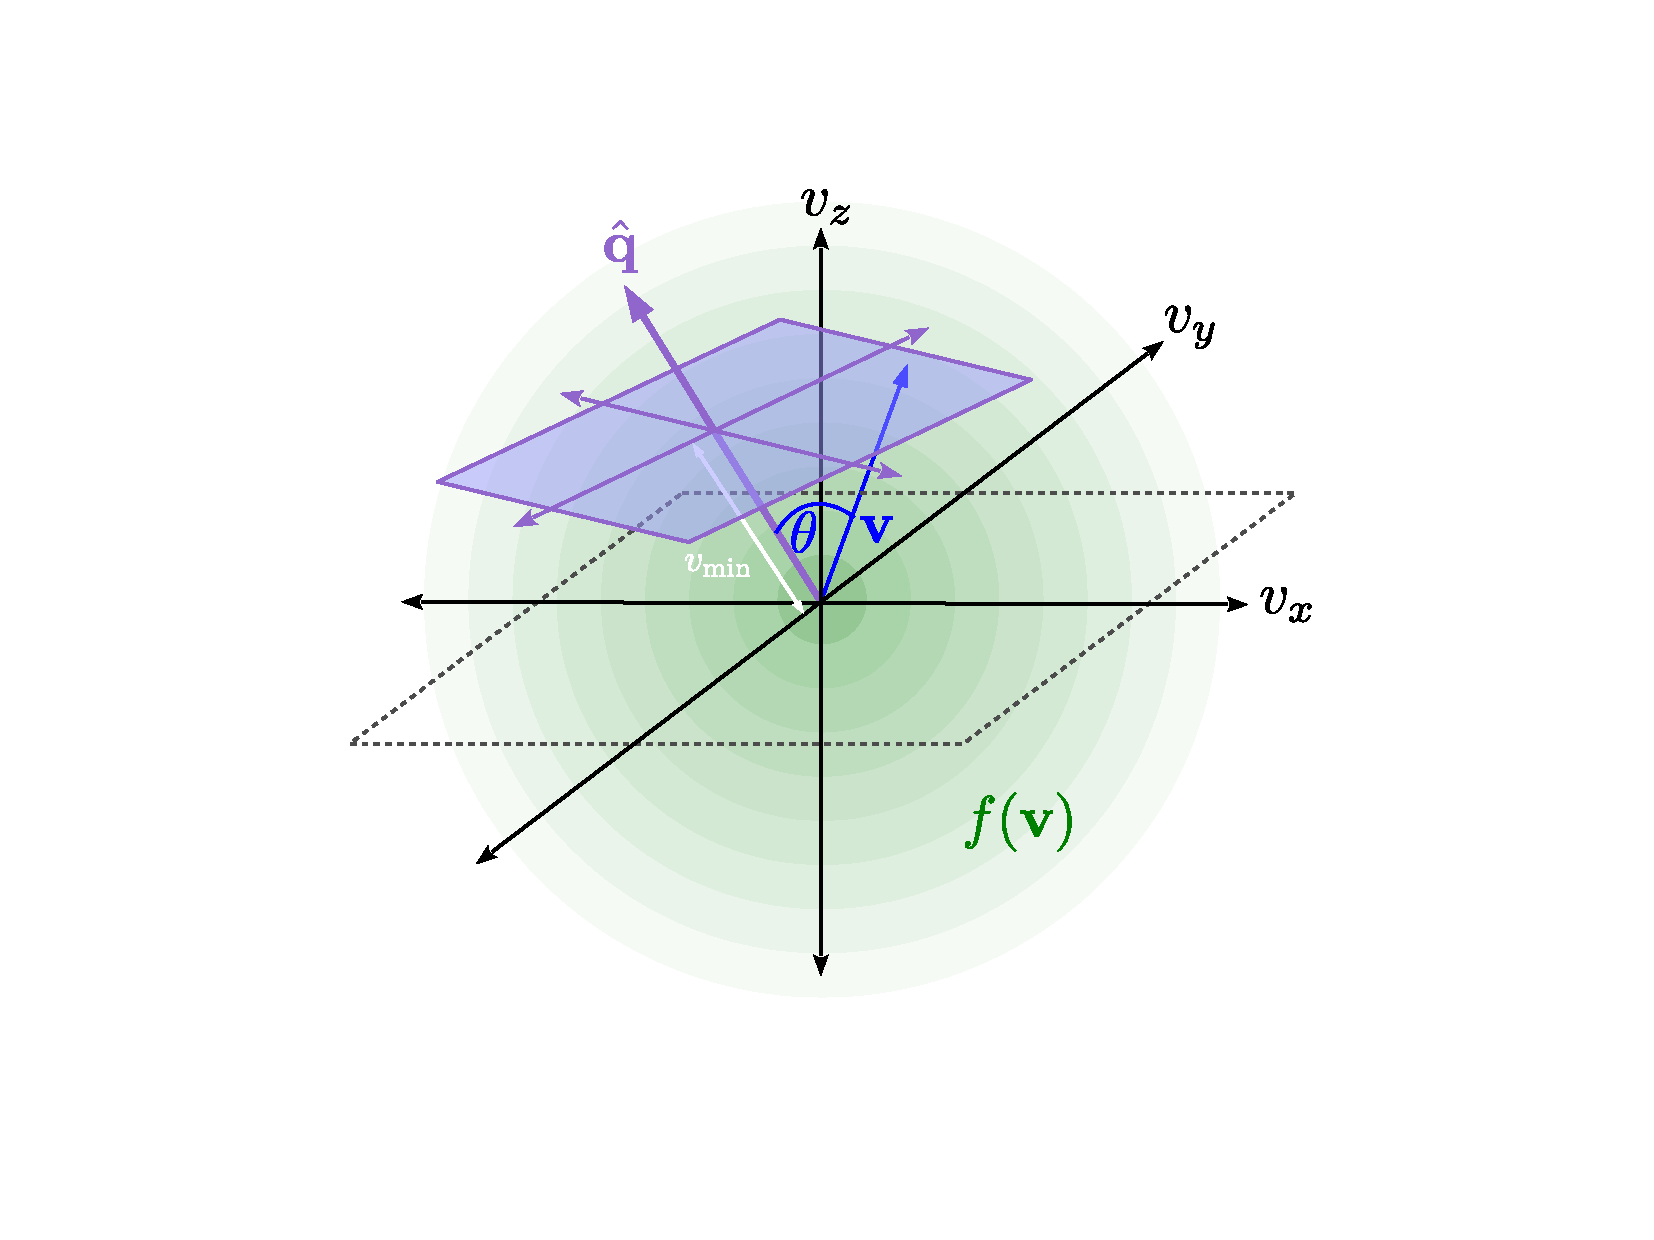
\includegraphics[trim = 20mm 30mm 20mm 20mm, clip, width=\textwidth]{Figures/radontransform.pdf}
	\caption[Diagram showing the geometry of the Radon transform]{Diagram showing the geometric interpretation of the Radon transform. The velocities $\color{blue}{\textbf{v}}$ of the distribution $\color[rgb]{0,0.5,0}{f(\textbf{v})}$ that contribute to the event rate for a particular $v_\textrm{min}$ and recoil direction $\color[rgb]{0.5686    0.4000    0.8000}{\hat{\textbf{q}}}$ are those which lie along the plane shown in purple. The plane is perpendicular to $\color[rgb]{0.5686    0.4000    0.8000}{\hat{\textbf{q}}}$ and is a distance $\vmin$ away from the origin. Thus the radon transform $\hat{f}(\vmin,\hat{\textbf{q}})$ is the integral of $\color{blue}{\textbf{v}}$ over the plane.}
	\label{fig:radontransform}
\end{figure}

In analogy with Eq.~(\ref{eq:finaleventrate}) we can write the general formula for the directional event rate,
\begin{equation}\label{eq:finaleventrate-directional}
 \frac{\textrm{d}^2R(t)}{\textrm{d}E_r\textrm{d}\Omega_r} = \sum_{i=1}^n \zeta^i \frac{\rho_0}{4\pi\mu_{\chi p}^2 m_\chi} (\sigma^{\rm SI}_p \mathcal{C}^i_{\textrm{SI}} F^2_{\rm SI}(E_r) + \sigma^{\rm SD}_p \mathcal{C}^i_{\textrm{SD}} F^2_{\rm SD}(E_r))  \, \hat{f}(\vmin,\hat{\textbf{q}},t) \, .
\end{equation}
This formula is very similar to the non-directional rate except we have picked up a factor of $1/2\pi$ and require $\hat{f}(\vmin,\hat{\textbf{q}},t)$ instead of $g(\vmin,t)$.

For the Maxwell-Boltzmann distribution of the SHM the Radon transform is,
\begin{equation}
\hat{f}_{\rm SHM}(v_{\text{min}},\hat{\bf{q}}, t) =
\begin{cases}
\frac{\exp{\left(-\frac{\left|v_{\text{min}} + \hat{\bf{q}}\cdot{\bf v}_{\rm lab}(t)\right|^2}{2\sigma^2_v}\right)} - \exp{\left(-\frac{v_{\rm esc}^2}{2\sigma^2_v}\right)}}{N_{\rm esc}(2\pi\sigma_v^{2})^{1/2}} & (\vmin + \hat{\textbf{q}} \cdot  \textbf{v}_\textrm{lab}(t))< \vesc \\
0 & (\vmin + \hat{\textbf{q}} \cdot  \textbf{v}_\textrm{lab}(t))> \vesc \, .
\end{cases}
\end{equation} 
While for the stream we have the same functional form but we replace $\sigma_v$ with $\sigma_{\rm str}$ and $\textbf{v}_\textrm{lab}$ with $\textbf{v}_\textrm{lab}+\textbf{v}_\textrm{str}$. 

For the debris flow we have the following form for the Radon transform,
\begin{equation}
\hat{f}_{\rm DF}(v_{\text{min}},\hat{\bf{q}}, t)  = 
\begin{cases}
0 & (\vmin + \hat{\textbf{q}} \cdot  \textbf{v}_\textrm{lab}(t))> v_f \\
\frac{1}{2v_f} & (\vmin + \hat{\textbf{q}} \cdot  \textbf{v}_\textrm{lab}(t))< v_f 
\end{cases}
\end{equation}
Because the distribution of a debris flow is a shell of radius $v_f$ centered on $\textbf{v}_\textrm{lab}$, its Radon transform is the integral along the circle that is the intersection of this shell and the plane shown in Fig.~\ref{fig:radontransform}.


\subsection{Resulting signals}\label{sec:directional_signals}
\begin{figure}
	\centering
	%trim option's parameter order: left bottom right top
	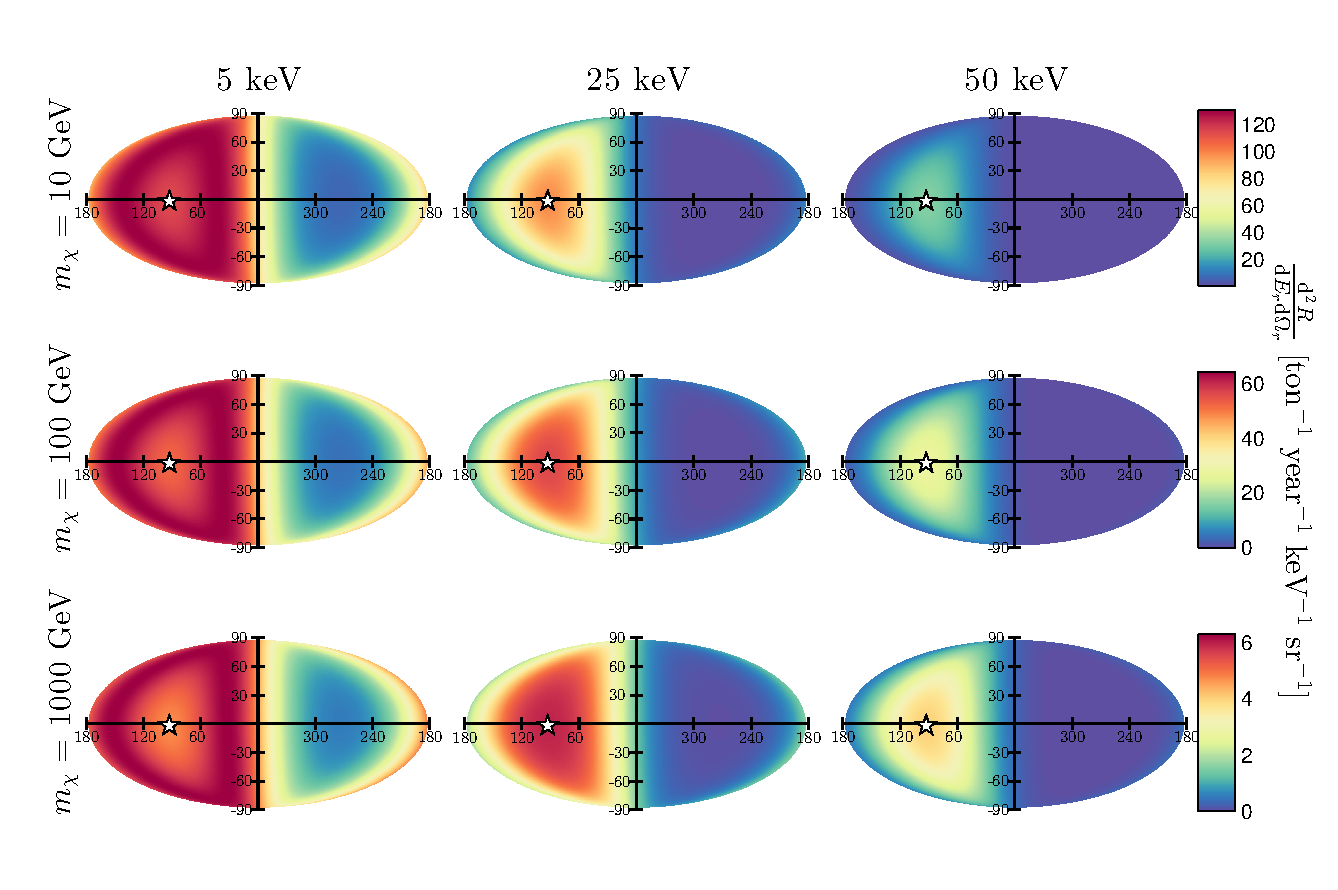
\includegraphics[trim = 0mm 0mm 0mm 0mm, clip, width=\textwidth]{Figures/skymaps_mchi.eps}
	\caption[Directional recoil skymaps for three WIMP masses]{Mollweide projections of the full sky recoil maps for three recoil energies: 5 keV, 25 keV and 50 keV corresponding to the three columns. The rows indicate recoil spectra for three WIMP masses $m_\chi = $ 10, 100 and 1000~GeV scattering with a $^{19}$F target. The axes represent Galactic coordinates $(l,b)$ where the direction of $\textbf{v}_\textrm{lab}$ is marked with a star.}
	\label{fig:skymaps_mchi}
\end{figure}

The event rate of Eq.~(\ref{eq:finaleventrate-directional}) gives rise to a range of unique directional signatures. The primary signal is a dipole anisotropy towards the direction $\hat{\bf{q}} = -{\bf v}_{\rm lab}$ as can be seen in Fig.~\ref{fig:skymaps_mchi} where we show the event rate as a function of energy and direction which clearly peaks along the plane of the Galaxy. As first calculated in Ref.~\cite{Spergel:1987kx} this would result in an $\mathcal{O}(10)$ forward-backward asymmetry in the number of recoils. In Fig.~\ref{fig:skymaps_mchi} and subsequent skymaps we use a Mollweide projection to map the 3-dimensional recoil spectrum onto the 2-d plane. We follow the convention used in directional detection literature to display recoil maps as the directions from which the recoils originate (as one would in astronomy) rather than the direction the recoils vectors point. In other words, the axes of the projection correspond to $-\hat{\textbf{q}}$ rather than $\hat{\textbf{q}}$. This is why the skymaps peak around the point marked by $\textbf{v}_\textrm{lab}$. This direction lies along the Galactic plane ($b_{\rm lab}~\approx~0$) and towards the direction of Galactic rotation ($l_{\rm lab}~\approx~90^\circ$), but is slightly offset by the Solar peculiar velocity $\textbf{v}_\odot$.

Because we assume an isotropic assumption for the Galactic frame velocity distribution the recoil maps are symmetric about the direction $\textbf{v}_\textrm{lab}$. The recoil directions also become less angularly dispersed towards higher recoil energies which preserve more of the original incoming WIMP direction. The prominence of the dipole feature means that in ideal circumstances (i.e. perfect recoil direction reconstruction) an isotropic assumption for the recoil direction distribution can be rejected at 90\% confidence with only $\mathcal{O}(10)$ events, with no recoil energy information needed~\cite{Green:2010zm}. With $\mathcal{O}(30)$ recoil directions it becomes possible to point back towards Cygnus and confirm the Galactic origin of the signal~\cite{Billard:2009mf}.

It was noted in Ref.~\cite{Bozorgnia:2011vc} that for recoil energies where $v_{\rm min}<v_{\rm lab}$ the directional rate is maximised for directions that satisfy $\hat{\bf{q}}\cdot{\bf v}_{\rm lab} = -v_{\rm min}$. At these energies the recoil pattern forms a ring around $\textbf{v}_{\rm lab}$, rather than a dipole. This occurs only for low energies and large WIMP masses but can be used as a secondary signal in directional detection as its radius would provide a measure of $m_\chi$. The ring feature has an angular radius of $\cos^{-1}(\vmin/v_\textrm{lab})$ and can be seen in Fig.~\ref{fig:skymaps_mchi} in the maps at $E_r = 5$~keV, most prominently in the $m_\chi=1000$~GeV case. Additionally, once the correlation with the time dependence is included then an aberration of the recoil pattern is observed (in analogy with the aberration of the position of stars in the sky due to the Earth's orbit~\cite{Bozorgnia:2012eg}). In our analyses we do not consider the ring or aberration features separately, as in Refs.~\cite{Bozorgnia:2011vc, Bozorgnia:2012eg} for example, but because they are embedded in the analytic description of the event rate they are included in likelihood fits automatically.

\subsection{Experiments}\label{sec:directional_expts}
The strength of directional detection as a tool for dark matter discovery relies on the fact that no known backgrounds are believed to mimic (or even have any relation to) the directionality of the dark matter signal. In fact most backgrounds should be close to isotropic. Certainly in the case of radiogenic neutrons an essentially isotropic background is expected. Cosmic muon induced neutrons would not necessarily be expected to be perfectly isotropic, however past studies~\cite{Mei:2005gm} have found only a very small downward-going excess due to the directionality of spallation reactions. The elastic scattering process also washes out much of the directional preference in the flux of incoming particles so any backgrounds would need to be very strongly anisotropic to affect the discovery reach of a directional experiment.

\begin{figure}
	%trim option's parameter order: left bottom right top
	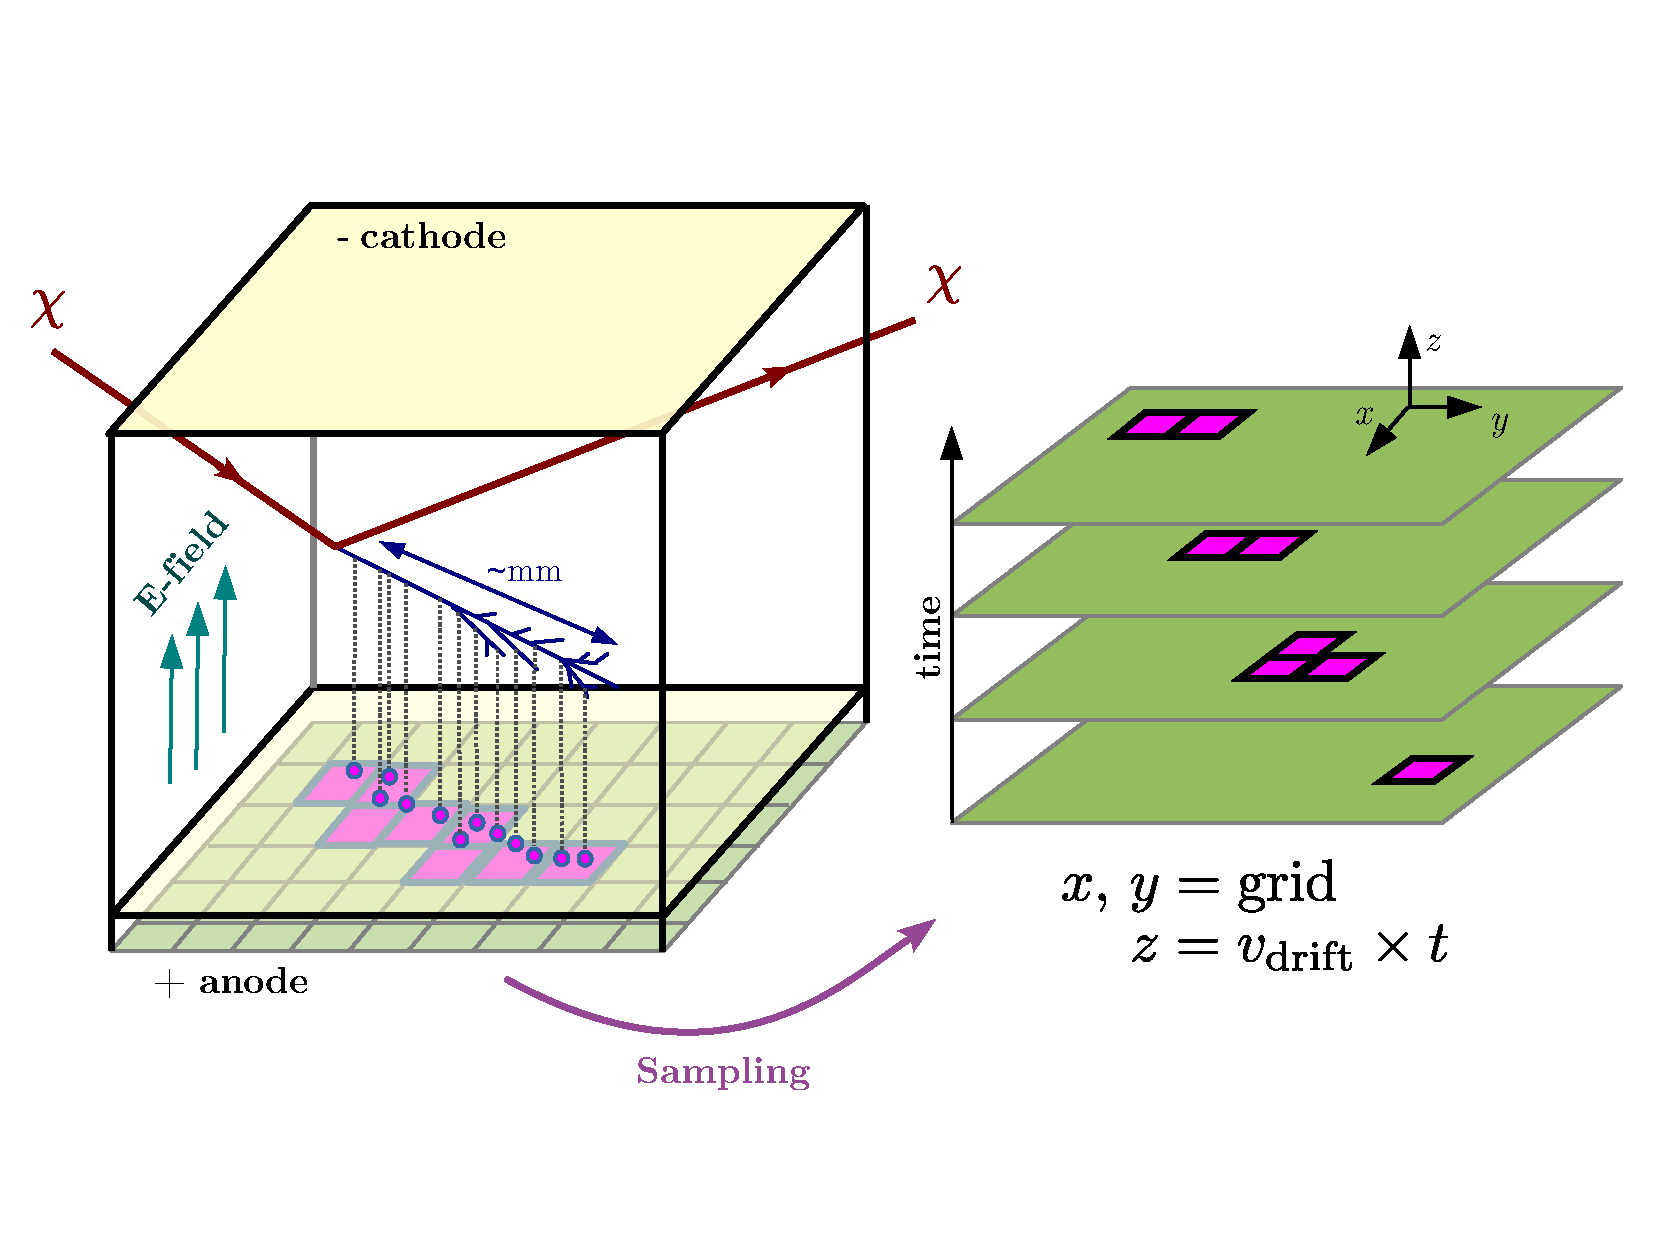
\includegraphics[trim = 0mm 20mm 0mm 20mm, clip, width=\textwidth]{Figures/TPC.pdf}
	\caption[Diagram of a low pressure gas TPC]{Diagram of a low pressure gas TPC with a pixel chip readout.}
	\label{fig:TPC}
\end{figure}

Measuring the direction of nuclear recoils at the keV scale is experimentally challenging. A variety of prototype experiments are currently in operation utilising a range of novel techniques to extract directional information from a nuclear recoil signal (see e.g.~Refs.~\cite{Cappella:2013,Capparelli:2014lua,Aleksandrov:2016fyr}, as well as Ref.~\cite{Ahlen:2009ev} for a review). One promising approach is to use a gaseous TPC at low pressure ($\sim$ 0.1 atm) in order for the track of electrons ionised by a nuclear recoil to be large enough to detect at around $\mathcal{O}(1\,{\rm mm})$ in size. In Fig.~\ref{fig:TPC} we show a diagram of how a low pressure TPC measures the components of a recoil track in three dimensions. The direction of this recoil can be inferred by drifting the ionisation-induced electron cloud to a time sampled pixelised anode usually based on CCD technology. The location on the grid of the measured charge provides a two dimensional projection of the track whereas the time sampling of the anode can be converted into the projection onto the drift direction assuming knowledge of the drift speed of the electrons through the gas, $v_{\rm drift}$. In principle these two effects can be combined to reconstruct the 3-dimensional orientation of the track. Experiments such as MIMAC~\cite{Riffard:2013psa,Riffard:2016mgw}, DRIFT~\cite{Daw:2011wq,Battat:2014van}, NEWAGE~\cite{Nakamura:2015iza,Miuchi:2010hn}, DMTPC~\cite{Monroe:2011er,Leyton:2016nit} and D3~\cite{Jaegle:2011rn} currently make use of this technology in some variant. 

Attempts to measure recoil directionality encounter a range of experimental difficulties on top of the usual challenges of direct detection. The most obvious limitation of low pressure TPCs operating in the gas phase is their ability to be scaled to competitive detector masses which would require prohibitively large volumes. The largest of these prototype experiments currently has only a 0.1 kg active volume~\cite{Santos:2011kf}, though a much larger WIMP `observatory' is a possibility~\cite{Simpson:2017aaa}. In terms of the operation of a directional TPC however, the greatest challenges are those that arise in attempting to accurately reconstruct the recoil track. Primarily this is because the detected track is not a perfect representation of the initial recoil direction $\hat{\textbf{q}}$. In practice experiments suffer from an effect known as `straggling' as the recoiling nucleus collides with other gas nuclei. When combined with the diffusion of the electron cloud while drifting toward the anode, this effect leads to a sizable angular resolution, limiting the accuracy with which a track direction can be reconstructed~\cite{Billard:2011kv}. In current gas TPC prototypes the best achievable angular resolution is around the tens of degrees level~\cite{Billard:2012bk}. In addition to obtaining good angular resolution, a head-tail effect - the measurement of the sense of the nuclear recoil ($+\qhat$ or $-\qhat$) - has proven to be difficult to achieve~\cite{Billard:2012bk,Majewski:2009an, Dujmic:2008zz}. Sense recognition is possible if there is some observable asymmetry along the track either in its geometry or the charge deposition that implies a beginning and end~\cite{Billard:2011kv}. When the angular recoil rates in the forward and background directions are summed, the anisotropy of the WIMP recoils is effectively decreased. Hence the lack of sense recognition has been shown to have a significant impact on the discovery potential of directional experiments~\cite{Green:2007at,Billard:2014ewa,Morgan:2004ys,Billard:2011zj,Copi:2005ya}. For this reason it is arguably the most important technical limiting factor for gas TPCs so we study the consequences of removing sense recognition in detail in Sec.~\ref{sec:folded} of this Chapter and Sec.~\ref{sec:nufloor_sense} of Chapter~\ref{chapter:nufloor}.

In some configurations the three dimensional readout of the track is not possible. Experiments like the pioneering detector of Buckland~\etal~\cite{Buckland:1994gc, Lehner:1997fs} that image recoils lengths by detecting photons produced along the track only have access to the 2-dimensional $x-y$ projection of the recoil direction. Moreover, though no experiment currently exists, one can also imagine a 1-dimensional version of a directional detector that would somehow involve just the projection onto the drift direction via timing resolution. Lower dimensional readout is another experimental restriction that would reduce the discovery reach of a directional experiment~\cite{Billard:2014ewa}. For a comprehensive review of experimental readout technologies see Ref.~\cite{Battat:2016pap}. We explore lower dimensional readout strategies in more detail when we discuss the neutrino floor in Chapter~\ref{chapter:nufloor}.

While low pressure gas TPCs are the most mature technologically, it may be possible to directionally detect dark matter with other techniques. Detectors using graphene~\cite{Hochberg:2016ntt,Wang:2015kya}, carbon nanotubes~\cite{Capparelli:2014lua}, or DNA~\cite{Drukier:2012hj} have been suggested as potential targets, though the feasibility of such methods is yet to be established. The NEWS collaboration is in R\&D towards an experiment using silver-halide emulsion plates~\cite{Aleksandrov:2016fyr} in which the sub-micrometer length recoil tracks are left as clusters of silver grains. The tracks would be detected and resolved by automated optical microscopes that scan the plates after the running of the experiment. Because the events are not time tagged it has been suggested that NEWS will be placed on an equatorial mount and pointed towards Cygnus, in order to remove the smearing of the angular recoil spectrum due to the rotation of the Earth.

Given the long standing efforts in scaling direct detection experiments to large masses, it may be more effective to try and extract some directional signals in existing experiments. A phenomenon known as `columnar recombination' may be such a signal and could be exploitable in existing dual phase liquid xenon or argon TPCs~\cite{Nygren:2013nda,Mohlabeng:2015efa,Li:2015zga,Cadeddu:2017ebu}. In principle the recombination between electrons and ions along recoils in liquid noble gases should be dependent on the angle between the track and the drift direction, so the subsequent ionisation signal may have some directional dependence. Columnar recombination would be an example of a 1-dimensional readout. This would also exhibit a characteristic modulation associated with the Earth's rotation which could change the ratio of horizontal to vertical events by a factor four over the course of a day~\cite{Cadeddu:2016mac}. Experimentally however this efficacy of columnar recombination has yet to be confirmed and ongoing measurements by the SCENE collaboration have only found mild evidence for it in keV-scale nuclear recoils~\cite{Cao:2014gns}. Lastly, we note that it may also be possible to exploit directionality in solid state detectors~\cite{Bernabei:2003ct}. Crystal scintillators made from ZnWO$_4$ have been shown to have highly anisotropic properties in their light output and pulse shape, compared to the standard NaI~\cite{Cappella:2013rua}. Such crystals have been suggested as a way to extend the technology of scintillators to a directional search.

\section{Detecting streams}\label{sec:directional_streams}
Given that direct detection experiments are the only way to probe the velocity distribution down to sub-milliparsec scales, a central goal of the post-discovery era will be to determine the quantity of substructure in the local DM halo. Because substructures can give rise to phenomenologically varied signatures in recoil spectra it will be useful to attempt to discriminate between different classes in a model-independent way. Our first study is of the particular case of substructure in the form of tidal streams. If present in the local velocity distribution as suggested by a number of observations and simulations~\cite{Newberg:2003cu,Yanny:2003zu,Majewski:2003ux,Purcell:2012sh,Luque:2016nsz}, streams would in many cases be difficult to notice in the non-directional recoil energy spectrum (unless they comprised a much larger fraction of the local density than expected). However, since tidal streams are highly kinematically localised structures they show up prominently in the directional spectrum. The possibility of detecting streams is therefore a very good motivation and physics case for directional detectors in general. The study we describe now attempts to explore how these detection prospects depend on the properties of the stream itself and involves a comparison of several statistical procedures for extracting the stream from simulated directional data.

The strategy we will follow involves two parts. We first establish the detectability of a stream by attempting to reject the hypothesis of a smooth isotropic halo model in favour of one in which some level of anisotropy is present suggesting the existence of a stream. After this step has been performed one may attempt to fit the anisotropy to a model for the stream and measure its parameters. To begin we consider non-parametric statistical tests. These tests use the direction information only and have been implemented in some previous studies which sought to establish the discovery potential of a DM signal over isotropic backgrounds~\cite{Morgan:2004ys, Green:2010zm}. The advantage of a non-parametric analysis in assuming no model to describe the data is that the results will be independent of the description of the background halo, as long as the basic hypotheses that define the statistical tests are satisfied. However a notable disadvantage is that the detection significance will always be lower if a model is not chosen, hence we will subsequently perform a parametric likelihood analysis and fit the data to a model for the stream.

\subsection{Stream model}\label{sec:directional_streammodels}
As introduced in the previous Chapter a stream can be modelled with Maxwellian velocity distribution offset by the stream velocity $\textbf{v}_\textrm{str}$ and a reduced velocity dispersion $\sigma_{\rm str}\sim 10$~km~s$^{-1}$. The SHM+Str model consists of splitting the full velocity distribution into a smooth halo component described by the usual Maxwellian, and a stream which comprises a fraction $\xi_{\rm str} = \rho_{\rm str}/\rho_0$ of the local density. The Radon transform is linear in $f(\textbf{v})$ so the directional event rate for the SHM+Str model simply sums the contributions from the SHM and the stream with the appropriate weighting of $(1-\xi_{\rm str})$ and $\xi_{\rm str}$ respectively. Figure \ref{fig:streamskymap} shows the angular and energy dependence of the Radon transform (which reflects the angular dependence of the full event rate) for the SHM+Str distribution with parameters from Table~\ref{tab:astrobenchmarks}.
\begin{figure}
	\centering
	%trim option's parameter order: left bottom right top
	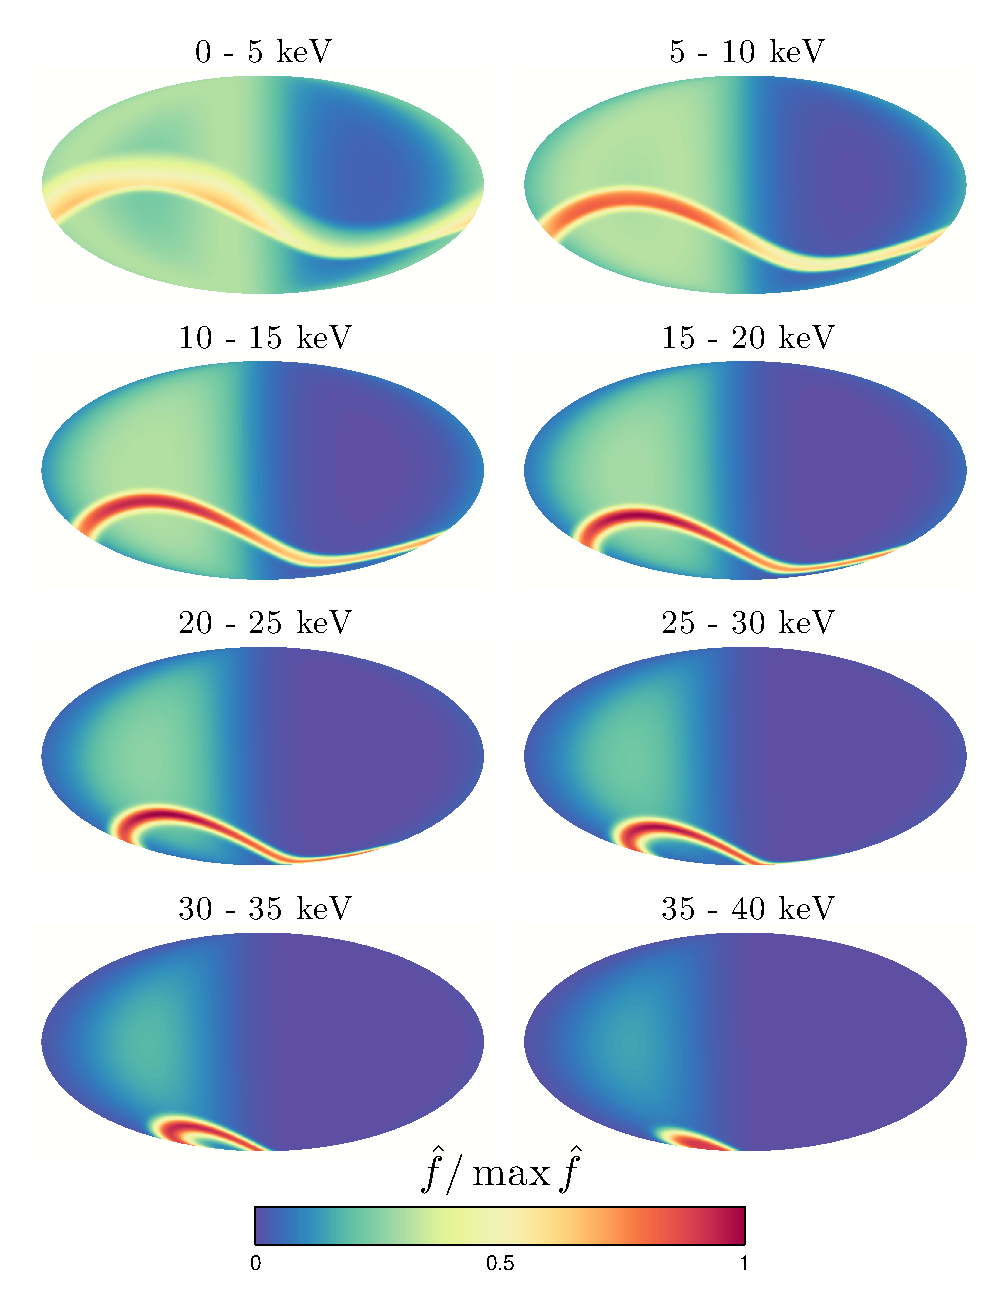
\includegraphics[trim = 0mm 0 0mm 0mm, clip, width=0.8\textwidth]{Figures/streamskymap.eps}
	\caption[Directional recoil skymaps for the SHM+Stream model]{Mollweide projection skymaps of the rescaled Radon transform integrated over 5 keV bins in energy. The recoil pattern corresponds to the SHM+Str velocity distribution where we use the example of the Sagittarius stream and a $m_\chi = 50$ GeV WIMP scattering off $^{19}$F.}
	\label{fig:streamskymap}
\end{figure}

The parameters used to describe the stream are $\xi_{\rm str}$, $\textbf{v}_\textrm{str}$ and $\sigma_\textrm{str}$. When describing the properties of the stream we will also often express its direction in terms of the angle between $\textbf{v}_\textrm{str}$ and $\textbf{v}_\textrm{lab}$,
\begin{equation}\label{eq:deltatheta}
      \Delta \theta = \cos^{-1}\left(\frac{\textbf{v}_\textrm{lab} \cdot \textbf{v}_\textrm{str}}{v_{\rm str} v_{\rm lab}}\right).
\end{equation}
Because of the azimuthal symmetry in the SHM+Str model about $\textbf{v}_{\rm lab}$, the number of events originating from the stream will only depend on the stream direction through this parameter. This angle we define using the Galactic frame descriptions of $\textbf{v}_\textrm{str}$ and $\textbf{v}_\textrm{lab}$.

Formally the question we wish to answer is; how many events are needed to reject at a given confidence level a smooth and isotropic halo in the case that the true distribution possesses an additional substructure component? In Fig.~\ref{fig:signal_comparison_skymap} the problem is displayed visually; how does one extract information about a stream from some set of spherical data collected over a short exposure? The left hand panels show the normalised directional signal observed in a perfect detector with infinite exposure, under the astrophysical parameters given in Table \ref{tab:partable}. The top two panels displaying the signal with no stream present, and the bottom after inclusion of the stream. The right hand panels show an example of the signal expected in a detector over an exposure of $\mathcal{E}=10$ kg yr, including the signal from isotropic experimental backgrounds. The data have been binned on a sphere using a HEALPix \cite{Gorski:2004by} equal angular area discretisation with 768 pixels. Statistical tests must be able to distinguish between these two types of signal. Whilst detecting the directionality of the signal thus confirming the Galactic origin of the scattering particle requires few events, confirming deviations from a smooth halo will require a larger number.

In most of the following results unless otherwise stated we fix to a single WIMP particle benchmark\footnote{At the time when this study was originally conducted this benchmark was not excluded by constraints from direct detection experiments but has since been excluded by PICO-60~\cite{Amole:2017dex}.}, namely a WIMP with a mass of $m_\chi = 50 \, \, \mathrm{GeV}$ and a solely SD WIMP-nucleon cross section of $\sigma^{\rm SD}_p = 10^{-39} \, \, \mathrm{cm}^2$. This is primarily for clarity in describing our results. We do of course expect our results to be dependent on this choice however we do not expect that varying it will be particularly insightful for understanding the working of our statistical tests. Our mock experiment is based on a $^{19}$F target, inspired by existing low pressure gas TPCs with CF$_4$ such as NEWAGE~\cite{Nakamura:2015iza,Miuchi:2010hn} and DMTPC~\cite{Leyton:2016nit}. For simplicity we neglect in all the results in this Chapter the time dependence of $\textbf{v}_{\rm lab}$ which is mostly unimportant for the event numbers we consider here. In the following Chapter we extend to a full direction+energy+time analysis.

\begin{figure}
    \centering
    %trim option's parameter order: left bottom right top
    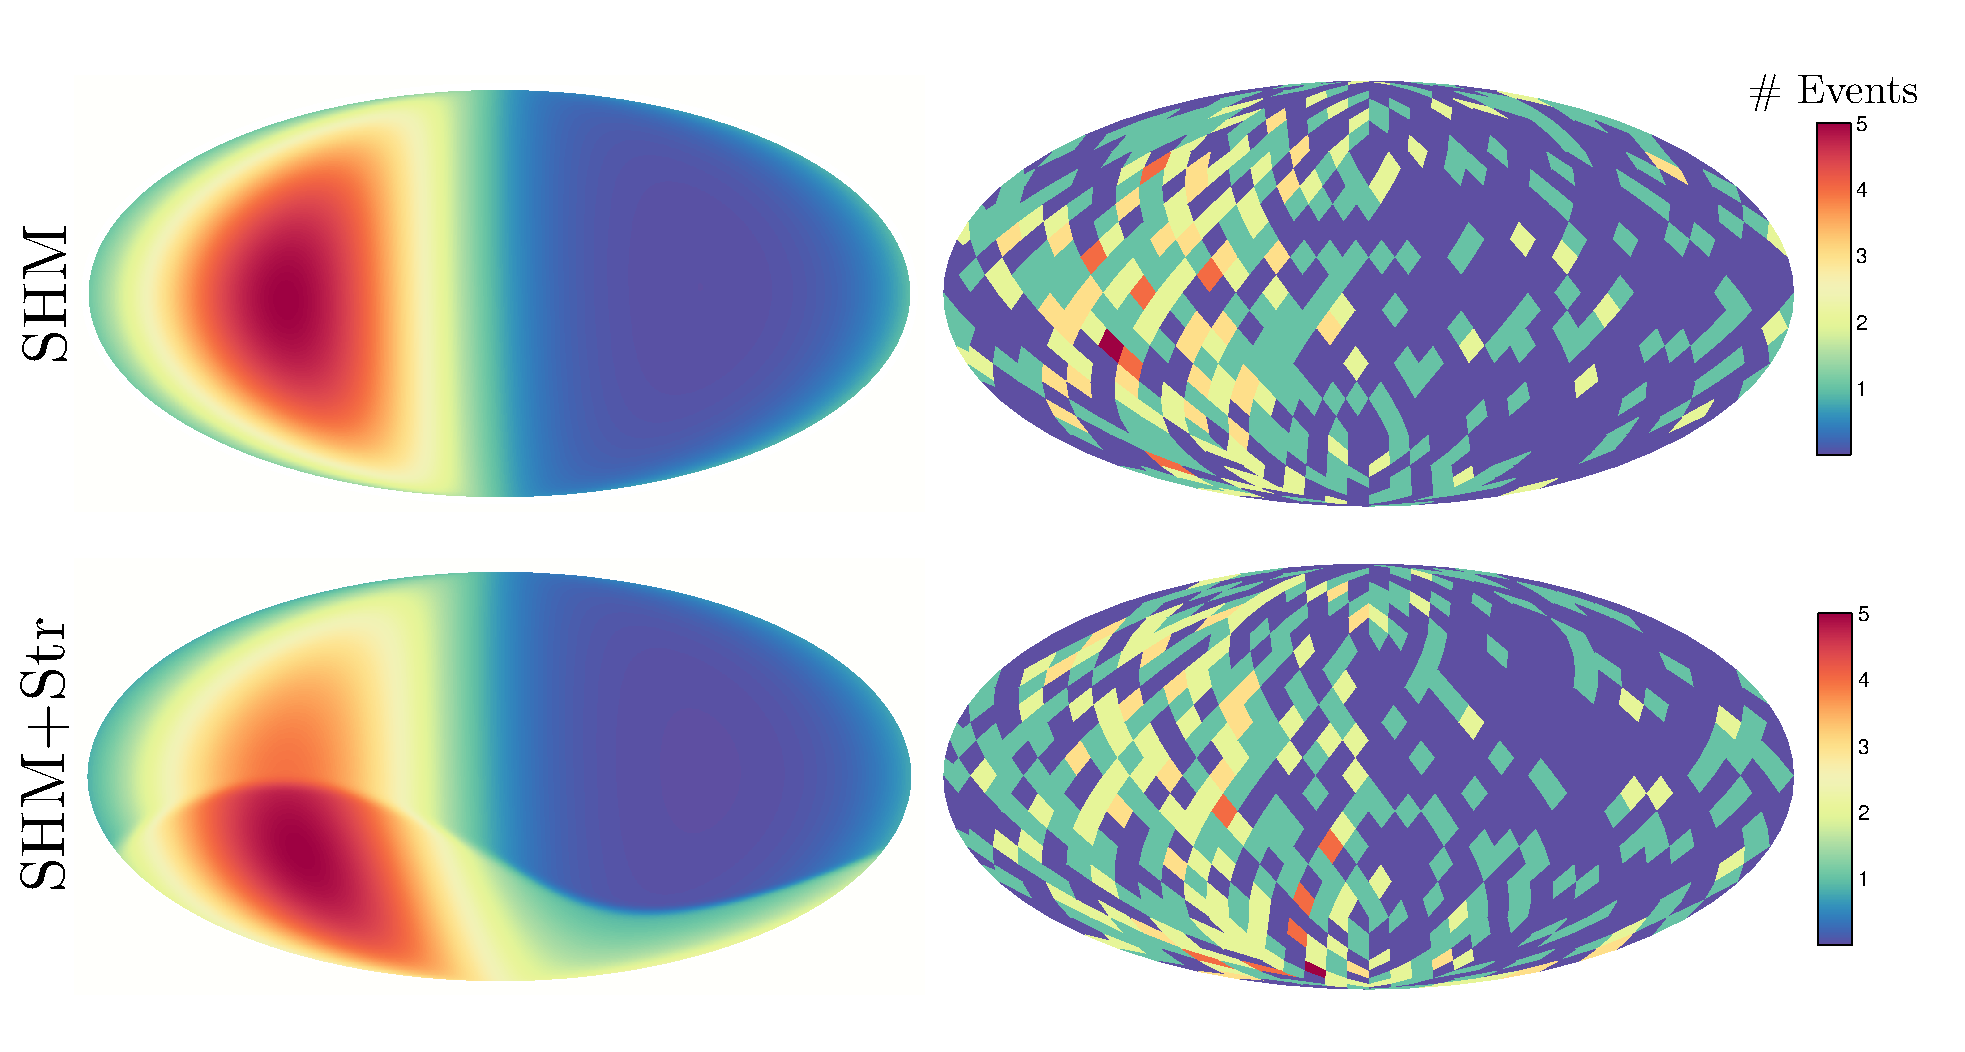
\includegraphics[trim = 0mm 0mm 0mm 0mm, clip, width=0.99\textwidth]{Figures/signal_comparison_skymap.eps}
    \caption[Simulated data for the SHM and SHM+Stream models]{SHM (top row) and SHM+Str (bottom row) direction-only signals for the underlying distribution (left column) and a set of data (right column) with an isotropic experimental background present. The signals are for a 50 GeV WIMP and astrophysical parameters from Table~\ref{tab:astrobenchmarks}. Our mock experiment uses a $^{19}$F target and in this case an energy sensitive window of $[5,100]$~keV. The datasets on the right are for a 10 kg yr exposure and a signal fraction of 0.5.}
    \label{fig:signal_comparison_skymap}
\end{figure}

\subsection{Non-parametric statistics}\label{sec:directional_nonparametric}
We can test for the presence of streams in the velocity distribution with statistics designed for spherical data. The general procedure involves first extracting some statistic $\mathcal{T}>0$ from the data that is distributed according to $p_0(\mathcal{T})$ under a null hypothesis (no stream present, $\xi_{\rm str}=0$) and $p_1(\mathcal{T})$ under an alternative hypothesis (stream present, $\xi_{\rm str}>0$). For some statistics these distributions may be known analytically but if not they can be built with a Monte Carlo simulation. For a particular result $\mathcal{T}_\textrm{obs}$ we define the `significance' to be the probability of measuring $\mathcal{T}<\mathcal{T}_\textrm{obs}$ if the null hypothesis is true,
\begin{equation}\label{eq:significance}
	S = \int_{0}^{\mathcal{T}_\textrm{obs}} p_0(\mathcal{T}) \textrm{d}\mathcal{T}.
\end{equation}   
We also define the statistical power as the probability of rejecting the null hypothesis if the alternative hypothesis is true. In other words it is the probability of measuring $\mathcal{T}>\mathcal{T}_\textrm{obs}$ in the alternative case,
\begin{equation}
	P = \int_{\mathcal{T}_\textrm{obs}}^{\infty} p_1(\mathcal{T})\textrm{d}\mathcal{T} \, .
\end{equation}
We build these two distributions from the repeated application of the statistical test on Monte Carlo generated Poisson datasets\footnote{For the details of the scattering simulation used to generate directional detection data see Appendix~\ref{app:scattering}.} for a particular set of input parameters. We then find the value of $\mathcal{T}$ for which $P=0.95$, i.e. the value achievable in 95\% of hypothetical experiments. Our results can then be expressed in units of $S_{95}$ calculated from $p_0$ at the same value of $\mathcal{T}$; $S_{95}$ is therefore the minimum detection significance achievable in 95\% of experiments.

There are two appropriate statistical procedures we can use to test for the existence of streams. The first test is a median direction test where the statistic follows a $\chi^2$ distribution for a set of data that has a median direction along some predicted direction. The second test is based on the modified Kuiper statistic, $V^\star$, and measures the degree to which a set of data has rotational symmetry about some predicted direction. In both cases we set the predicted direction satisfied by the null hypothesis to $\hat{\textbf{x}}_\textrm{lab}~=~-\textbf{v}_\textrm{lab}/v_{\rm lab}$. Details about the calculation of these test statistics can be found in Appendix~\ref{app:dirstats}.

\begin{figure}
      \centering
      %trim option's parameter order: left bottom right top
      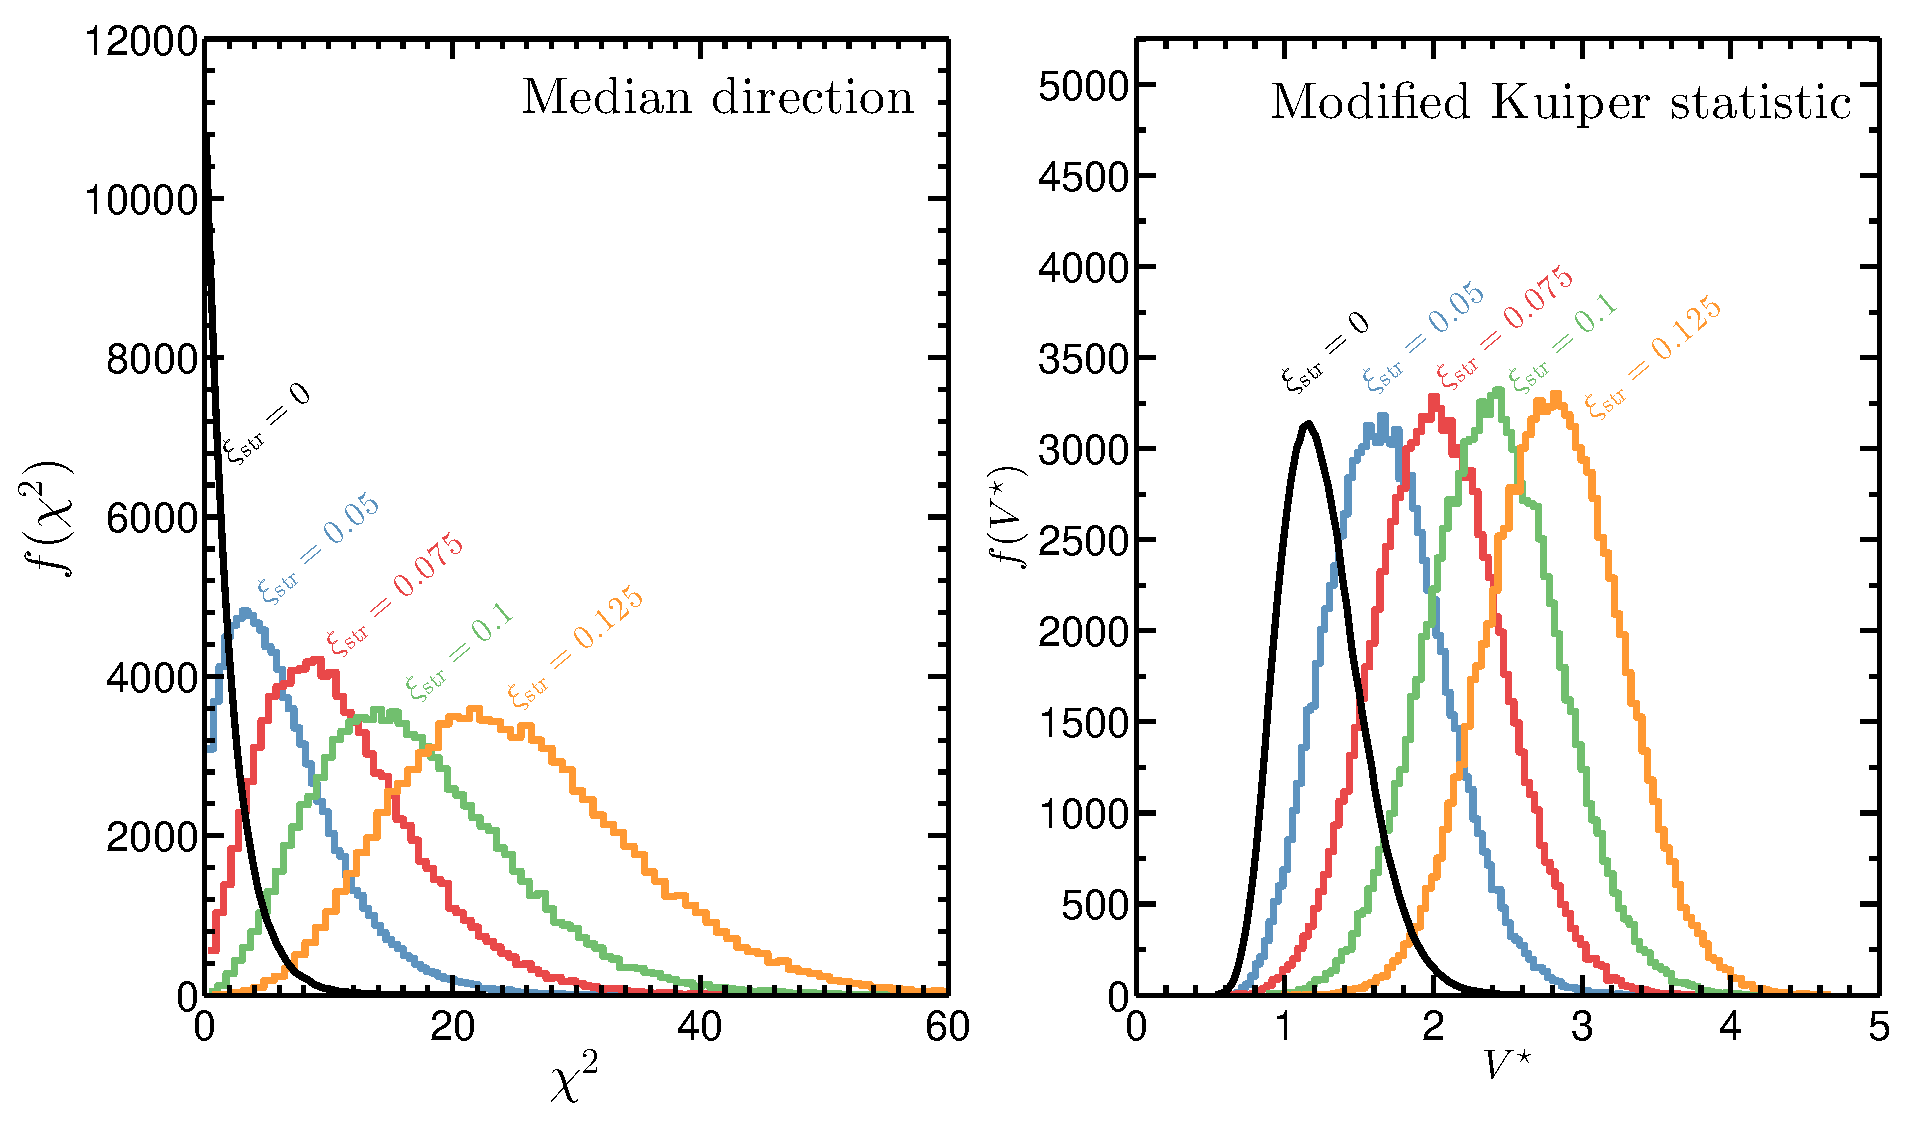
\includegraphics[trim = 0mm 0mm 0mm 0mm, clip, width=0.99\textwidth]{Figures/dirstatsdists.eps}
      \caption[Distributions of statistics for varying stream densities]{Distributions of the median direction $\chi^2$ statistic, and Kuiper statistic, $V^\star$,  built from $10^5$ Monte Carlo mock experiments. The distributions compare the case when there is no stream  present ($\xi_{\rm str} = 0$, black curve) and for streams of varying fractions ($\xi_{\rm str} > 0$, coloured histograms increasing left to right) cases.}
      \label{fig:dirstatsdists}
\end{figure}
Examples of the distributions of the statistics with a stream present as well as the distributions in the null case are shown in Fig.~\ref{fig:dirstatsdists}. The distributions in each case were generated from $10^5$ mock experiments with an exposure of $\mathcal{E} = 10$~kg~yr. As $\xi_{\rm str}$ is increased the signal becomes more influenced by the stream and hence the degree of rotational asymmetry is increased and the median direction becomes more displaced from $\hat{\textbf{x}}_\textrm{lab}$. We see this in the distributions of the statistics, for cases which disagree more with the null hypothesis, their distributions are further from the null distribution.

\begin{figure}
    \centering
    %trim option's parameter order: left bottom right top
    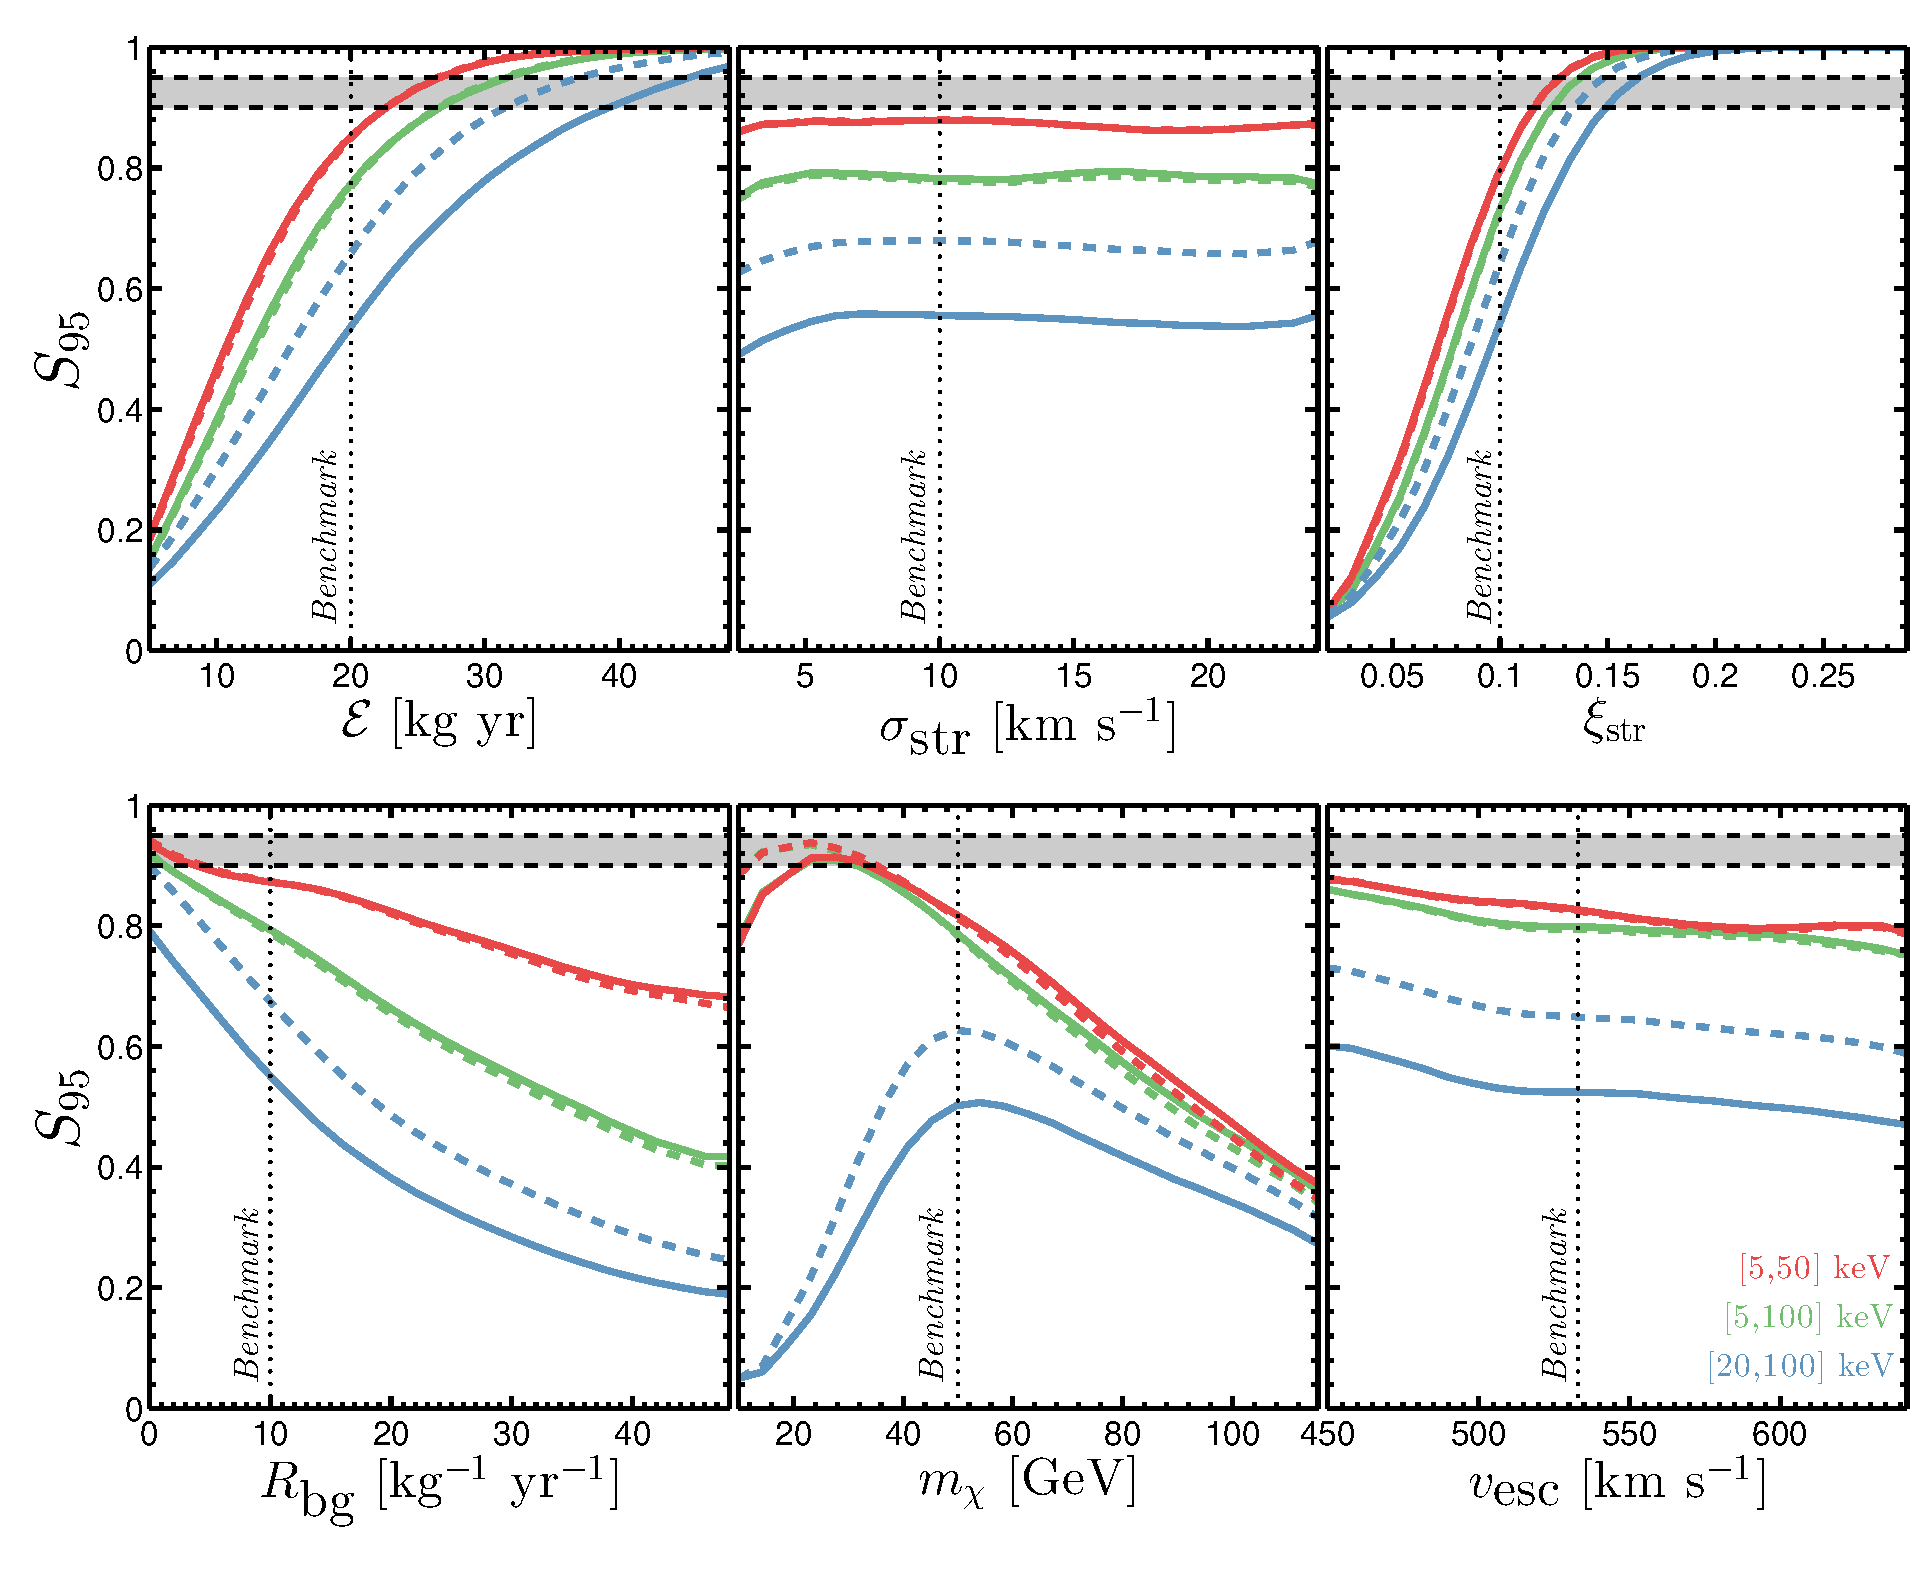
\includegraphics[trim = 0mm 0mm 0mm 0mm, clip, width=0.98\textwidth]{Figures/testcompare_sagit.eps}
    \caption[Results of non-parametric tests as a function of input parameters]{Significance obtainable by 95\% of experiments as a function of exposure, stream dispersion, stream density fraction, background rate, WIMP mass and escape speed for the Median direction (solid lines) and Kuiper (dashed lines) tests under the Sagittarius stream. The results are shown for energy windows of $[5,100]$ keV (green), $[5,50]$ keV (red) and $[20,100]$ keV (blue). The dashed lines indicate the desired $0.9-0.95$ level and the dotted lines in each plot indicate the input parameter used in the neighbouring plots.}
    \label{fig:testcompare_sagit}
\end{figure}
We first establish the role of the parameters other than the stream speed and direction on the performance of the tests; for now we focus on the benchmark case of the Sagittarius stream. In Fig.~\ref{fig:testcompare_sagit} we plot $S_{95}$ using the Kuiper and median direction $\chi^2$ tests. We show how this quantity varies with exposure time, stream dispersion, stream density, escape speed, WIMP mass and experimental background rate. As will become clear a choice that is particularly influential on our results here is the energy sensitive window of the detector, i.e. the threshold and maximum analysis energies. We display results for three examples, $[5,100]$ keV, $[5,50]$ keV and $[20,100]$ keV.

These first results are reasonably intuitive, with longer exposure times or for streams that takes up a larger fraction of the local DM density the signal is stronger and hence the tests perform better. The number of WIMP recoils from the stream scales linearly with exposure time and stream density fraction hence the significance of the result scales as roughly the square root of those quantities. Experiments with larger background rates perform predictably poorly compared to those with fewer backgrounds to contaminate the WIMP signal. Note that the quoted value of $R_\textrm{bg}$ is the rate observed in the case $[5,100]$ keV, the value taken for the other ranges has been scaled to account for the smaller sensitive window. The dispersion of the stream has no effect on the performance of the test, this is because of how the WIMPs scatter into the same angular area independent of how dispersed the distribution of their velocities is. To detect the Sagittarius stream at 90 - 95\% confidence in 95\% of experiments, one would need exposures between 10 - 20 kg yr for stream densities of around $\xi_{\rm str} \sim 0.1$, however this is lower for larger values of $\xi_{\rm str}$. The performance of the tests also depends on $m_\chi$, due mainly to the variation in the total number of events. Finally, the significance achieved decreases weakly as the escape speed is increased. This is because increasing $\vesc$ doesn't affect the recoils from stream, but slightly increases the number of recoils from the smooth halo scattering above the threshold.


\begin{figure}
	\centering
	%trim option's parameter order: left bottom right top
	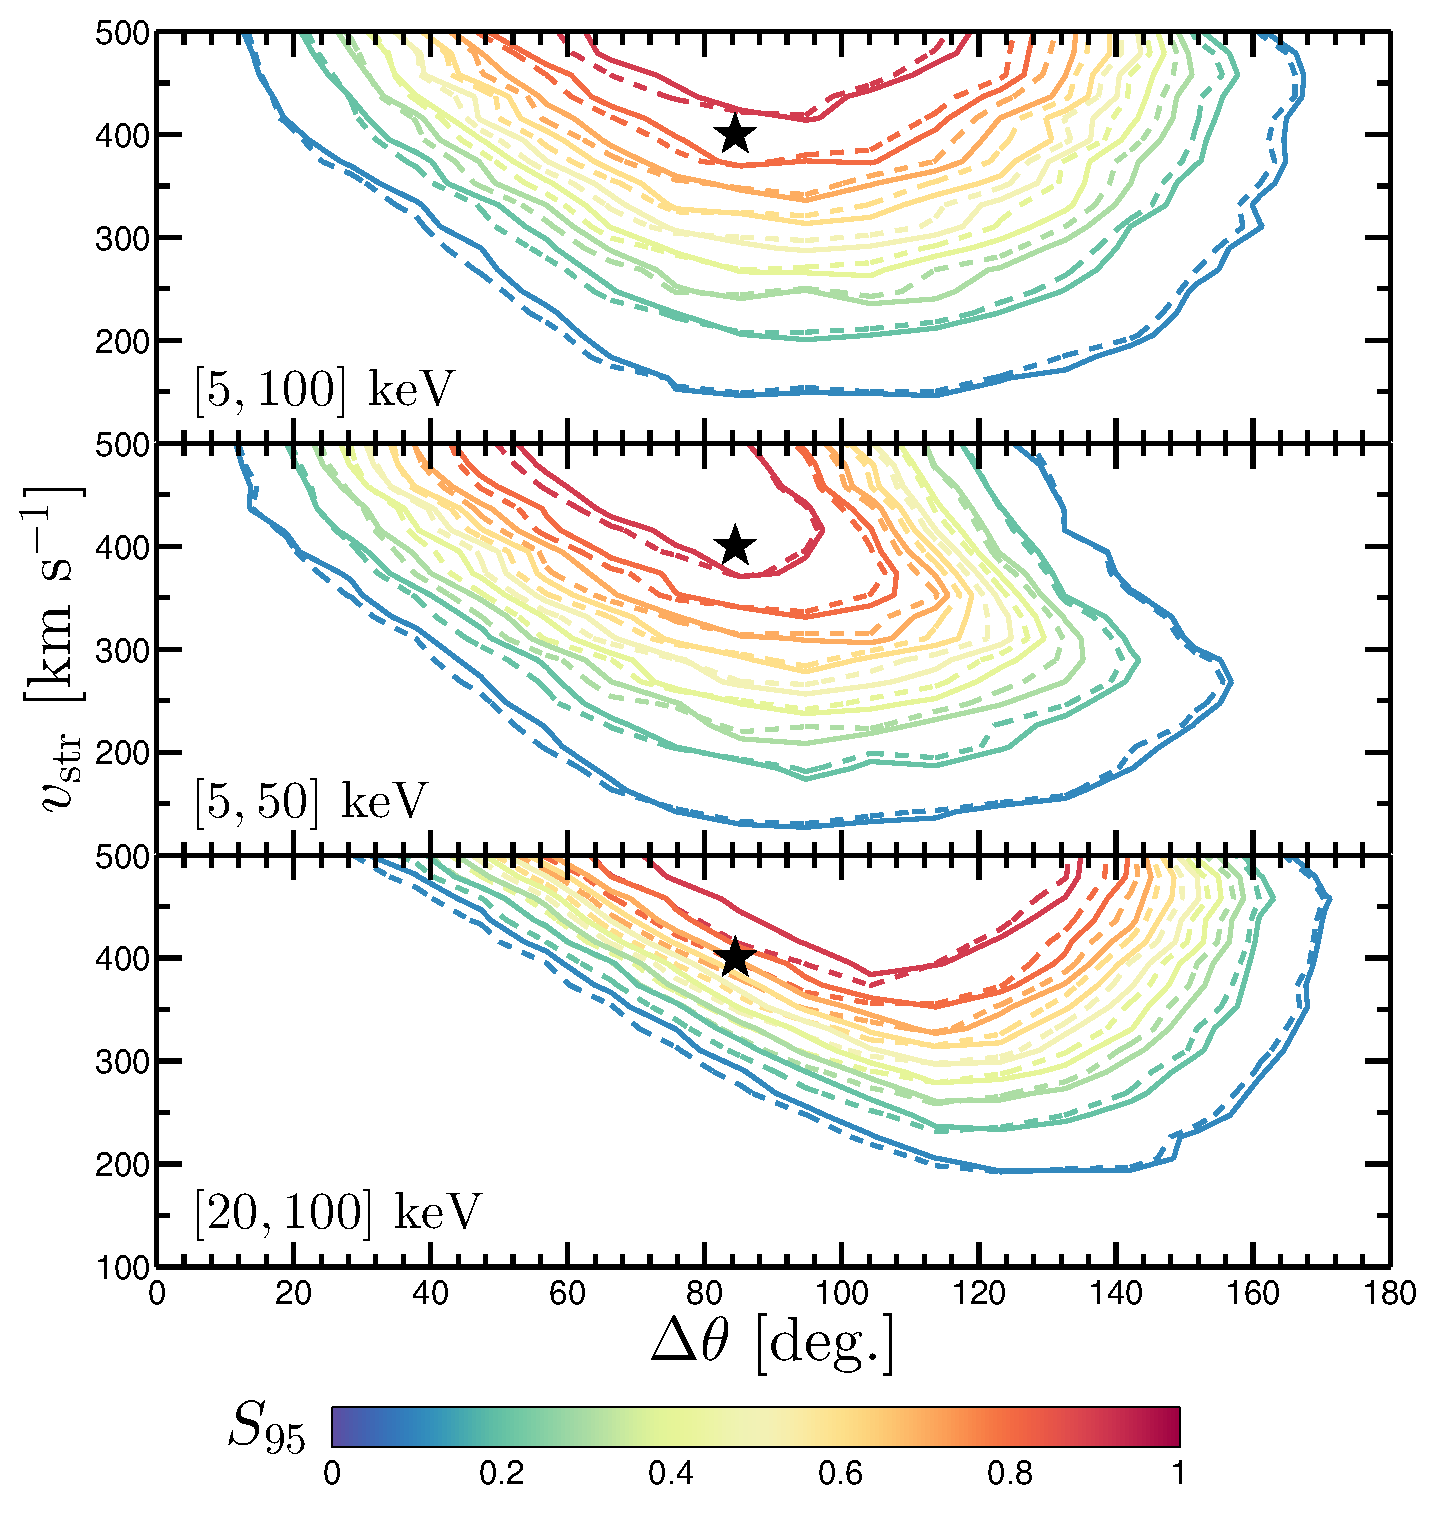
\includegraphics[trim = 0mm 0mm 0mm 0mm, clip, width=0.9\textwidth]{Figures/testcomparison_DeltaTheta_cont.eps}
	\caption[Non-parametric tests as a function of stream velocity]{Significance obtainable by 95\% of experiments over a 10 kg yr exposure as a function of stream speed and Galactic frame angle between stream direction and the lab velocity. The result for the Kuiper test is shown by the dashed lines and the median direction $\chi^2$ test by the solid lines. The three panels show the results for the three energy windows considered.}
	\label{fig:testcomparison_DeltaTheta}
\end{figure}
Having established the effect of the aforementioned parameter choices we will explore the detectability of general stream speeds and directions. For our results to be comprehensive the stream velocity need only be described by two parameters, the speed of the stream $v_\textrm{str}$ and the Galactic frame angle between the lab and stream velocities, $\Delta \theta$, defined in Eq.~(\ref{eq:deltatheta}). From symmetry arguments, changing the stream azimuthal angle with respect to $\textbf{v}_\textrm{lab}$ will not affect any of our results as it yields the same angular spectrum up to a rotation. Figure \ref{fig:testcomparison_DeltaTheta} shows how the significance varies with stream direction and speed, as well as the dependence on the energy window of the detector. The tests do not perform equally well over the range of stream directions. In particular the tests return a low significance when the stream is anti-aligned with the lab velocity as in this case the hypotheses of rotational symmetry and median direction are correct and the distribution of the statistics reverts to that of the null case. The other important contribution to the significance of the test result is from the number of observed stream recoils which for small $\Delta\theta$ is very low and for slower streams or high threshold energies as low as 0. The symmetry in the plots is due to this dependence on both the sample size and the positioning of the stream recoils with respect to the background halo recoils. One can also see that for the fastest streams, increasing the threshold energy results in a higher value of significance, this can be attributed to what is essentially a background rejection effect, whereby removing some of the low energy halo recoils the stream appears stronger in the signal, even with fewer overall events. The drop-off at large $\Delta\theta$ in the case of the 50 keV maximum energy is due to the stream recoils falling above the energy window, which is the reverse effect as at low values of $\Delta\theta$ in the case when the threshold has been increased to 20 keV.

A weakness of the Kuiper and median direction tests are that they exploit the direction information of the recoils only; the use of the recoil energy as well as the directional information is desirable. It may be possible to include the energy dependence of the signal by performing the test successively on energy ordered recoils or by binning the recoils in energy. In the case where there is no stream present the hypotheses of rotational symmetry and median direction are satisfied for all energies. However with a stream in the signal there will be a range of energies where the hypothesis is not satisfied. The degree to which the test is failed will increase for larger energies and then above a certain value of energy set by the stream speed, the test returns a value closer to the null case. Accounting for this effect in the test statistic would decrease the overlap between the null and alternative distributions and hence increase the significance of a particular result. However it is likely to be a small effect, as we showed in Fig~\ref{fig:polar}, the enhancement in the recoil energy spectrum induced by a stream is very slight. Furthermore dividing the recoils up in energy would result in a loss in information for each individual evaluation of the test statistic, so we expect the tests to perform on par or worse than without the energy information for low numbers of recoils. A more powerful method of including the energy dependence of the signal is with a likelihood fit.





\subsection{Likelihood analysis}\label{sec:directional_likelihood}
We turn our attention now towards a statistical test capable of placing constraints on the properties of the stream as well as testing for its existence. First we require a likelihood function. There are 11 free parameters in our model, $\boldsymbol{\theta} = \lbrace m_\chi, \sigma^{\rm SD}_p, \rho_0, \sigma_v,v_\textrm{esc},\sigma_\textrm{str},\textbf{v}_{\rm str},\xi_{\rm str},R_\textrm{bg}\rbrace$, where we split the velocity of the stream into its three Galactic coordinate components. We define the likelihood function as the product of the probabilities for obtaining recoils located at $(E_r^i,\hat{\textbf{q}}^i)$ ($i = 1, ..., N_{\rm obs}$) multiplied by a Poisson factor accounting for the probability of obtaining $N_{\rm obs}$ observed events given an expected number $N_{\rm exp}(\boldsymbol{\theta})$,

\begin{equation}
	\mathscr{L}(\boldsymbol{\theta})= \frac{N_{\rm exp}^{N_{\rm obs}}}{N_{\rm obs} !} e^{-N_{\rm exp}} \times\prod_{i=1}^{N_{\rm obs}} \bigg[\lambda P_\textrm{wimp}(E_r^i,\hat{\textbf{q}}^i) + (1-\lambda)P_\textrm{bg}(E_r^i)\bigg] \nonumber. 
\end{equation}
The expected number of events is a function of the parameters $\boldsymbol{\theta}$ and defined as, 
\begin{eqnarray}
	N_{\rm exp} &=& N_{\rm exp}^{\textrm{wimp}} + N_{\rm exp}^{\textrm{bg}} \\ &=& \mathcal{E} \left[ \int_{E_\textrm{th}}^{E_\textrm{max}} \int_{\Omega_r} \frac{\textrm{d}^2R}{\textrm{d}E_r \textrm{d}\Omega_r}\, \textrm{d}\Omega_r \, \textrm{d}E_r+ R_\textrm{bg}\right].
\end{eqnarray}
The probabilities $P_\textrm{wimp}$ and $P_\textrm{bg}$ are the probabilities for an event to occur at $(E_i,\hat{\textbf{q}}_i)$ in the signal and background (no WIMP) cases respectively, i.e.
\begin{eqnarray}
	P_\textrm{wimp}(E^i_r,\hat{\textbf{q}}^i; \boldsymbol{\theta}) &=& \frac{1}{R} \frac{\textrm{d}^2 R}{\textrm{d}E_r\textrm{d}\Omega_r}\bigg|_{E_r^i,\hat{\textbf{q}}^i; \boldsymbol{\theta}} \\
	P_\textrm{bg}(E_r^i) &=& \frac{1}{4\pi R_{\rm bg}} \frac{\textrm{d}R_{\rm bg}}{\textrm{d}E_r}.
\end{eqnarray}
The background probability  distribution we assume is isotropic with an exponentially falling recoil spectrum $\textrm{d}R_{\rm bg}/\textrm{d}E_r \propto \exp\left(-E_r/17.5\,{\rm keV}\right)$ where 17.5~keV is chosen to mimic the slope of the recoil energy spectrum of a 50 GeV WIMP in a fluorine experiment. We sum the signal and background distributions weighted by the signal fraction $\lambda$ defined as,
\begin{equation}
  \lambda = \frac{N_{\rm exp}^\textrm{wimp}}{N_{\rm exp}} \, .
\end{equation}
The parameter that will always be poorly recovered in this analysis is $v_\textrm{esc}$, as its effect on the recoil energy spectrum is very small and usually only becomes important at energies beyond the maximum set for directional detectors. We can overcome this issue by treating $v_\textrm{esc}$ as a nuisance parameter and account for its uncertainty by hand by including an additional term to the likelihood in the form of a Gaussian with mean and standard deviation of $v_\textrm{esc} = 533\, \pm \, 54$ km s$^{-1}$ \cite{Piffl:2013mla}. We then multiply the original likelihood by this Gaussian function.

The WIMP density, $\rho_0$, and cross section, $\sigma^{\rm SD}_p$, will also be problematic as they only control the amplitude of the recoil spectrum and hence only the number of events seen for a given exposure. Even for the rather large stream densities that we are considering here the difference between the number of events seen in the stream case compared with the null case is small. Moreover, the two parameters are degenerate with one another meaning there is no single set of values for $\rho_0$ and $\sigma^{\rm SD}_p$ that maximise the likelihood function in its current form. So we also adopt a Gaussian parameterisation for $\rho_0$ at the correct value. We choose a mean and standard deviation that reflect the current observational constraints on the local density, $\rho_0 = 0.3 \, \pm \, 0.1$ GeV cm$^{-3}$ \cite{Read:2014qva}.

\begin{figure}
	\centering
	%trim option's parameter order: left bottom right top
	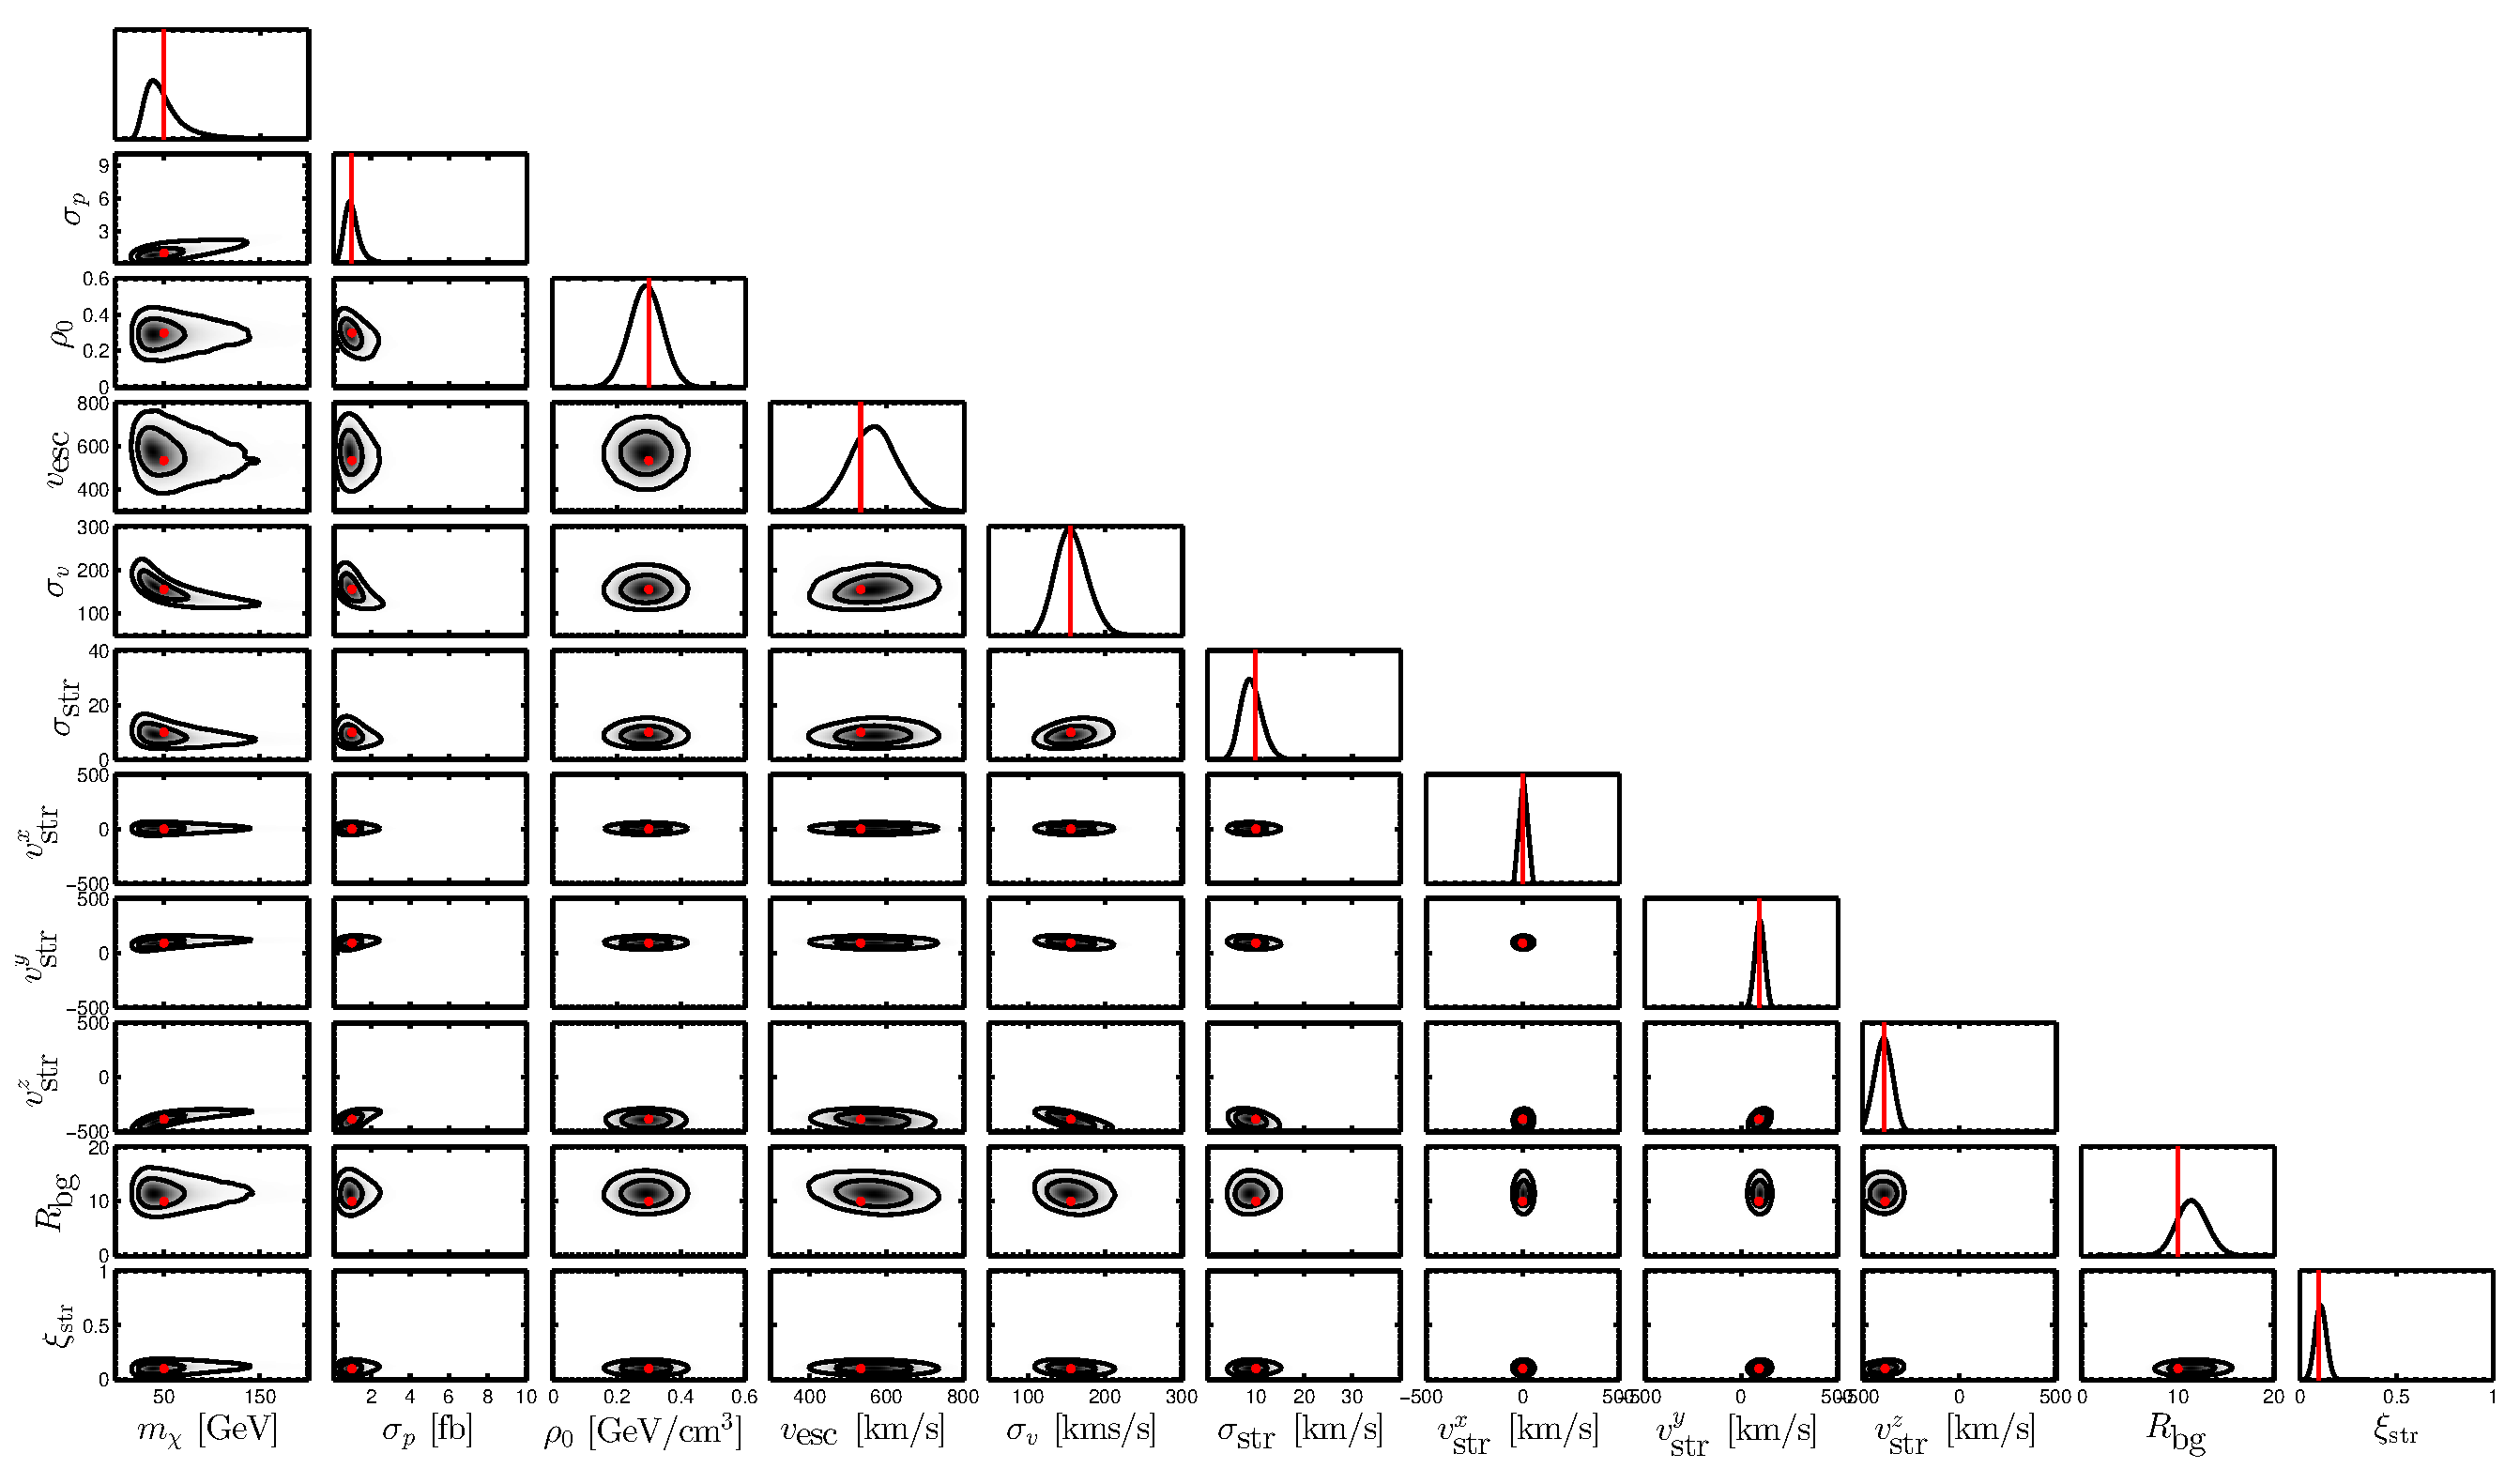
\includegraphics[trim = 0mm 0mm 0mm 0mm, clip, width=1.5\textwidth,angle=90]{Figures/posts_11params.eps}
	\caption[Triangle plot for reconstructed parameters of the SHM+Str model]{Triangle plot for reconstructed parameters of the SHM+Str model. The contours indicate the 68\% and 95\% confidence regions. The red dots/lines indicate the location of the input parameters.}
	\label{fig:posts_11params}
\end{figure}
First we will attempt to reconstruct the parameters of this model including the stream properties using the benchmark set of inputs. To do this we sample the likelihood over the full available parameter space with the nested sampling software \textsc{Multi}N\textsc{est} \cite{Feroz:2013hea, Feroz:2008xx} using 5000 live points, an evidence tolerance factor of 0.05 and sampling efficiency of 0.3. We then calculate 1-d (2-d) 68\% and 95\% confidence intervals (contours) using the asymptotic properties of the profile likelihood~\cite{Cowan:2010js}. The triangle plot of Fig.~\ref{fig:posts_11params} shows the parameter reconstructions in relation to the input values. The stream parameters, by virtue of being unconnected to the other halo parameters, are recovered well. The main source of uncertainty stems from the SHM and WIMP parameters, in particular $m_\chi$. The effect of the Gaussian parameterisation of $v_\textrm{esc}$ and $\rho_0$ is apparent and equivalent to using a Gaussian prior. There is a still some correlation in the $\rho_0-\sigma_p$ plane but the degeneracy has been broken. The halo parameters are reconstructed less accurately if they are not treated with a Gaussian function in the likelihood, however this parameterisation is representative of existing astrophysical measurements. This example shows that good constraints could be made on the parameters describing a stream if the correct model is used in constructing the likelihood function for the data. Importantly, we note that the exposure times needed to make these constraints  $\sim 5$ kg yr are significantly shorter than are needed when the non-parametric directional tests are used.

In analogy with the methodology of Sec.~\ref{sec:directional_nonparametric} we can use our likelihood function to develop a test for the existence of a stream in the data.  
An appropriate test involves the profile likelihood ratio statistic as it is based on the assumption that the null hypothesis is recovered by applying a constraint to a more general alternative hypothesis. A version of this test is often used to calculate WIMP discovery limits on the mass-cross section parameter space and will appear again in Chapter~\ref{chapter:nufloor}. Although here instead of testing for the presence of a WIMP over some background, rather we are testing for the existence of a stream in some already confirmed WIMP events.

We define the null hypothesis $H_0$ to be the SHM model and the alternative, $H_{\rm str}$, to be the SHM+Str model. The null hypothesis is then recovered with the same likelihood function under the constraint $\xi_{\rm str} = 0$. The likelihood ratio between the null and alternative hypotheses is,
\begin{equation}
	\Lambda = \frac{\mathscr{L}(\hat{\hat{\boldsymbol{\theta}}}, \xi_{\rm str} = 0)}{\mathscr{L}(\hat{\boldsymbol{\theta}} )} \, ,
\end{equation}
Where $\hat{\boldsymbol{\theta}}$ are the maximum likelihood estimators in the alternative model, and $\hat{\hat{\boldsymbol{\theta}}}$ are the maximum likelihood estimators evaluated when $\xi_{\rm str} = 0$. The likelihood ratio test statistic is then defined,
\begin{equation}
	\mathcal{D} = \left\{ \begin{array}{rl}
	-2\ln \Lambda  & \, \, 0\le \hat{\xi}\le1 \,,\\
	0  & \, \, \hat{\xi}<0, \, \, \hat{\xi}>1 \,.
	\end{array} \right. 
\end{equation}

Next we require a definition for the statistical significance of a particular test result. This requires knowledge of how the profile likelihood ratio test statistic $\mathcal{D}$ is distributed in the case that the null hypothesis is true, i.e. if the observed value is $\mathcal{D}_\textrm{obs}$
\begin{equation}
	S = \int_0^{\mathcal{D}_\textrm{obs}} f(\mathcal{D} | H_0) \, \textrm{d}\mathcal{D} \,.
\end{equation}
It is known however from Wilks' theorem \cite{Cowan:2010js} that the distribution of the profile likelihood ratio test statistic in the null case asymptotes towards a half $\chi_1^2$ distribution. Hence the discovery significance is defined as $S = \textrm{erf}\left(\sqrt{\mathcal{D}_\textrm{obs}/2}\right)$. However as we will be computing quite high values of significance it is simpler to deal in units of standard deviation, $\sigma$, i.e. $S = \sqrt{\mathcal{D}_\textrm{obs}}$. So a value of $\mathcal{D}_\textrm{obs} = 1$ corresponds to a 1$\sigma$ result or a significance of 68\%. The significance obtainable by 95\% of mock experiments, $S_{95}$, is then found by first building the distribution $f(\sqrt{\mathcal{D}})$ by applying the test on many Monte Carlo generated datasets containing a stream, and then solving the equation,
\begin{equation}
\int_0^{S_{95}} f(\sqrt{\mathcal{D}})\textrm{d}\sqrt{\mathcal{D}} = 0.95 \, .
\end{equation}

As in the previous Section, we demonstrate the performance of the test over a range of stream velocities where we again use the parameters $\Delta \theta$ and $v_\textrm{str}$ to describe the stream velocity. In Fig. \ref{fig:S95_DeltaTheta} we plot significance in units of $\sigma$ obtainable by 95\% of hypothetical experiments using the profile likelihood ratio test as a function of stream speed, $v_\textrm{str}$, and direction given by $\Delta \theta$, for the three energy windows considered. For comparison, in Fig. \ref{fig:N_wimp_str_location_cont} we plot the number of WIMPs originating in the stream, $N_\textrm{wimp}^\textrm{str}$, where we have split the observed events into stream and SHM recoils,
\begin{equation}
  N_\textrm{wimp} = N_\textrm{wimp}^\textrm{Str} + N_\textrm{wimp}^\textrm{SHM} \, .
\end{equation}

\begin{figure}
  \centering
  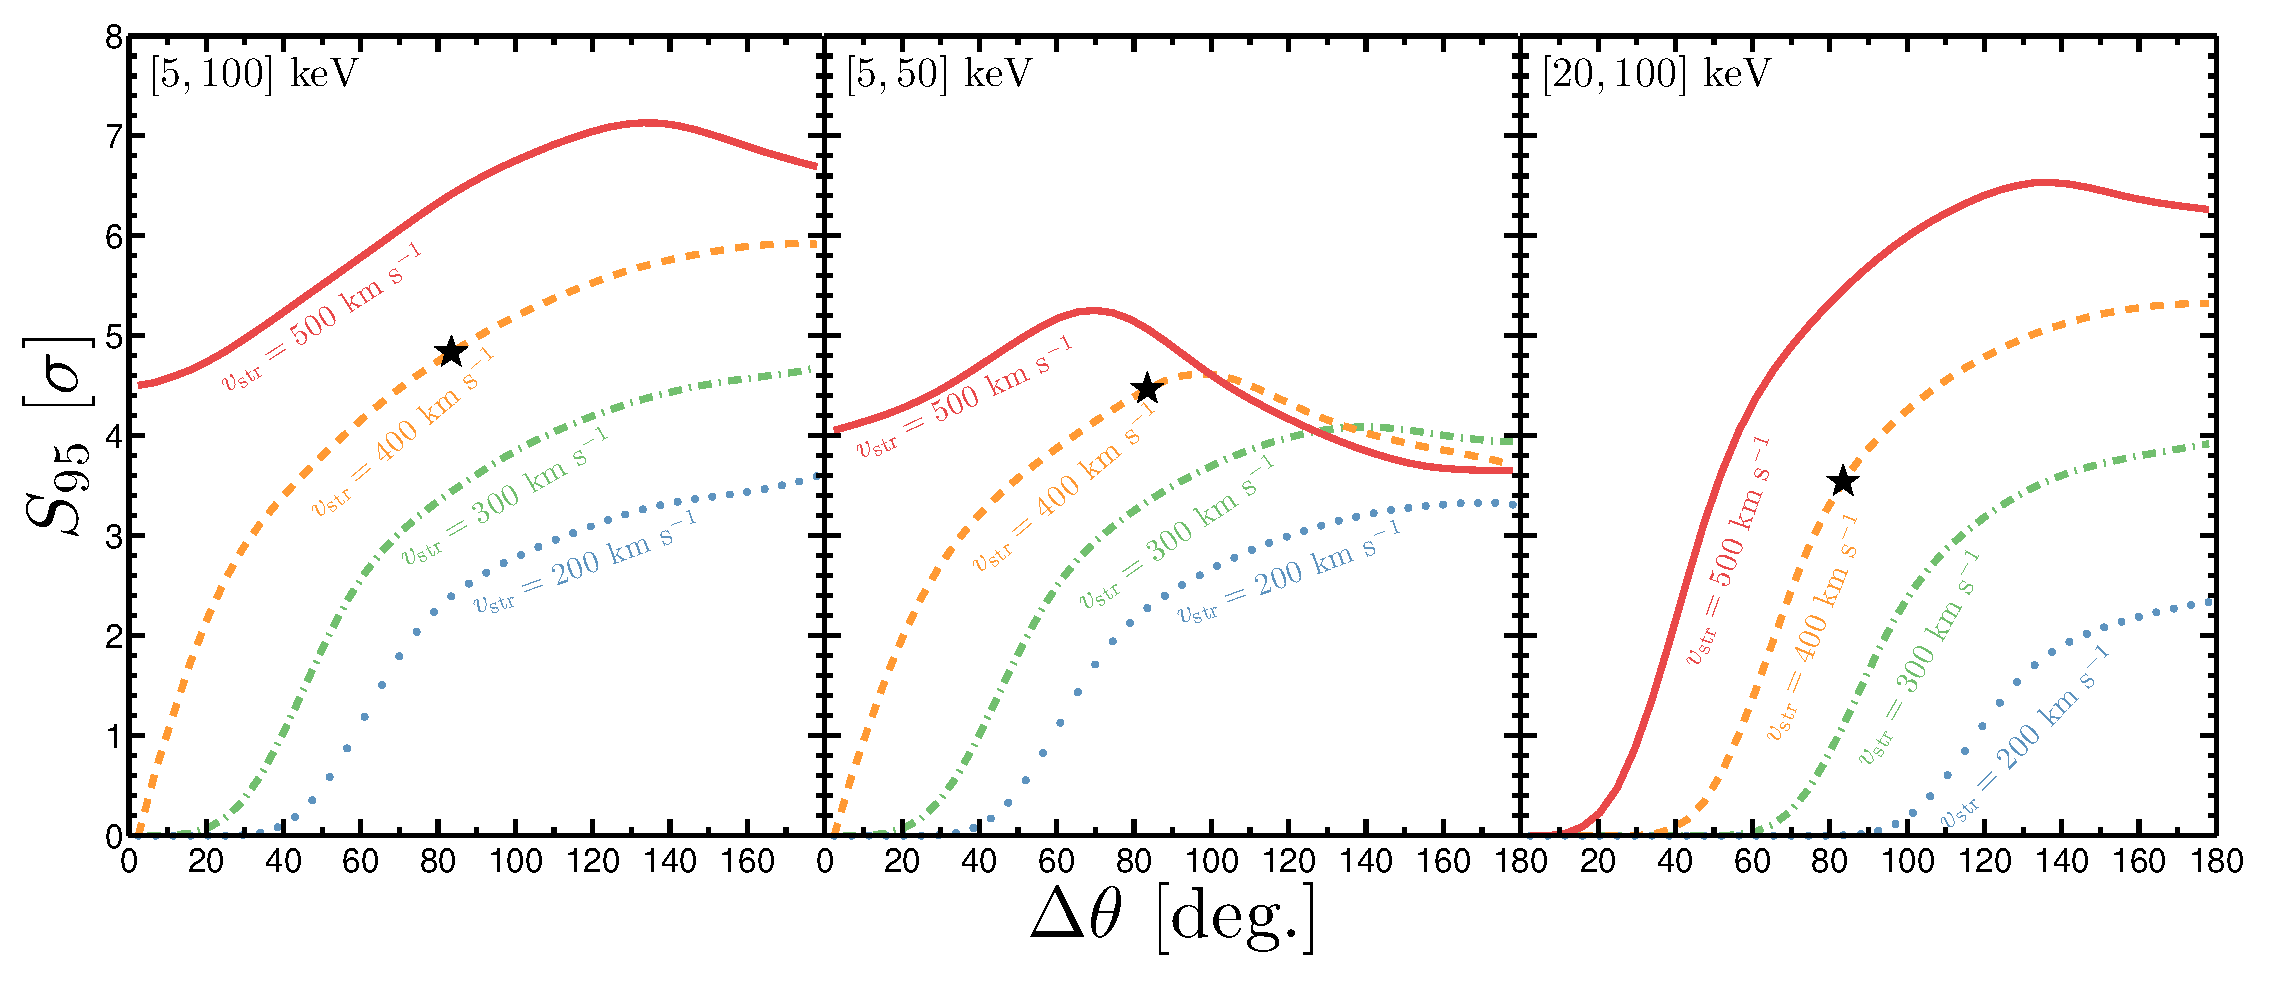
\includegraphics[trim = 0mm 0 0mm 0mm, clip, width=0.98\textwidth]{Figures/S95_DeltaTheta.eps}
  \caption[Profile likelihood test significance as a function of stream angle]{Significance achievable in 95\% of experiments in units of $\sigma$ using a profile likelihood ratio test. The test result is shown as a function of angle between lab and stream velocities. The curves correspond to, from top to bottom, $v_\textrm{str} = 500$ km s$^{-1}$ (red solid line), 400 km s$^{-1}$ (orange dashed), 300 km s$^{-1}$ (green dot-dashed), and 200 km s$^{-1}$ (blue dotted). The speed and direction of the Sagittarius stream example is indicated with a black star.}
  \label{fig:S95_DeltaTheta}
\end{figure}
\begin{figure}
  \centering
  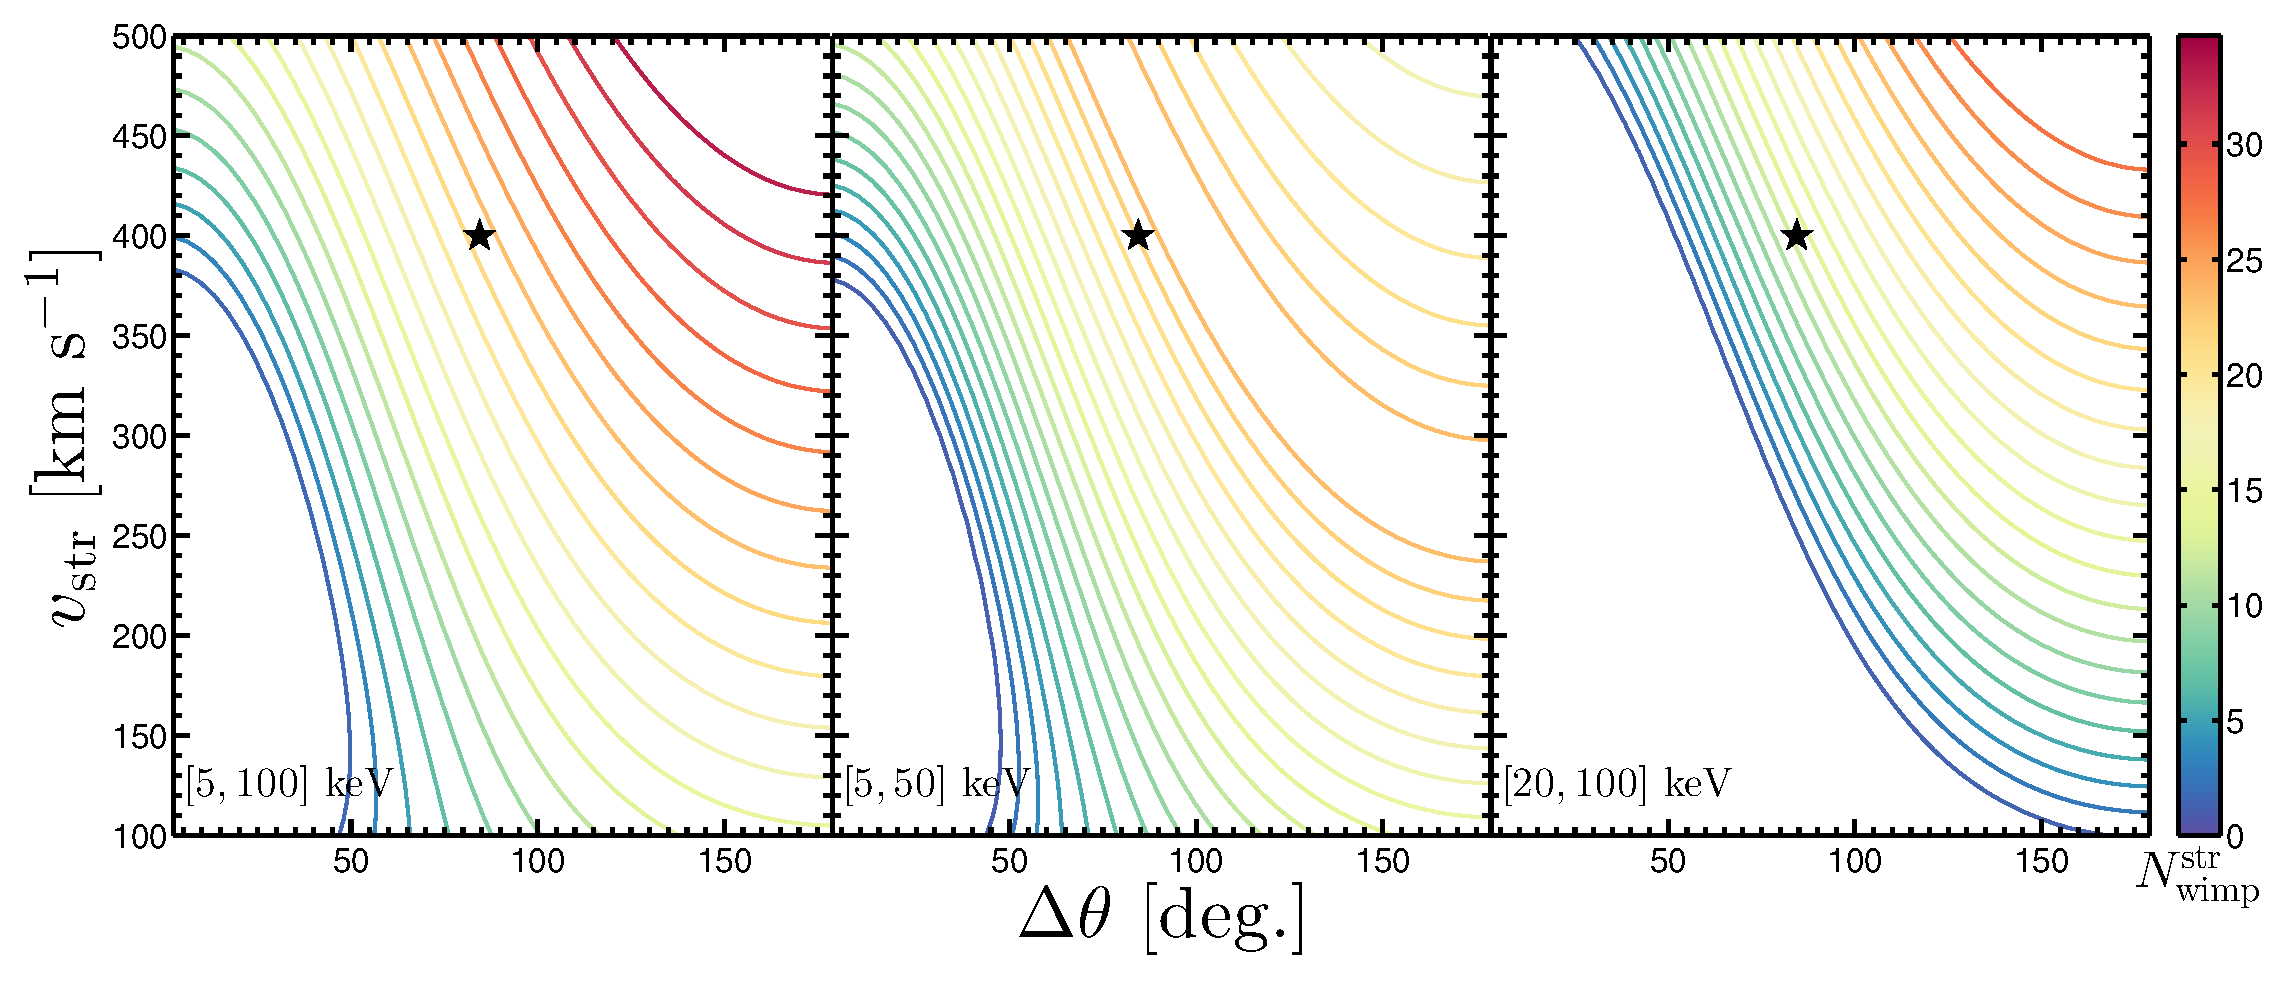
\includegraphics[trim = 0mm 0 0mm 0mm, clip, width=0.98\textwidth]{Figures/N_wimp_str_location_cont.eps}
  \caption[Number of stream recoils as a function of stream velocity]{Number of stream recoils as a function of stream speed, direction and for three energy sensitive windows (left to right panels). The speed and direction of the Sagittarius stream example is indicated with a black star.}
  \label{fig:N_wimp_str_location_cont}
\end{figure}
In Figs.~\ref{fig:S95_DeltaTheta} and \ref{fig:N_wimp_str_location_cont} the parameter values not displayed are fixed at the benchmark values used in Fig.~\ref{fig:testcompare_sagit}, with the exception of exposure which we now reduce to 5~kg~yr. The tests by virtue of being parametric perform much more powerfully than the non-parametric tests. The enhancement in performance can also be attributed to the use of the full energy and direction data whereas before only the direction information was used. Furthermore the tests achieve high significance over a wide range of stream velocities, with the limiting factor being the number of WIMPs coming from the stream, $N_\textrm{wimp}^{\textrm{str}}$, as can be seen by comparing the two Figures. For low values of $\Delta\theta$ when the number of stream WIMPs drops to 0, the significance can be seen to do likewise. There is similarly a dependence on the energy window of the detector which causes a reduction in the number of stream WIMPs when a portion of the stream recoils are excluded by the maximum of the energy window. This can be seen in the middle panels when the curves begin to decrease for large $\Delta \theta$. However the significance for faster stream speeds is enhanced over what might be expected simply from looking at $N_\textrm{wimp}^\textrm{str}$. This can be attributed to faster streams becoming more prominent in the signal due to the exponential drop off with energy of the event rate for the background halo.

\subsection{Discussion}
Using both non-parametric directional tests and a profile likelihood test, we have shown that there are reasonable prospects for the detection of a moderately high density tidal stream by a future directional detector. We began with the fixed example of a Sagittarius-like stream and then explored the dependence on the parameters of the stream, namely its speed, direction, dispersion and density. Using non-parametric directional statistics the detection of a Sagittarius-like stream would need a total of around 900 events, but with a likelihood fit good constraints can be placed on the stream parameters with around 300 events.

The advantage of using non-parametric tests is that one need not assume a model to describe the data, simply that the data satisfy either a null or alternative hypothesis. The advantage of the tests we exploit here is that they are constructed rather generally and the basic hypotheses are relatively simple. However non-parametric tests will always return a less significant result than parametric tests. The likelihood analyses also make use of both the energy and direction information of the recoils whereas the non-parametric tests are direction only. The disadvantage of the likelihood approach however is that we must pick a specific model to describe the substructure that one predicts to be present in the data. We now explore possible ways of making claims about the presence of non-Maxwellian structure in the halo in a parametric way that does not require particular choices for the functional form describing it.

\section{Reconstructing the velocity distribution}\label{sec:directional_reconstruction}
We now move to more model independent methods for measuring properties of the local velocity distribution. This will involve extending a general parameterisation of the {\it speed} distribution used in the analysis of standard direct detection data~\cite{Peter:2011eu,Kavanagh:2013wba}, to the fitting of the {\it velocity} distribution with directional data. There have been long-standing attempts to devise methodologies for handling astrophysical uncertainties in direct detection experiments, see e.g. Refs.~\cite{Fox:2010bz,Fox:2010bu,Frandsen:2011gi,Gondolo:2012rs,DelNobile:2013cta,Fox:2014kua,Feldstein:2014gza,Anderson:2015xaa,Gelmini:2016pei,Kahlhoefer:2016eds}. In the context of directional detection experiments the situation is more complicated as the angular recoil spectrum is much more sensitive to the values of the underlying astrophysical parameters. One must also consider the full 3-dimensional velocity distribution rather than the 1-d speed distribution and as such requires a suitable angular basis for the parameterisation. Past attempts to develop astrophysics independent methods for directional detection have involved decomposing the velocity distribution into integrals of motion~\cite{Alves:2012ay}, or spherical harmonics~\cite{Lee:2014cpa}.

Following the formalism introduced in Ref.~\cite{Kavanagh:2015aqa} we test a discretised approach for empirically parameterising the velocity distribution. The velocity distribution is divided into angular bins, each described by an empirical 1-d speed distribution which does not vary with angle over the bin. The goal now is to use mock data and likelihood fits to test the accuracy of the reconstructed WIMP signal using this empirical method compared with model-dependent fits. We also consider both energy only and directionally sensitive direct detection experiments to quantify the advantages of introducing angular information. We compare reconstructions of the WIMP mass, cross section and velocity distribution in three distinct cases: A) when the velocity distribution is known exactly; B) when the general functional form of the distribution is known (as in the previous Section); and C) when no assumptions are made about the velocity distribution. We test these three methods on the three benchmark velocity distributions defined in Chapter~\ref{chapter:direct}, the SHM, the SHM+Stream and the SHM+Debris Flow. 

As before we continue to fix our results at a single particle physics benchmark with a mass of $m_\chi = 50 \, \, \mathrm{GeV}$ and a solely SD cross section of $\sigma^{\rm SD}_p = 10^{-39} \, \, \mathrm{cm}^2$. We extend beyond the experimental setup introduced before to the combination of two experiments with xenon and fluorine targets. This allows us to explore the complementarity of multiple targets but also allows us finer control in the level of directional information used. We will consider cases in which neither experiment has directional sensitivity, in which only one of the experiments has directional sensitivity and in which both experiments are directionally sensitive. 

Our choice of a xenon target detector is inspired by projections for the next generation of ton-scale liquid xenon experiment such as LZ~\cite{Akerib:2015cja} and Xenon1T~\cite{Aprile:2015uzo}. Although these experiments are not designed with any directional sensitivity they represent a useful and realistic benchmark for an exposure and threshold ($\sim 5\,\textrm{keV}$) that can be expected in the next generation of direct detection experiments. Though as we discussed earlier there are tentative suggestions that it may be possible to extract directional information in liquid xenon experiments with columnar recombination~\cite{Nygren:2013nda,MuAaoz:2014uxa,Li:2015zga,Mohlabeng:2015efa}. The choice of a fluorine detector is the same as in the previous Section, inspired by existing low pressure gas TPCs with CF$_4$. For these results we set a modest threshold of 20 keV, in line with what is currently achievable~\cite{Leyton:2016nit}. A summary of the parameters used for each experiment and the number of events observed for each halo model are given in Table~\ref{tab:benchmarks}. 


\begin{table}[t]\centering
\ra{1.3}
\begin{tabularx}{\textwidth}{c|YYY|YYY}
\hline\hline
Target	& $E_\mathrm{th}$/keV	& $E_\mathrm{max}$/keV & $\mathcal{E}$/kg yr & $N_\mathrm{events}^{\mathrm{SHM}}$ & $N_\mathrm{events}^{\mathrm{SHM+Str}}$& $N_\mathrm{events}^{\mathrm{SHM+DF}}$ \\
\hline
Xe & 5 & 50 & 1000 & 878 & 922 & 893 \\
F   & 20 & 50 & 10 & 50 & 67 & 64 \\
\hline \hline
\end{tabularx}
\caption[Parameters for the two mock experiments]{Parameters for the two mock experiments considered in this Section: threshold energy $E_\mathrm{th}$, maximum analysis energy $E_\mathrm{max}$ and exposure $\mathcal{E}$. Also shown are the number of expected events in the both experiments for each of the three astrophysical benchmark models.}
\label{tab:benchmarks}
\end{table}

We compare the reconstruction of the WIMP and velocity distribution parameters made using three methods each with a different level of a priori knowledge assumed.
\begin{itemize}
\item{{\bf Method A: Perfect knowledge.} This is the best case scenario when both the functional form and parameter values of the velocity distribution are known exactly. The parameters that are reconstructed with this method are only $\{m_\chi,\sigma_p^{\textrm{SD}}\}$ for all three halo models.}

\item{{\bf Method B: Functional form known.} In this case the functional form of the velocity distribution (i.e. SHM, SHM+Str or SHM+DF) is known, however the parameter values are not. The number of parameters reconstructed with this method varies depending on the chosen halo model. In the case of the SHM there are 4 parameters: $\{m_\chi,\sigma_p^{\textrm{SD}},v_0,\sigma_v\}$. For the SHM+Str model (in a slight simplification from Sec.~\ref{sec:directional_nonparametric}) there are 9 parameters: $\{m_\chi,\sigma_p^{\textrm{SD}},v_0,\sigma_v,\sigma_{\rm str},\mathbf{v}_{\rm str},\xi_{\rm str}\}$, and for the SHM+DF model there are 6 parameters: $\{m_\chi,\sigma_p^{\textrm{SD}},v_0,\sigma_v,v_f,\xi_{\rm DF}\}$.}

\item{{\bf Method C: Empirical parameterisation.} With this method no knowledge is assumed about the form or parameters of the underlying velocity distribution. We fit the data using a discretised velocity distribution with three angular bins. This method is described in more detail below. Three parameters are used to describe the speed distribution within each angular bin, for a total of 11 parameters: $\{ m_\chi, \sigma_p^{\textrm{SD}}, a_0^{(k=1)}, a_1^{(k=1)}, \ldots, a_2^{(k=3)}, a_3^{(k=3)} \}$.} Each of the $a_m^{(k)}$ parameters (defined in the following subsection) is sampled linearly in the range $[-20, 20]$.
\end{itemize}


\subsection{Empirical parameterisation}\label{sec:directional_parameterisation}
To perform the model-independent reconstruction (Method C), we discretise the velocity distribution into $N$ angular bins, assuming that $f(\mathbf{v})$ has no angular dependence within each bin. As discussed in Ref.~\cite{Kavanagh:2015aqa}, using only $N=2$ angular components does not sufficiently capture the directionality of typical velocity distributions. We therefore use $N=3$ angular bins, such that the approximate velocity distribution can be written:
\begin{equation}\label{eq:discretisedf}
f(\textbf{v}) = f(v, \cos\theta, \phi) =
\begin{cases}
f^1(v) & \textrm{ for } \theta \in \left[ 0, \frac{\pi}{3}\right]\,, \\
f^2(v) & \textrm{ for } \theta \in \left[ \frac{\pi}{3}, \frac{2\pi}{3}\right]\,, \\
f^3(v) & \textrm{ for } \theta \in \left[ \frac{2\pi}{3}, \pi\right]\,. \\
\end{cases}
\end{equation}
We align the angular bins such that $\theta = 0$ (the `forward' direction) points along $\mathbf{v}_{\rm lab}$, anticipating that the greatest anisotropy in the velocity distribution will be generated by the motion of the Earth through the halo. The advantage of a discretised velocity distribution is that provided a suitable parameterisation for each $f^k(v)$ is chosen then the complete $f(\textbf{v})$ can be ensured to be everywhere positive, properly normalised and does not require any assumptions about the equilibrium conditions of the Milky Way halo. These issues are often not addressed by other attempts to describe $f(\mathbf{v})$~\cite{Alves:2012ay,Lee:2014cpa}.

Within each bin, we follow Ref.~\cite{Kavanagh:2013wba} and describe the 1-d (directionally averaged) velocity distributions using the following empirical parameterisation,
\begin{equation}\label{eq:polynomialparam}
f^k(v) = \exp \left[ - \sum_{m = 0}^3 a_m^{(k)} P_m(2v/v_\mathrm{max} - 1)\right]\,.
\end{equation}
Here, $P_m$ is the $m$th Chebyshev polynomial of the first kind. A value of $v_\mathrm{max} = 1000 \kms$ is chosen as a conservative cut-off for the velocity distribution. The shape of the velocity distribution within each bin is controlled by the parameters $\{a_m^{(k)}\}$. The values of $a_0^{(k)}$ are fixed by requiring that $f^k(0)$ is the same for all $k$ (i.e.~that the three distributions are consistent towards $\mathbf{v} = 0$). Finally, we rescale each of the $a_0^{(k)}$ to ensure that the full distribution is normalised to unity. This leaves us with three parameters in each of the $N=3$ angular bins.

When fitting the parameters of this empirical distribution, we do not keep all of the directional information for each event but instead bin the data into three angular bins (the same angular bins as defined in Eq.~(\ref{eq:discretisedf}), but with $\theta$ now referring to the \textit{recoil} angle with respect to $\mathbf{v}_{\rm lab}$). The expected recoil spectrum (as a function of $E_r$) is calculated by integrating the Radon Transform $\hat{f}(v_\mathrm{min}, \hat{\mathbf{q}})$ over the relevant angular range. For example, in the $j$th angular recoil bin, the differential rate of recoils (as a function of energy) is proportional to:
\begin{equation}
\label{eq:discreteRadon}
\hat{f}^j(v_\textrm{min}) = \int_{\phi = 0}^{2\pi} \int_{\cos(j\pi/N)}^{\cos((j-1)\pi/N)} \hat{f}(v_\textrm{min}, \hat{\textbf{q}})\, \mathrm{d}\cos\theta\,\mathrm{d}\phi\,,
\end{equation}
where $\theta$ and $\phi$ now refer to the direction of the recoil.

There are two reasons for this binning of the data. First, the full Radon Transform of this coarsely discretised distribution is unlikely to give a good fit to the distribution of recoil directions on an event-by-event basis. Instead, if we bin recoils on a similar angular scale, this should eliminate any spurious features in the directional spectrum and help mitigate the error induced by using a discretised approximation for the velocity distribution.

\subsection{WIMP mass and cross section}\label{sec:directional_mass}
We now present the reconstructed intervals for the particle physics parameters $m_\chi$ and $\sigma_p^\mathrm{SD}$. Firstly in the left panel of Fig.~\ref{fig:mx-recon}, we compare the reconstruction of the WIMP mass using each of the three approaches. In the best case scenario (Method A) when the velocity distribution is known exactly, the WIMP mass is reconstructed with high accuracy, obtaining best fit values with less than 2\% deviation from the input value of $m_\chi = 50 \,\,\mathrm{GeV}$. Generally with less assumed knowledge the error on the reconstructed mass is larger. However in the case of the SHM the constraints are wider in Method B than in Method C. This is likely due to the small (4-dimensional) parameter space used to reconstruct the SHM. The greater freedom in the (11-dimensional) empirical parameterisation (Method C) may allow for a better fit to the data in the presence of Poisson noise, leading to tighter constraints. For the SHM+Str and SHM+DF models, the underlying velocity distributions are more complex and the parameter space is much larger (9 and 6 dimensions respectively). In these models, the known functional form of Method B can fit the data closely. The empirical parameterisation instead explores a wide range of the parameter space, but cannot resolve the fine-grained features of these models, leading to wider uncertainties. We note that using each of the three methods, the true value of the WIMP mass lies within the 68\% confidence interval in all cases. The best fit masses reconstructed using Methods B and C are typically close in value, indicating that there is little bias induced in using the empirical parameterisation, despite the fact that we have assumed very little about the shape of the underlying distribution.

\begin{figure}
\centering
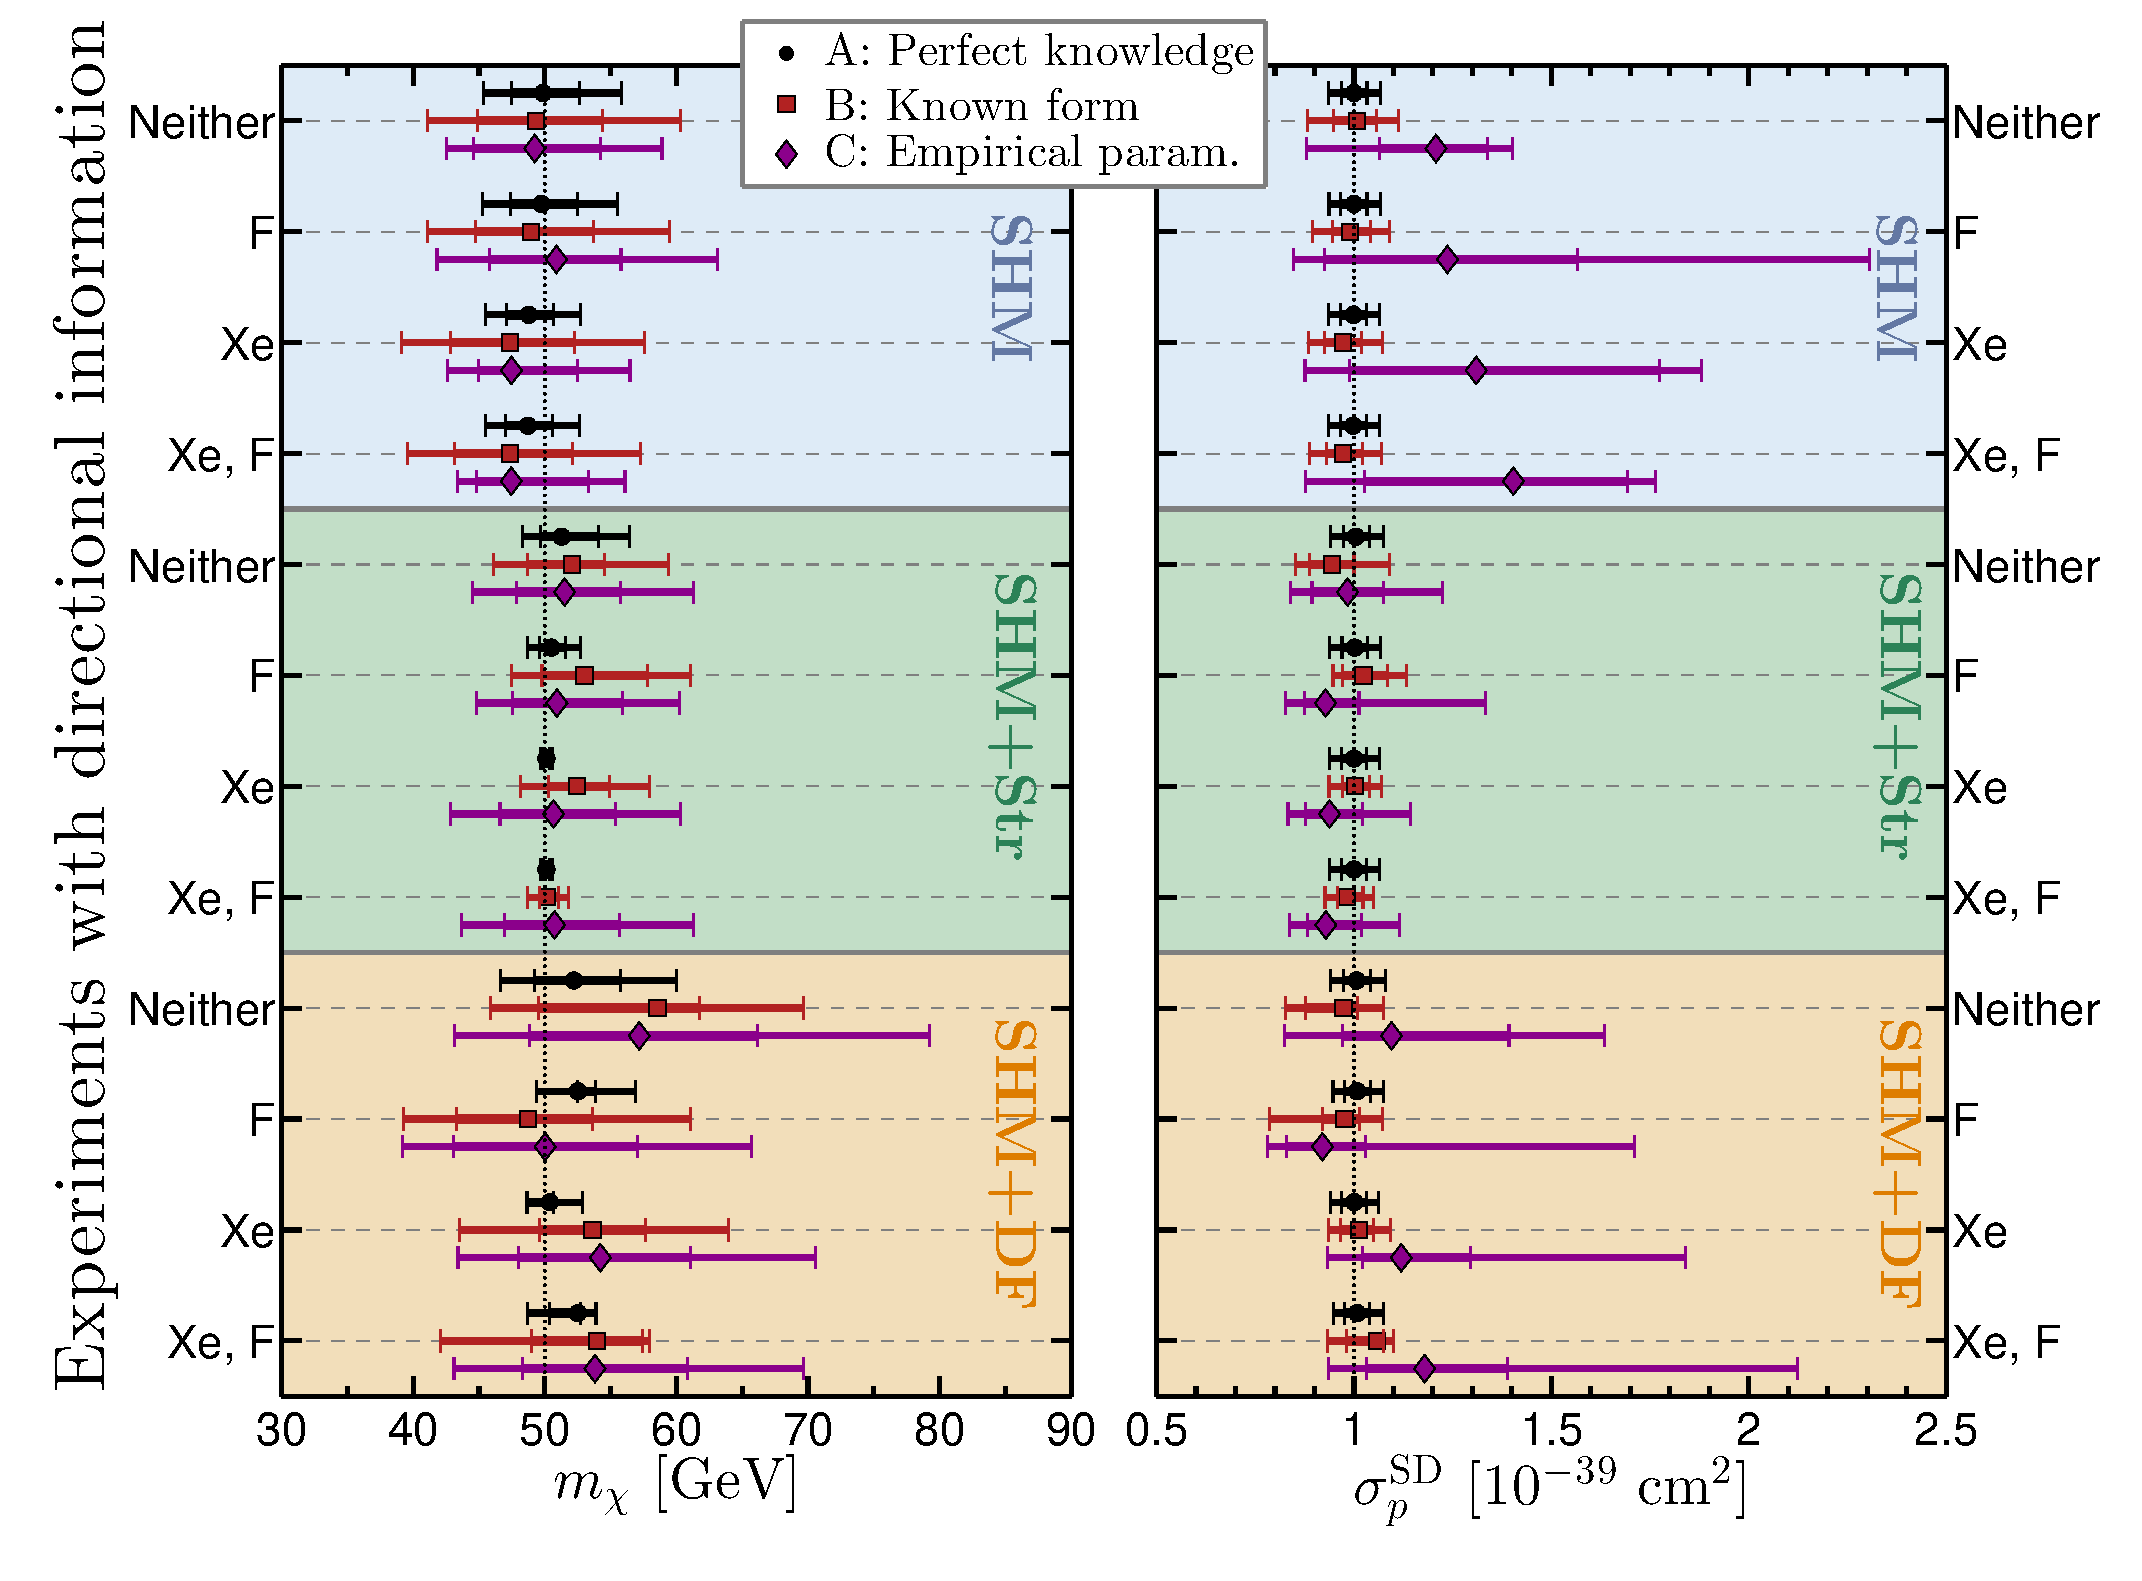
\includegraphics[width=0.95\textwidth]{Figures/mx-recon.eps}
\caption[Reconstructed confidence intervals for WIMP mass and cross section]{Reconstructed 68\% and 95\% confidence intervals for WIMP mass ({\bf left}) and SD cross section ({\bf right}) under each halo model (from top to bottom): the SHM (blue region), the SHM with stream (green) and SHM with debris flow (orange) models. The intervals are shown as a function of the amount of directional information included. The black points and error bars show the reconstruction using perfect knowledge of the DM distribution (Method A), red squares show reconstructions when the functional form is known (Method B), and purple diamonds when a general empirical form for the speed distribution is assumed (Method C). The input (i.e. correct) values are shown as vertical dotted lines.}\label{fig:mx-recon}
\end{figure}
In the right panel of Fig.~\ref{fig:mx-recon}, we show the corresponding limits on the WIMP-proton SD cross section. In this case, the contrast between Methods A \& B and Method C is more stark. Using the former two methods, reconstruction of $\sigma_p^\mathrm{SD}$ is relatively precise, with an uncertainty of less than 10\%. However, for Method C, the intervals are much wider, extending in most cases up to large values of the cross section. This results from a known degeneracy between the WIMP cross section and the shape of the speed distribution in halo-independent approaches~\cite{Kavanagh:2013wba}. An increase in the fraction of low-speed particles below the direct detection threshold has no effect on the event rate, provided the value of the cross section is increased to counteract the reduced fraction of high-speed particles.

For Method A and B we see that in most cases increasing the quantity of directional information (reading Fig.~\ref{fig:mx-recon} from top to bottom in each halo model) leads to better measurements of the WIMP mass. In contrast, the error on $\sigma_p^{\rm SD}$ found with Methods A and B is largely insensitive to the amount of directionality as the key information for reconstructing a cross section is the total number of events. For Method C, there is little increase in precision as the amount of directional information is increased; reconstruction of the WIMP mass in this case depends primarily on obtaining the correct distribution of recoil {\it energies} in each experiment. 

\subsection{Velocity distribution shape}\label{sec:directional_shape}
\begin{figure}
\centering     %%% not \center
\subfigure[{\bf SHM:} Directionality in F only.]{\label{fig:veldist-a}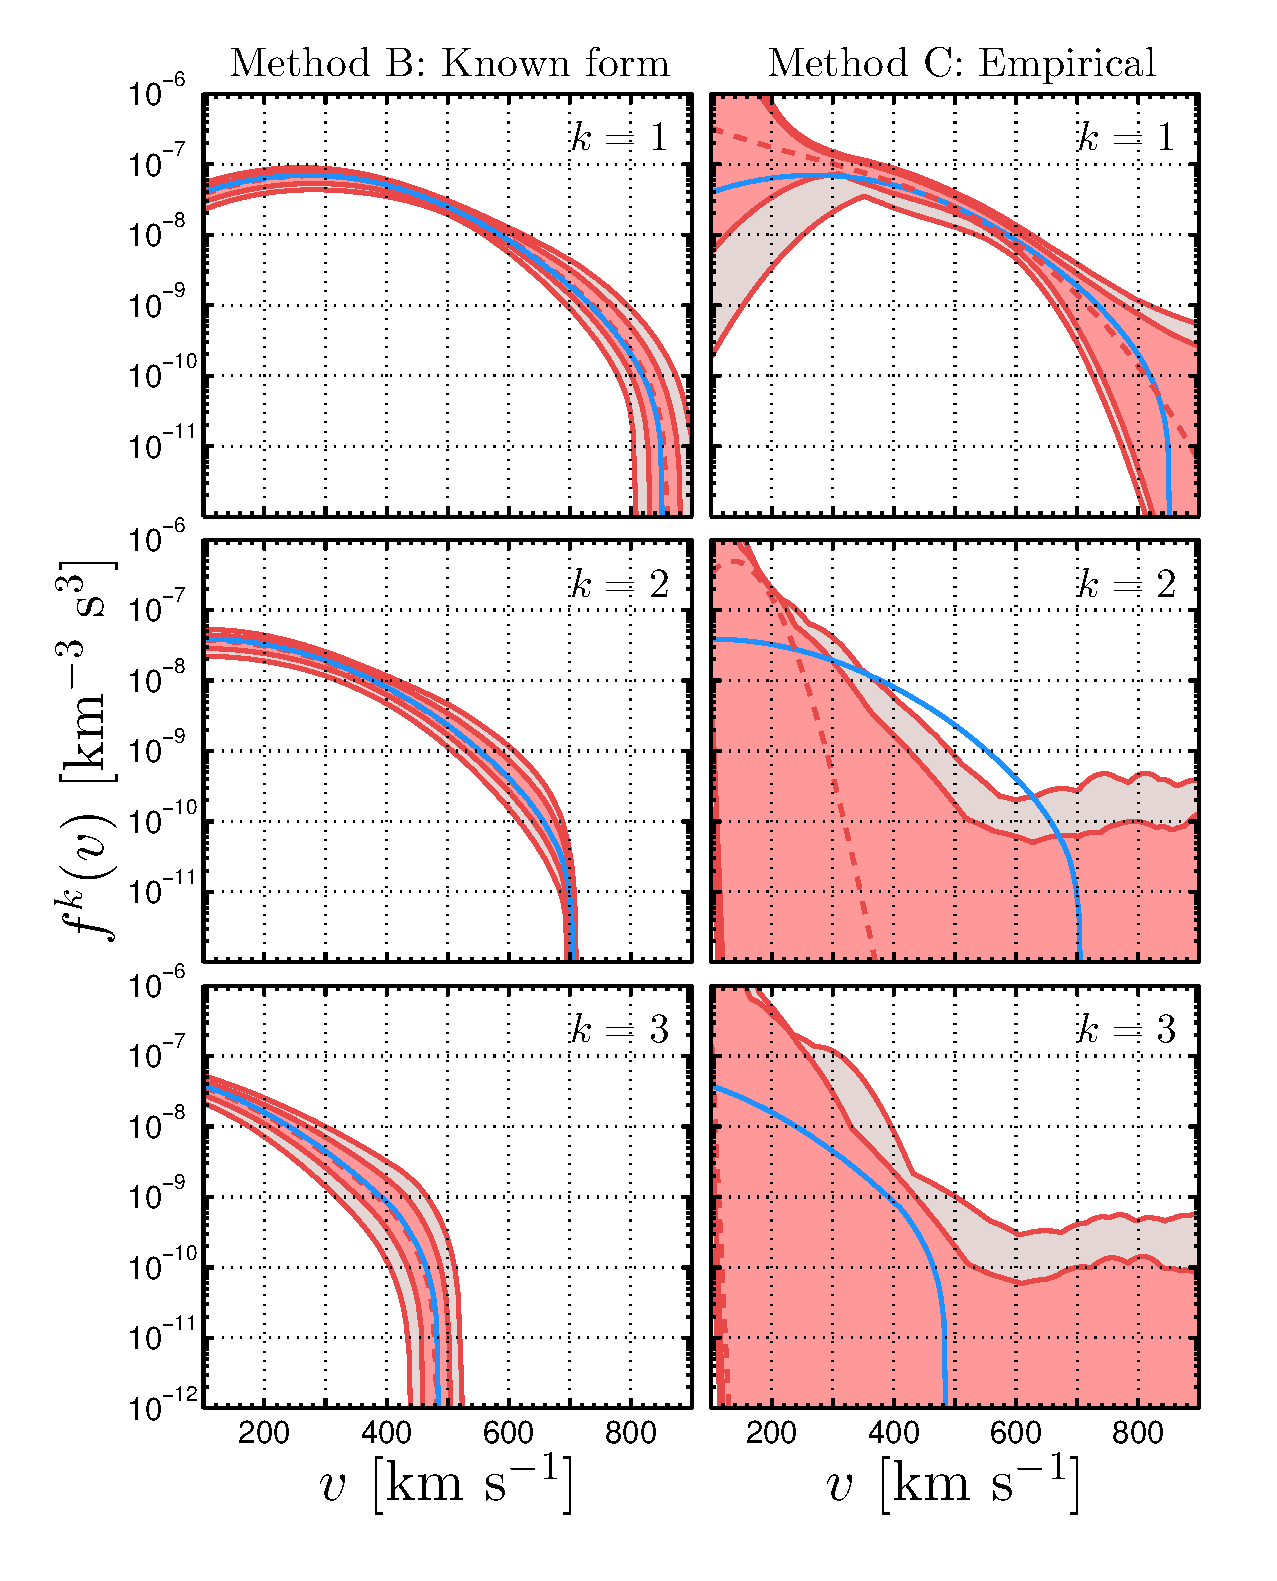
\includegraphics[width=0.49\textwidth]{Figures/veldist-SHM-Xe-N-F-D.eps}}
\subfigure[{\bf SHM:} Directionality in F and Xe.]{\label{fig:veldist-b}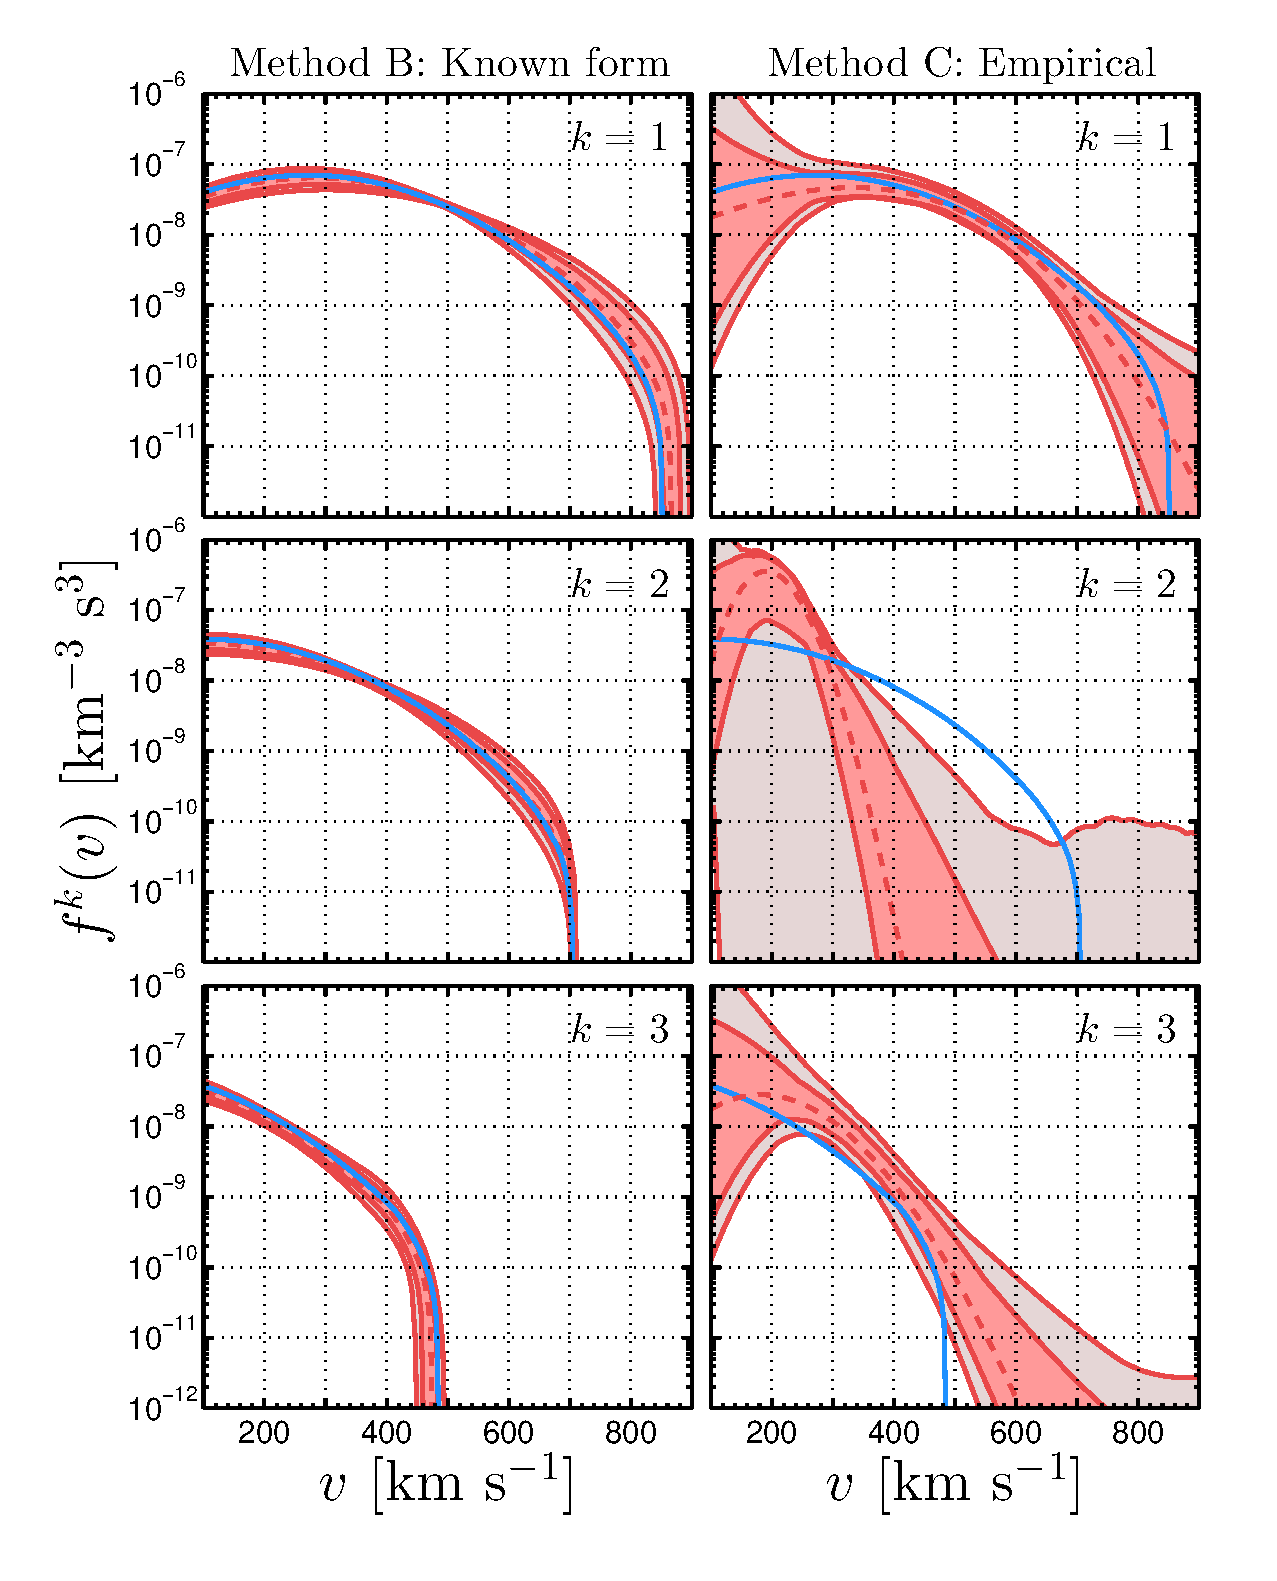
\includegraphics[width=0.49\textwidth]{Figures/veldist-SHM-Xe-D-F-D.eps}}

\subfigure[{\bf SHM+Str:} Directionality in F and Xe.]{\label{fig:veldist-c}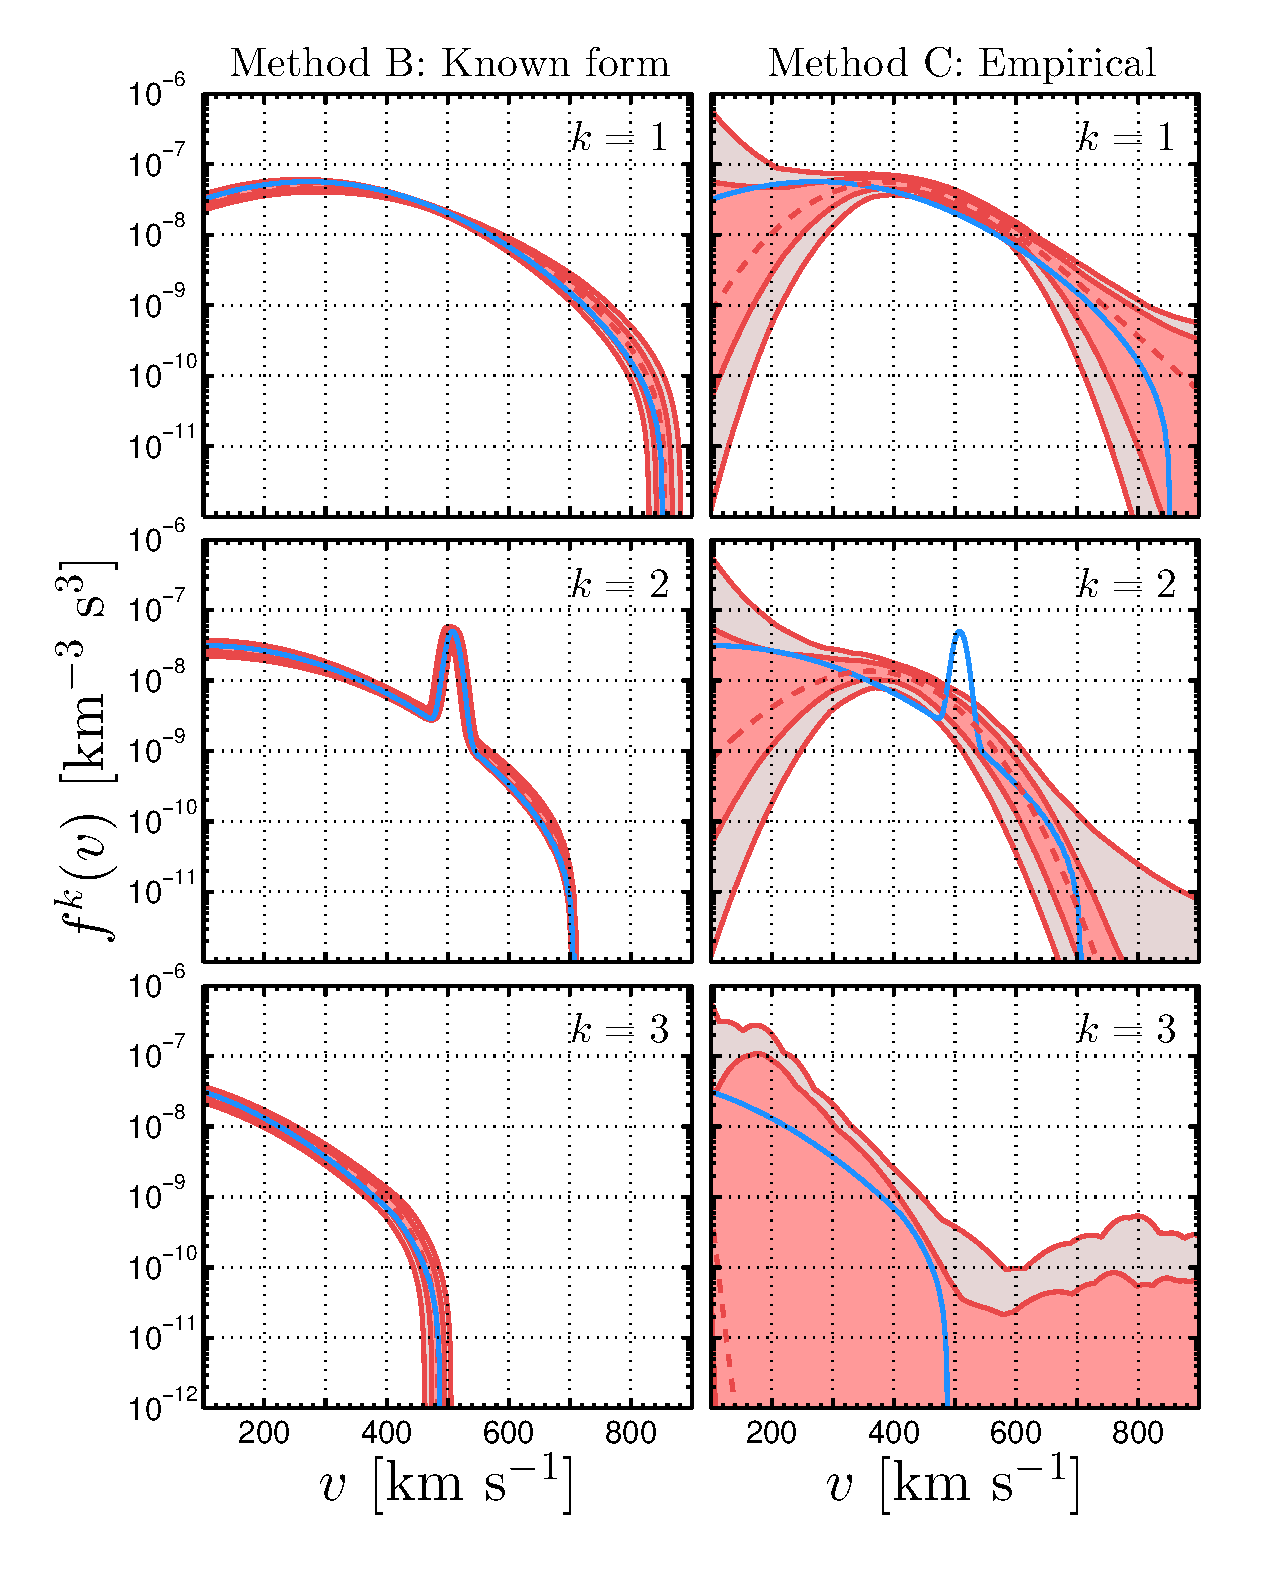
\includegraphics[width=0.49\textwidth]{Figures/veldist-STR-Xe-D-F-D.eps}}
\subfigure[{\bf SHM+DF:} Directionality in F and Xe.]{\label{fig:veldist-d}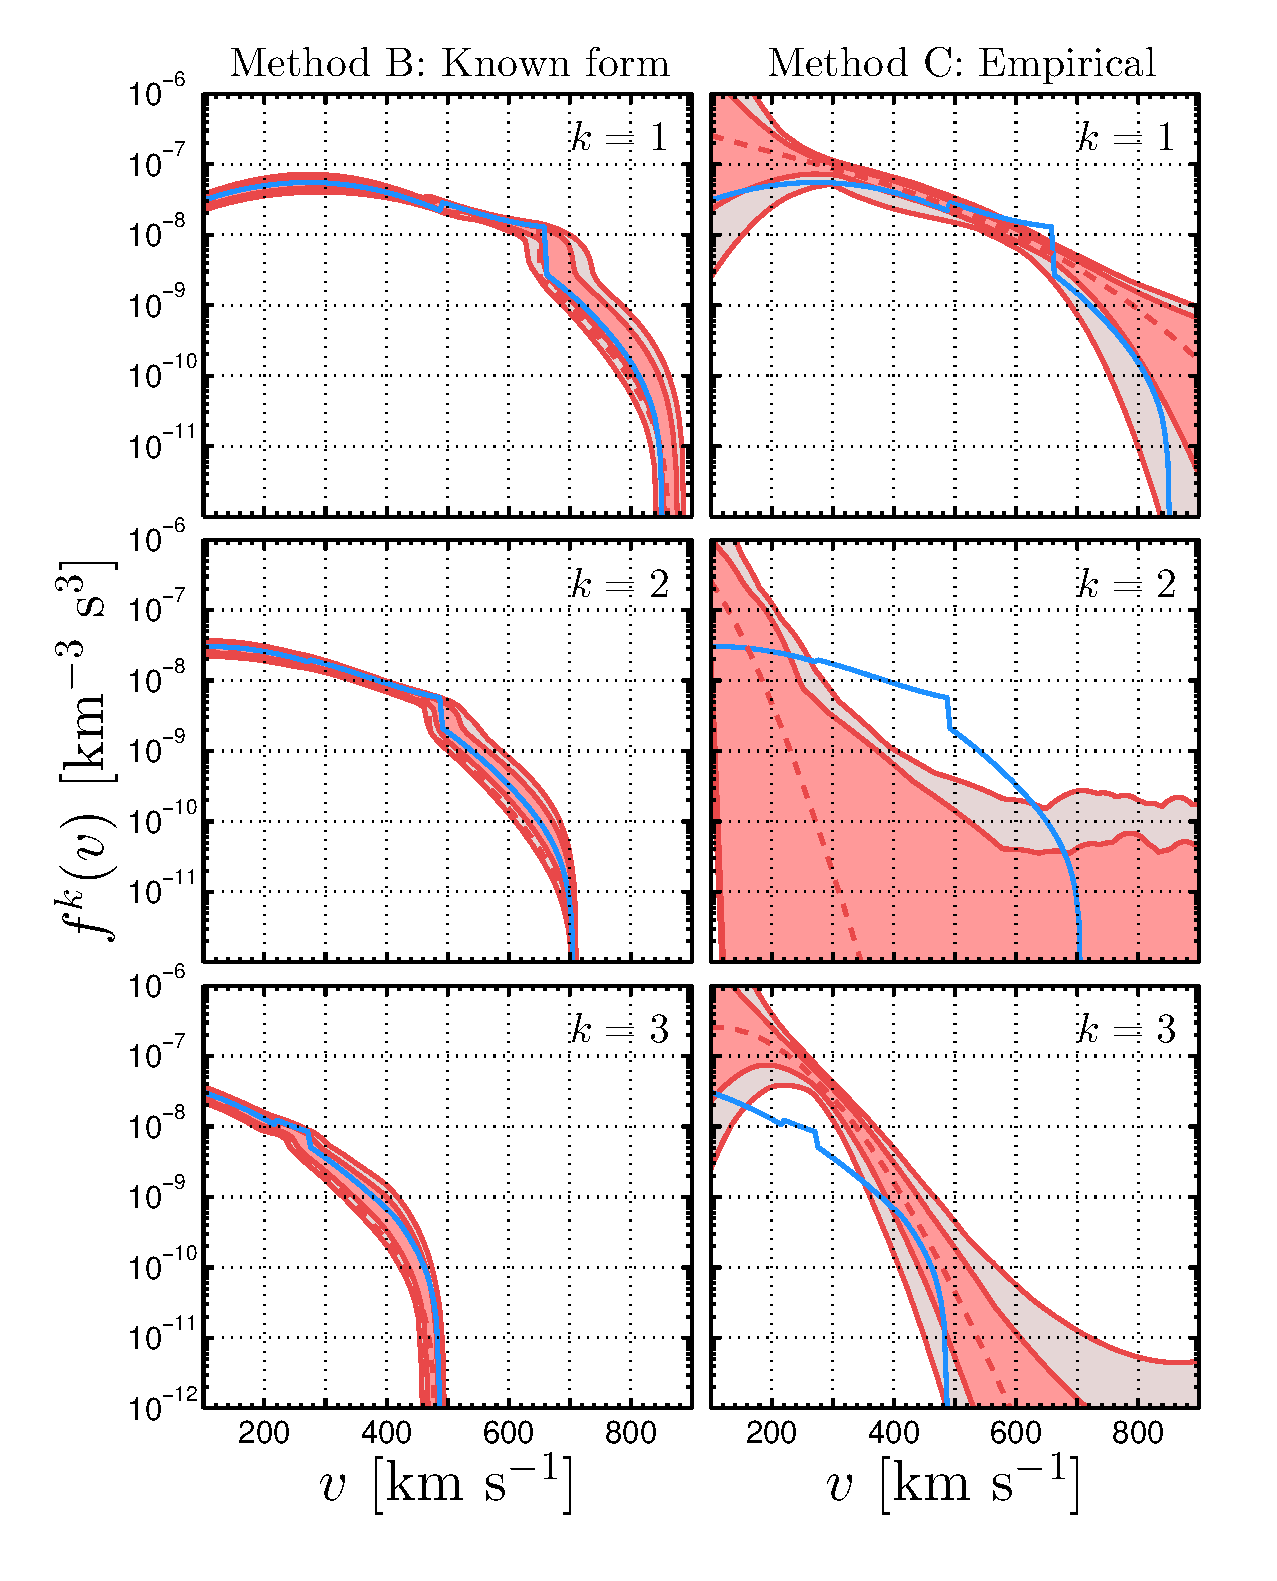
\includegraphics[width=0.49\textwidth]{Figures/veldist-DF-Xe-D-F-D.eps}}
\caption[Reconstructed binned velocity distributions]{Reconstructed velocity distribution averaged over each of the three angular bins ($k=1,2,3$) defined in Eq.~(\ref{eq:bins}). The left column in each subfigure shows the results for Method B (known functional form) while the right column shows results for Method C (empirical parameterisation). The correct underlying velocity distribution is shown with a solid blue line. The best fit reconstruction is shown as a red dashed line, while the 68\% and 95\% intervals are given by the inner and outer red shaded regions.}\label{fig:veldist}
\end{figure}

We now present results for the shape of the reconstructed velocity distribution in each of the three angular bins:
\begin{align}\label{eq:bins}
\begin{split}
{\rm `Forward\textrm{'}}\quad &k = 1: \qquad \theta \in \left[ 0, \pi/3\right]\,, \\
{\rm `Transverse\textrm{'}}\quad &k = 2: \qquad \theta \in \left[ \pi/3, 2\pi/3 \right]\,, \\
{\rm `Backward\textrm{'}}\quad &k = 3: \qquad \theta \in \left[ 2\pi/3, \pi\right]\,. \\
\end{split}
\end{align}
For the discretised velocity distribution of Method C, we simply construct the velocity distribution in the $k$th bin, $f^k(v)$, from the $\{a_m^{(k)}\}$ parameters according to Eq.~(\ref{eq:polynomialparam}). For Method B, we average the full velocity distribution (described by a given set of parameters) over each angular bin in $k$:
\begin{equation}\label{eq:fk}
f^{k}(v) = \frac{\int_{\cos(k\pi/N)}^{\cos((k-1)\pi/N)} f(\mathbf{v}) \, \mathrm{d}\cos\theta}{\cos((k-1)\pi/N) - \cos(k\pi/N)}\,.
\end{equation}
At each speed $v$, 68\% and 95\% confidence intervals are calculated from the distribution of values of $f^k(v)$ by profiling over the values at all other speeds (as well as the mass and cross section). Figure~\ref{fig:veldist} compares the reconstructed distributions $f^k(v)$ in the two Methods B and C (red curves) as well as `true' distributions obtained by applying Eq.~(\ref{eq:fk}) to the correct underlying distribution (solid blue curve). We describe each subfigure of Fig.~\ref{fig:veldist} in turn.

{\bf Figure~\ref{fig:veldist-a}} shows results for the SHM distribution with directional sensitivity in only the fluorine experiment. For Method B (left column), the best fit velocity distribution (dashed red) follows the underlying distribution closely. The strongest constraints are in the forward bin ($k=1$) in the range $v \sim 300~-~500 \kms$ where the distribution of recoils is most focused. Using Method C (right column), we also obtain a good fit to the velocity distribution in the forward bin. At high and low speeds, the confidence intervals widen as the recoil rate is insensitive to the shape of the speed distribution outside of the energy window $[E_\mathrm{th}, E_\mathrm{max}]$. In the transverse and backward bins, where very few of the fluorine events lie, the velocity distribution is also poorly constrained.

{\bf Figure~\ref{fig:veldist-b}} we now have both xenon and fluorine detectors with directional sensitivity. Comparing with the previous case, we see that the constraints are tightened. For Method B, this is perhaps most pronounced for the $k = 3$ bin due to the lower threshold of the xenon detector producing a distribution of nuclear recoils which is less strongly peaked in the forward direction. This means that more recoils are observed in the backward and transverse bins, improving the overall reconstruction. Similarly, constraints in the $k=3$ bin for Method C are also now stronger. However we note that the discretised velocity distribution in the $k=2$ bin is significantly lower than the true distribution. This is because $f(\mathbf{v})$ is in fact a strong function of angle across this bin. If we fixed $f^2(v)$ equal to the average of the true distribution across the entire bin, this would lead to an excess of recoils in the backwards direction and a deficit of recoils in the forward direction. Instead, the best fit form of $f^2(v)$ peaks at low speeds, with only a small contribution above the experimental thresholds. There is then still sufficient freedom in $f^1(v)$ and $f^3(v)$ to fit the observed distribution of recoils. 

{\bf Figure~\ref{fig:veldist-c}} shows results for the SHM+Str model when both experiments are directionally sensitive. As before, with Method B the velocity distribution is well reconstructed, and in fact achieves a slightly better reconstruction than under the SHM model due to the greater freedom in the larger parameter space. For Method C however the 4-parameter polynomial fit in each angular bin is not sufficient to pick out a feature as sharp as a stream. Nonetheless, the reconstruction does point towards an excess of particles in the $k=2$ bin in a wide range around the stream speed of $400 \kms$. To compensate, the best fit form of $f^3(v)$ is suppressed.

{\bf Figure~\ref{fig:veldist-d}} we show finally, the reconstructed SHM+DF model. For Method B, the confidence intervals are wider than before. This is because the debris flow is a much broader feature in the velocity distribution and therefore has a stronger degeneracy with the parameters of the SHM. For Method C, we see a slightly flatter reconstructed distribution in the $k=1$ bin than for previous benchmarks, as well as narrower uncertainty bands up to around $550 \kms$ caused by the enhancement in high energy recoils in the forward direction.

In this section, we have observed that a discretised parameterisation can approximate the shape of the bin-averaged velocity distribution when large numbers of events are observed in a particular direction. In other cases, there appears to be a discrepancy between the reconstructions and the underlying distribution. However, this is only a problem if we interpret the $f^k(v)$ distributions that are reconstructed as representing the average of the true speed distribution across the $k$th bin. This is a slightly unfair comparison as we should interpret the $f^k(v)$ functions as empirical fits to the full velocity distribution. As shown in the SHM+Str case, this comparison can be used to look for clear features in the distribution, but it is difficult to make statistically concrete statements about the underlying velocity distribution from the shapes of $f^k(v)$. In light of this, we now discuss some simple measures which can be used to extract information and compare different models in a more useful way.

\subsection{Velocity parameters}\label{sec:directional_parameters}
We now wish to find a model independent and simple way of discriminating between our three halo models. We can do this by mapping the reconstructions as presented in the previous section onto a set of physical parameters that can be extracted by both methods (B and C). We calculate mean values for the velocity parallel and transverse to the lab motion, $\langle v_y\rangle$ and $\langle v_T^2 \rangle$ respectively:
\begin{equation}\label{eq:vy}
\langle v_y \rangle = \int \mathrm{d}v \,\int_{0}^{2\pi} \mathrm{d}\phi \, \int_{-1}^1 \mathrm{d}\cos\theta \, (v\cos\theta)\, v^2 f(\mathbf{v}) \, ,
\end{equation}
and
\begin{equation}\label{eq:vT}
\langle v_T^2 \rangle = \int \mathrm{d}v \,\int_{0}^{2\pi} \mathrm{d}\phi \, \int_{-1}^1 \mathrm{d}\cos\theta \, (v^2(1-\cos^2\theta))\, v^2 f(\mathbf{v}) \, .
\end{equation}

\begin{figure}
\centering
	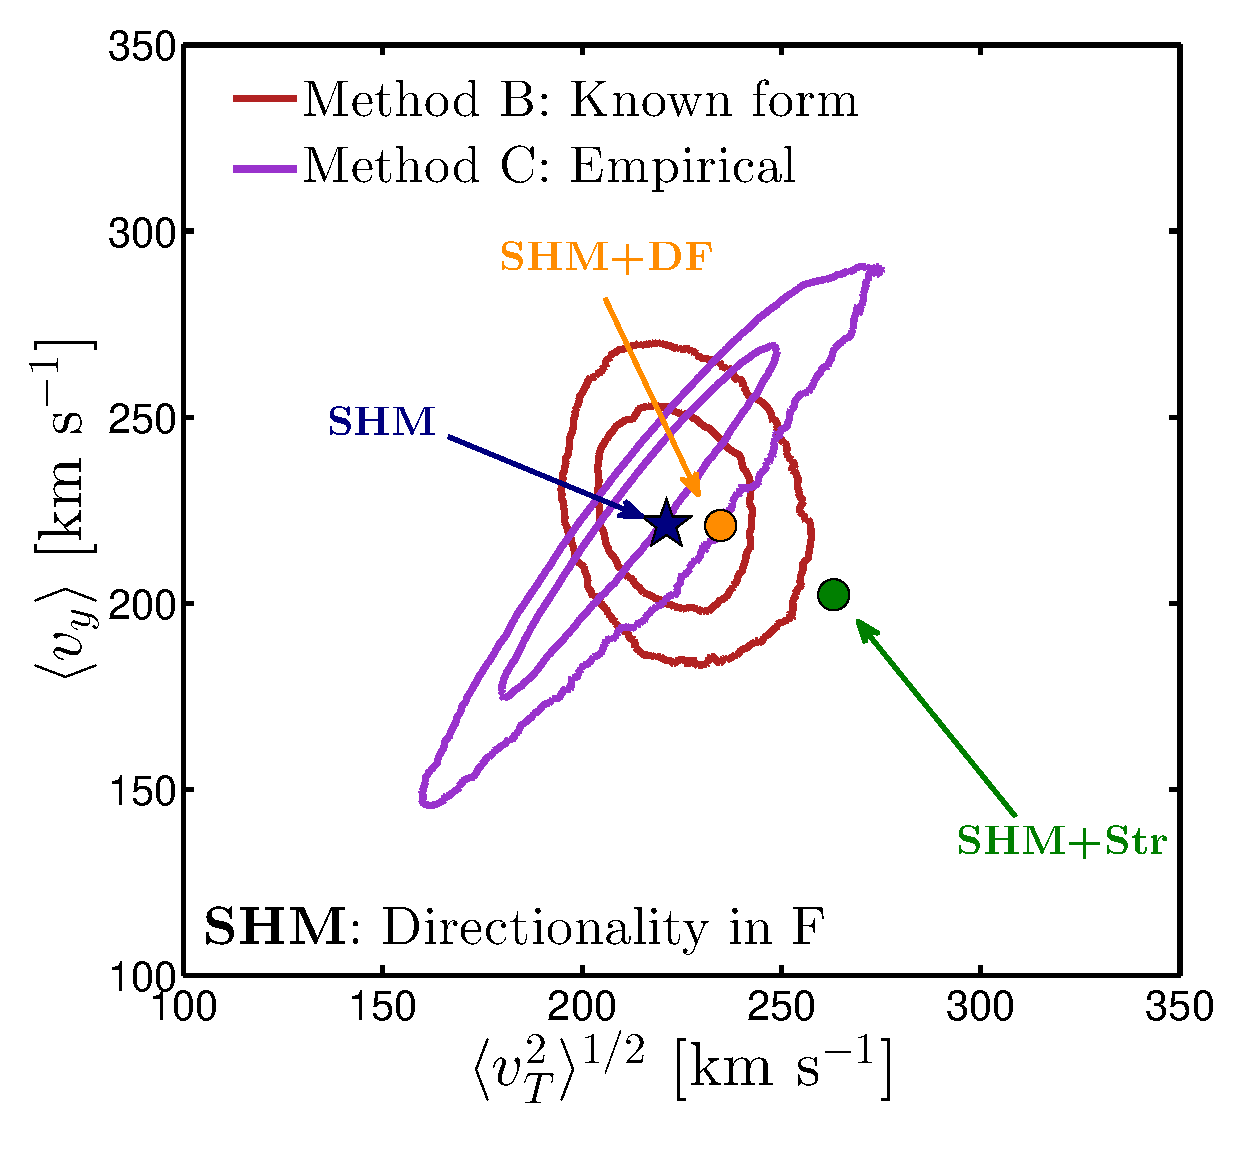
\includegraphics[width=0.32\textwidth]{Figures/vyvT-SHM-Xe-N-F-D.eps}
	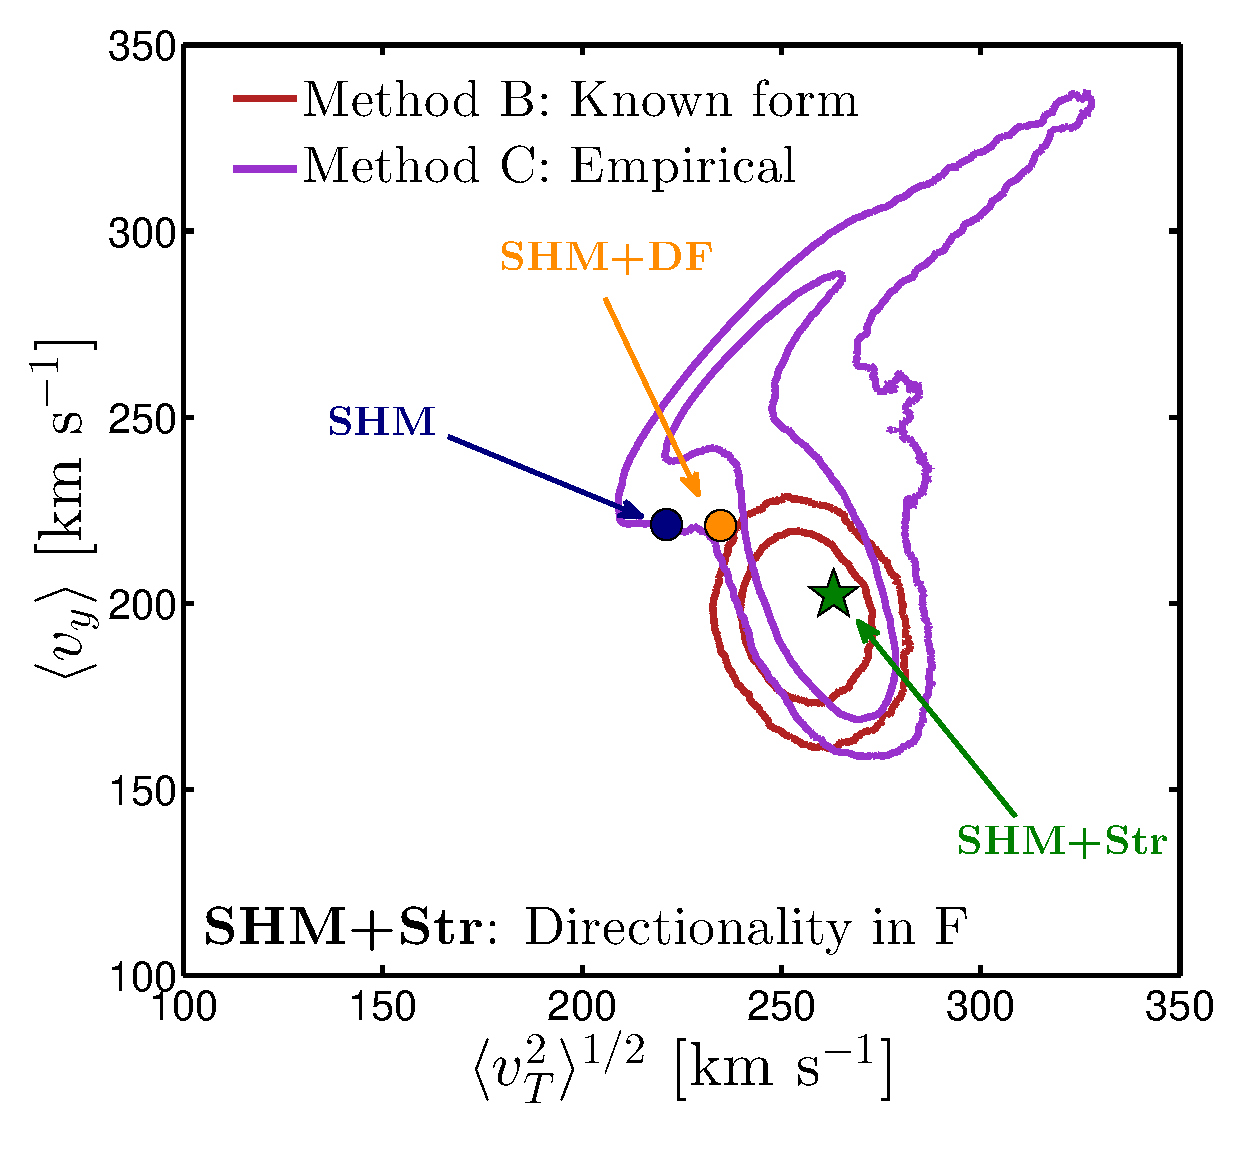
\includegraphics[width=0.32\textwidth]{Figures/vyvT-STR-Xe-N-F-D.eps}
	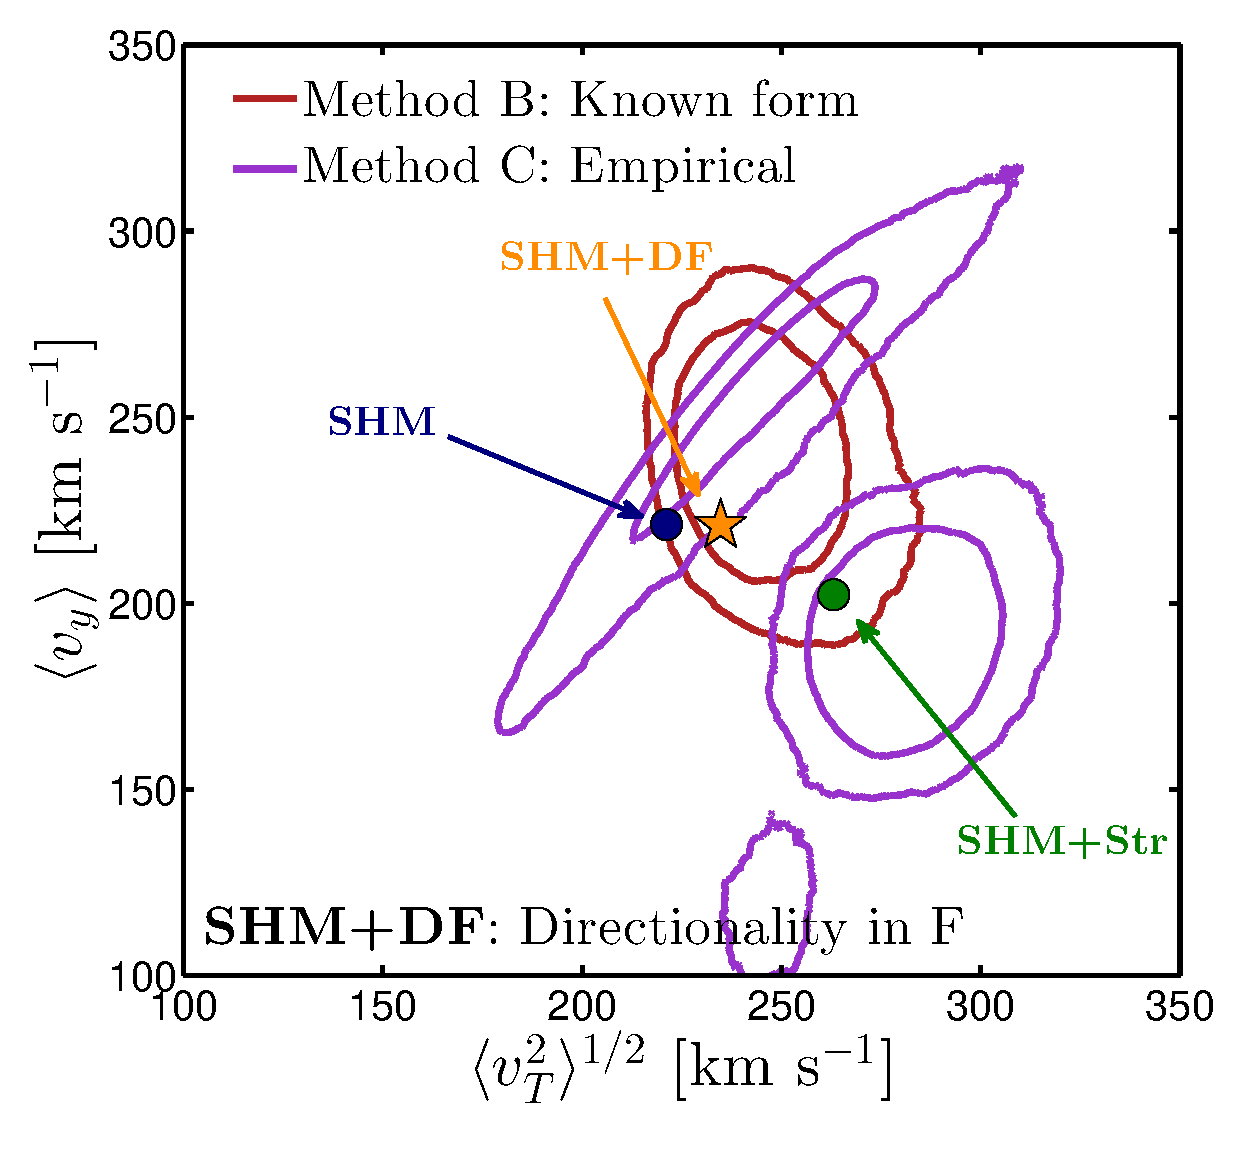
\includegraphics[width=0.32\textwidth]{Figures/vyvT-DF-Xe-N-F-D.eps}
	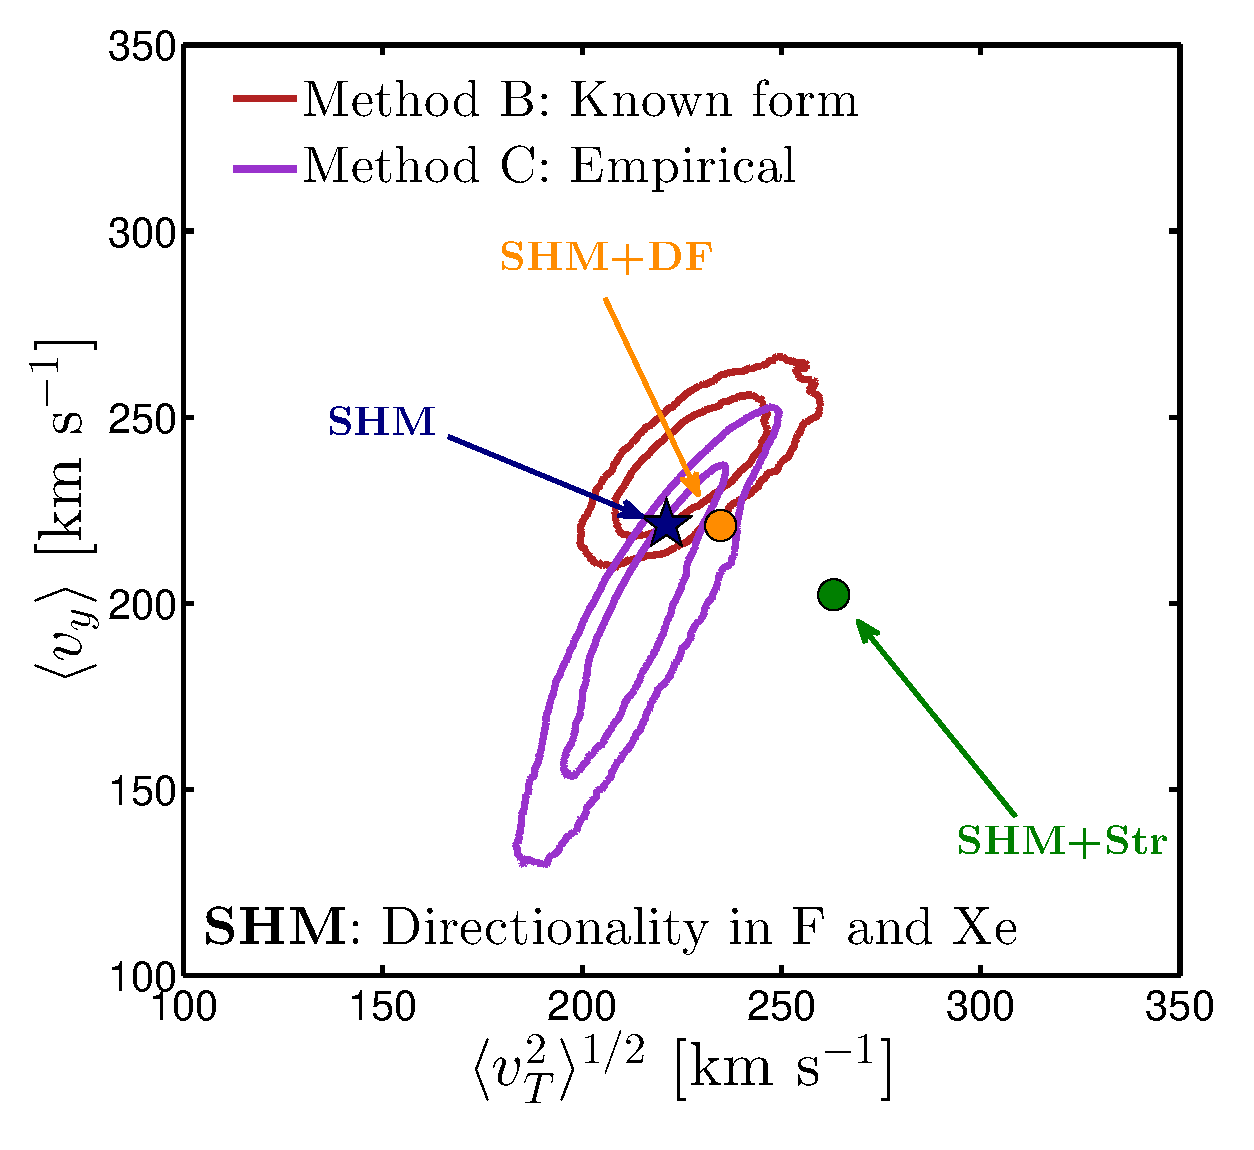
\includegraphics[width=0.32\textwidth]{Figures/vyvT-SHM-Xe-D-F-D.eps}
	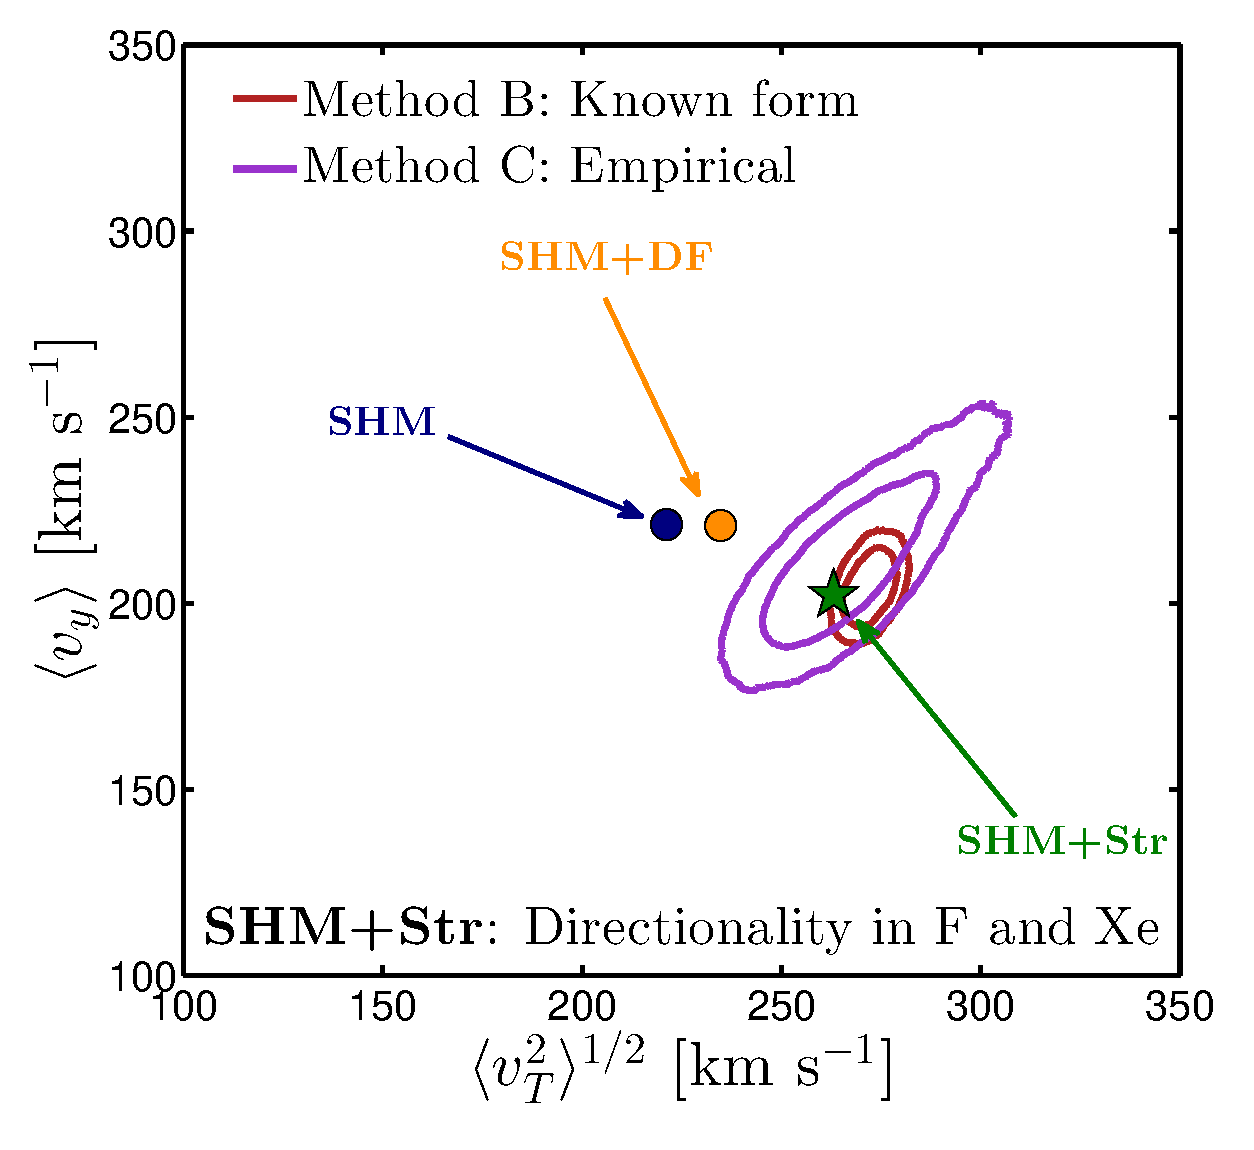
\includegraphics[width=0.32\textwidth]{Figures/vyvT-STR-Xe-D-F-D.eps}
	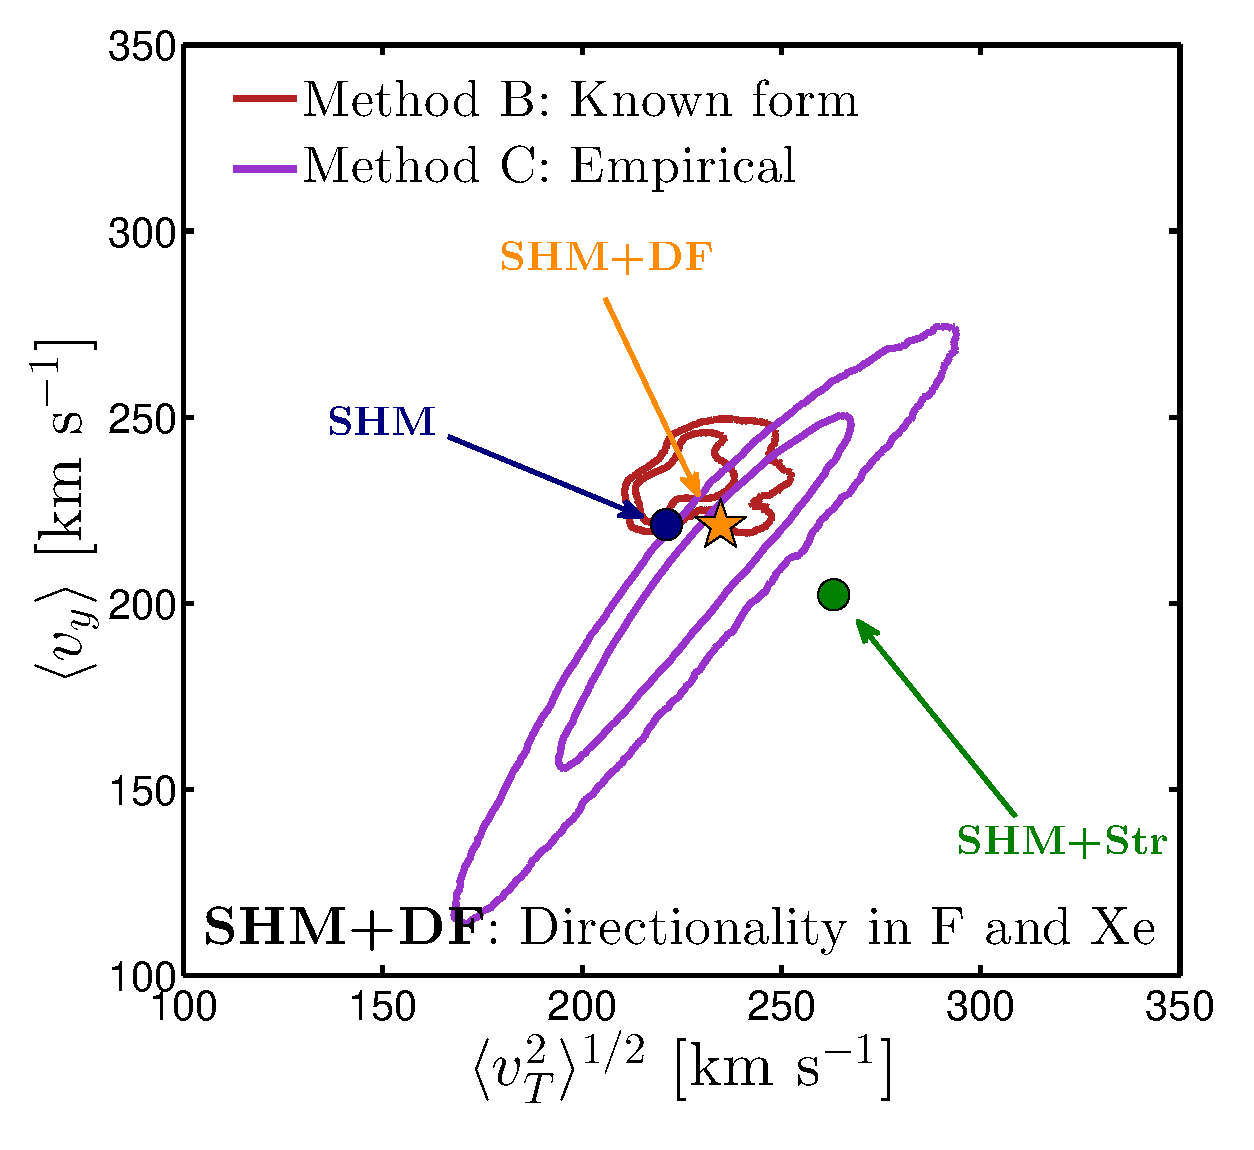
\includegraphics[width=0.32\textwidth]{Figures/vyvT-DF-Xe-D-F-D.eps}
    \caption[Reconstructed parallel and transverse velocities for each halo model]{Mean values for the DM velocity parallel and transverse to the lab velocity, $\langle v_y \rangle$, and $\langle v_T^2 \rangle^{1/2}$. The 68\% and 95\% confidence intervals obtained using reconstruction methods B and C are shown as pairs of red and purple contours respectively. We show results for all three halo models (SHM, SHM+Str and SHM+DF in each column from left to right) and for directionality in a single experiment (top row) and in both experiments (bottom). The correct values of $\langle v_y \rangle$ and $\langle v_T^2 \rangle^{1/2}$ for each halo model are shown as labelled markers (the input model is indicated with a star in each case).}\label{fig:vyvT}
\end{figure}
In Fig.~\ref{fig:vyvT} we show the reconstructed velocity distribution in each halo model mapped onto the $\langle v_y \rangle$-$\sqrt{\langle v_T^2 \rangle}$ plane. Here again we make the comparison between only fluorine having directional sensitivity (top row) and both experiments being directionally sensitive (bottom). For Method B, the values of the physical parameters ($v_0$, $\sigma_v$, $v_{\rm str}$, etc.) are typically well constrained, meaning that $\vy$ and $\vT$ are also well constrained, with roughly Gaussian error contours.  In contrast, the reconstructions using Method C exhibit a pronounced degeneracy along the direction of $\vy \propto \vT$ for many of the benchmarks. This is due to the fact that the $k=1$ and $k=3$ bins contribute to the mean values of both the forward \textit{and} transverse DM speeds. For example, increasing $f^1(v)$ leads to an increase in $\vy$ but also a proportional increase in $\vT$, because the particles are assumed to be distributed equally in $\theta$ across the bin. The position of the contours in $\vT$ is typically dominated by the $k=2$ bin, which contributes to $\vT$ and not to $\vy$. 

For both reconstruction methods and for directionality in either one or both experiments, the underlying benchmark values of $\vy$ and $\vT$ always lie within the 95\% confidence regions. The SHM and SHM+DF models are hardest to distinguish. The debris flow is isotropic in the Galactic frame, so the net velocity of the DM particles in the lab frame is due entirely to $\textbf{v}_\textrm{lab}$. Thus, we have $\vy \sim v_0$ as in the SHM. The debris flow is a rather broad feature leading only to a mild increase in $\vT$. Indeed, with the SHM benchmark dataset, the SHM+DF model cannot be rejected at the 95\% confidence level using either reconstruction method.  

The SHM+Str is much more easily distinguished from the other two benchmarks. The stream velocity is almost perpendicular to the Earth's velocity, leading to a decrease in $\vy$ and a marked increase in $\vT$. For the SHM mock dataset (left column), the SHM+Str is clearly excluded with both Methods, even when only the fluorine detector has directionality. Under the SHM+Str dataset the addition of the stream leads to a mild increase in the number of fluorine events in the transverse recoil direction, while still producing no events in the backward direction. This data can be well fit by adding a substantial population of particles in the $k=2$ bin (causing the lower round part of the contours in the upper middle panel of Fig.~\ref{fig:vyvT}) or alternatively by enhancing the forward $k=1$ population at low speeds (causing the upper straight part of the contours). Including xenon directionality (lower middle panel of Fig.~\ref{fig:vyvT}), adds roughly equal numbers of forward and transverse recoils, breaking the degeneracy and allowing the SHM+Str model to be unequivocally distinguished from the other benchmarks.

Using the SHM+DF dataset  with directionality in fluorine only (upper right panel of Fig.~\ref{fig:vyvT}), we notice there are three distinct regions fit by Method C. The three regions correspond to enhanced populations of DM particles in each bin. The Debris Flow contributes in all 3 angular bins and will typically produce higher energy recoils than the SHM alone (as $v_f > v_0$). An increased high-speed population in any of the velocity bins will then improve the fit to the data. Once again, adding xenon directions breaks the degeneracy between the three regions and in this case the SHM+Str benchmark can be rejected.

These results indicate that mapping the reconstructed velocity distributions onto the parameters $\vy$ and $\vT$ can be a reliable and unbiased way of trying to distinguish different underlying halo models. The SHM and SHM+DF models are typically difficult to distinguish, while the SHM+Str has sufficiently different properties (a large transverse velocity) that it can be clearly excluded in many cases.

\subsection{Folded reconstructions}
As discussed in Sec.~\ref{sec:directional_expts}, a major concern for current directional detection experiments is the ability to measure the forward or backward going sense of a reconstructed recoil track. We define the `folded' recoil spectrum that would be observed in experiments without any head-tail effect as,
\begin{equation}
 \frac{\mathrm{d}^2R_\mathrm{fold}}{\mathrm{d}E_r\mathrm{d}\Omega_r} = \frac{\mathrm{d}^2R}{\mathrm{d}E_r\mathrm{d}\Omega_r}\bigg|_{-\qhat}+\frac{\mathrm{d}^2R}{\mathrm{d}E_r\mathrm{d}\Omega_r}\bigg|_{+\qhat} \, .
\end{equation}
Following the results of Sec.~\ref{sec:directional_parameters} we show again the expectation values for the parallel and transverse velocities with respect to the direction of the Earth's motion. In this case for brevity we include only the result for the case in which both fluorine and xenon experiments have directional sensitivity, only now we remove their ability to tell the forward or backward going sense of their nuclear recoils. The results are shown for each halo model in Fig.~\ref{fig:vyvT-folded}.

\label{sec:folded}
\begin{figure*}[t]
	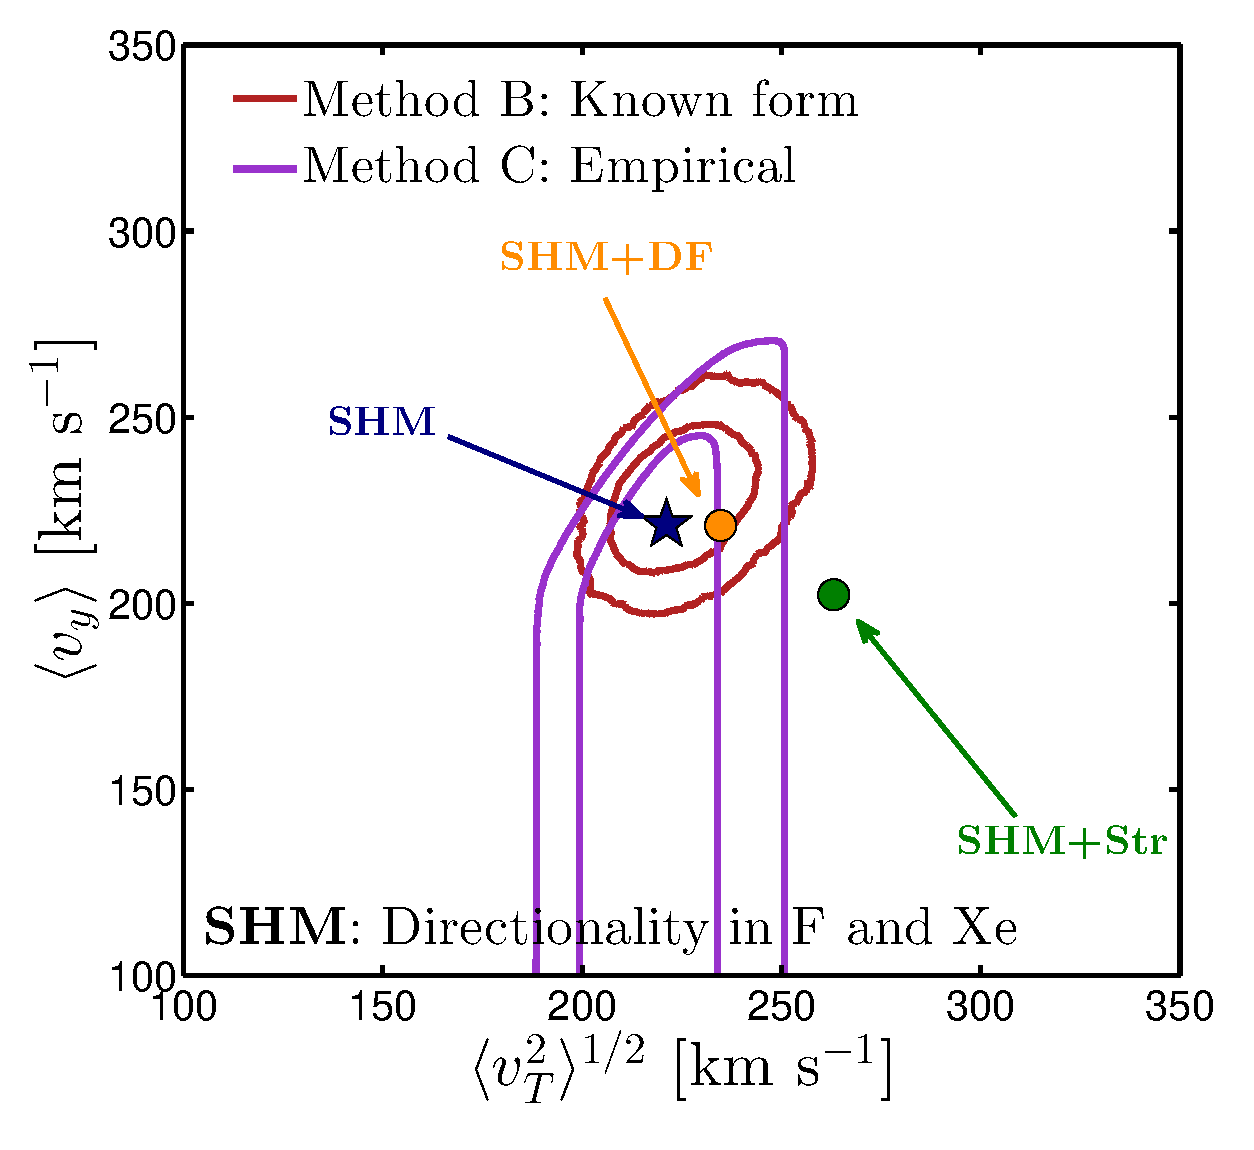
\includegraphics[width=0.32\textwidth]{Figures/vyvT-SHM-Xe-D-F-D-folded.eps}
	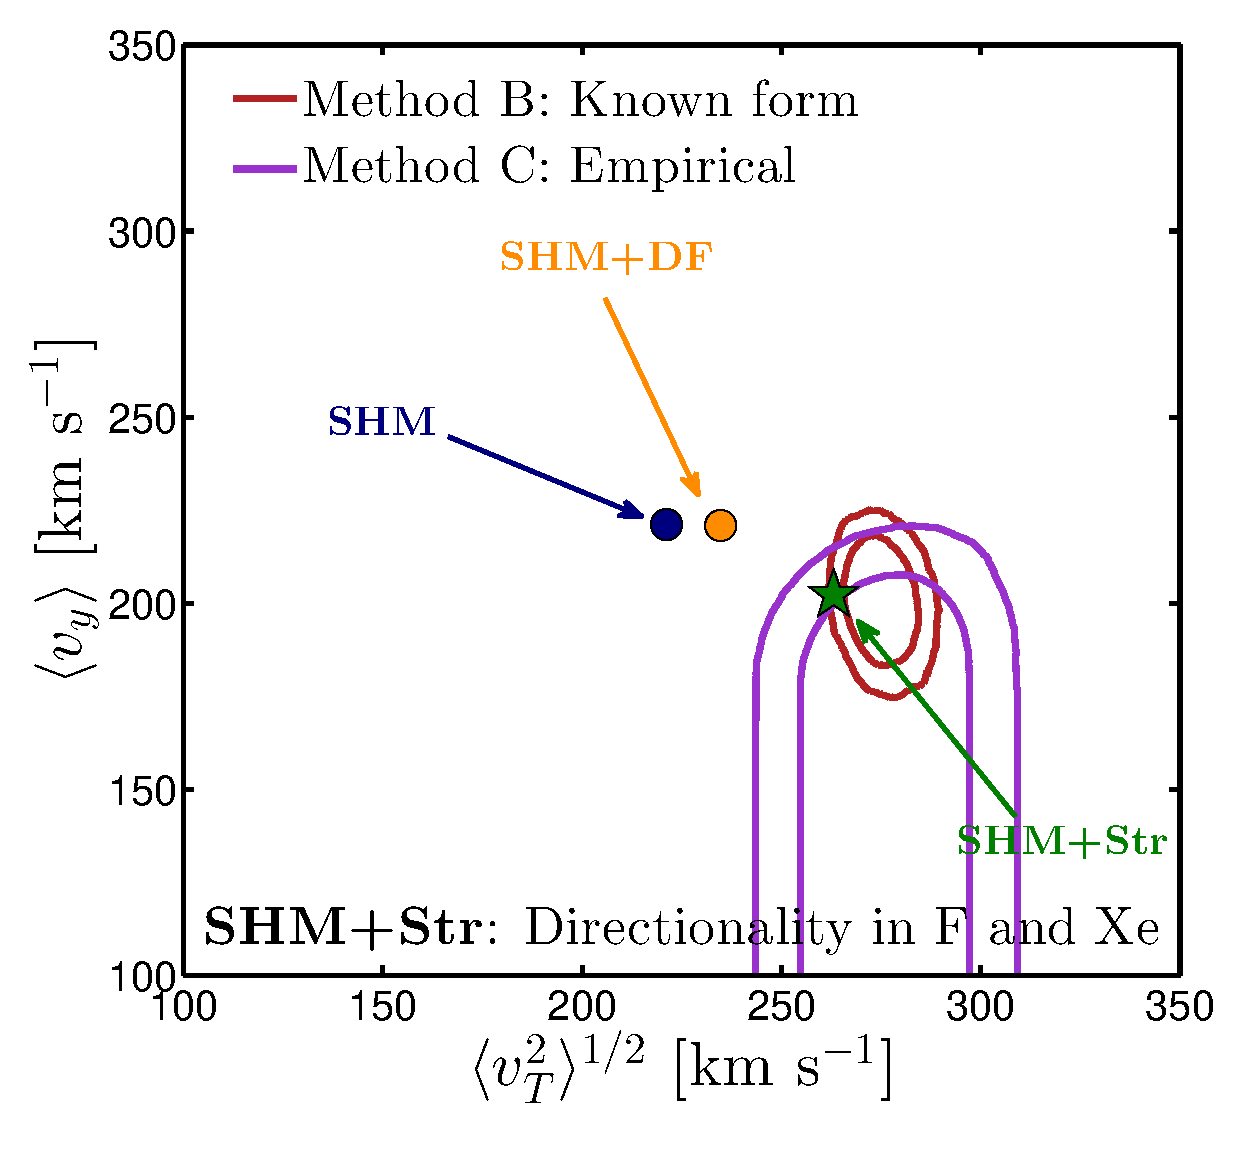
\includegraphics[width=0.32\textwidth]{Figures/vyvT-STR-Xe-D-F-D-folded.eps}
	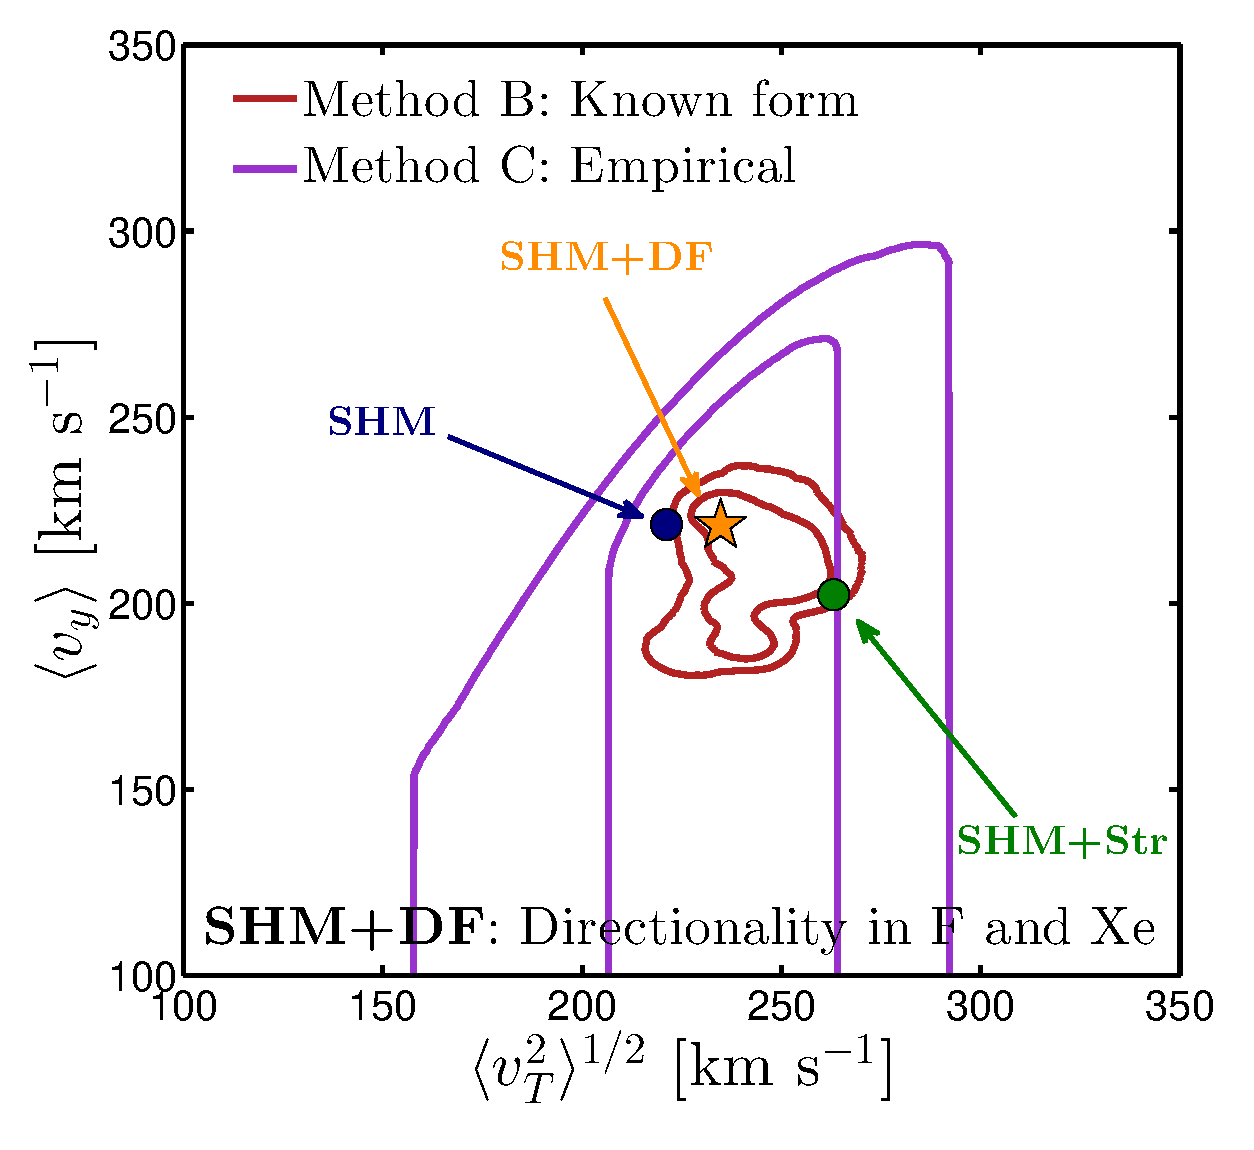
\includegraphics[width=0.32\textwidth]{Figures/vyvT-DF-Xe-D-F-D-folded.eps}
    \caption[Reconstructed parallel and transverse velocities with folded data]{Mean values for the DM velocity parallel and transverse to the lab velocity, $\langle v_y \rangle$, and $\langle v_T^2 \rangle^{1/2}$, reconstructed when both experiments have directional sensitivity but lack sense recognition. The 68\% and 95\% confidence intervals obtained using reconstruction methods B and C are shown as pairs of red and purple contours respectively. We show the results for each halo model (from left to right), the SHM, the SHM+Str and SHM+Debris flow models. For Method C (purple), the contours extend all the way down to negative values of $\vy$, but for clarity we show only the region of parameter space near the benchmark values.}\label{fig:vyvT-folded}
\end{figure*}
With the removal of sense recognition the pronounced dipole feature of the angular distribution of recoils is reduced. Hence our directional experiments can no longer extract information about the asymmetry between forward and backward going recoils. For Method B there is only a small increase in the size of the contours for the SHM and SHM+Str models as in these cases there are large populations of recoils transverse to the folding so there is not a large reduction in sensitivity to the parameters that are being reconstructed. Whilst there is a larger uncertainty in the full 3-dimensional stream velocity in Method B, this uncertainty is disguised by the mapping onto $\vy$ and $\vT$ and the SHM and SHM+Str benchmarks can still be distinguished. However in the case of the SHM+DF model there is a moderate increase in the size of the contours in $\vy-\vT$. This is because some of the information regarding the velocity of the debris flow is encoded in the forward-backward asymmetry of the recoils.

For Method C, however, we see a complete degeneracy appearing in the results for all three halo models between positive and negative values of $v_y$ (although for clarity we display only positive values of $v_y$ here). This is to be expected as the folded distribution measured by Method C has no distinction between $\vy$ running parallel or anti-parallel to the Earth's motion. However as we have not removed as much transverse information, the shape of the contours in the $\vT$ direction remain relatively unchanged for the SHM and SHM+Str models. In particular, for data under the SHM+Str benchmark, the SHM and SHM+DF benchmarks can still be rejected at the 95\% confidence level. However, this is not the case for the SHM+DF model; the debris flow component has populations in both transverse and parallel directions so there is a major increase in the size of the contours in both $\vy$ and $\vT$. In this case all three benchmarks lie within the 68\% region.

\subsection{Summary}
In this Chapter we have explored a number of methods for reconstructing the velocity distribution from future directional experiments. We have focused in particular on using a general, empirical parameterisation to fit the velocity distribution and compared this with the case where the underlying form of the velocity distribution is known. This allows us to understand whether the two methods lead to different reconstructed parameter values (which may be indicative of biased reconstructions) and how much the constraining power of the experiments changes as we open up the parameter space with a more general fit.

Previous works have demonstrated that the WIMP mass can be recovered from non-directional direct detection experiments without making assumptions about the form of the speed distribution \cite{Peter:2011eu,Kavanagh:2013wba}. As we show in Fig.~\ref{fig:mx-recon}, such astrophysics-independent approaches can be successfully extended to directional experiments. In particular, the use of an approximate, discretised velocity distribution does not spoil the accurate reconstruction of the WIMP mass. Our empirical parameterisation typically leads to larger uncertainties than when the underlying form of the distribution is known, but we see no evidence of bias.

For reconstructing the velocity distribution, as demonstrated in Sec.~\ref{sec:directional_shape}, looking at the binned form may allow us to pick out key features but it is generally difficult to make comparisons or draw meaningful conclusions. Instead, we construct confidence intervals for the velocity averages $\vy$ and $\vT$. These measures of the shape of the distribution allow us to distinguish robustly between different underlying halo models. We find that with directionality only in a fluorine experiment, it may be possible to detect or reject the presence of a substantial stream with 95\% confidence. This is an improvement upon the results of Sec.~\ref{sec:directional_streams} as in this case we have assumed no knowledge about the underlying distribution and relies on fewer directional events. However, more isotropic features such as a debris flow are more difficult to distinguish from the SHM. Adding directionality in a xenon experiment allows us to break degeneracies in the shape of the velocity distribution and leads to good discrimination between models with and without a stream. The SHM and SHM+DF models remain harder to distinguish using this method, whether the underlying functional form is known or not.

In experiments without the ability to determine the sense of the nuclear recoils we see that the discretised approach suffers. This is because the $N=3$ binning is effectively reduced to 2 as the forward and backward bins are folded. The result of this is that it becomes impossible to precisely measure the average speed in the direction of the folding due to a degeneracy between positive and negative values. This is in line with the results of previous studies~\cite{Green:2007at,Billard:2014ewa} finding that the lack of sense recognition greatly reduces the power of directional experiments.

The benchmark examples we have chosen in this work enable us to broadly compare the success of a discretised parameterisation of the velocity distribution under a range of scenarios. However the parameter space that describes different classes of substructure, for instance streams, is large. It is unlikely that the conclusions drawn from our benchmark (which includes a rather large stream component) can be extended generally over the range of possible stream speeds and directions. However, we have demonstrated that an empirical parameterisation can accommodate a wide range of underlying velocity distributions without a large loss in sensitivity compared to when the functional form is fixed and known.

In this Chapter we have considered only ideal direct detection experiments. Experimental complications such as finite energy and angular resolution, as well as the possibility of lower-dimensional readouts, will of course affect the reconstruction of the DM parameters in real experiments. We note, however, that the angular binning procedure we have used in the empirical reconstructions may be a natural way to account for finite angular resolution. If the angular resolution (typically in the range 20$\,^{\circ}$~-~80$\,^{\circ}$ \cite{Billard:2012bk}) is smaller than the binning angle (here, $60^\circ$), the inclusion of these effects should have little impact on the results.

\section{Final remarks}\label{sec:directional_finalremarks}
In spite of the open questions that still remain, the studies we have presented here show that for exploring the full three-dimensional local velocity distribution, which is a primary motivation for directional experiments, one can make significant progress without assumptions about the underlying astrophysics. The methods we have presented allow one to combine directional and non-directional experiments in a general way in order to accurately reconstruct the WIMP mass, identify broad features in the DM velocity distribution and perhaps even distinguish different underlying models for the DM halo. If with some future data, the use of model independent or non-parametric methods points towards the existence of a velocity distribution that departs from a simple isotropic assumption, then this would allow an unbiased transition to model dependent fits to particular types of substructure, for instance the case study of tidal streams we explored in Sec.~\ref{sec:directional_streams}. In any case we conclude by remarking that directional detectors represent an exciting prospect for uncovering the structure of the local dark matter halo. In the future this may lead the way to development of WIMP `astronomy' and the archaeology of the Milky Way.

\chapter{WIMPs and neutrinos}\label{chapter:nufloor}
\lhead{\emph{WIMPs and neutrinos}}

\section{Introduction}
\label{sec:nufloor_intro}

Significant increases in sensitivity are expected in direct detection experiments over the next few years as detector target masses are increased to the ton-scale and beyond. As anticipated in early work on direct detection, these large detectors will also be able to detect coherent scattering between astrophysical neutrinos and nuclei~\cite{Cabrera:1984rr,Monroe:2007xp,Strigari:2009bq,Gutlein:2010tq}. Neutrinos are therefore the ultimate background for WIMP direct detection searches as they cannot be shielded against and produce recoils with similar rates and energy spectra~\cite{Monroe:2007xp,Strigari:2009bq,Gutlein:2010tq,Billard:2013qya}.

For near-future direct detection experiments the most problematic types of neutrino are those produced in $^8$B decay in the Sun and in cosmic ray collisions in the Earth's atmosphere. In a xenon detector the recoil energy spectrum and rate from ${}^{8}\rm{B}$ neutrinos very closely matches that of a WIMP with mass $m_{\chi}= 6 \, {\rm GeV}$ and cross section $\sigma^{\rm SI}_p \sim 5 \times 10^{-45} \, {\rm cm}^2$, while the spectrum from atmospheric neutrinos is similar to that of a WIMP with $m_{\chi} \sim 100 \, {\rm GeV}$ and  $\sigma^{\rm SI}_p \sim  10^{-48} \, {\rm cm}^2$~\cite{Strigari:2009bq}. Consequently the sensitivity of an experiment to WIMPs reaches a point of saturation where it becomes difficult to tell the difference between WIMP and neutrino induced recoils using their energies alone. So as the exposure of an experiment increases the minimum discoverable cross section rather than decreasing reaches a plateau. The point at which this occurs depends on the systematic uncertainty in the neutrino flux and is commonly referred to as the ``neutrino floor''~\cite{Billard:2013qya}.

The neutrino floor is not however the true final limit to direct detection. As initially shown by Ruppin~\etal~\cite{Ruppin:2014bra}, the differences in the tails of the recoil energy distributions between WIMPs and neutrinos allow the ``floor'' to be overcome with high statistics (typically $>\mathcal{O}(1000)$ events). It has also been shown that for some of the additional operators posited in the non-relativistic effective field theory formalism the recoil spectra are sufficiently distinct from neutrinos to allow their discrimination with fewer events than in the standard SI or SD cases~\cite{Dent:2016iht,Dent:2016wor}. However, as we will explore further, the shape of the neutrino floor limit will necessarily be dependent on astrophysical uncertainties. Hence if an accurate prediction is to be made about when future experiments will be affected by the neutrino background at a statistically significant level, we must also establish the extent to which the uncertainty in the astrophysical input plays a role. In this Chapter we expand upon results from the literature by embedding these astrophysical uncertainties in the neutrino floor calculation.

If the detection of dark matter is not imminent and requires that we probe cross sections below the floor then it will be crucial to search for ways to distinguish the WIMP and neutrino signals, for instance via their different time or direction dependencies. The flux of Solar neutrinos is also annually modulated due to the eccentricity of the Earth's orbit. With very large exposures adding timing information allows the neutrino floor to be suppressed at low WIMP masses~\cite{Davis:2014ama}. The complementarity of the recoil spectra from multiple target nuclei can also be exploited to probe below the neutrino floor set by a single type of nucleus. This is a good tactic for SD interactions where there is much nucleus-to-nucleus difference in the expected scattering rates, but only marginally improves the discovery limit in the SI case~\cite{Ruppin:2014bra}. One would expect the most powerful technique to subtract the neutrino background to be directional detection. The unique directional signature of the WIMP event rate is in direct contrast with Solar neutrinos, which will point back towards the Sun, and atmospheric and supernovae neutrinos which are expected to be mostly isotropic. If a directional detector can be scaled up to a point at which it is sensitive to coherent neutrino-nucleus scattering then it will inherently set better limits than an equivalent non-directional experiment.

In the first Section we review each contribution to the neutrino background relevant for direct detection. We describe the resulting signals in both conventional and directional experiments. In Sec.~\ref{sec:nufloor_nufloor} we describe in detail the effect of the neutrino background on the discovery of dark matter, explaining the calculation and phenomenology of the neutrino floor and the impact of various sources of uncertainty. Then in the penultimate section of this Chapter, Sec.~\ref{sec:nufloor_time}, we explore ways of subtracting the neutrino background and circumventing the floor. We briefly comment upon the use of time dependence before focusing on directional detectors. We summarise and discuss future strategies in Sec.~\ref{sec:nufloor_conc}.

\section{The neutrino background}

\subsection{Fluxes}
\begin{figure}
\begin{center}
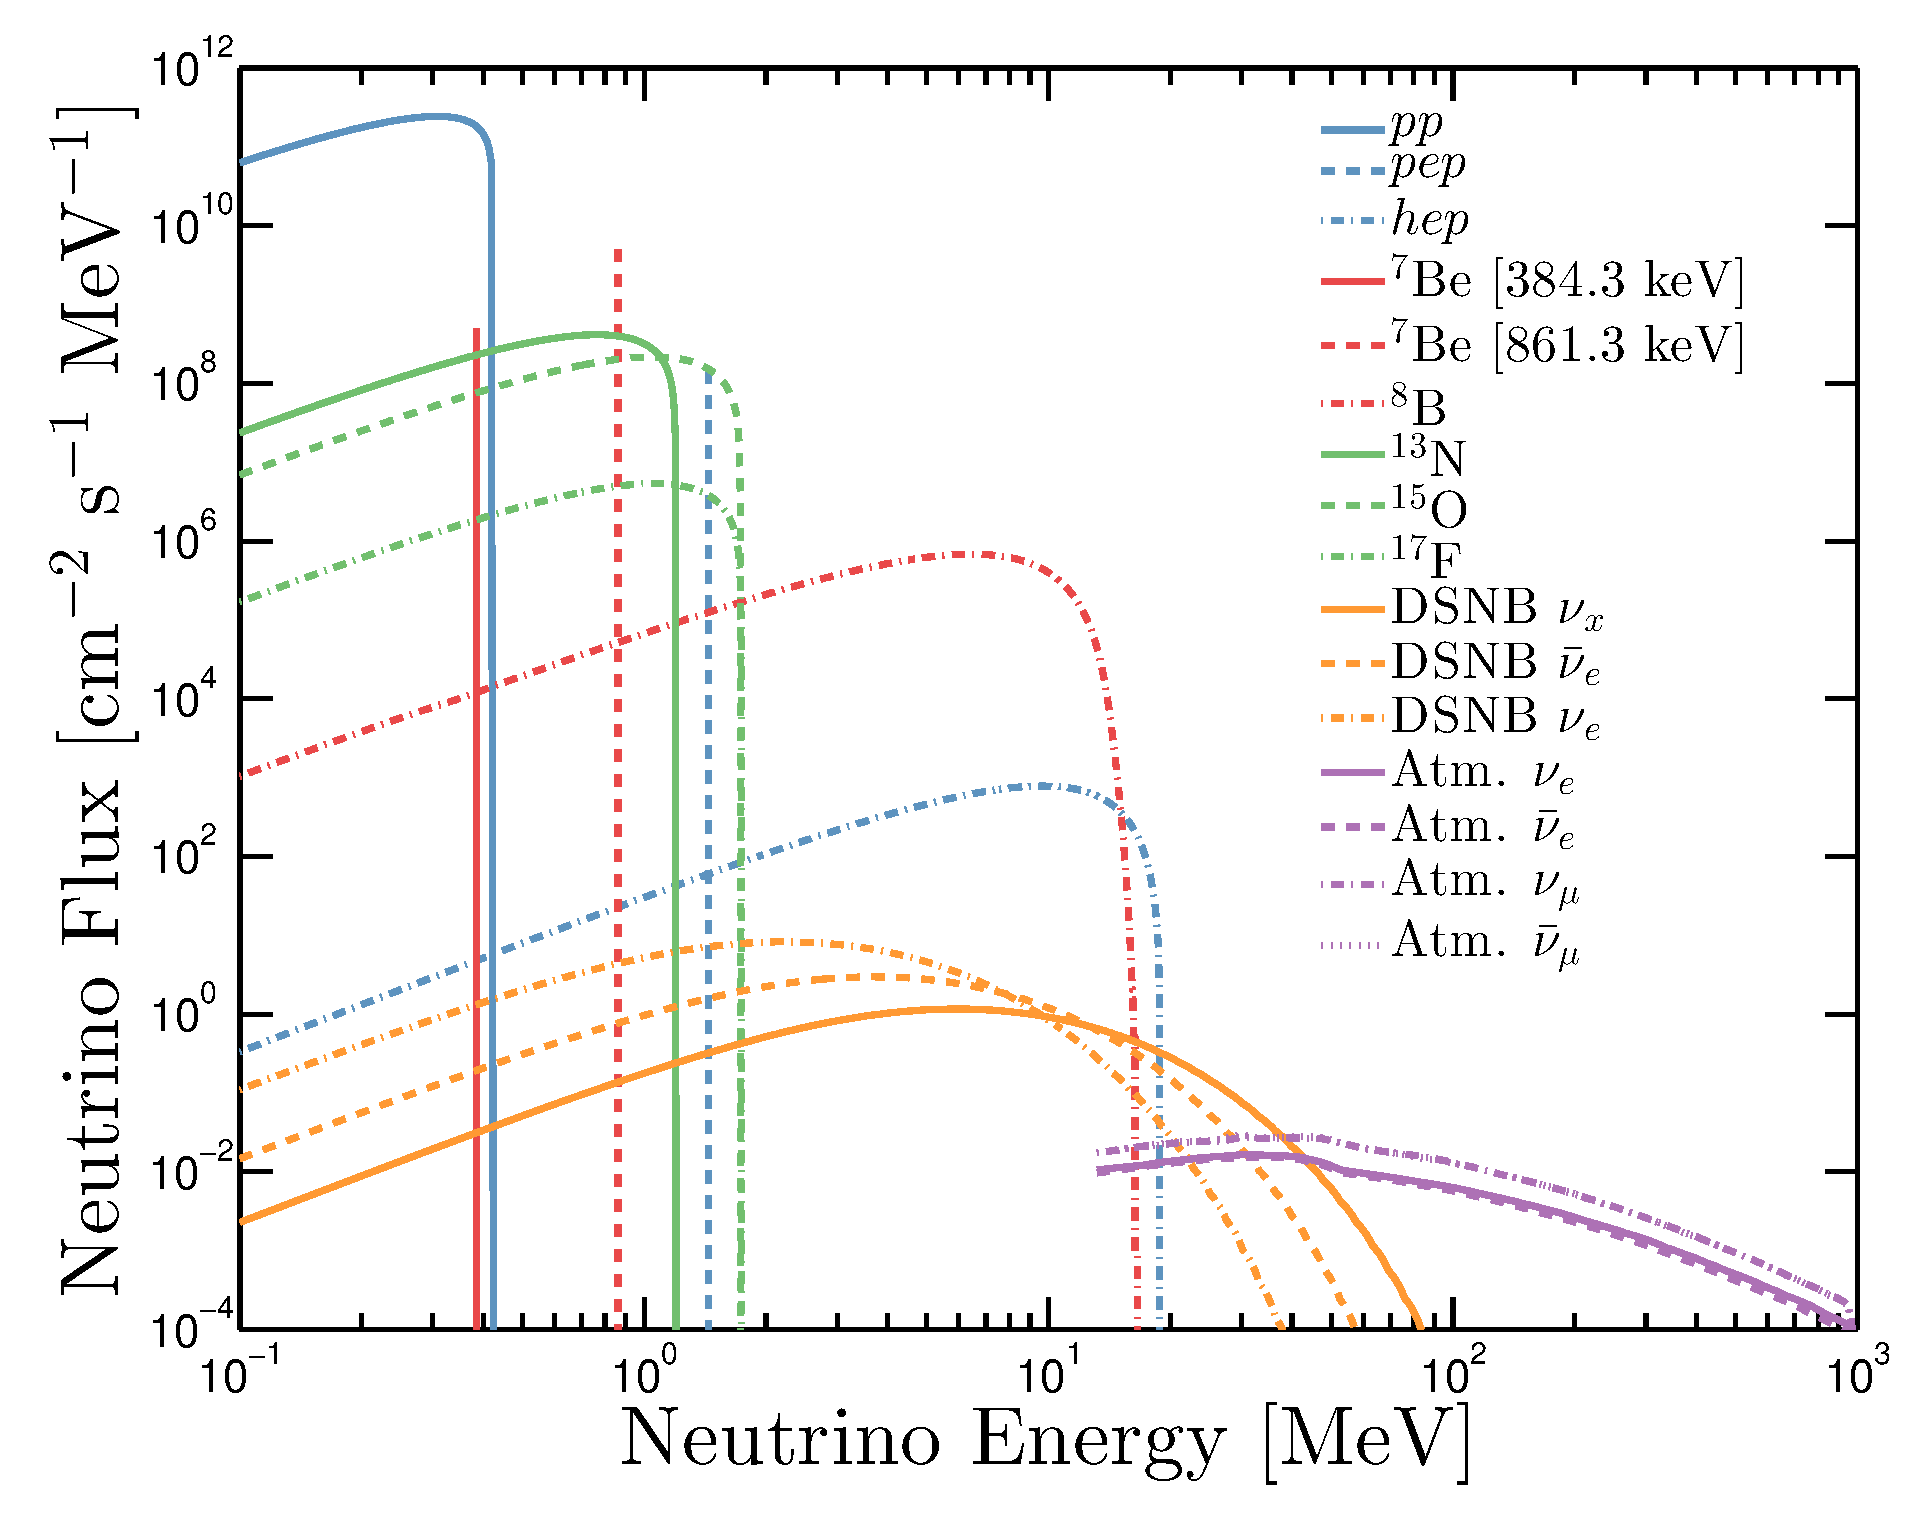
\includegraphics[trim = 5mm 0 0mm 3mm, clip, width=0.8\textwidth,angle=0]{Figures/neutrino_flux.eps}
\caption[Fluxes for neutrino backgrounds]{Neutrino energy spectra that are backgrounds to direct detection experiments: Solar, atmospheric, and the diffuse supernovae background (DSNB).} 
\label{fig:Flux}
\end{center}
\end{figure} 

\begin{table}[t]\centering
\ra{1.3}
\begin{tabularx}{\textwidth}{cc|cc|Y}
\hline\hline
$\mathbf{\nu}$ \bf{type} &  & $\mathbf{E_{\nu}^{\rm{max}}}$ \bf{(MeV)} & $\mathbf{E_{r_{\rm{Xe}}}^{\rm{max}}}$ \bf{(keV)} & $\Phi\pm \delta\Phi$ $\mathbf{(\rm{cm^{-2} \, s^{-1}})}$\\
\hline
\multirow{8}{*}{\bf Solar} &$pp$ & 0.42341 & $2.94\times 10^{-3}$ & $\left(5.98\pm 0.036 \right) \times 10^{10}$\\
&${}^{7}\rm{Be}$ & 0.8613 & 0.0122 & $\left( 5.00\pm 0.35 \right) \times 10^9$\\
&$pep$ & 1.440 & 0.0340 & $\left( 1.44\pm 0.017\right) \times 10^8$\\
&${}^{13}\rm{N}$ & 1.199 & 0.02356 & $\left(2.96\pm 0.41\right) \times 10^8 $\\
&${}^{15}\rm{O}$ & 1.732 & 0.04917 & $\left(2.23\pm 0.34\right) \times 10^8$\\
&${}^{17}\rm{F}$ & 1.740 & 0.04962 & $\left(5.52\pm 0.94 \right) \times 10^6$\\
&${}^{8}\rm{B}$ & 16.360 & 4.494 & $\left(5.16\pm 0.11\right) \times 10^6$\\
&$hep$ & 18.784 & 5.7817 & $\left( 8.04\pm 2.41 \right) \times 10^3$\\
\hline
\multirow{3}{*}{\bf DSNB}&$\nu_e$  &  &  & \\
&$+\bar{\nu}_e$  & $>$91.201 & $>$136.1 & $ 85.7\pm 42.7$\\
&$+\nu_x$  &  & & \\
\hline
\multirow{4}{*}{{\bf Atm.}}& $\nu_e$ & \multirow{4}{*}{$>$981.748} & \multirow{4}{*}{$>15.55\times 10^3$} & \multirow{4}{*}{$10.54\pm 2.1$}\\
&$+\bar{\nu}_e$ & &  &\\
&$+\nu_\mu$ &  &  &\\
&$+\bar{\nu}_\mu$ &  & & \\
\hline \hline
\end{tabularx}
\caption[Total neutrino fluxes with corresponding uncertainties]{Total neutrino fluxes with corresponding uncertainties. All solar neutrino fluxes are from the updated high metallicity SSM (Ref.~\cite{Serenelli:2011py}) with the exception of $^8$B which is from an analysis of neutrino data (Ref.~\cite{Bergstrom:2016cbh}). The DSNB and atmospheric neutrino fluxes are from Refs.~\cite{Beacom:2010kk} and~\cite{Honda:2011nf} respectively. The maximum neutrino energy, $E_{\nu}^{\rm{max}}$, and maximum recoil energy for a xenon target, $E_{r_{\rm{Xe}}}^{\rm{max}}$, are also shown. For atmospheric neutrinos and the DSNB we indicate the maximum neutrino energy used, though these fluxes in principle extend to higher energies.\label{tab:neutrino}}
\end{table}


To begin we describe the Solar, atmospheric and diffuse supernovae background neutrinos (DSNB) which scatter with nuclei into energies relevant for direct detection experiments. We expand upon previous results in the literature by highlighting the angular dependence of these fluxes. We display the energy spectra for each source of neutrino in Fig.~\ref{fig:Flux} and list each flux normalisation, $\Phi$, and uncertainty, $\delta \Phi$, in Table~\ref{tab:neutrino}.

{\bf Solar neutrinos} from nuclear fusion reactions in the interior of the Sun dominate the low energy-high flux regime and are the major neutrino background for direct detection with a total flux at Earth of $6.5\times10^{11}$~cm$^{-2}$~s$^{-1}$~\cite{Robertson:2012ib,Antonelli:2012qu}. Neutrinos from the initial proton-proton fusion reaction ``$pp$'' make up 86\% of the Solar emission and have been detected most recently by the Borexino experiment, which determined the flux with an uncertainty of $\sim 10$\% ~\cite{Bellini:2014uqa}. Despite the huge flux of $pp$ neutrinos they yield nuclear recoil energies well below the threshold of any direct detection experiment\footnote{$pp$ neutrinos would however be the dominant source of electron recoils.}. Secondary fusion of $p+e^-+p$ and $^3 $He$~+~p$ produce neutrinos, labelled ``$pep$'' and ``$hep$'', extend to energies beyond $pp$ neutrinos but with much lower flux. Shown in Fig.~\ref{fig:Flux} as lines are the two fluxes of monoenergetic neutrinos associated with $^7$Be electron capture. The lines have energies of 384.3~keV and 861.3~keV with branching ratios of $\sim$10\% and $\sim$90\% respectively. The latter of these is principally responsible for limiting the discovery for $m_\chi<1$~GeV so may become important in future ultra-low threshold light WIMP searches~\cite{Strigari:2016ztv}. In the following we ignore the Doppler broadening of these lines, as well as the $pep$ line, which would induce a negligible correction to the subsequent recoil energy spectrum. Next we have neutrinos due to the decay of $^8$B which extend up to $\sim$10 MeV in energy placing them within the reach of dark matter searches. The spectrum of $^8$B neutrinos mimics the signal from a WIMP with a mass of 6~GeV and will likely be the first to be detected (via nuclear recoils) in future direct detection experiments. Finally we have neutrinos arising from the carbon-nitrogen-oxygen (CNO) cycle labelled by the decay from which they originate: $^{13}$N, $^{15}$O and $^{17}$F. These are at present unmeasured but Borexino places an upper bound of $<7.7\times10^8$~cm$^{-2}$~s$^{-1}$ on the sum of their flux~\cite{Bellini:2013lnn}. CNO neutrinos are a subdominant background for us but are of great interest to studies of stellar physics since their flux is highly sensitive to the Solar metallicity. 

The theoretical systematic uncertainties on the Solar neutrino fluxes range from 1\% ($pp$ flux) to 14\% ($^8$B flux). Although out of these various components, four have now been directly measured: $pp$, $pep$, $^8$B and $^7$Be. For all except $^8$B, the theoretical uncertainty is smaller than the measurement uncertainty. The theoretical uncertainty arises largely from the uncertainty in the Solar metallicity, and in order to establish a self-consistent model of Solar neutrino fluxes one must assume a metallicity model. The Standard Solar models (SSMs) of Grevesse \& Sauval~\cite{Grevesse:1998bj} are broadly split into two categories `high-Z' and `low-Z' based on the assumed Solar metallicity,~Z. Both models have historically disagreed with some set of observables such as neutrino data, helioseismology or surface helium abundance~\cite{Villante:2013mba}. To remain consistent with previous neutrino floor calculations (e.g. Ref.~\cite{Ruppin:2014bra}) we consider the high-Z model. We use values presented in Ref.~\cite{Serenelli:2011py} which are based on updated fusion cross sections~\cite{Adelberger:2010qa}. The most recent generation of SSMs from Vinyoles~\etal~\cite{Vinyoles:2016djt} have a mild preference towards a high-Z configuration, though the authors note that neither are free from some level of disagreement with the various Solar observables\footnote{Dark matter detection experiments may shed further light on the Solar metallicity issue, e.g. Refs.~\cite{Billard:2014yka,Strigari:2016ztv,Cerdeno:2016sfi}. The measurement of CNO neutrinos will be essential for this, and may be possible in the future for instance with a neon target experiment as suggested by Ref.~\cite{Cerdeno:2016sfi}.}. We set our systematic uncertainties on each flux to the theoretical estimate with the exception of $\delta \Phi_{^8{\rm B}}$ for which the measurement uncertainty is smaller; we use the result presented in Ref.~\cite{Bergstrom:2016cbh} based on a global analysis of all Solar and terrestrial neutrino data. 

In addition to the spectra and flux of Solar neutrinos, we are also interested in their direction and time dependence. Due to the eccentricity of the Earth's orbit, the Earth-Sun distance has an annual variation leading to a modulation in the Solar neutrino flux as seen by an Earth-based experiment such that,
\begin{equation}
  \frac{\textrm{d}^2 \Phi(t)}{\textrm{d}E_\nu \textrm{d}\Omega_\nu}  =  \frac{\textrm{d} \Phi}{\textrm{d} E_\nu} \,\left[ 1 + 2 e \cos\left(\frac{2\pi(t- t_\nu)}{T_\nu}\right) \right] 
 \delta\left(\hat{{\bf q}}_\nu-\hat{{\bf q}}_\odot(t)\right) \,,
\label{eq:solarneutrinoflux_directional}
\end{equation}
where $t$ is the time from January 1st, $e = 0.016722$ is the eccentricity of the Earth's orbit, $t_{\nu} = 3$ days is the time at which the Earth-Sun distance is minimum (and hence the Solar neutrino flux is largest), $T_{\nu} = 1$ year, $\hat{{\bf q}}_{\nu}$ is a unit vector in the direction of interest and $\hat{{\bf q}}_\odot(t)$ is a unit vector in the inverse of the direction towards the Sun\footnote{We ignore the angular size of the Sun's core on the sky which would cause a tiny angular spread in the incoming neutrino directions, see e.g. Ref.~\cite{Davis:2016hil}.}. This annual modulation has been observed most recently in $^7$Be neutrinos by Borexino~\cite{Agostini:2017iiq}.


{\bf Atmospheric neutrinos} due to cosmic ray collisions are responsible for the neutrino floor for WIMP masses around $\sim$100 GeV and will limit the discovery of SI cross sections below approximately $10^{-48}$ cm$^2$~\cite{Strigari:2009bq,Billard:2013qya,Ruppin:2014bra}. The flux of atmospheric neutrinos at the relevant low energies ($\sim$100 MeV) is difficult to both measure and theoretically predict~\cite{Battistoni:2005pd} so currently has uncertainties of around 20\%~\cite{Honda:2011nf}.

\begin{figure}
\begin{center}
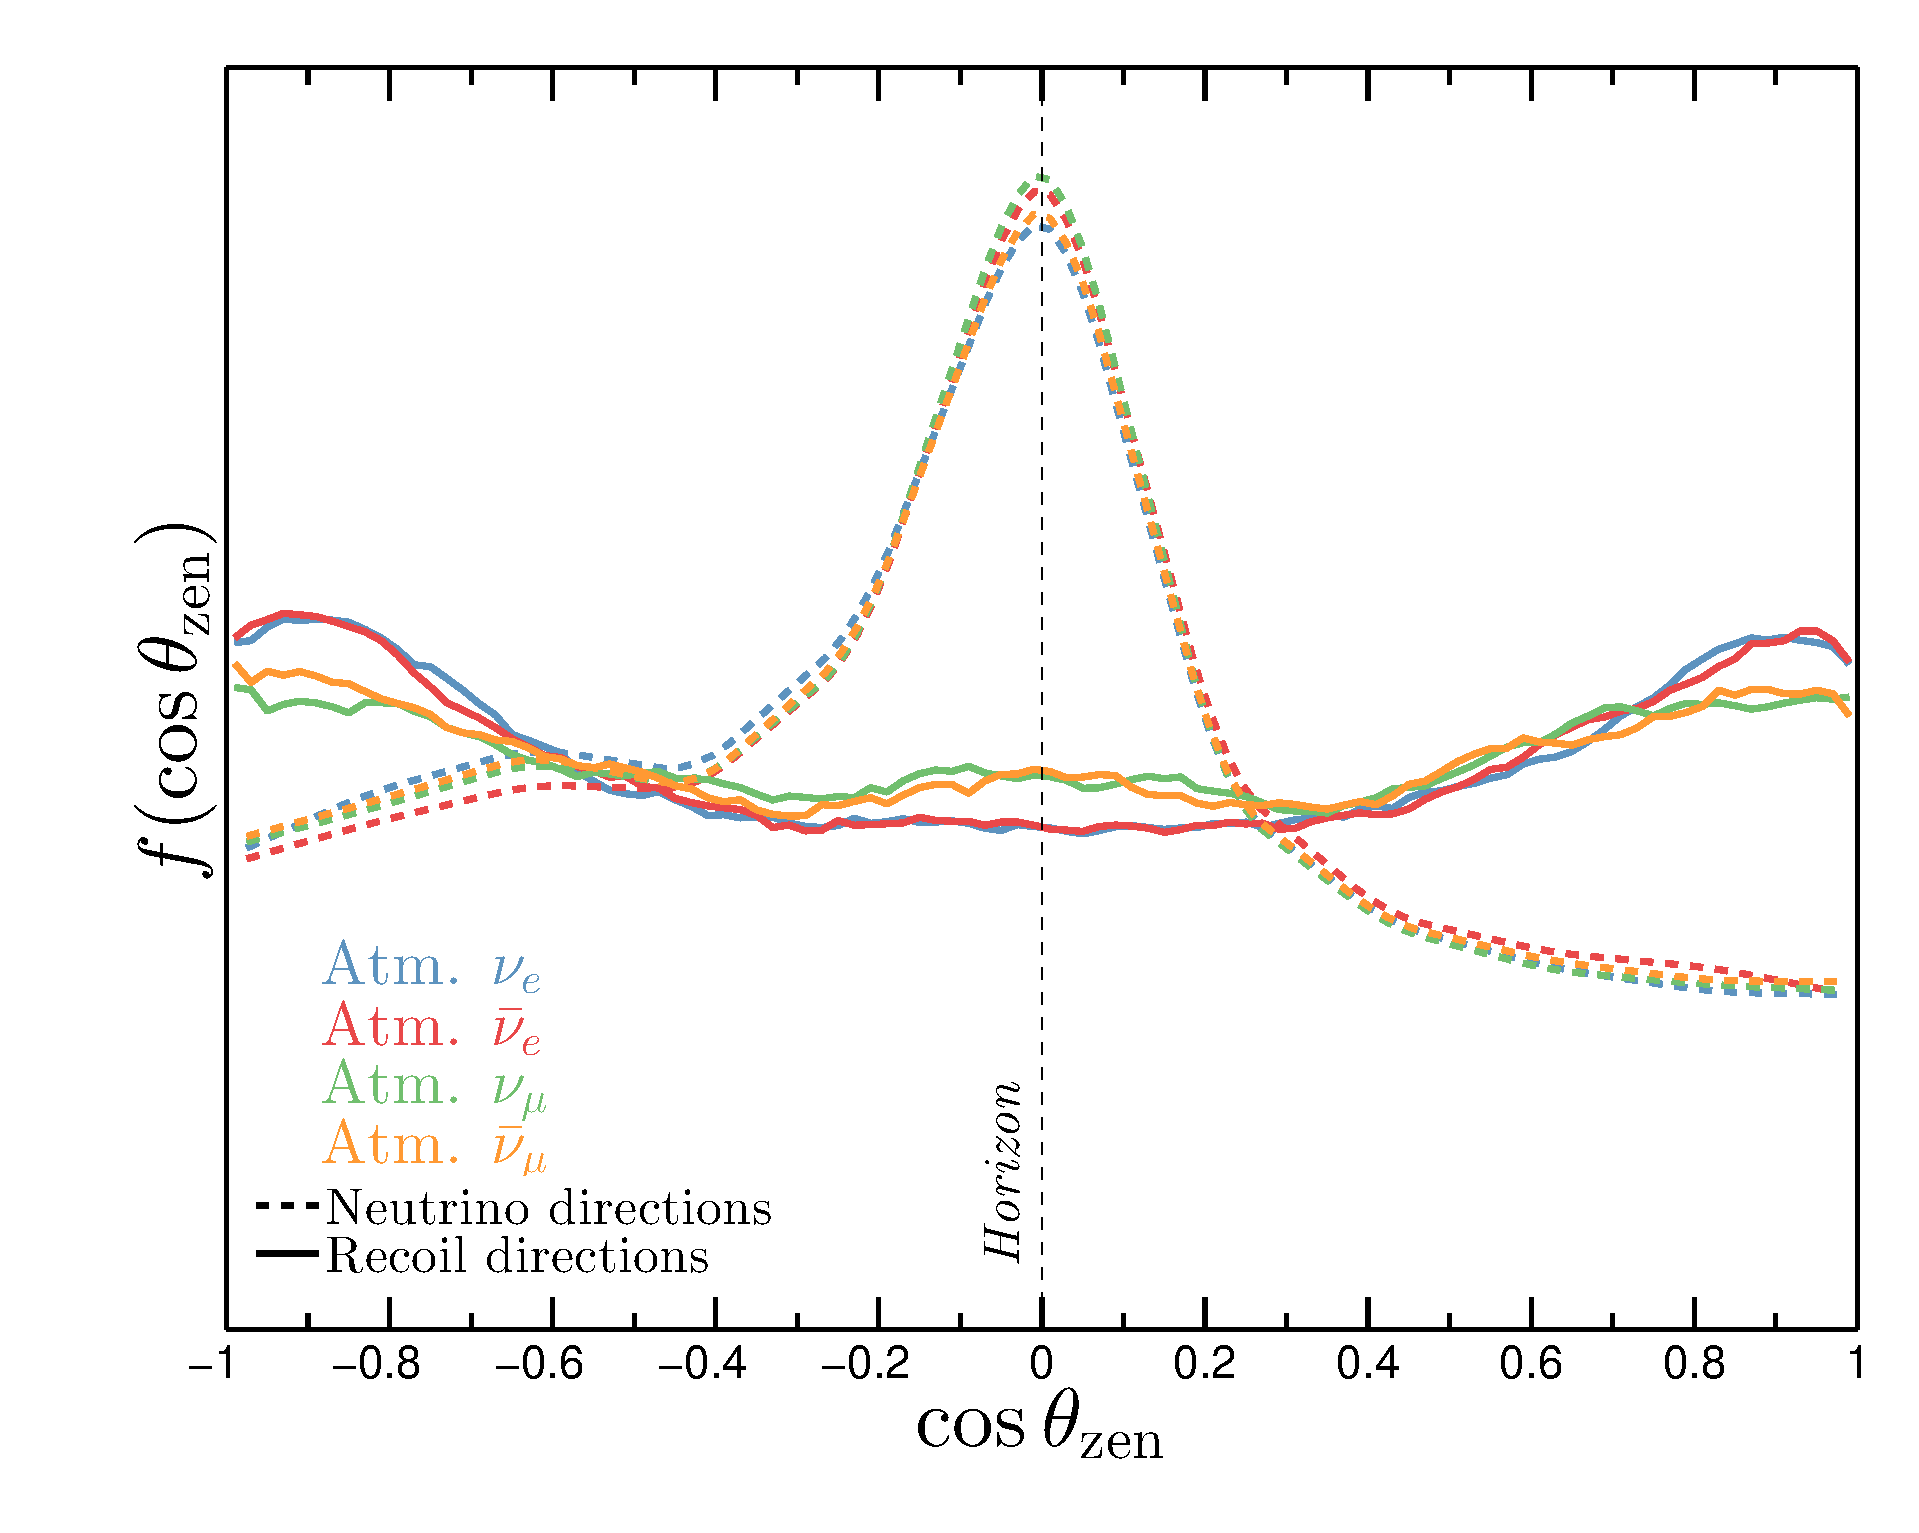
\includegraphics[trim = 0mm 0 0mm 0mm, clip, width=0.8\textwidth,angle=0]{Figures/AtmNu_zenith.eps}
\caption[Atmospheric neutrino directionality]{Angular distributions of atmospheric neutrino and their subsequent recoils. We show distributions as a function of zenith angle $\theta_{\rm zen}$ for incoming neutrinos (dashed lines) and xenon recoils above $E_{\rm th} = 5$ keV (solid lines) generated using a Monte-Carlo scattering simulation (Appendix~\ref{app:scattering}). The four lines in each case correspond to the four species of atmospheric neutrino, $\nu_e$ (blue lines), $\bar{\nu}_e$ (red lines), $\nu_\mu$ (green lines), $\bar{\nu}_\mu$ (orange lines). The incoming neutrino directions are based on the FLUKA simulations~\cite{Battistoni:2005pd}.} 
\label{fig:FLUKA}
\end{center}
\end{figure} 
Over all energies, the atmospheric neutrino flux peaks near the horizon, at zenith angle $\cos\theta_{\rm zen} \approx 0$. At high energies, the flux is very nearly symmetric about $\cos \theta_{\rm zen} \approx 0$, as at these energies the cosmic ray particles are more energetic than the rigidity cutoff. At low energies, the flux becomes asymmetric, as the flux of downward-going ($\cos \theta_{\rm zen} = 1$) neutrinos is lower than the flux of upward-going neutrinos ($\cos \theta_{\rm zen} = -1$). We consider the FLUKA results for the angular dependence of the atmospheric neutrino flux at energies relevant for direct detection experiments~\cite{Battistoni:2002ew}. In Fig.~\ref{fig:FLUKA} we show the angular spectrum of the atmospheric neutrino flux which exhibits the aforementioned dependence on zenith angle. The flux is assumed to be symmetric with azimuthal angle.

As we will discuss below we find that when the flux of atmospheric neutrinos is convolved with the coherent neutrino-nucleus scattering cross section, the angular dependence becomes washed out and the recoil spectrum depends only weakly on direction (when compared with other neutrino components and particularly WIMP recoils). Because this angular dependence is close to isotropic and will not undergo the characteristic daily transit across the sky due to the rotation of the Earth, including it will not greatly affect the discrimination between atmospheric neutrinos and WIMPs. In principle there should be a seasonal variation in the neutrino flux based on the atmospheric temperature which induces an additional time modulation, e.g. Ref.~\cite{Tilav:2010hj}. However the exact time dependence of this effect at the location of our mock experiment (Modane Underground Laboratory, France) is not known. Furthermore these variations appear to be smaller than either the WIMP or Solar neutrino modulation which are already very small effects. Hence for our analysis we model the atmospheric flux as both isotropic and constant in time,
\begin{equation}
  \frac{\textrm{d}^2 \Phi}{\textrm{d}E_\nu \textrm{d}\Omega_\nu} = \frac{1}{4\pi}\frac{\textrm{d} \Phi}{\textrm{d} E_\nu}  \,.
\label{eq:ATMDSNBflux}
\end{equation}



{\bf Diffuse supernova neutrinos}: For WIMP masses between 10 and 30 GeV, the neutrino floor is induced by the subdominant diffuse supernova neutrino background (DSNB), from all supernova explosions in the history of the Universe. The DSNB flux is the integral of the rate density for core-collapse supernova $R_{\rm SN}$ as a function of redshift $z$, with the neutrino spectrum per supernova $\Phi_{\rm SN}$~\cite{Beacom:2010kk},
\begin{equation}
 \frac{\textrm{d}\Phi}{\textrm{d}E_\nu} = \int_0^\infty \left[(1+z) \Phi_{\rm SN}(E_\nu(1+z))\right]\left[R_{\rm SN}(z)\right] \bigg|\frac{\textrm{d}t}{\textrm{d}z}\bigg| \textrm{d}z \, .
\end{equation}
where $|\textrm{d}t/\textrm{d}z|^{-1} = H_0(1+z)[\Omega_\Lambda + \Omega_m(1+z)^3]^{1/2}$ is the differential `look-back' time. The resulting spectra have a roughly Fermi-Dirac form with temperatures in the range 3~-~8~MeV. We use the following temperatures for each neutrino flavour given by Ref.~\cite{Beacom:2010kk}: $T_{\nu_e}~=~3$~MeV, $T_{\bar{\nu}_e}~=~5$~MeV and $T_{\nu_x}~=~8$~MeV, where $\nu_x$ represents the four remaining neutrino flavours. Motivated by theoretical estimates we take a systematic uncertainty on the DSNB flux of 50\%. The DSNB is believed to be isotropic and constant over time, therefore its angular dependence can be expressed, as with the atmospheric neutrinos, using Eq.~(\ref{eq:ATMDSNBflux}).  


{\bf Other neutrinos}: We have summarised the three sources of neutrino that are most important for the discovery limits of dark matter experiments, although there are a few sources we do not consider. Most notably neutrinos from individual Milky Way supernovae would also certainly show up in direct detection experiments if the explosion were close enough to Earth. In fact existing and future ton-scale detectors are in a position to perform novel supernova physics in the event of a Galactic supernova~\cite{Lang:2016zhv}. We do not consider distinct supernovae neutrinos as a background here as the events would probably be coincident with a large nearby explosion.

We do not need to consider cosmological relic neutrinos as their energies are well below the thresholds of all current and near future experiments, however we note that the motion of the Milky Way with respect to the rest frame of the CMB would give rise to a signature direction dependence as with the primary CMB dipole~\cite{Safdi:2014rza,Domcke:2017aqj}.
We also neglect reactor neutrinos as it is unlikely that a direct detection experiment would be situated close enough to a nuclear reactor for them to be a significant background. We also ignore sources of geoneutrinos from radioactive decays which produce a subdominant flux from the ground with energies below 4.5 MeV~\cite{Monroe:2007xp}. Finally, fluxes of much higher energy extragalactic neutrinos from, for example, active galactic nuclei or gamma-ray bursts, have fluxes well below the sensitivity of a dark matter experiment~\cite{Gaisser:1994yf,Halzen:2002pg,Aartsen:2014gkd}.



\subsection{Coherent neutrino-nucleus elastic scattering}
We only consider the neutrino background from coherent neutrino-nucleus elastic scattering (CNS) as it produces nuclear recoils in the keV energy scale which cannot be distinguished from a WIMP interaction\footnote{We neglect neutrino-electron elastic scattering, mostly induced by $pp$ neutrinos, as it has been shown to only marginally affect the discovery potential of experiments with limited nuclear/electronic recoil discrimination for WIMP masses above 100 GeV~\cite{Billard:2013qya}.}. CNS proceeds via a neutral current, and as shown by Freedman~\cite{Freedman:1973yd} and subsequently Drukier \& Stodolsky~\cite{Drukier:1983gj} has a coherence effect at low momentum transfer that approximately scales with the number of neutrons squared. At higher recoil energies, generally above a few tens of keV, the loss of coherence is described by the nuclear form factor $F(E_r)$, for which we again use the standard Helm ansatz~\cite{Lewin:1995rx} which is an excellent approximation at these low energies~\cite{Vietze:2014vsa}. The differential cross section as a function of the nuclear recoil energy ($E_r$) and neutrino energy ($E_\nu$) is given by 
\be
  \frac{\textrm{d} \sigma}{\textrm{d}E_r}(E_r,E_\nu) = \frac{G_F^2}{4 \pi} Q^2_W m_N \left(1-\frac{m_N E_r}{2 E_\nu^2} \right) F^2(E_r) \,,
\ee
where $Q_W = A-Z - (1-4\sin^2\theta_W) Z$ is the weak nuclear hypercharge of the nucleus, $G_F$ is the Fermi coupling constant, $\theta_W$ is the weak mixing angle and $m_N$ is the target nucleus mass. We assume CNS to be a pure standard model interaction and do not consider any exotic mediators as in, for example, Refs.~\cite{Cerdeno:2016sfi,Bertuzzo:2017tuf}.

The directional cross section can be written by noting that the scattering has azimuthal symmetry about the incoming neutrino direction so $\rm{d}\Omega_\nu = 2\pi \,\rm{d}\cos\beta$ and imposing the kinematical expression for the scattering angle, $\beta$, between the neutrino direction, $\hat{{\bf q}}_\nu$, and the recoil direction, $\hat{{\bf q}}_r$,
\be
 \cos\beta = \hat{{\bf q}}_r \cdot \hat{{\bf q}}_\nu = \frac{E_\nu + m_N}{E_\nu}\sqrt{\frac{E_r}{2 m_N}} \,,
\label{eq:kinematics}
\ee 
with $\beta$ in the range $(0,\pi/2)$, using a delta function,
\be
  \frac{\textrm{d}^2 \sigma}{\textrm{d}E_r \textrm{d}\Omega_r} = \frac{\textrm{d} \sigma}{\textrm{d}E_r} \, \frac{1}{2 \pi}\, \delta\left(\cos\beta - \frac{E_\nu + m_N}{E_\nu} \sqrt{\frac{E_r}{2 m_N}}\right) \,.
\label{eq:doublecrosssection}
\ee
The maximum recoil energy, $E_r^{\rm max}$, can be obtained by setting $\beta = 0$ in Eq.~(\ref{eq:kinematics}),
\be
E_r^{\rm max} = \frac{2 m_N E_\nu^2}{(E_\nu + m_N)^2} \approx \frac{2E_\nu^2}{m_N + 2E_\nu} \,.
\ee
The maximum recoil energies produced by the different types of neutrino for a xenon target are shown in Table~\ref{tab:neutrino}.

\par The CNS event rate per unit detector mass, as a function of the recoil energy, direction and time, is given by the convolution of the double differential CNS cross section and the directional neutrino flux,
\be\label{eq:nu_directionalrate}
  \frac{\textrm{d}^2 R(t)}{\textrm{d}E_r \textrm{d}\Omega_r} =  \frac{1}{m_N} \int_{E_\nu^{\rm min}} \frac{\textrm{d}^2 \sigma}{\textrm{d}E_r \textrm{d}\Omega_r}\times\frac{\textrm{d}^2 \Phi(t)}{\textrm{d}E_\nu \textrm{d}\Omega_\nu} \textrm{d}E_\nu \textrm{d}\Omega_\nu \,,
\ee
where $E_\nu^{\rm min} = \sqrt{m_NE_r/2}$ is the minimum neutrino energy required to generate a nuclear recoil with energy $E_r$.

The directional event rate for Solar neutrinos is found by substituting Eqs.~(\ref{eq:solarneutrinoflux_directional}), (\ref{eq:kinematics}) and (\ref{eq:doublecrosssection}) into Eq.~(\ref{eq:nu_directionalrate}) and integrating over the neutrino direction $\Omega_\nu$,
\begin{align}
  \frac{\textrm{d}^2 R(t)}{\textrm{d}E_r \textrm{d}\Omega_r} &= \frac{1}{2\pi m_N}\left[ 1 + 2\epsilon\cos\left(\frac{2\pi(t- t_\nu)}{T_\nu}\right) \right]  \nonumber \\
&\times \int \frac{\textrm{d} \sigma}{\textrm{d}E_r}  \frac{\textrm{d} \Phi}{\textrm{d} E_\nu} \delta\left(\hat{{\bf q}}_r \cdot \hat{{\bf q}}_\odot(t) - \frac{E_\nu + m_N}{E_\nu} \sqrt{\frac{E_r}{2 m_N}}\right) \textrm{d}E_\nu \,.
\label{eq:intermediate}
\end{align}
The delta function can then be rewritten as
\be
  \delta\left(\hat{{\bf q}}_r \cdot \hat{{\bf q}}_\odot(t) - \frac{E_\nu + m_N}{E_\nu} \sqrt{\frac{E_r}{2 m_N}}\right) =  \frac{1}{E_\nu^\textrm{min}} \, \,\delta \left(x + \frac{1}{\mathcal{E}(t)}\right) \, ,
\label{eq:delta}
\ee
where we have defined $x = -1/E_\nu$ and,
\be
  \frac{1}{\mathcal{E}(t)} = \frac{\hat{{\bf q}}_r \cdot \hat{{\bf q}}_\odot(t)}{E_\nu^\textrm{min}} - \frac{1}{m_N} \,.
\ee

Finally, by substituting Eq.~(\ref{eq:delta}) into Eq.~(\ref{eq:intermediate}), integrating over $x$ and converting back to $E_\nu$, we obtain an analytic expression for the directional event rate from Solar neutrinos,
\begin{equation}
  \frac{\textrm{d}^2 R(t)}{\textrm{d}E_r \textrm{d}\Omega_r} =  \frac{1}{2\pi m_N}\left[ 1 + 2\epsilon\cos\left(\frac{2\pi(t- t_\nu)}{T_\nu}\right) \right]  \frac{\mathcal{E}(t)^2}{ E_\nu^\textrm{min}} \left(\frac{\textrm{d} \sigma}{\textrm{d}E_r}\frac{\textrm{d} \Phi}{\textrm{d} E_\nu}\right)\bigg|_{E_\nu = \mathcal{E}(t)} \,,
\label{eq:solarnu}
\end{equation}
for $\cos^{-1}(\hat{{\bf q}}_r \cdot \hat{{\bf q}}_\odot(t)) < \pi/2$ and 0 otherwise.

In the case of the atmospheric and diffuse supernova neutrinos, as we have assumed their fluxes to be isotropic and constant over time, the directional event rate is simply given by substituting Eqs.~(\ref{eq:ATMDSNBflux}) and (\ref{eq:doublecrosssection}) into Eq.~(\ref{eq:nu_directionalrate}) and integrating over the neutrino direction $\Omega_\nu$ leading to
\be
\frac{\textrm{d}^2 R}{\textrm{d}E_r \textrm{d}\Omega_r} = \frac{1}{4\pi m_N} \int_{E_{\nu}^\textrm{min}} \frac{\textrm{d} \sigma}{\textrm{d}E_r} \frac{\textrm{d} \Phi}{\textrm{d}E_\nu } \textrm{d}E_\nu \,. 
\label{eq:isonu}
\ee


\subsection{Resulting signals}
\label{sec:nufloor_signals}
 \begin{figure}
\begin{center}
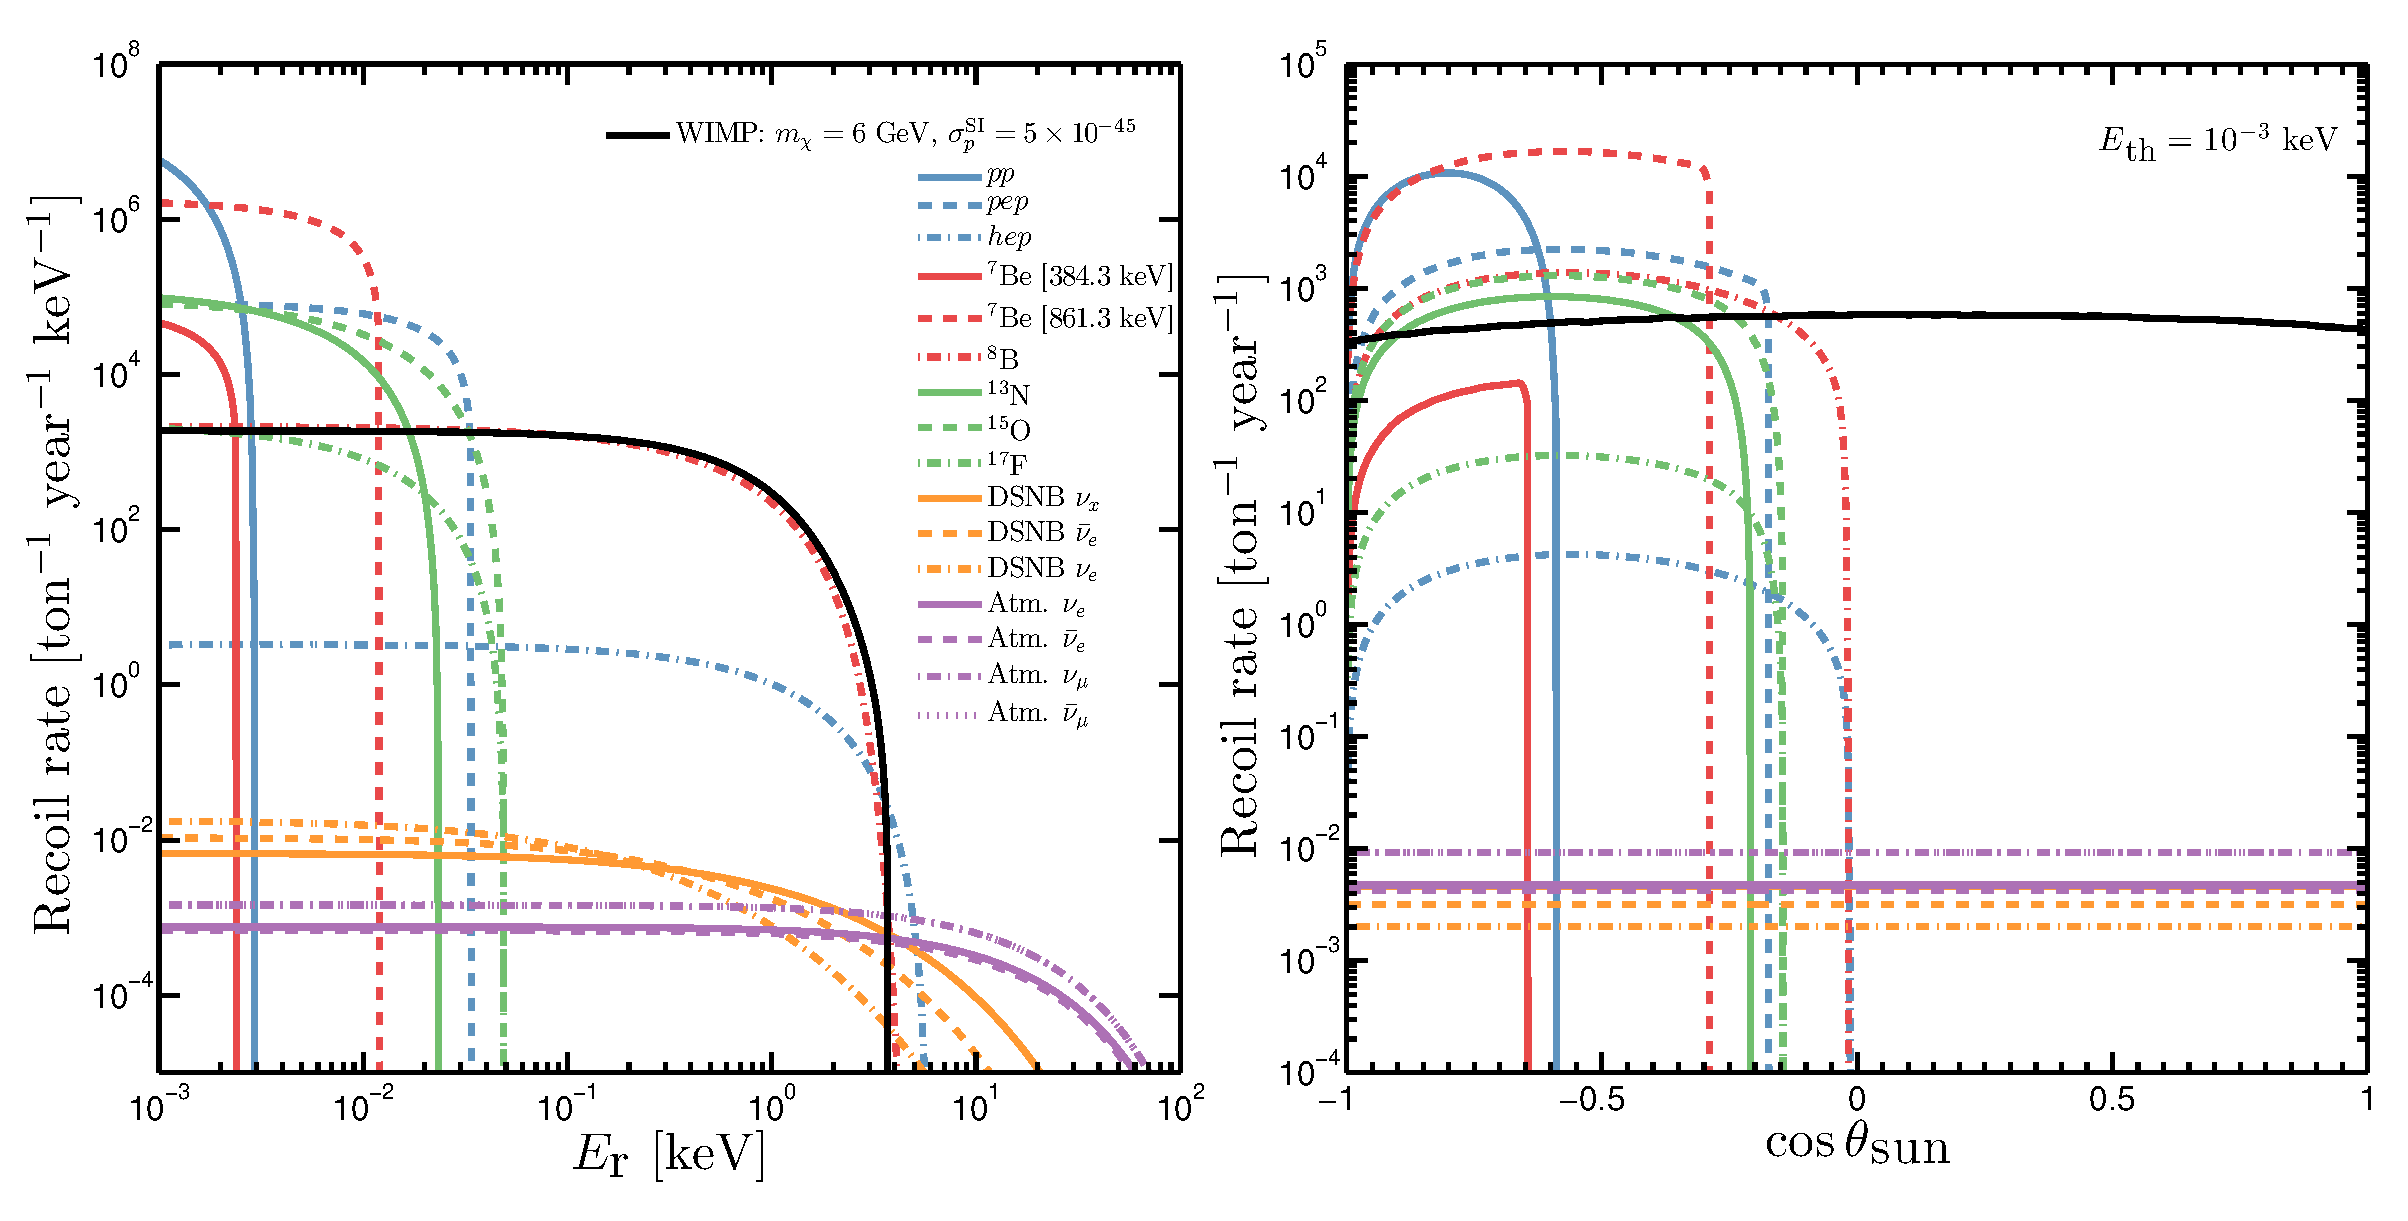
\includegraphics[trim = 0mm 0 0mm 0mm, clip, width=0.98\textwidth,angle=0]{Figures/NeutrinoAll_1D_recoilrates.eps}
\caption[Neutrino and $m_{\chi} = 6 \, {\rm GeV}$ WIMP nuclear recoil rates]{Neutrino and $m_{\chi} = 6 \, {\rm GeV}$ WIMP nuclear recoil rates for a xenon target as a function of recoil energy, $E_r$, (left) and cosine of the angle between the Solar vector and recoil vector, $\cos \theta_\textrm{sun}$, (right)  obtained by integrating the differential recoil spectrum over angle and energy respectively. The atmospheric and DSNB neutrino fluxes are taken to be isotropic. In order to show all types of neutrino we integrate above $E_r = 1$~eV.} 
\label{fig:neutrinorates}
\end{center}
\end{figure} 
The neutrino event rates as a function of energy and angle between Solar and recoil directions, $\cos{\theta_\textrm{sun}} = -\hat{\bf{q}}_r\cdot\hat{\bf{q}}_\odot$, obtained by integrating Eqs.~(\ref{eq:solarnu}) and ~(\ref{eq:isonu}) over direction and energy respectively are shown in Fig.~\ref{fig:neutrinorates}. Also shown is the recoil rate for a 6 GeV WIMP, showing the similarity between this spectrum and the spectrum of $^8$B neutrino recoils. The isotropic DSNB and atmospheric recoil rates are flat whereas the event rates of Solar neutrinos are highly anisotropic. The curves corresponding to the monoenergetic neutrinos ($^7$Be and $pep$) have a sharp cutoff in their directionality due to the finite energy threshold. From Fig.~\ref{fig:neutrinorates} one can already anticipate that the degeneracy between Solar neutrino and WIMP events from an energy-only analysis will be almost completely removed with the addition of directional information.


 \begin{figure}
\begin{center}
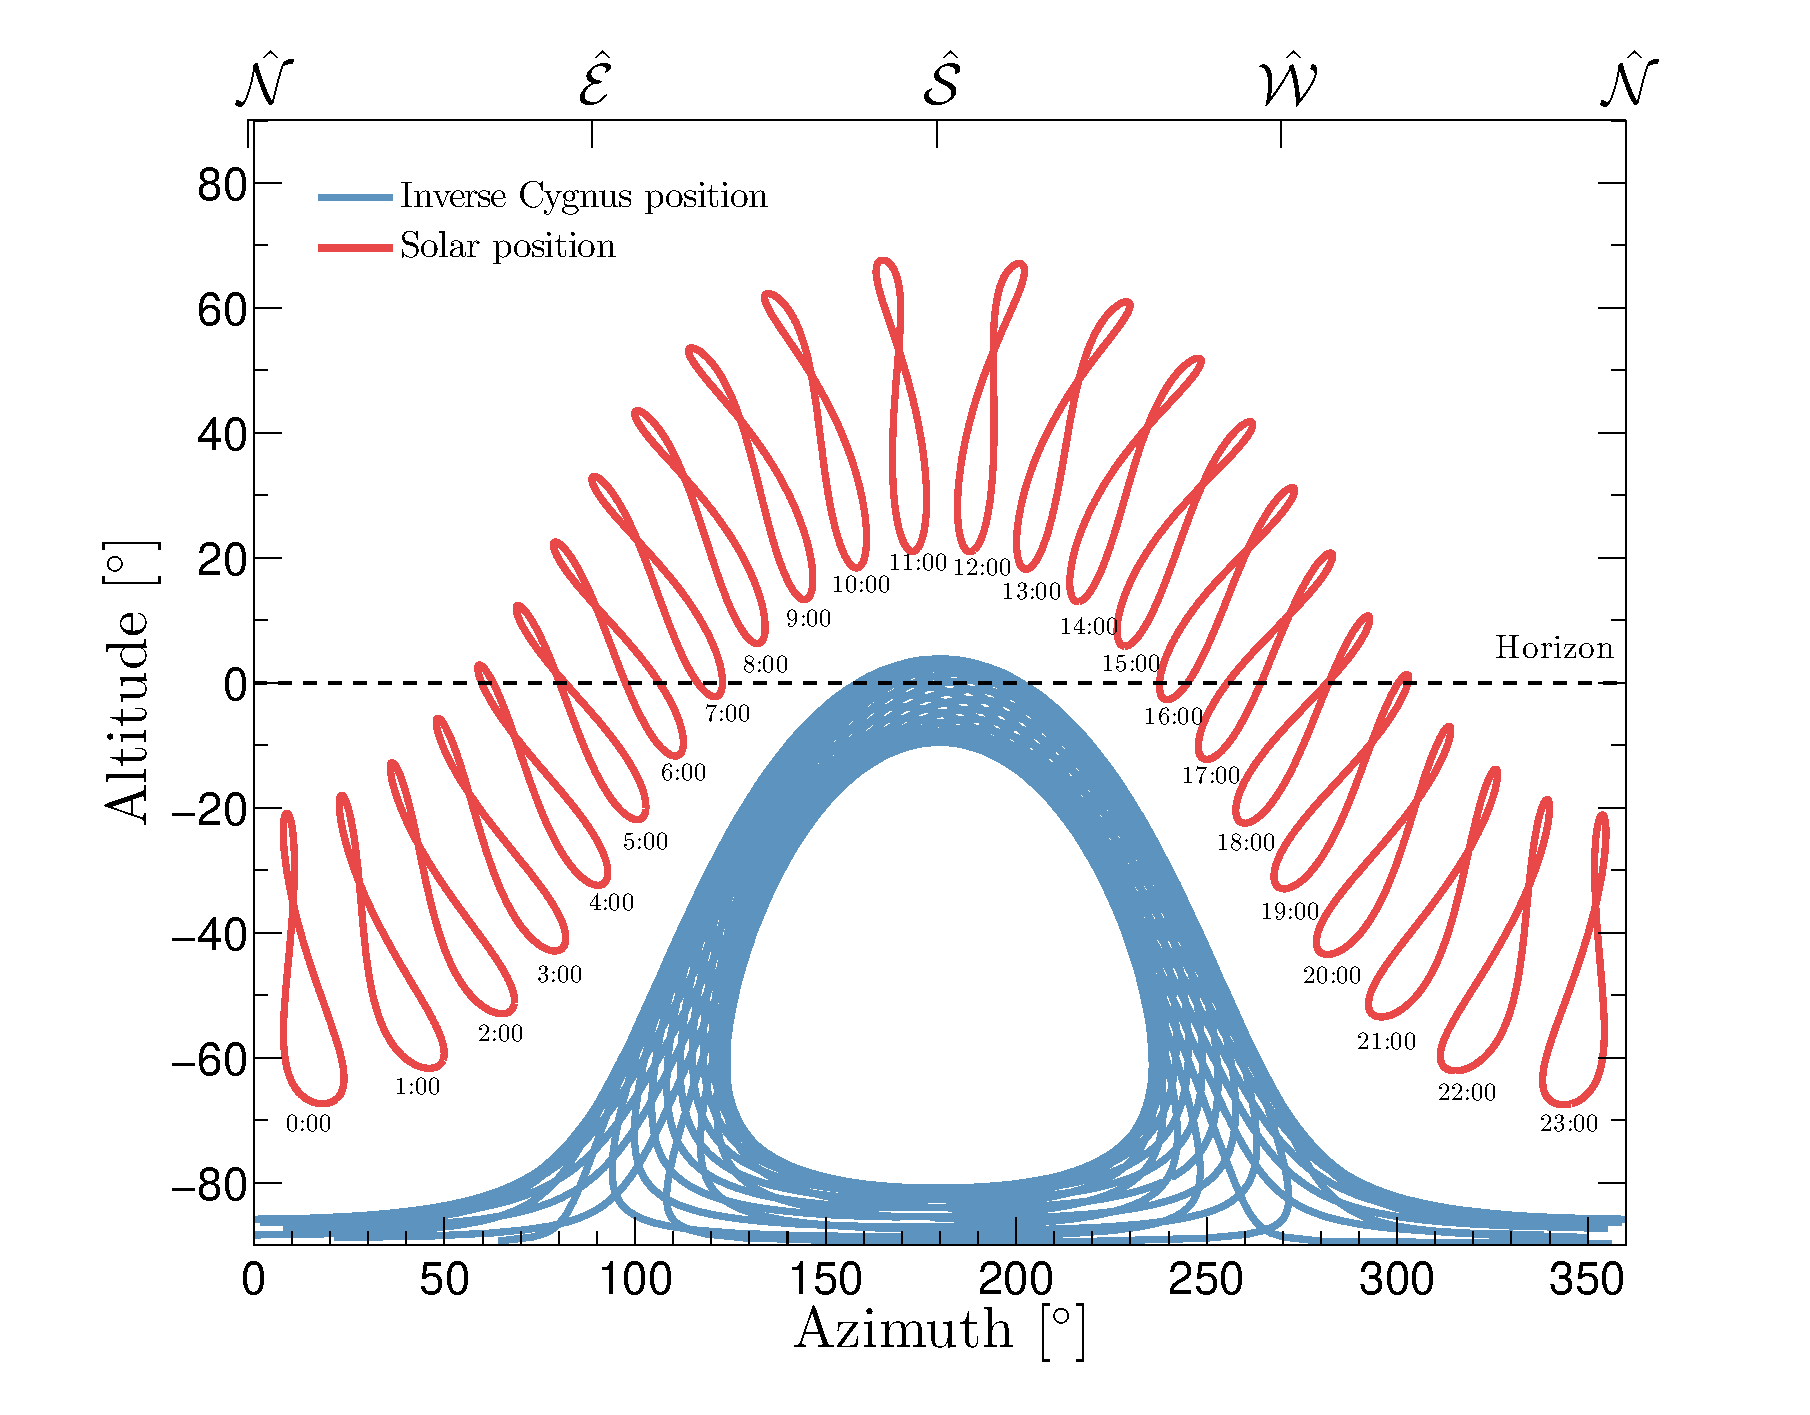
\includegraphics[trim = 15mm 5mm 18mm 5mm, clip, width=0.8\textwidth,angle=0]{Figures/SolarCygnusDirections.eps}
\caption[The evolution of the position of the Sun and Cygnus in the sky]{The position in the sky, in terms of Altitude and Azimuth, of the Sun (red) and the inverse of the position of the constellation Cygnus (corresponding to the direction -$\bf{v}_\textrm{lab}$) (blue) as observed from the Modane underground laboratory (latitude $45.2^{\circ}$). The points show the position at measurements made every hour from the 1st January 2015 0:00 until 31st December 2015 23:00. The Solar position traces out 24 analemmas for observations made at each hour of the day over the course of a year. The dashed horizontal line is the horizon. As demonstrated here, the Sun's position does not coincide with that of Cygnus at any time.} 
\label{fig:solarcygnus}
\end{center}
\end{figure} 
Figure~\ref{fig:solarcygnus} shows the position in the sky of the Sun and the inverse of the position of Cygnus (i.e. $-\bf{v}_\textrm{lab}$), as observed from the Modane underground laboratory (latitude $45.2^{\circ}$). The points show the position at observations made every hour from the 1st January 2015 0:00 until 31st December 2015 23:00. The Solar position traces out 24 `analemmas' which are lines connecting observations of the Sun's position at the same hour each day over a full year. As we see here, the Sun's position does not coincide with that of Cygnus at any time suggesting that a directional experiment should in principle be able to disentangle the WIMP from the Solar neutrino contributions in the observed data. In fact the angular separation between the peak WIMP direction and the peak neutrino direction undergoes a sinusoidal modulation over the course of the year that varies from $60^{\circ}$ in February to $120^{\circ}$ in September.

\begin{figure}
\begin{center}
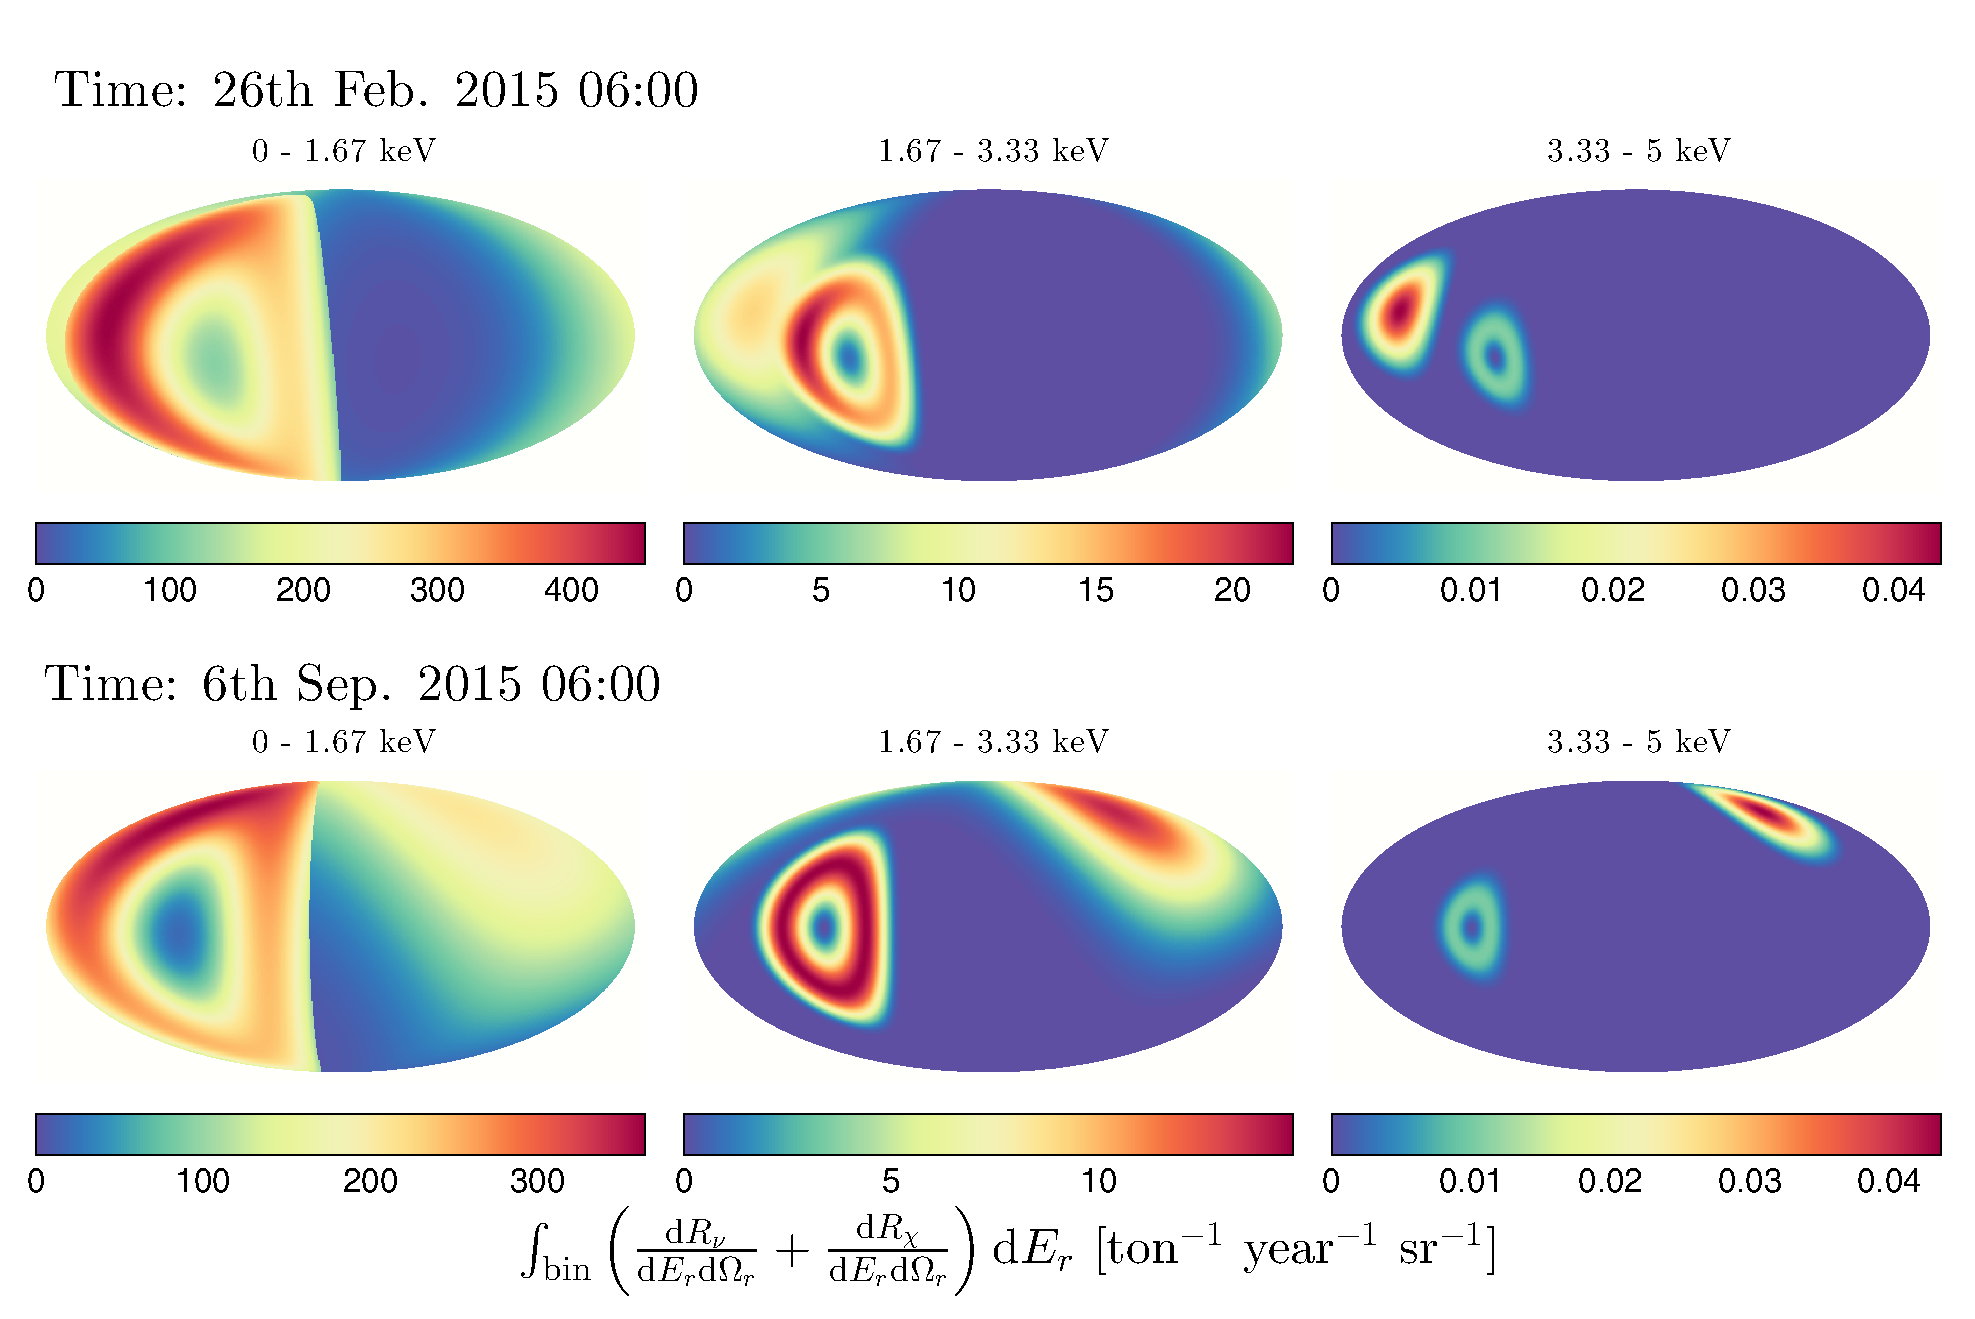
\includegraphics[trim = 0mm 0mm 0mm 0mm, clip, width=\textwidth,angle=0]{Figures/mollweide_minmax_times.eps}
\caption[Mollweide projections of the WIMP and $^8$B neutrino event rates]{Mollweide projections of the WIMP and $^8$B neutrino angular differential event rate ($R_\chi$ and $R_\nu$ respectively) integrated within (from left to right) three equally sized energy bins spanning the range $E_{r} = 0 \,$ to $5 \, {\rm keV}$, for a WIMP with mass $m_{\chi} = 6 \, {\rm GeV}$ and $\sigma^{\rm SI}_p = 5 \times 10^{-45} \, {\rm cm}^2$ and a ${\rm Xe}$ target.
The top row shows the signal on February 26th, when the separation between the directions of the Sun and Cygnus is smallest ($\sim 60^{\circ}$), and the bottom row on September 6th, when the separation is largest ($\sim 120^{\circ}$). The WIMP contribution is to the left of the neutrino contribution on the top row and to the right on the bottom row. The Mollweide projections are of the event rate in the laboratory coordinate system with the horizon aligned horizontally and the zenith and nadir at the top and bottom of the projection respectively.} 
\label{fig:Moll}
\end{center}
\end{figure}
Figure~\ref{fig:Moll} shows Mollweide projections of the laboratory frame angular differential event rate from a 6 GeV WIMP plus $^8$B Solar neutrinos,  at the times when the separation between the directions of the Sun and Cygnus are smallest and largest. Even at the time of smallest separation, the WIMP and neutrino recoil distributions can be easily distinguished as long as the angular resolution is better than a few tens of degrees. Although we only show the rates for $^8$B neutrino induced recoils, the angular distributions for other Solar neutrinos are very similar as neutrinos can only induce a recoil with an angle in the range $(0,\pi/2)$ from their incident direction. Additionally, the angular dependence of the recoil spectra is correlated with energy as can be seen going from the left to the right hand panels. For both the WIMP and neutrino recoils the angular spread decreases with increasing energy i.e. the highest energy recoils have the smallest angle between the incoming particle direction and the recoil direction.





\section{The neutrino floor}\label{sec:nufloor_nufloor}
\subsection{Discovery limits}
We now introduce the analysis methodology and the calculation of the neutrino floor as a discovery limit to {\it non}-directional detection experiments. Discovery limits were first introduced in Ref.~\cite{Billard:2011zj} and are defined such that if the true WIMP model lies above the limit then a given experiment has a 90\% probability to achieve at least a 3$\sigma$ WIMP detection. As such they are analogous to exclusion limits made by a particular experiment in practice however they relate to predictions for the range of WIMP cross sections to which a hypothetical experiment will be sensitive. The neutrino floor is a theoretical limit which is found by computing a discovery limit for an experiment that has a neutrino background. We describe this procedure in full in Appendix~\ref{app:likelihood}.

To calculate the neutrino floor we adopt a binned likelihood with $N_\textrm{bins}=100$ to allow us to efficiently perform our analysis with large numbers of neutrino events. The likelihood is written as the product of the Poisson probability distribution function ($\mathscr{P}$) for each bin, multiplied by individual likelihood functions parameterising the uncertainties on each neutrino flux normalisation and each astrophysical parameter,
\begin{align}\label{eq:likelihood}
 \mathscr{L}(m_\chi,\sigma^{\rm SI}_p,\boldsymbol{\Phi},\boldsymbol{\Theta}) = \prod_{i=1}^{N_\textrm{bins}} \mathscr{P} \left(N_\textrm{obs}^i \bigg| N^i_\chi + \sum_{j=1}^{n_\nu} N^{i}_\nu(\phi^j)\right) 
\prod_{j=1}^{n_\nu} \mathcal{L}(\Phi^j)
\prod_{k=1}^{n_\theta} \mathcal{L}(\theta^k) \, .
\end{align}
Where $\boldsymbol{\Phi} = \{ \Phi^1, ..., \Phi^{n_\nu} \}$ are the neutrino fluxes for each of the $n_\nu$ neutrino types and $\boldsymbol{\Theta} = \{\theta^1, ..., \theta^{n_\theta} \}$ contains the $n_\theta$ astrophysical uncertainties under consideration which will vary depending on the choice of velocity distribution e.g. the standard halo model: $\boldsymbol{\Theta}_\textrm{SHM} = \{ v_0,\vesc,\rho_0 \}$. The functions $\mathcal{L}(\phi^j)$ are the Gaussian parameterisations for each neutrino flux (see Table~\ref{tab:neutrino}) and similarly the likelihood functions $\mathcal{L}(\theta^k)$ parametrise the systematic uncertainty on each astrophysical parameter. Inside the Poisson function we have for each bin $i$, the observed number of events $N_\textrm{obs}^i$, the expected number of WIMP events $N_\chi^i$ given by,
\begin{equation}\label{eq:nchi}
N_\chi^i(m_\chi,\sigma^{\rm SI}_p,\boldsymbol{\Theta}) =\mathcal{E}\int_{E_{i}}^{E_{i+1}} \frac{\textrm{d} R_\chi}{\textrm{d}E_r} \textrm{d}E_r \, ,
\end{equation}
and $N_\nu^i(\phi^j)$ which is the expected number of neutrino events from the $j$th neutrino species,
\begin{equation}
N^{i}_\nu (\phi^j) = \mathcal{E}\int_{E_{i}}^{E_{i+1}} \frac{\textrm{d} R_\nu}{\textrm{d}E_r}(\phi^j) \textrm{d}E_r \, ,
\end{equation}
where $\mathcal{E}$ is the exposure of the experiment which we will quote in units of ton-year. We clarify here that the neutrino floor is not usually defined with the inclusion of any extra discrimination with timing information hence the likelihood is calculated assuming rates for WIMP and neutrinos that are constant in time. We adopt this convention to allow our neutrino floor limits to be compared with the literature. We show explicitly the added discrimination power brought by timing information in Sec.~\ref{sec:nufloor_time}.

\begin{figure}
\begin{center}
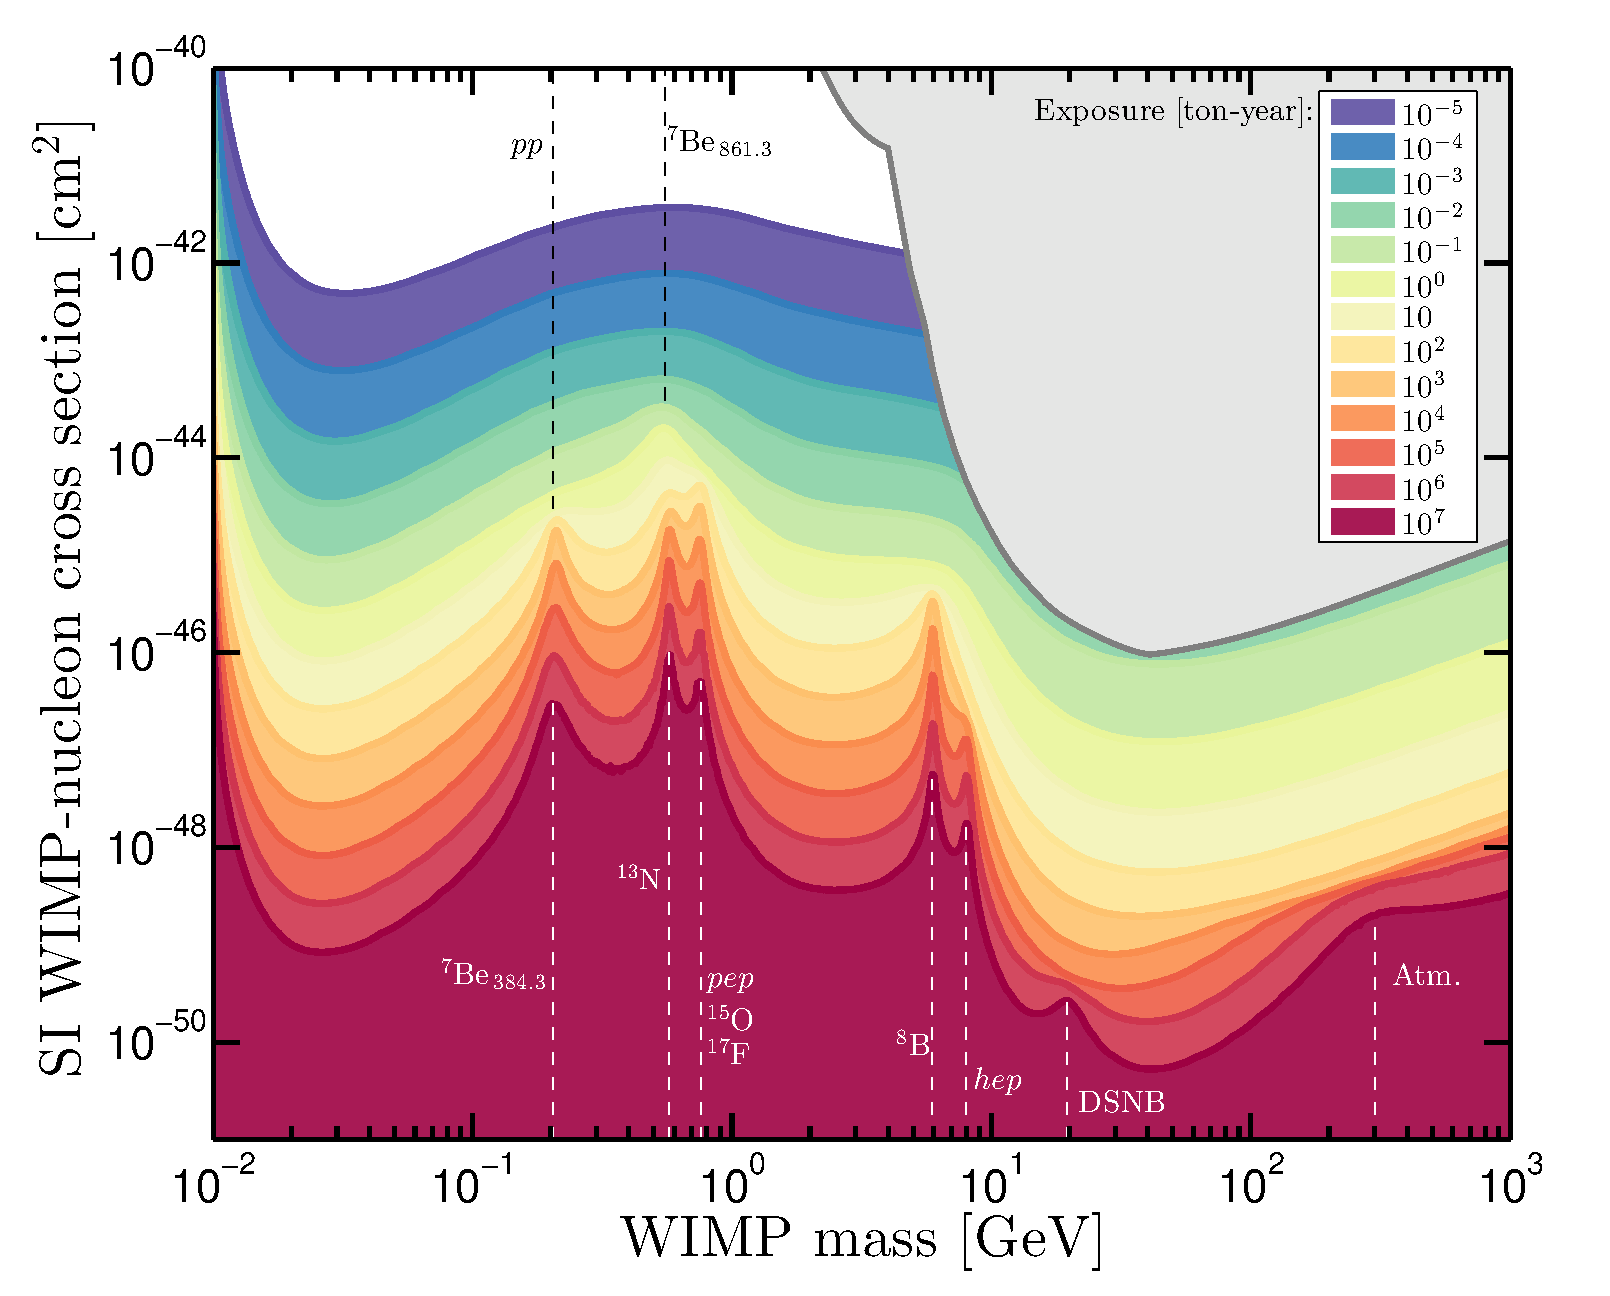
\includegraphics[trim = 0mm 0 0mm 0mm, clip, width=0.9\textwidth,angle=0]{Figures/EL_vs_mass_allNeutrinos.eps}
\caption[The complete SI xenon neutrino floor]{Illustration of the full dependence of the SI neutrino floor for a xenon target as a function of WIMP mass and detector exposure, showing the contribution from all sources of neutrino. The neutrino floor has peaks at WIMP masses where the xenon scattering rate for WIMPs and a certain neutrino source overlap. We indicate the region of this parameter space already excluded by experiments in grey.}
\label{fig:EL_vs_mass_allNeutrinos}
\end{center}
\end{figure} 
Figure~\ref{fig:EL_vs_mass_allNeutrinos} shows the full evolution of the discovery limit for a xenon experiment with an extremely low threshold (0.01 eV) to capture the neutrino floor down to $pp$ neutrino energies for completeness. It is important to note however that this Figure is merely an illustrative demonstration of each neutrino contribution as exposures of up to $10^7$ ton-years are clearly unfeasible. In Fig.~\ref{fig:EL_vs_mass_allNeutrinos} we see that the floor moves to lower cross sections as the exposure is increased as one would expect, however it acquires peaks where the WIMP recoil spectrum is mimicked by a given neutrino component. The mass at which a peak appears is dependent on the recoil energy range of the neutrino type. The cross section of the peak and how long the peak remains as exposure is increased depends on the uncertainty on the neutrino flux as well as how well the WIMP recoil event rate is mimicked by the neutrino type~\cite{Ruppin:2014bra}. With a smaller uncertainty it takes fewer WIMP events to distinguish them from neutrinos. The most important contribution to the neutrino floor is due to $^8$B neutrinos which cause a peak to appear at 6 GeV and are within the scope of upcoming direct detection experiments. There are also contributions from $hep$, atmospheric and DSNB neutrinos at higher WIMP masses which may be accessible in very large ($>100$ ton-year) experiments such as DARWIN~\cite{Aalbers:2016jon}. Finally, for low WIMP mass searches (below 1 GeV) there is a cluster of peaks due to the lower energy Solar neutrinos: $pp$, $pep$, $^7$Be, $^{15}$O, $^{13}$N and $^{14}$F.

As we displayed with Fig.~\ref{fig:WIMPlimits_SI} in Chapter~\ref{chapter:direct}, the neutrino floor also depends upon the target nucleus and whether one considers SI or SD interactions. For clarity in describing the phenomenology of the neutrino floor we show just limits for a xenon target experiment. In the SI independent case the limits are extremely similar for different mass targets however one must take care translating between different nuclear enhancement factors and isotopic fractions in the SD case. Differences in these factors give rise to large shifts in cross section between the floors for various spin-possessing targets. Exploiting target complementarity is therefore a much more useful strategy for mitigating the SD neutrino floor~\cite{Ruppin:2014bra}. 

\subsection{Neutrino flux uncertainties}\label{sec:nufloor_nufluxunc}
\begin{figure}
\begin{center}
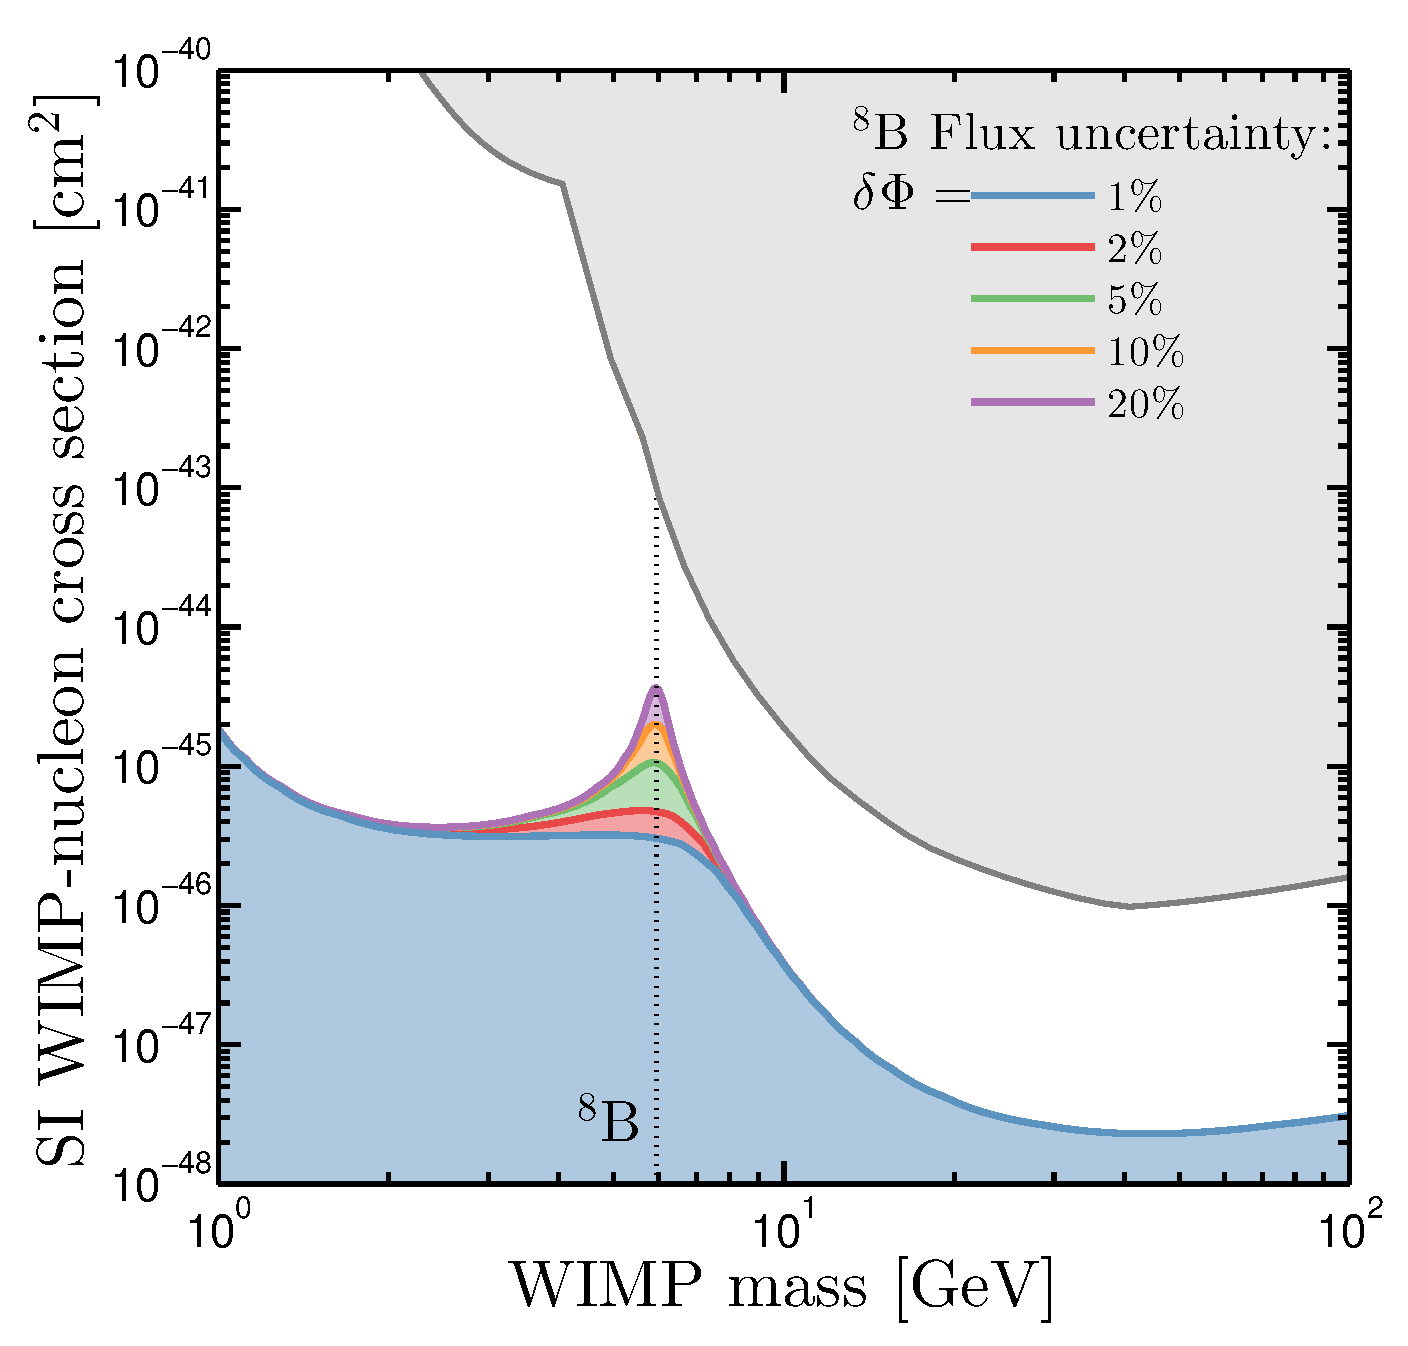
\includegraphics[trim = 0mm 0 0mm 0mm, clip, width=0.48\textwidth,angle=0]{Figures/nufloor_fluxerrs.eps}
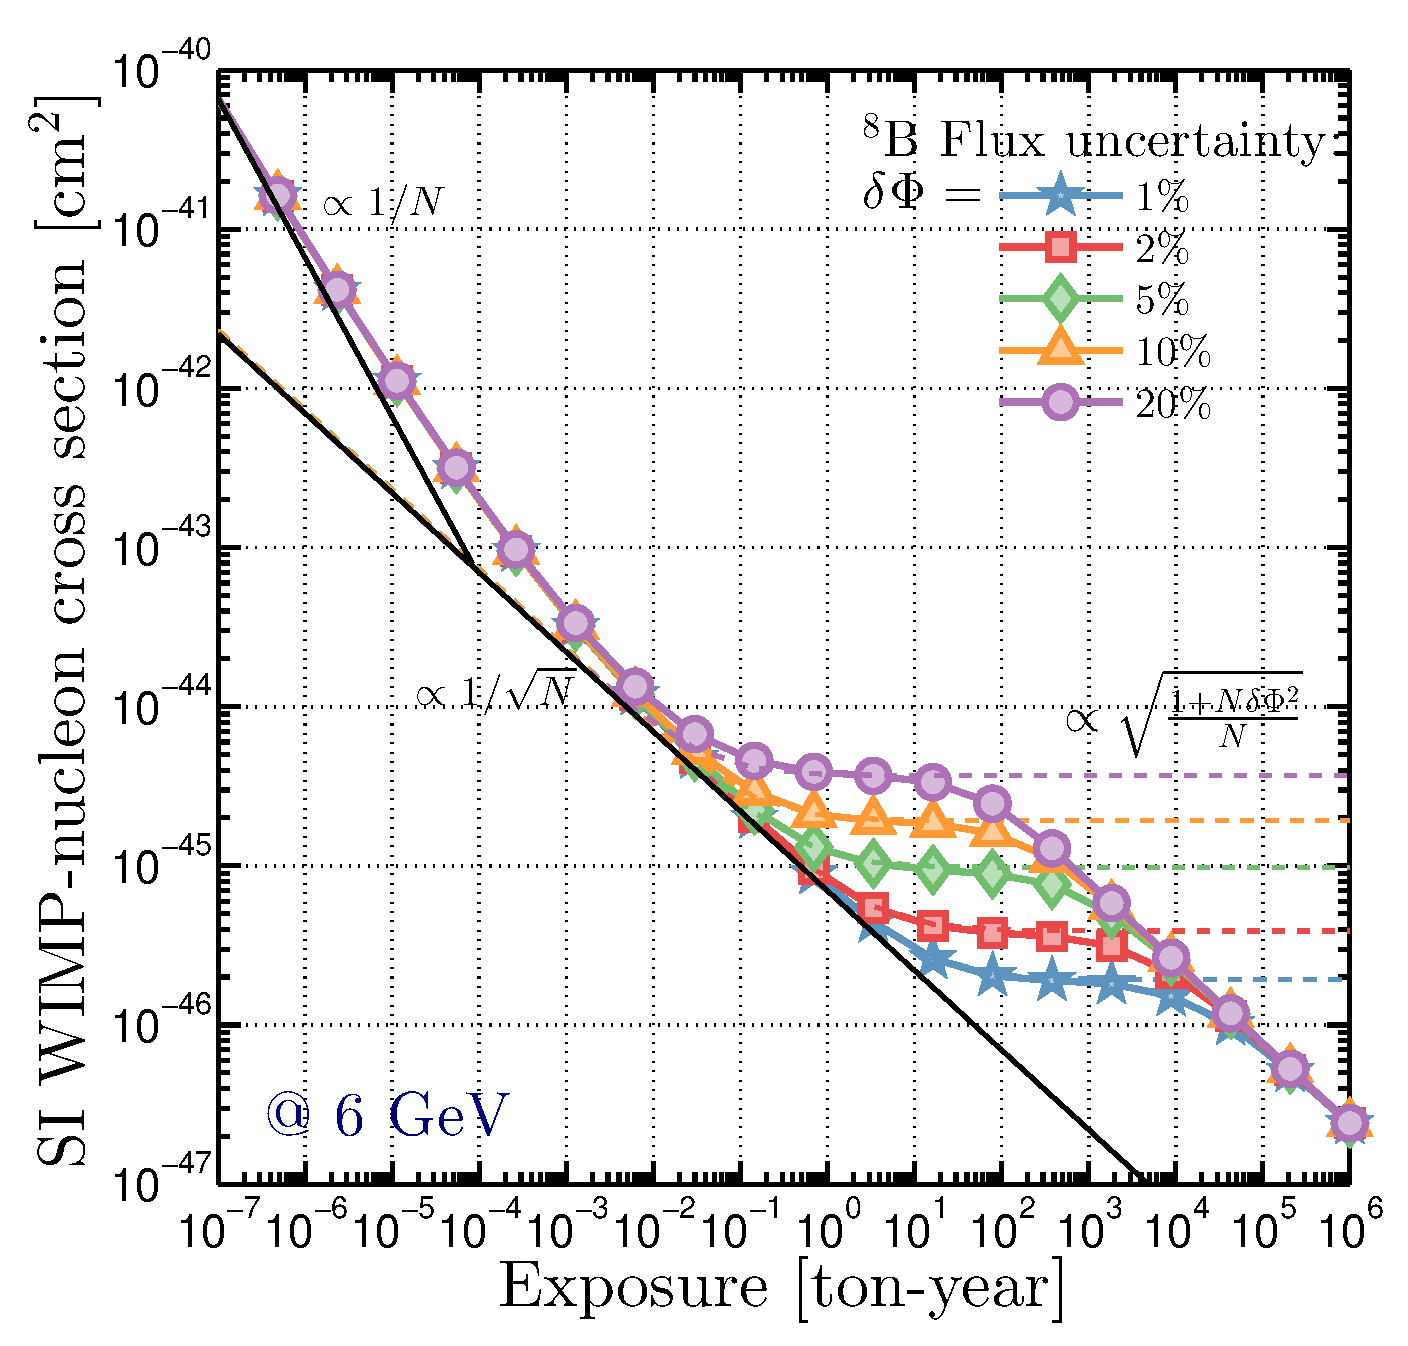
\includegraphics[trim = 0mm 0 0mm 0mm, clip, width=0.48\textwidth,angle=0]{Figures/nufloor_fluxerrsex.eps}
\caption[Effect of the flux uncertainty on the neutrino floor]{SI xenon neutrino floor as a function the uncertainty on the $^8$B neutrino flux. {\bf Left}: the neutrino floor for a 10 ton-year xenon experiment as a function of WIMP mass for flux uncertainties in the range 1\%~-~20\%. We also show the region currently excluded by experiments in grey. {\bf Right}: the evolution of the neutrino floor {\it at} 6 GeV as a function of detector exposure for the same range of flux uncertainty values. We also indicate the three scaling regimes with number of background events $N$.}
\label{fig:nufluxunc}
\end{center}
\end{figure} 
The shape of the neutrino floor (and in fact the presence of the limit itself) is controlled by the level of uncertainty in the expected CNS signal. In the left hand panel of Fig.~\ref{fig:nufluxunc} we show how the assumption for the uncertainty on the $^8$B flux affects the height of the neutrino floor in cross section: for lower uncertainties the neutrino floor appears at lower cross sections, even though the average number of $^8$B events observed in each case is the same. In the right hand panel we show an alternative perspective on the same phenomenon, displaying instead the evolution of the value of the discovery limit at 6 GeV as the exposure of the experiment increases. 

The limits in the right-hand panel of Fig.~\ref{fig:nufluxunc} can be seen evolving through three regimes that we express in terms of the number of background events, $N$. Initially, towards very low exposures the limit approaches a $1/N$ scaling; this is the case for experiments that have less than 1 expected background event over the exposure time. Then as the exposure increases, the limit transitions into a standard Poisson background subtraction regime, scaling as $1/\sqrt{N}$. In experiments with measures to try and distinguish signal from background events, the discovery limit would proceed as $N$ increases in much the same way. However in the presence of neutrinos which mimic the signal, the discovery limit plateaus. The evolution of the discovery limit in this regime is controlled by the systematic uncertainty on the dominant neutrino component according to~\cite{Billard:2013qya},
\be
\sigma_{\rm DL} \propto \sqrt{\frac{1+N\delta \Phi^2}{N}},
\ee
where $\sigma_{\rm DL}$ is the discovery limit and $\delta \Phi$ is the fractional uncertainty on the relevant neutrino flux. In this regime, which persists for $N~\sim 10-1000$, the experiment cannot tell the difference between WIMP and neutrino induced recoils. This saturation of the WIMP sensitivity, spanning over two orders of magnitude in exposure, is what is commonly referred to as the neutrino floor. With statistics at this level the experiment cannot probe WIMP cross sections that induce excesses in the total number of observed events smaller than what could just be attributed to fluctuations within the allowed background uncertainty. For instance, one could imagine a hypothetical situation in which the expected neutrino event rate was known with perfect certainty, in this case there would be no limit to how small a cross section an experiment could probe because, up to Poisson fluctuations, one would know how many events one would need to attribute to neutrino recoils. Unfortunately, in reality we have a finite uncertainty and this will lead to a saturation of any WIMP signal as more neutrino events are seen. It should be noted however that this scaling regime does not continue indefinitely. Eventually the slight differences in the tails of the neutrino and WIMP event rates allow the two spectra to be distinguished once a sufficient number of events have been detected, usually around $\mathcal{O}(1000)$~\cite{Ruppin:2014bra}. Although as can be seen in Fig.~\ref{fig:nufluxunc}, the exposures needed depend on the flux uncertainty.

It is important to keep these uncertainties in mind when projecting future limits because neutrino experiments and Solar model builders are also trying to independently reduce them. For this reason it is likely that the neutrino floor problem will be alleviated somewhat over time as better estimates are made, without any further effort on the part of direct detection experiments. Importantly though this is not a permanent solution, the neutrino floor in this scenario is simply suppressed to lower cross sections. For the remainder of our results we will fix to the current best estimates to the neutrino flux uncertainties as we have already described.

\subsection{Astrophysical uncertainties}\label{sec:nufloor_astro}
\begin{figure}
\begin{center}
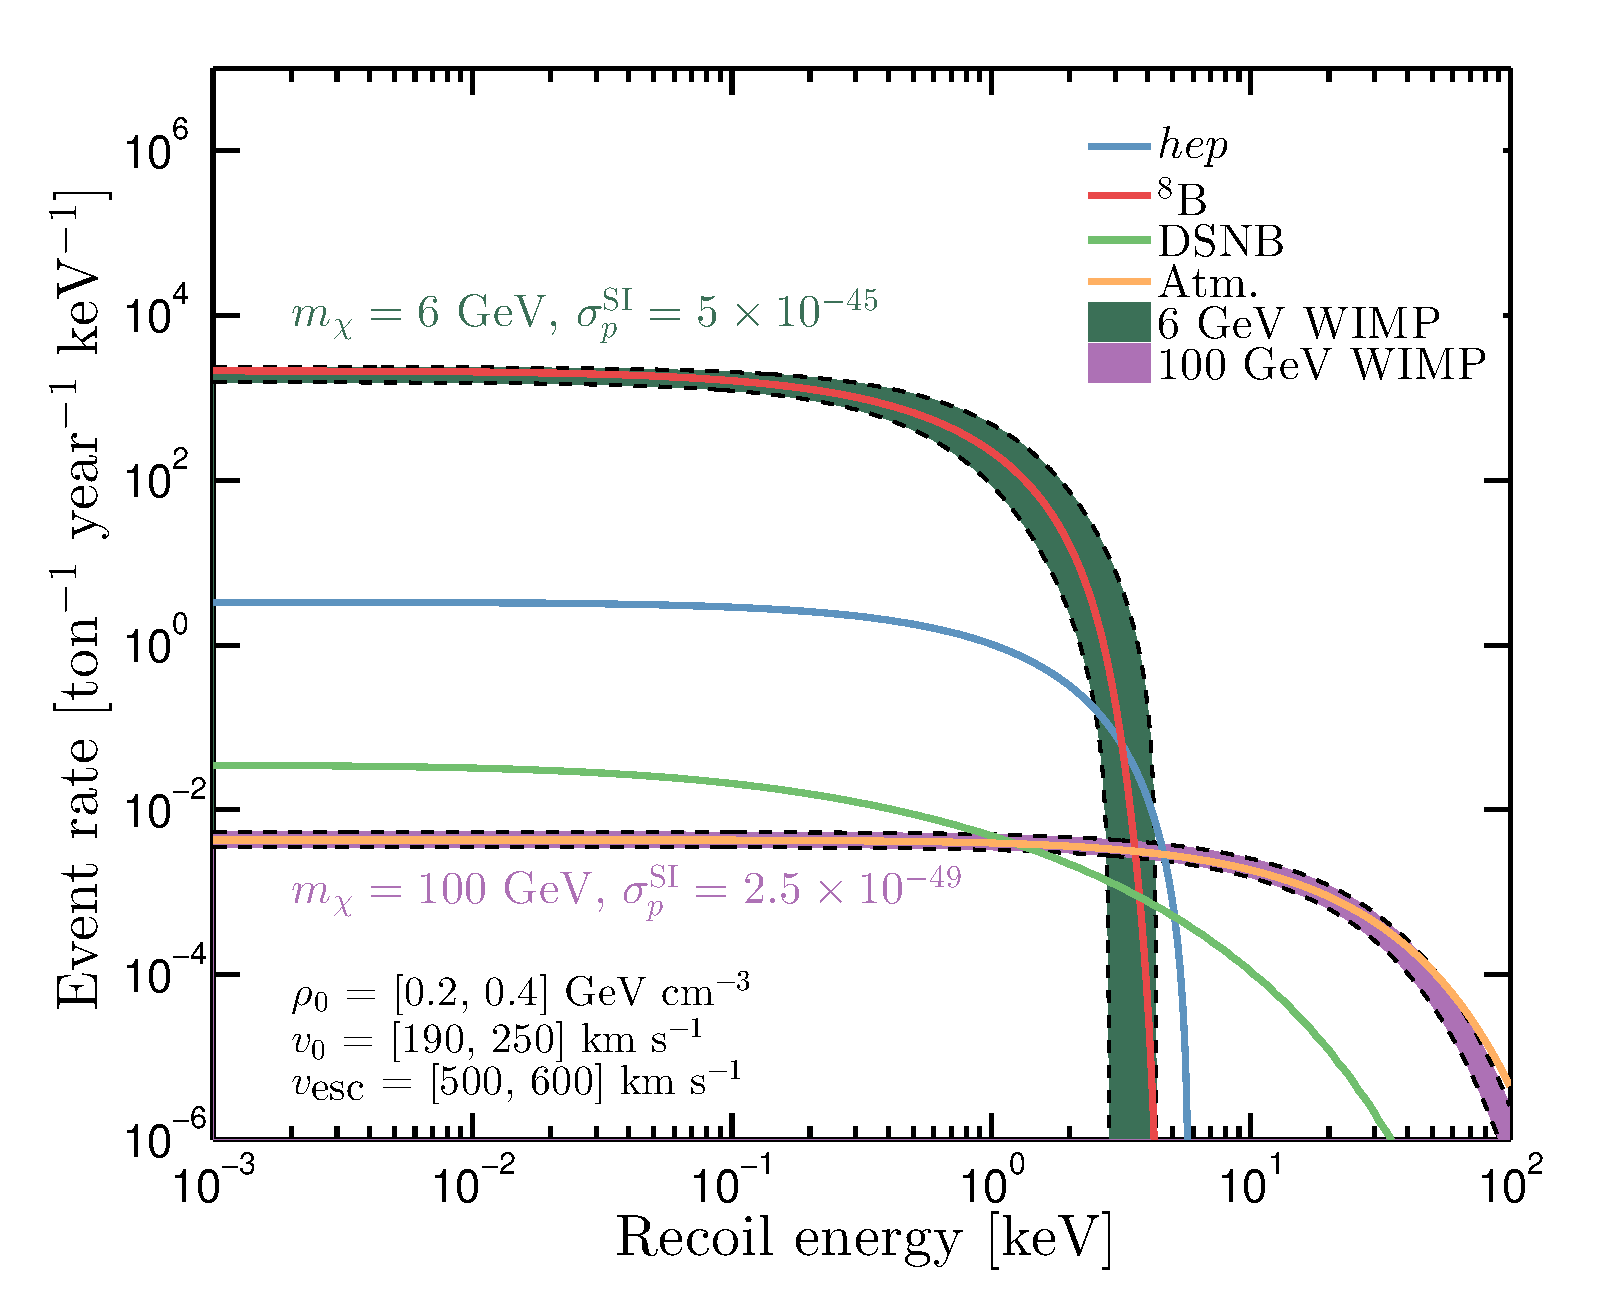
\includegraphics[trim = 0mm 0 0mm 0mm, clip, width=0.8\textwidth,angle=0]{Figures/EventRates_with_uncertainties.eps}
\caption[Effect of astrophysical uncertainties on WIMP recoil spectra]{SI xenon elastic scattering rates for 6 and 100 GeV WIMPs and 4 neutrino sources ($hep$, $^8$B, DSNB and atmospheric neutrinos). The dark green and orange shaded regions respectively refer to the range of scattering rates for 6 and 100 GeV WIMPs with standard halo model parameters taking values between $\rho_0 = [0.2,0.4]$~GeV~cm$^{-3}$, $v_0 = [190,250]$~km~s$^{-1}$ and $\vesc = [500,600]$~km~s$^{-1}$.}
\label{fig:EventRates_with_uncertainties}
\end{center}
\end{figure} 
In addition to sources of uncertainty from the neutrino input we must also consider uncertainties in the WIMP input. We now explain how astrophysical uncertainties influence the shape of the neutrino floor. We focus here on the low mass region. Because light WIMPs probe the tail of the speed distribution, limits in this regime have a greater sensitivity to the values of astrophysical parameters. This choice is also motivated by the fact that advances in technology are more likely to bring about lower threshold detectors (giving access to these low WIMP masses)~\cite{Mirabolfathi:2015pha,Kadribasic:2017obi} than allow exposures in excess of $10^3$ ton-years to be achieved (which are required to reach the neutrino floor due to atmospheric and diffuse supernovae neutrinos).

Figure~\ref{fig:EventRates_with_uncertainties} shows the energy dependence of the nuclear recoil event rate over a range of input values for three free parameters: local density $\rho_0$, circular rotation speed $v_0$ and escape velocity $\vesc$. As mentioned in Sec~\ref{sec:nufloor_nufloor} we see that light WIMPs have a greater sensitivity to changes in the astrophysical input than heavier WIMPs and that the most visible change is around the tail of the recoil distribution (around 1 keV for a 6 GeV WIMP for example). We first discuss the effect of each parameter individually, before embedding the uncertainties in the calculation of the neutrino floor itself.

\begin{figure}
\begin{center}
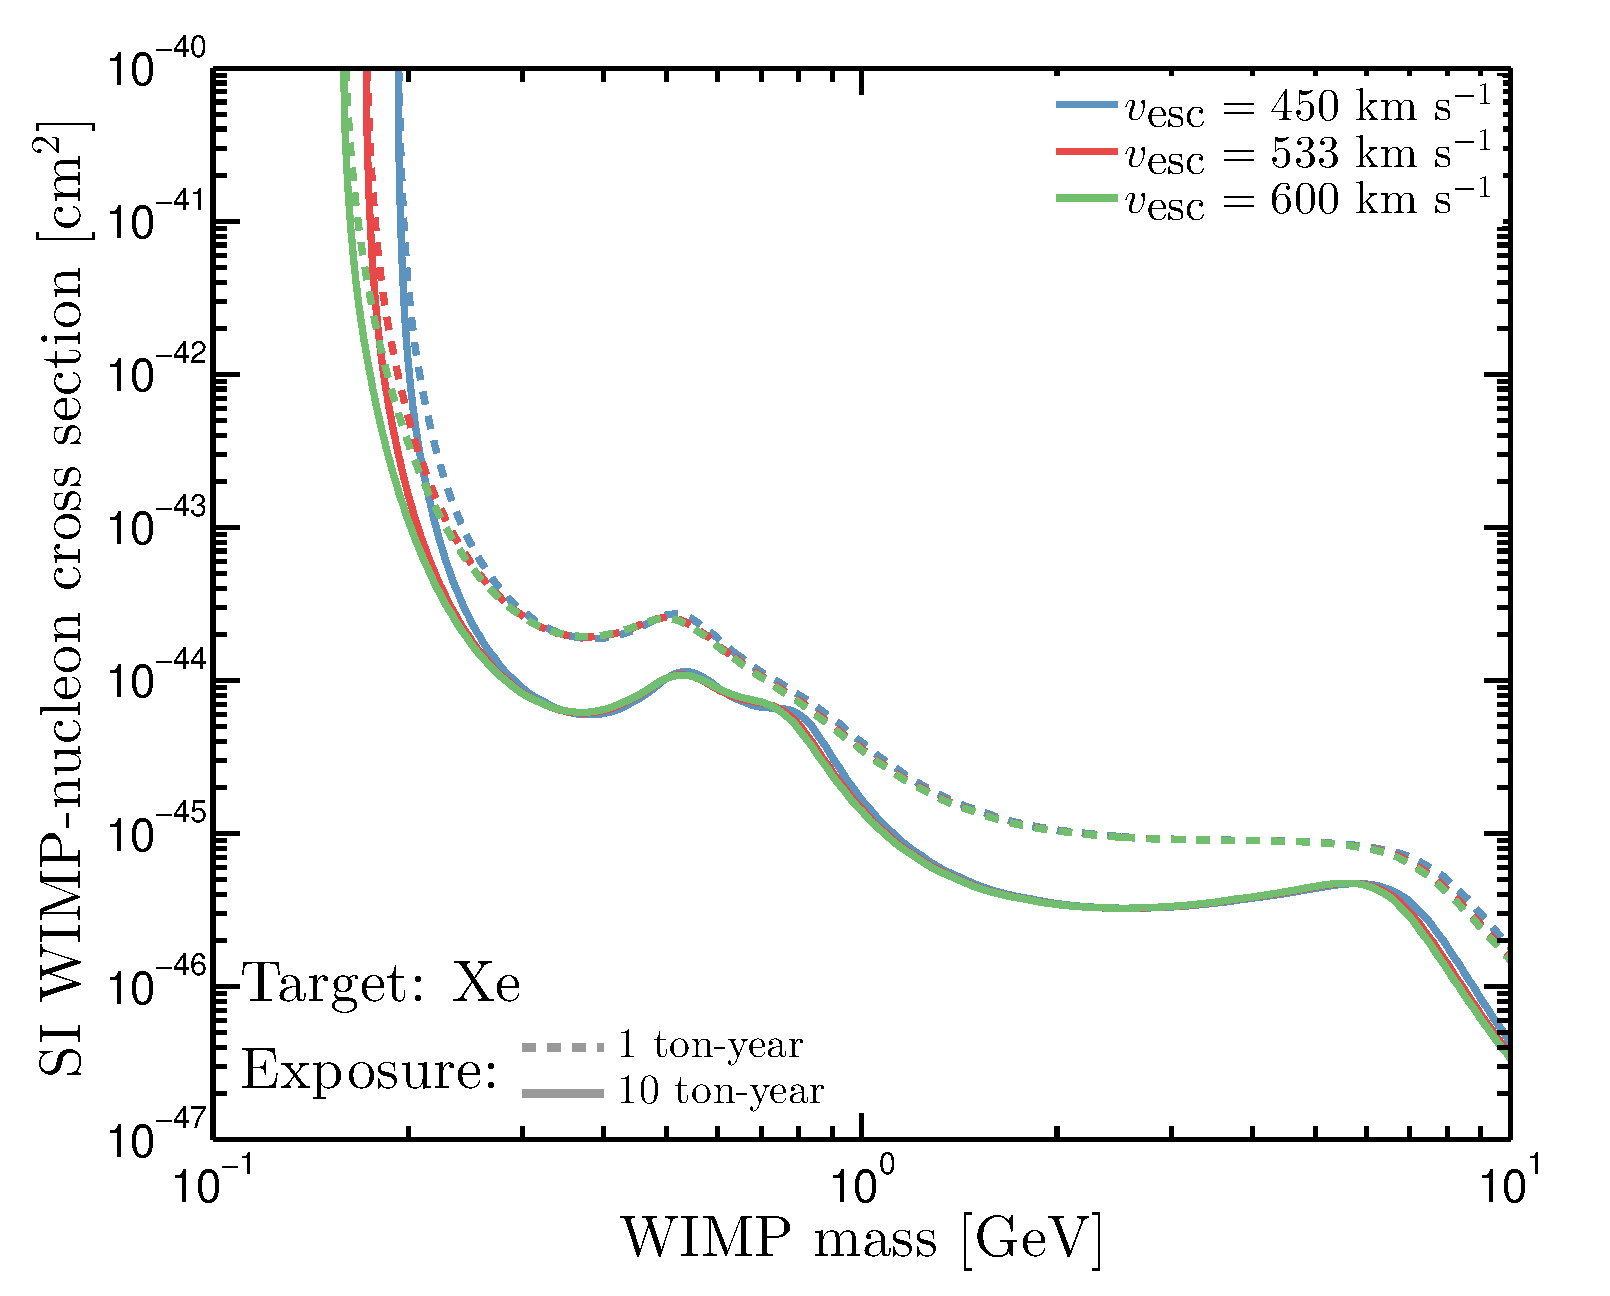
\includegraphics[trim = 0mm 0 0mm 0mm, clip, width=0.8\textwidth,angle=0]{Figures/DL_vesc.eps}
\caption[Neutrino floor with different values of input escape velocity]{SI neutrino floor for a xenon experiment with different values of input escape velocity. The dashed lines are for a 1 ton-year exposure and the solid lines for a 10 ton-year exposure. The blue, red and green colours correspond to input escape velocities of 450, 533 and 600~km~s$^{-1}$ respectively.}
\label{fig:DL_vesc}
\end{center}
\end{figure} 
{\bf The escape velocity} in principle sets the maximum WIMP speed that can be detected on Earth. Since the escape velocity can only control the tail of the recoil distribution and because the speed distribution is very small at its tail, the effect of changing the speed at which it is truncated only has a small impact on the overall shape of the recoil energy spectrum. Figure~\ref{fig:DL_vesc} shows the neutrino floor for 3 values of the escape velocity demonstrating only very marginal differences in the overall shape. The most noticeable effect is around 0.2 GeV where the limits sharply increase due to the maximum energy recoils falling below 3 eV. This is not strictly a feature of the neutrino floor but an artifact of the calculation being performed with a finite cutoff. Apart from some very slight differences in the floors around 0.8 GeV and 8 GeV they are largely indistinguishable. It should be noted that the values of escape velocity chosen in Fig.~\ref{fig:DL_vesc} cover a wider range than the quoted systematic uncertainty in the observed RAVE value of 533 km s$^{-1}$~\cite{Piffl:2013mla}. We deduce that including the uncertainty on $\vesc$ will only have a small effect.




\begin{figure}
\begin{center}
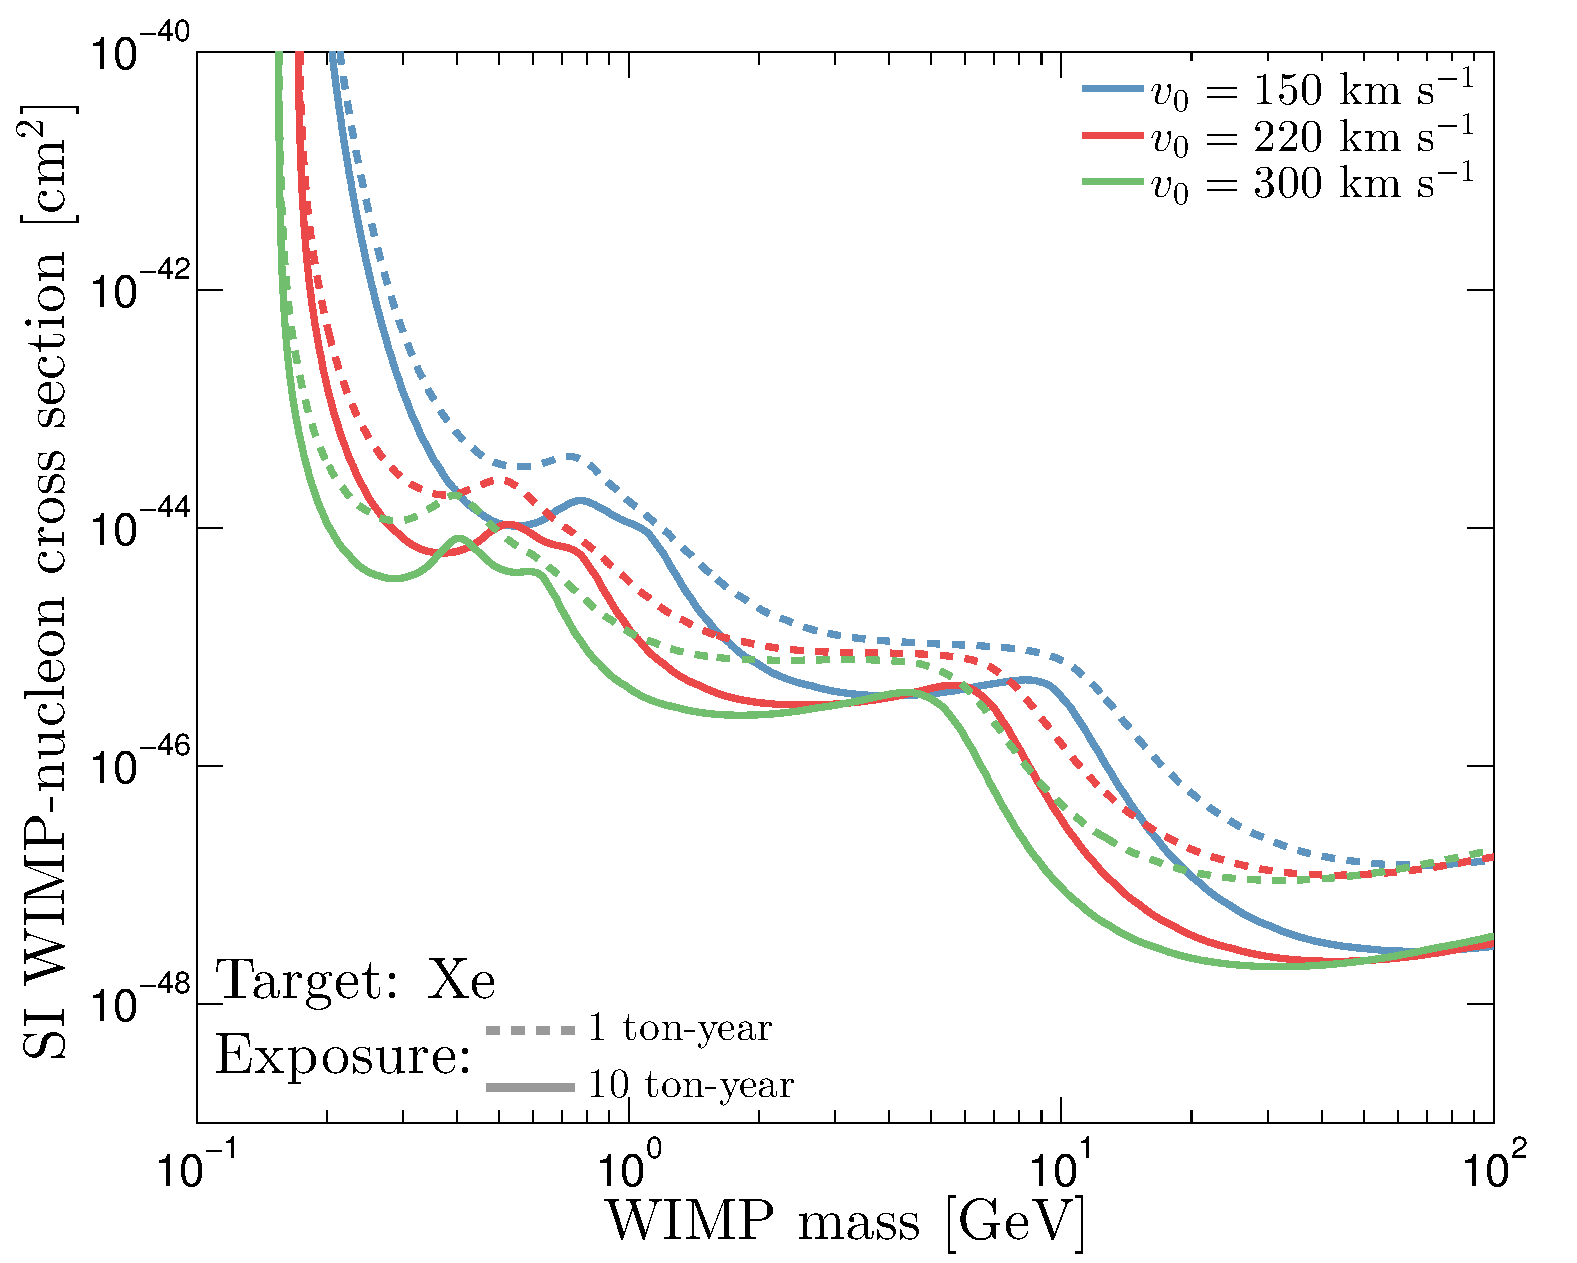
\includegraphics[trim = 0mm 0 0mm 0mm, clip, width=0.8\textwidth,angle=0]{Figures/DL_v0-eps-converted-to.pdf}
\caption[Neutrino floor with different values of input circular velocity $v_0$]{SI neutrino floor for a xenon experiment with different values of input circular velocity $v_0$. The dashed lines are for a 1 ton-year exposure and the solid lines for a 10 ton-year exposure. The blue, red and green colours correspond to an input $v_0$ of 150, 220 and 300 km~s$^{-1}$ respectively.}
\label{fig:DL_v0}
\end{center}
\end{figure} 
{\bf Lab velocity}: The largest source of uncertainty in the laboratory velocity comes from the Sun's circular speed, $v_0$. Given the discrepancies between astronomically observed values for $v_0$, both with each other and with the fiducial value of 220~km~s$^{-1}$~\cite{McMillan:2009yr}, we will be pessimistic about our chosen uncertainty on $v_0$. Figure~\ref{fig:DL_v0} shows the neutrino floor for a range of values of $v_0$. Compared to Fig.~\ref{fig:DL_vesc}, the effect of $v_0$ is much more noticeable. Whereas $\vesc$ influences only the tail of the recoil energy distribution, $v_0$ influences the entirety. For smaller values of $v_0$, larger $m_\chi$ values become mimicked by the same neutrino type, hence the neutrino floor is shifted to higher masses and vice versa.
 
{\bf The local density} appears as a multiplicative factor in the WIMP event rate and as already discussed is degenerate with the scattering cross section. For this study the effect of changing local density is straightforward: a larger value of $\rho_0$ simply shifts the floor to smaller cross sections by the same factor.

\begin{figure}
\begin{center}
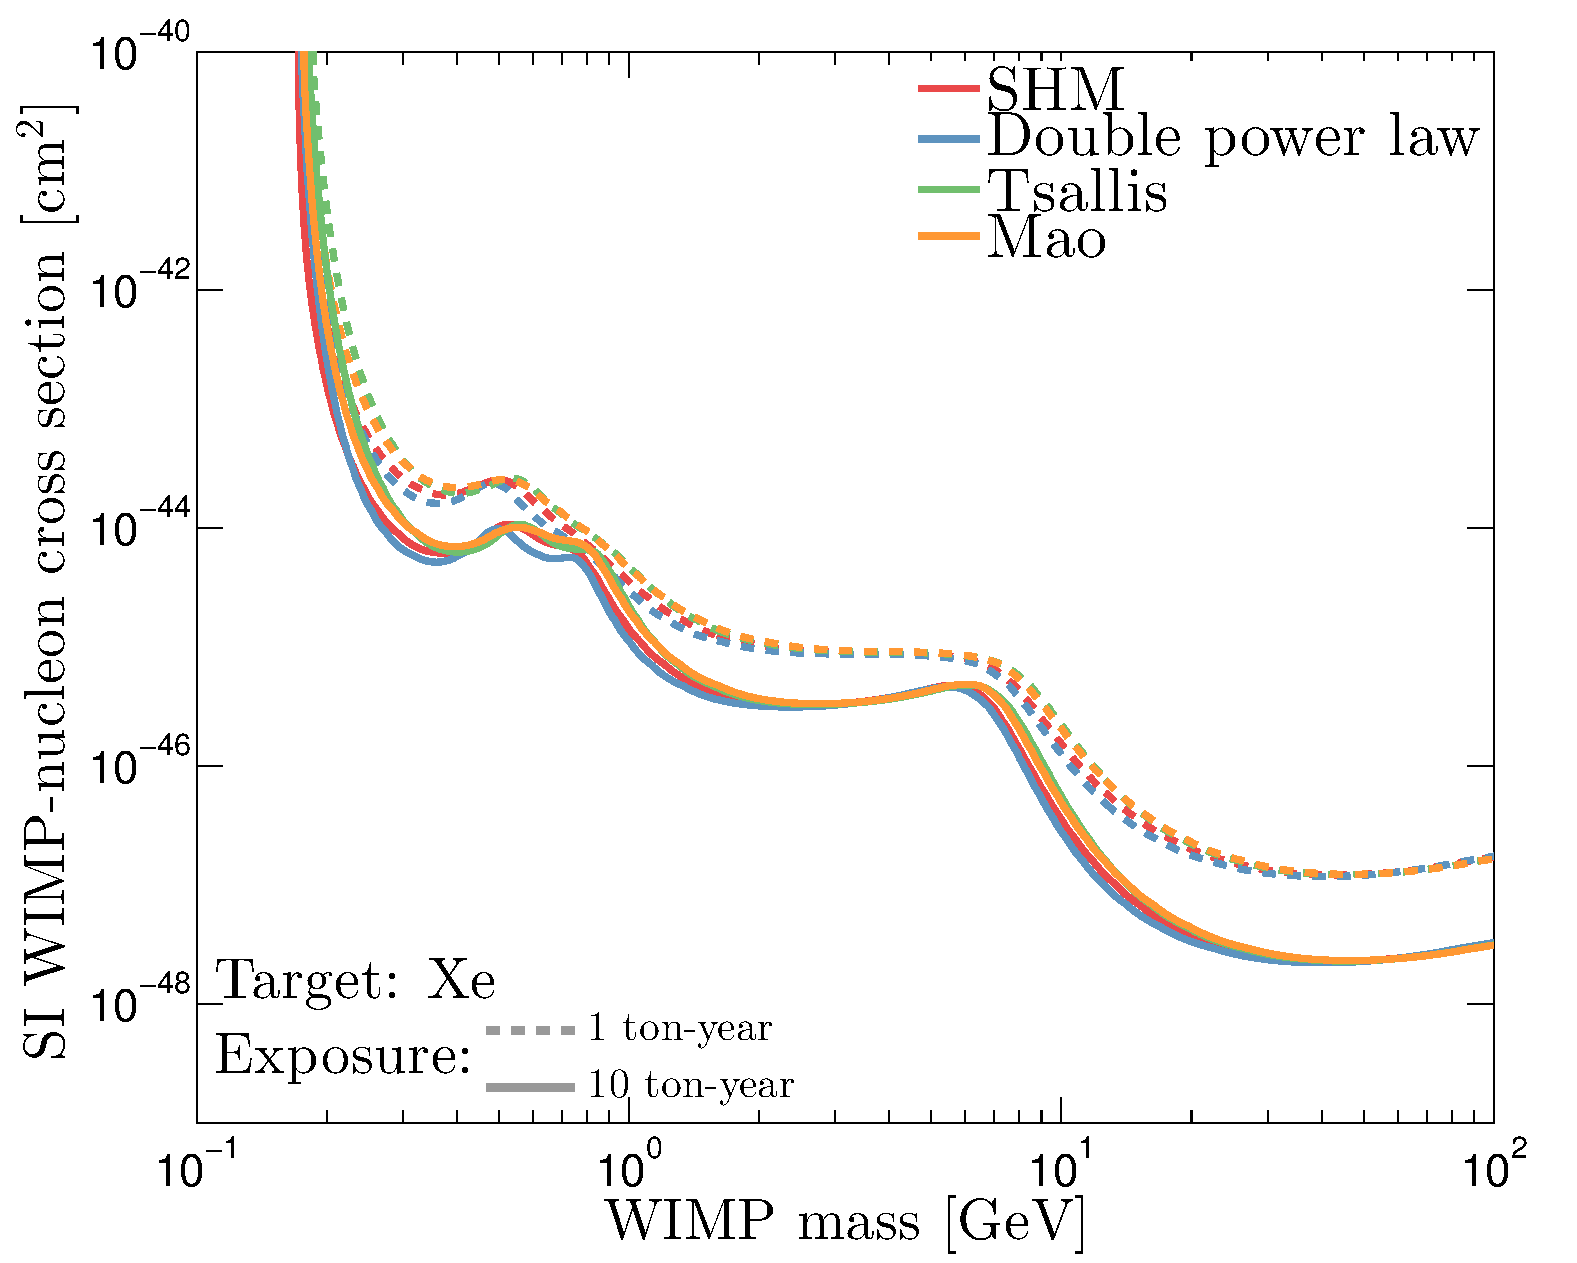
\includegraphics[trim = 0mm 0 0mm 0mm, clip, width=0.8\textwidth,angle=0]{Figures/DL_fv-eps-converted-to.pdf}
\caption[Neutrino floor with different input speed distributions]{SI neutrino floor for a xenon experiment for various input speed distributions. The dashed lines are for a 1 ton-year exposure and the solid lines for a 10 ton-year exposure. The blue, green and orange colours correspond to the double power law, Tsallis and Mao distributions respectively. The red lines are for the SHM with $v_0 = 220$~km~s$^{-1}$ and $v_\textrm{esc} = 533$~km~s$^{-1}$.}
\label{fig:DL_fv}
\end{center}
\end{figure} 
{\bf Speed distribution}: The neutrino floors for alternative speed distributions are shown in Fig.~\ref{fig:DL_fv}. These alternatives, the `double power law', `Tsallis' and `Mao' distributions are outlined in full in Appendix~\ref{app:fv}. They are notable for having departures from a Maxwellian shape at high speeds. For distinguishing neutrinos and WIMPs the high energy tail is important hence we expect that this may induce changes to the shape of the floor. However when we input different underlying speed distributions the position of the floor is altered only very slightly; shifting to slightly higher WIMP masses for the double power law and Mao models and to slightly smaller masses for the Tsallis model. For this reason, and in the interest of efficiency, from here we focus our attention on the SHM. 

\begin{figure}
\begin{center}
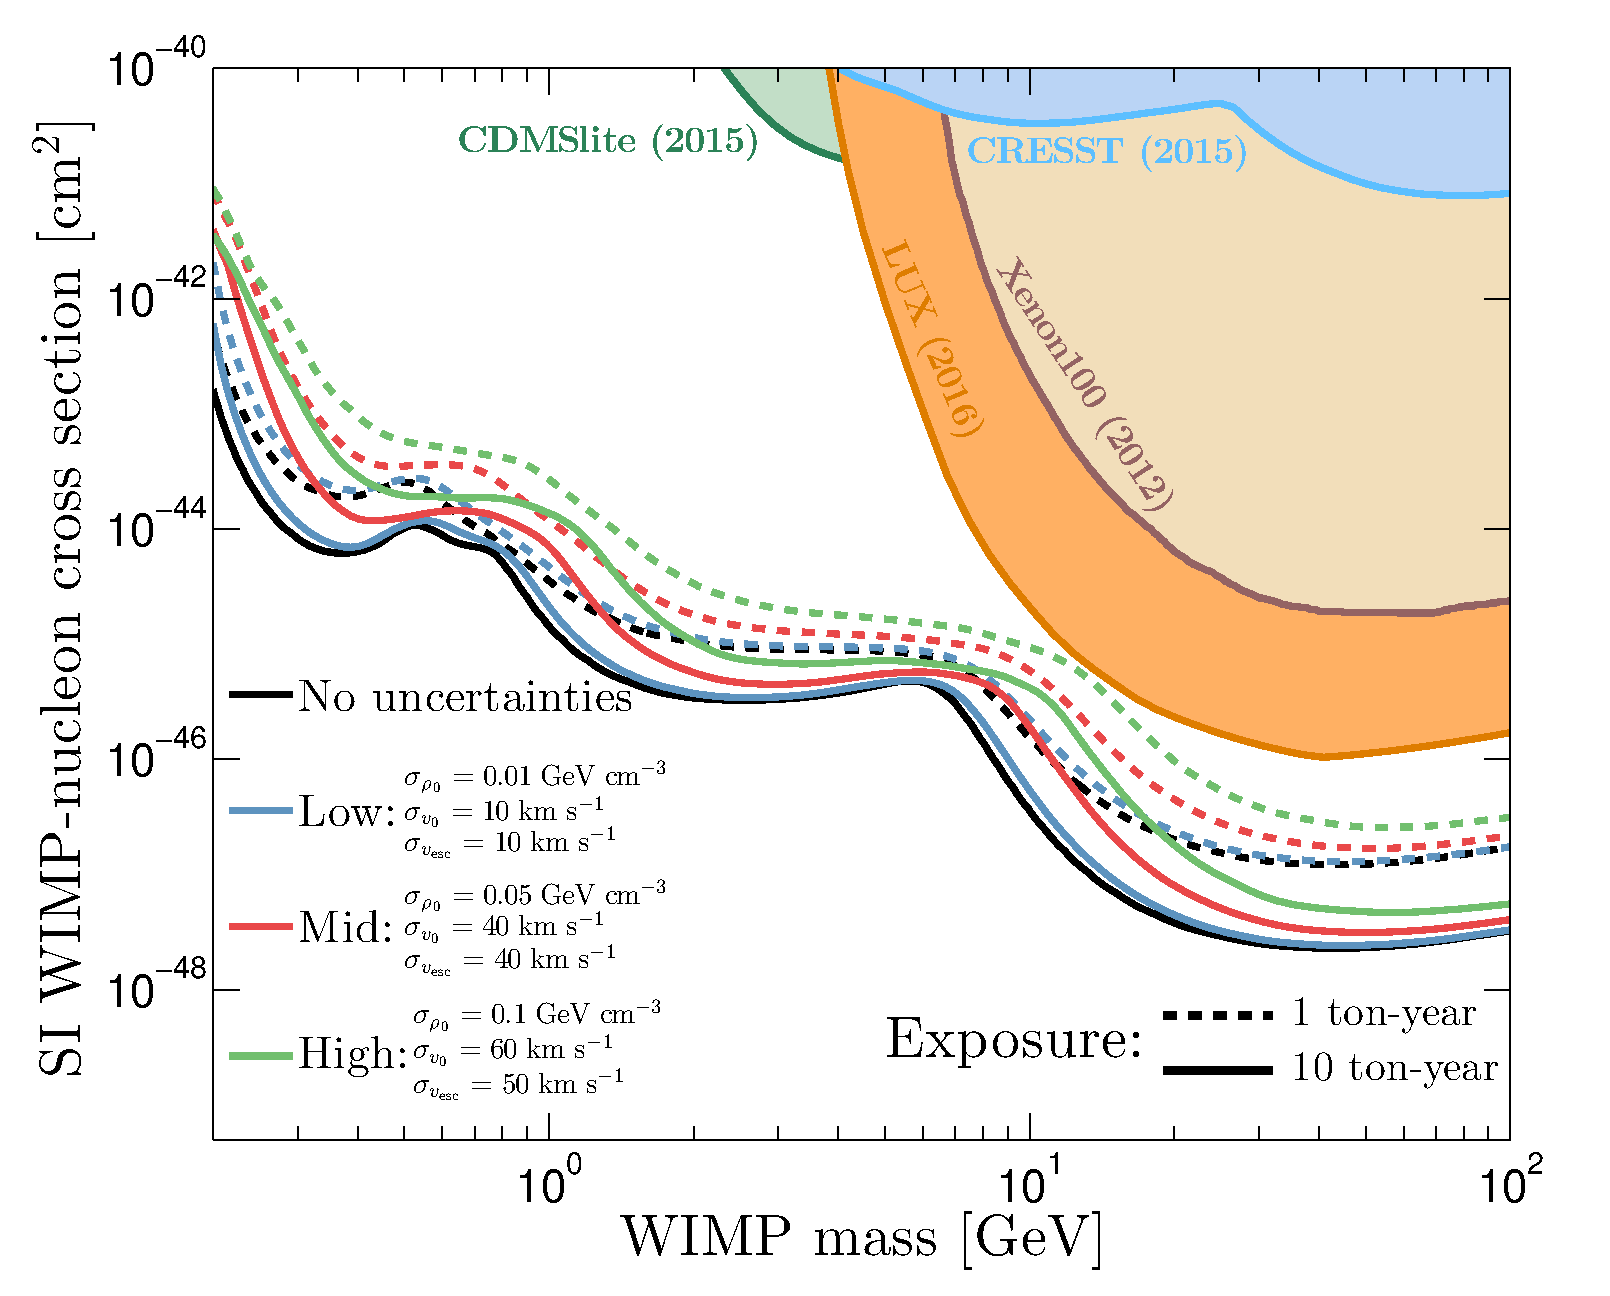
\includegraphics[trim = 0mm 0 0mm 0mm, clip, width=0.8\textwidth,angle=0]{Figures/DL_Uncertainties.eps}
\caption[Neutrino floor with the inclusion of astrophysical uncertainties]{SI neutrino floor as a function of WIMP mass calculated with the inclusion of astrophysical uncertainties in the profile likelihood ratio analysis. The dashed lines are for an exposure of 1 ton-year and the solid lines are with an exposure of 10 ton-years. The blue, red and green curves correspond to 3 sets of values of the 1$\sigma$ uncertainty on the parameters $\rho_0$, $v_0$ and $\vesc$ displayed on the Figure and in the text. The size of the uncertainties are labelled from low to high with values indicated. The filled regions are excluded by experiments, CRESST~\cite{Angloher:2015ewa}, CDMSlite~\cite{Agnese:2015nto}, Xenon100~\cite{Aprile:2012nq} and LUX~\cite{Akerib:2016vxi}.}
\label{fig:DL_uncertainties}
\end{center}
\end{figure}
Now that we have demonstrated the impact of each parameter individually, we unfix them in the profile likelihood ratio test and account for their uncertainty with a multiplicative Gaussian factor. Figure~\ref{fig:DL_uncertainties} shows the discovery limits as a function of the width of this Gaussian uncertainty. We label the sets of uncertainty values ``low'', ``mid'' and ``high''. The low values for the 1$\sigma$ uncertainty on $\rho_0$, $v_0$ and $\vesc$ are respectively, 0.01~GeV~cm$^{-3}$, 10~km~s$^{-1}$ and 10~km~s$^{-1}$. The mid values are 0.05~GeV~cm$^{-3}$, 40~km~s$^{-1}$ and 40~km~s$^{-1}$. And for the high values we use 0.1~GeV~cm$^{-3}$, 60~km~s$^{-1}$ and 50~km~s$^{-1}$.

With the values of the astrophysical parameters uncertain, the experiment is less powerful. The neutrino floor in these cases appears at larger cross sections because the WIMP signal is statistically saturated with fewer events. We also find that the maxima appearing in the discovery limit due to each neutrino component become broader with the inclusion of uncertainties. As shown in the previous Section, the peak in the discovery limit shifts to WIMP masses with recoil energies more closely matching that of the relevant neutrino. Hence, the larger the uncertainty on $v_0$ and $v_\textrm{esc}$ the broader the peak becomes due to the increased range of WIMP masses with recoil energies overlapping with neutrinos. For instance the peak due to $^8$B neutrinos now extends up to 15 GeV for the largest set of astrophysical uncertainties.

This result shows that it is important for the astrophysical input to the predicted WIMP event rate to be well understood if one wishes to interpret how neutrinos play a role in prohibiting the discoverability of certain regions of the WIMP mass-cross section parameter space. Particularly this will be a concern for the next generation of direct detection experiments which are set to make limits that come very close to those calculated in this work. In fact, as we can see in Fig.~\ref{fig:DL_uncertainties}, the floor for ``high'' values of uncertainty comes extremely close to the LUX limit just above 10 GeV. Hence we can conclude that unless there are improvements in the knowledge of the astrophysics parameters or the uncertainties on the neutrino flux, the neutrino floor will be encountered by direct detection experiments much sooner than previously thought.


\subsection{Future detectors}\label{sec:nufloor_future}
\begin{figure}
\begin{center}
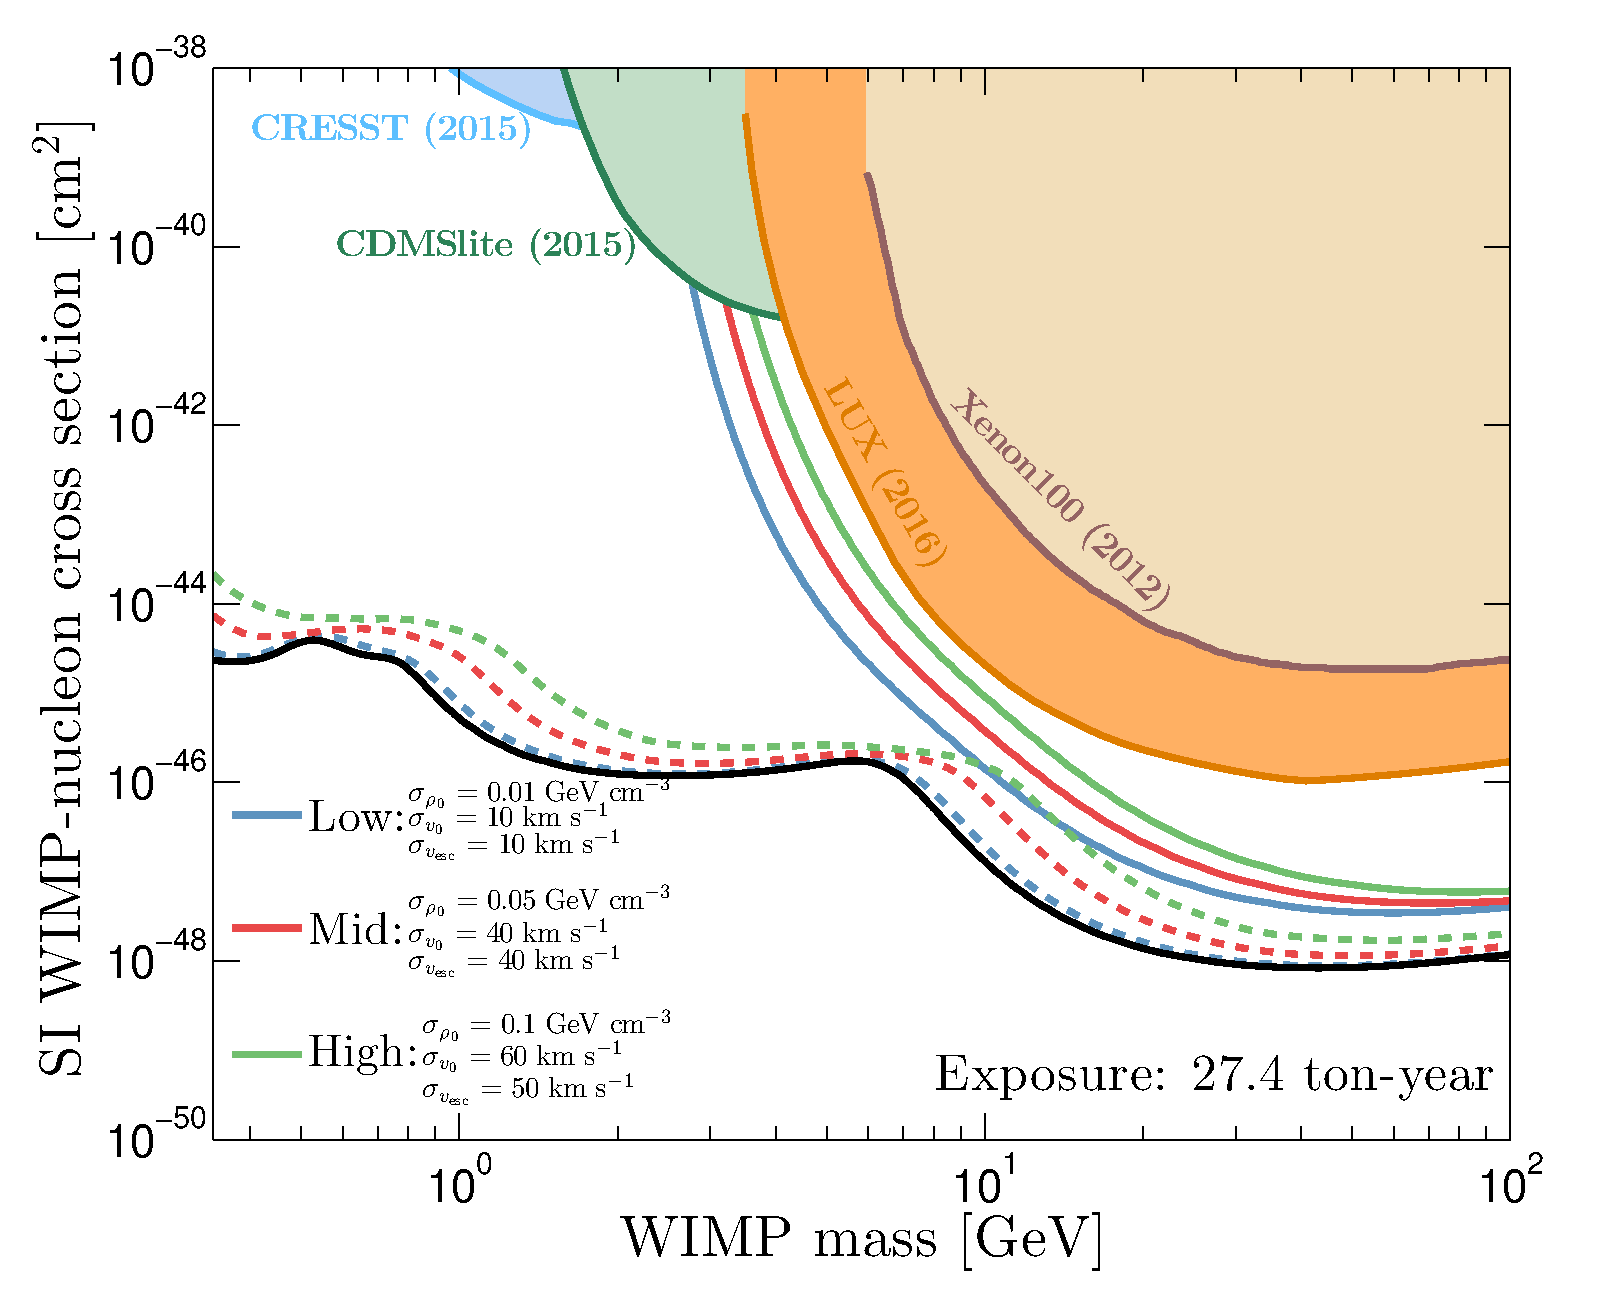
\includegraphics[trim = 0mm 0 0mm 0mm, clip, width=0.8\textwidth,angle=0]{Figures/DL_Resolution.eps}
\caption[Neutrino floor for a realistic detector]{SI discovery limits as a function of WIMP mass for 3 sets of values of the uncertainty placed on the astrophysical parameters: local density, Solar velocity and escape velocity. The blue, red and green curves correspond to low, medium and high values for these uncertainties with 1$\sigma$ values shown. The solid lines are obtained when the detector efficiency is taken into account and the recoil spectrum is convolved with a Gaussian energy resolution with $\sigma(E_r) = 0.8 E_r$ and the corresponding neutrino floors i.e. with no detector effects, are shown as dashed lines. The filled regions are currently excluded by experiments, CRESST~\cite{Angloher:2015ewa}, CDMSlite~\cite{Agnese:2015nto}, Xenon100~\cite{Aprile:2012nq} and LUX~\cite{Akerib:2016vxi}. For comparison we show the neutrino floor calculated without considering astrophysical uncertainties, indicated by the black line.}
\label{fig:DL_Resolution}
\end{center}
\end{figure}
Future direct detection experiments such as Xenon1T~\cite{Aprile:2015uzo} and  LZ~\cite{Akerib:2015cja}, are poised to make the first detection of CNS. So far we have only shown floors that are defined without the consideration of any additional experimental limitations. In practice all detectors suffer from complications such as imperfect energy resolution, efficiency and have thresholds in the $\mathcal{O}(1-10)$ keV range as opposed to the ultra-low thresholds that are used when mapping the low WIMP mass neutrino floor.

We show now discovery limits for a 2 keV threshold xenon detector with a 10 ton target mass over 1000 days running time, a reasonable estimate of the specifications of near future experiments. We include an energy resolution which we take to be 80\% at 1$\sigma$ over the full energy range, i.e. $\sigma(E_r) = 0.8 E_r$. We also take into account the efficiency of the detector which decreases towards the threshold of the experiment. In the following results we assume a simple efficiency curve which increases linearly from 25\% at the threshold energy to 100\% at the maximum energy of 50 keV.

The results of Fig.~\ref{fig:DL_Resolution}, based on this more realistic detector, follow from those of Fig.~\ref{fig:DL_uncertainties}. When the uncertainty on $v_0$ is larger, the floor appears at larger WIMP masses for the same reasons as discussed previously. In this case we see that for the largest uncertainties the discovery limits lie extremely close to existing limits, but have shapes indicating the presence of $\sim$150 $^8$B neutrino events. The inclusion of energy resolution is interesting in this context as it in fact forces some of the neutrino events to be pushed {\it above} the energy threshold of the experiment. However the sensitivity is now also limited by the loss of information due to the smearing of the energy spectrum as well as a reduction in the overall event rate due to the efficiency. So these more realistic limits, despite being subject to a sizable neutrino background, do not yet approach the neutrino floors calculated previously. The general conclusion of Sec.~\ref{sec:nufloor_astro} remains, that larger uncertainty values on the astrophysics content of the WIMP signal weakens the possible constraints that can be made by a future experiment.



\subsection{Parameter constraints}\label{sec:nufloor_parcon}
\begin{figure}
\begin{center}
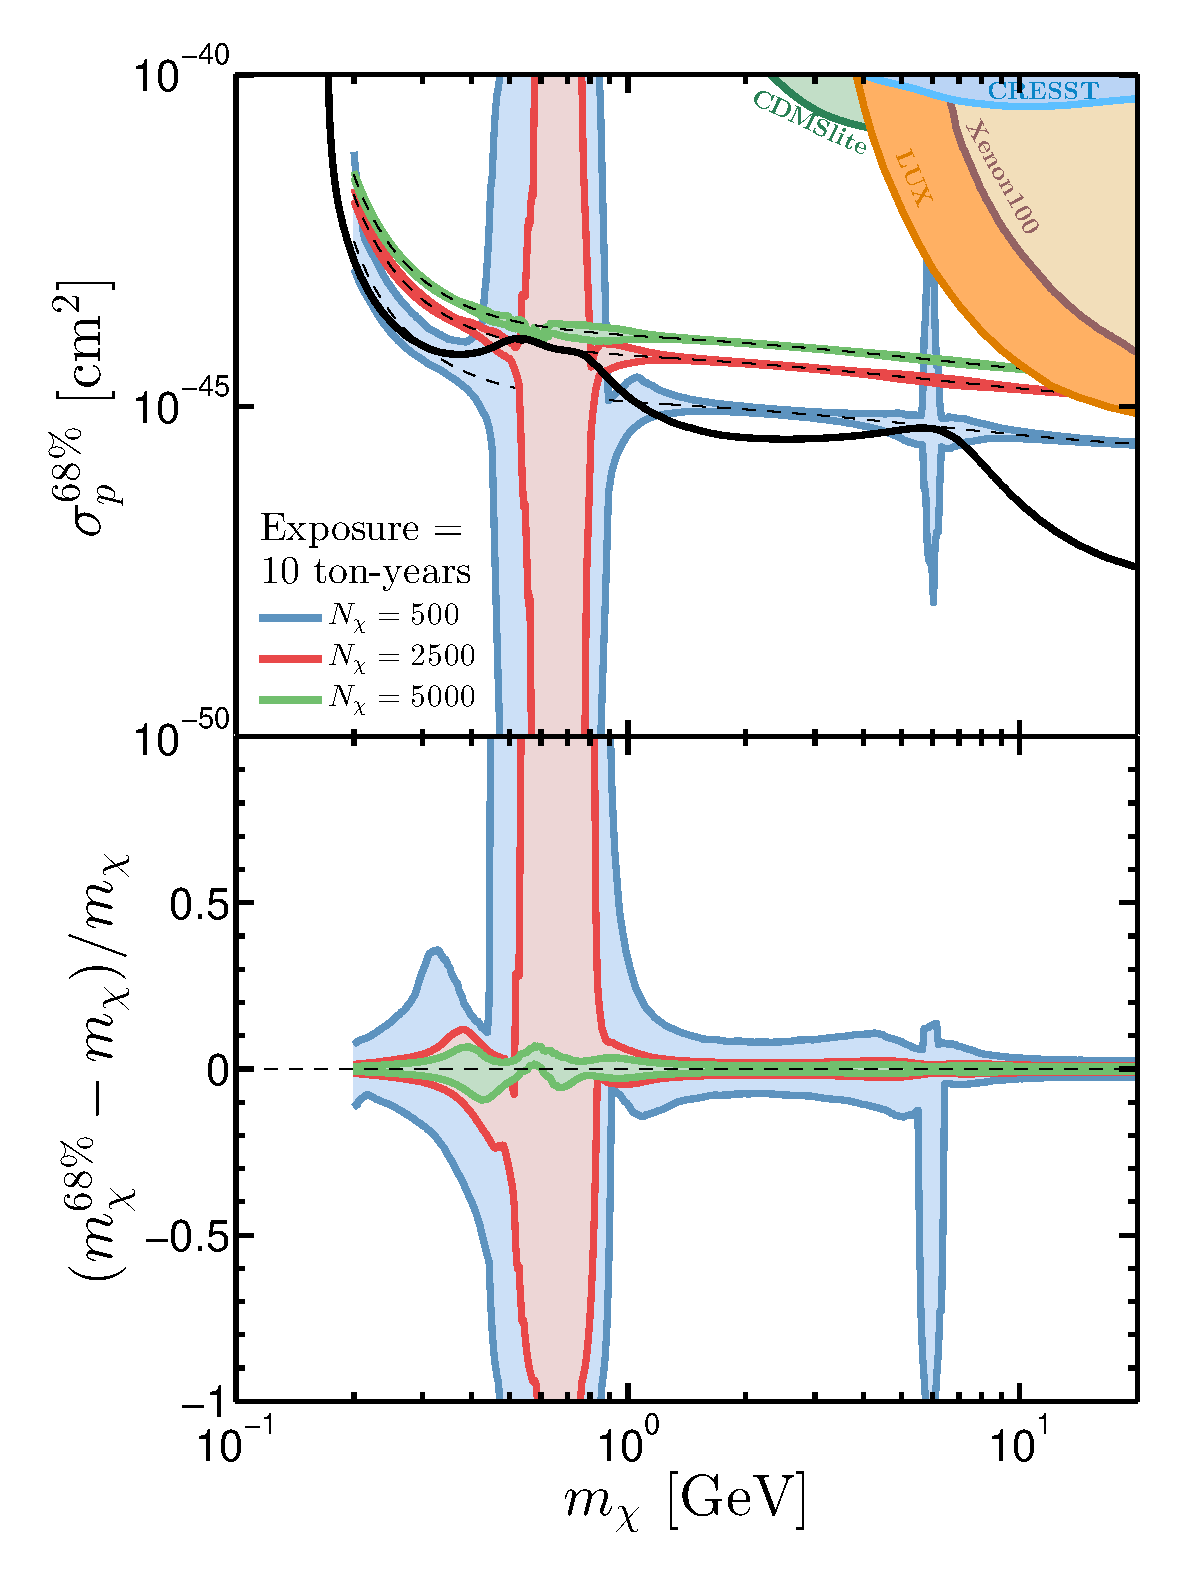
\includegraphics[trim = 5mm 0 0mm 0mm, clip, width=0.49\textwidth,angle=0]{Figures/error_recon.eps}
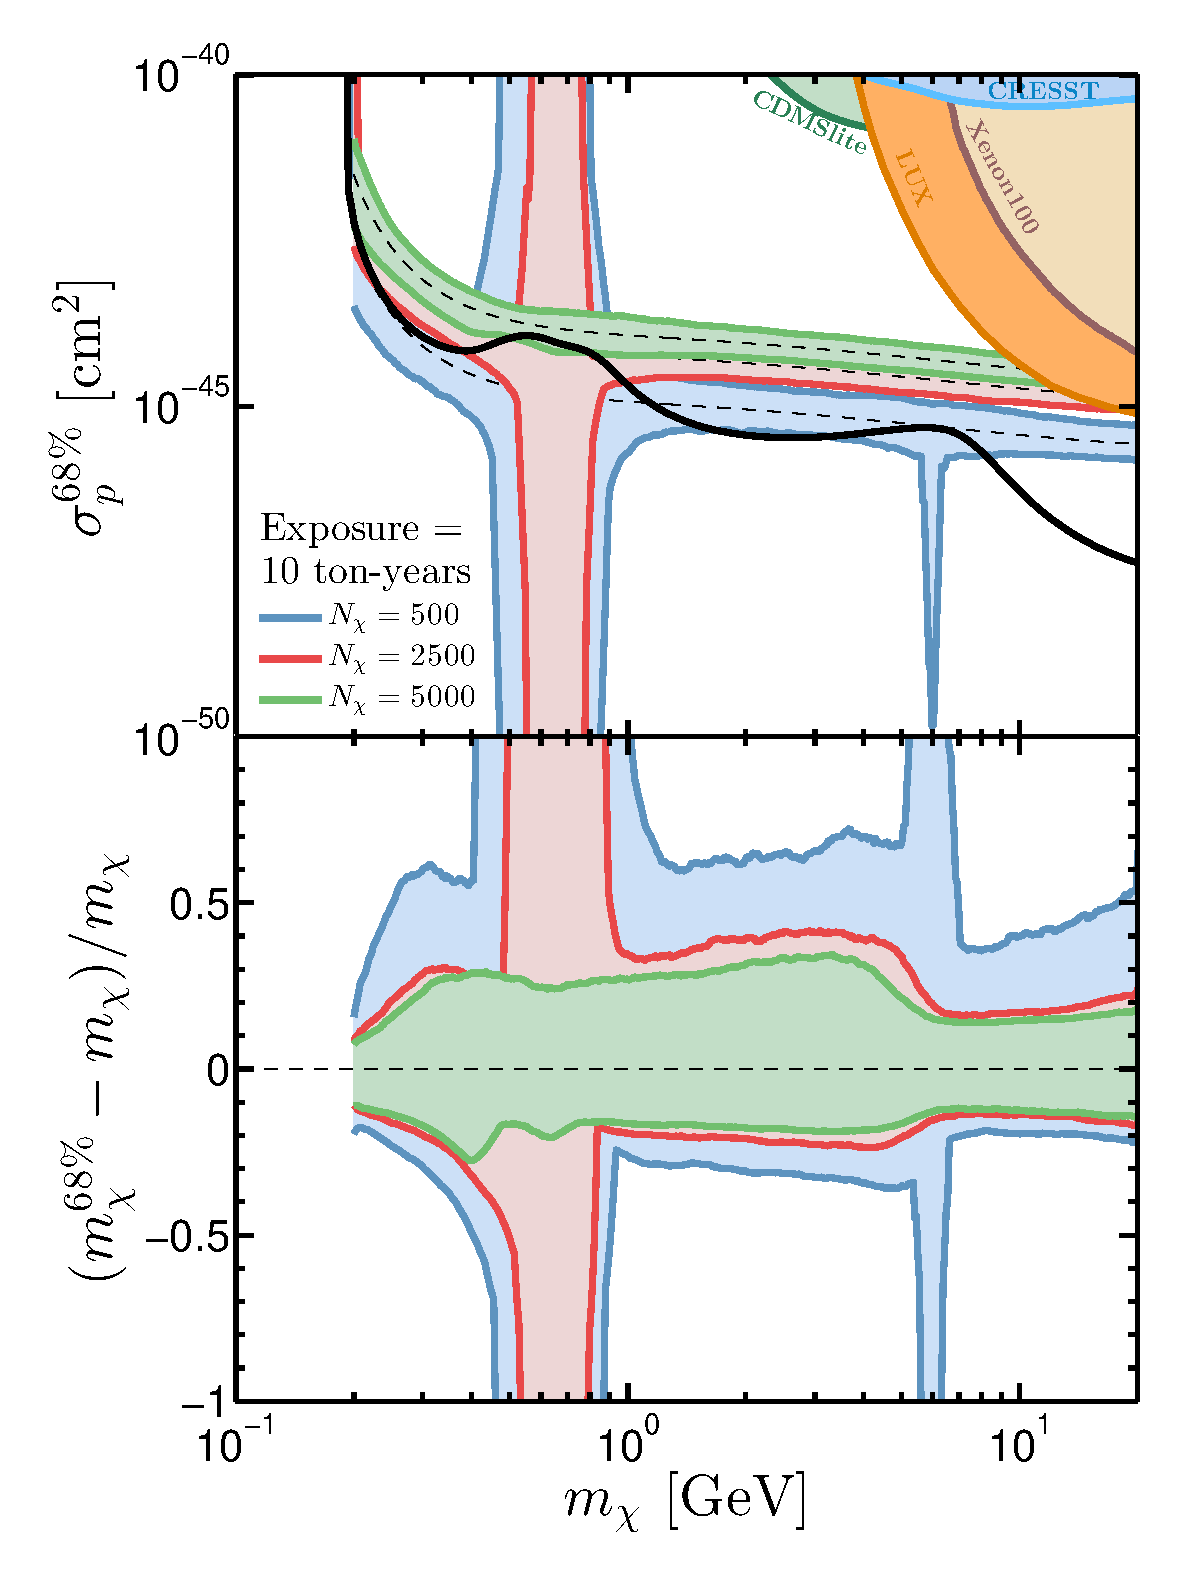
\includegraphics[trim = 5mm 0 0mm 0mm, clip, width=0.49\textwidth,angle=0]{Figures/error_recon_Maxwell.eps}
\caption[Parameters reconstruction under the neutrino background]{{\bf Left:} Reconstructed intervals for $\sigma^{\rm SI}_p$ and $m_\chi$ as a function of input WIMP mass in the presence of the neutrino background. The coloured shaded regions enclose the 68\% confidence intervals on cross section $\sigma^{68\%}_p$ (top panel) and WIMP mass $m^{68\%}_\chi$ (bottom panel, scaled by the input mass $m_\chi$). The input cross section for each WIMP mass is chosen to fix the expected number of WIMP events to 500 (blue), 2500 (red) or 5000 (green). The dashed lines in each region indicate those input values. {\bf Right:} As in the left panel but with $v_0$, $\vesc$ and $\rho_0$ allowed to vary. The filled regions are currently excluded by experiments, CRESST~\cite{Angloher:2015ewa}, CDMSlite~\cite{Agnese:2015nto}, Xenon100~\cite{Aprile:2012nq} and LUX~\cite{Akerib:2016vxi}.}
\label{fig:error_recon}
\end{center}
\end{figure} 
The neutrino floor as derived in the previous section is a convenient way of indicating how much of the WIMP mass-cross section parameter space is accessible to an ideal experiment. However they give us no information with regards to how the ingredient parameters of the WIMP signal may be constrained around this limit, which is undoubtedly a goal of direct detection experiments. To demonstrate this we adopt a similar methodology to the parameter reconstruction introduced in Chapter~\ref{chapter:directional}. We again utilise the nested sampling algorithms provided by {\sc MultiNest}~\cite{Feroz:2007kg,Feroz:2008xx,Feroz:2013hea}, but now exploring the WIMP+neutrino likelihood function, Eq.~(\ref{eq:likelihood}). 

In Fig.~\ref{fig:error_recon} we show the 68\% profile likelihood confidence intervals in the reconstructed values of WIMP mass and cross section, $m^{68\%}_\chi$ and $\sigma^{68\%}_p$. The input values are chosen to produce a fixed number of WIMP events ($N_\chi = 500$, 2500 or 5000 in a 10 ton-year exposure). These lines of constant WIMP event number (shown in Fig.~\ref{fig:error_recon} as dashed lines) are chosen so that they fall either above or below the neutrino floor at various points. For instance the line for $N_\chi= 500$ (green filled region) falls just above the neutrino floor over the full range of WIMP masses, the line corresponding to $N_\chi = 2500$ (red filled region) falls below the floor around 0.6 GeV but above at 6 GeV and the $N_\chi = 5000$ case (blue filled region) falls below the floor around 0.6 GeV and 6 GeV. We can see that input WIMP parameters below the neutrino floor are very poorly reconstructed with 68\% intervals lying outside of the displayed range. However input WIMP parameters above the neutrino floor are reconstructed very well as one would usually expect given the large event numbers. For input values lying on the neutrino floor, for instance at 6 GeV, we see a sharp increase in the error on the reconstructed mass and cross section. 

In the right hand panel of Fig.~\ref{fig:error_recon} we show the results for the same analysis as in the left hand panel but now with the astrophysical parameters unfixed in the likelihood function. For each set of inputs we see a large increase in the recovered intervals across the mass range. We can attribute the increase in error on $\sigma^{\rm SI}_p$ to the additional uncertainty in the expected number of events due to $\rho_0$ and $v_0$. The increase in the $m_\chi$ interval is largely due to the uncertainty on $v_0$ which in particular leads to a huge increase in reconstructed intervals around 6 GeV for the case when $N_\chi = 500$. Following the conclusion of Sec.~\ref{sec:nufloor_astro} which found that accounting for astrophysical uncertainties prohibited a larger range of WIMP parameter values from being accessed, similarly here the inclusion of astrophysical uncertainties has a detrimental effect on the measurement of those parameter values. It is well known that a good understanding of the astrophysics dependence of the WIMP signal is crucial for making measurements of WIMP properties, however this is especially true when neutrinos are the dominant background.

\section{Circumventing the neutrino floor}\label{sec:nufloor_time}
So far we have discussed the phenomenology and shape of the neutrino floor limit itself. Clearly the salient issue is how experiments may search for dark matter in the presence of an ``irreducible'' neutrino background. In other words we want to access cross sections {\it below} the neutrino floor. Perhaps due to the name, the neutrino floor is often misinterpreted as a hard limit to the discoverability of dark matter via direct detection. However the neutrino background is not strictly irreducible. As we described in Sec.~\ref{sec:nufloor_nufluxunc} the `floor' can be conquered with high statistics thanks to the small differences between the WIMP and neutrino recoil spectra. However these high statistics are likely unobtainable by any future experiment so to progress at a more reasonable rate past the neutrino floor we would ideally like to search for some other distinguishing features.

\subsection{Time dependence}
\begin{figure}
\begin{center}
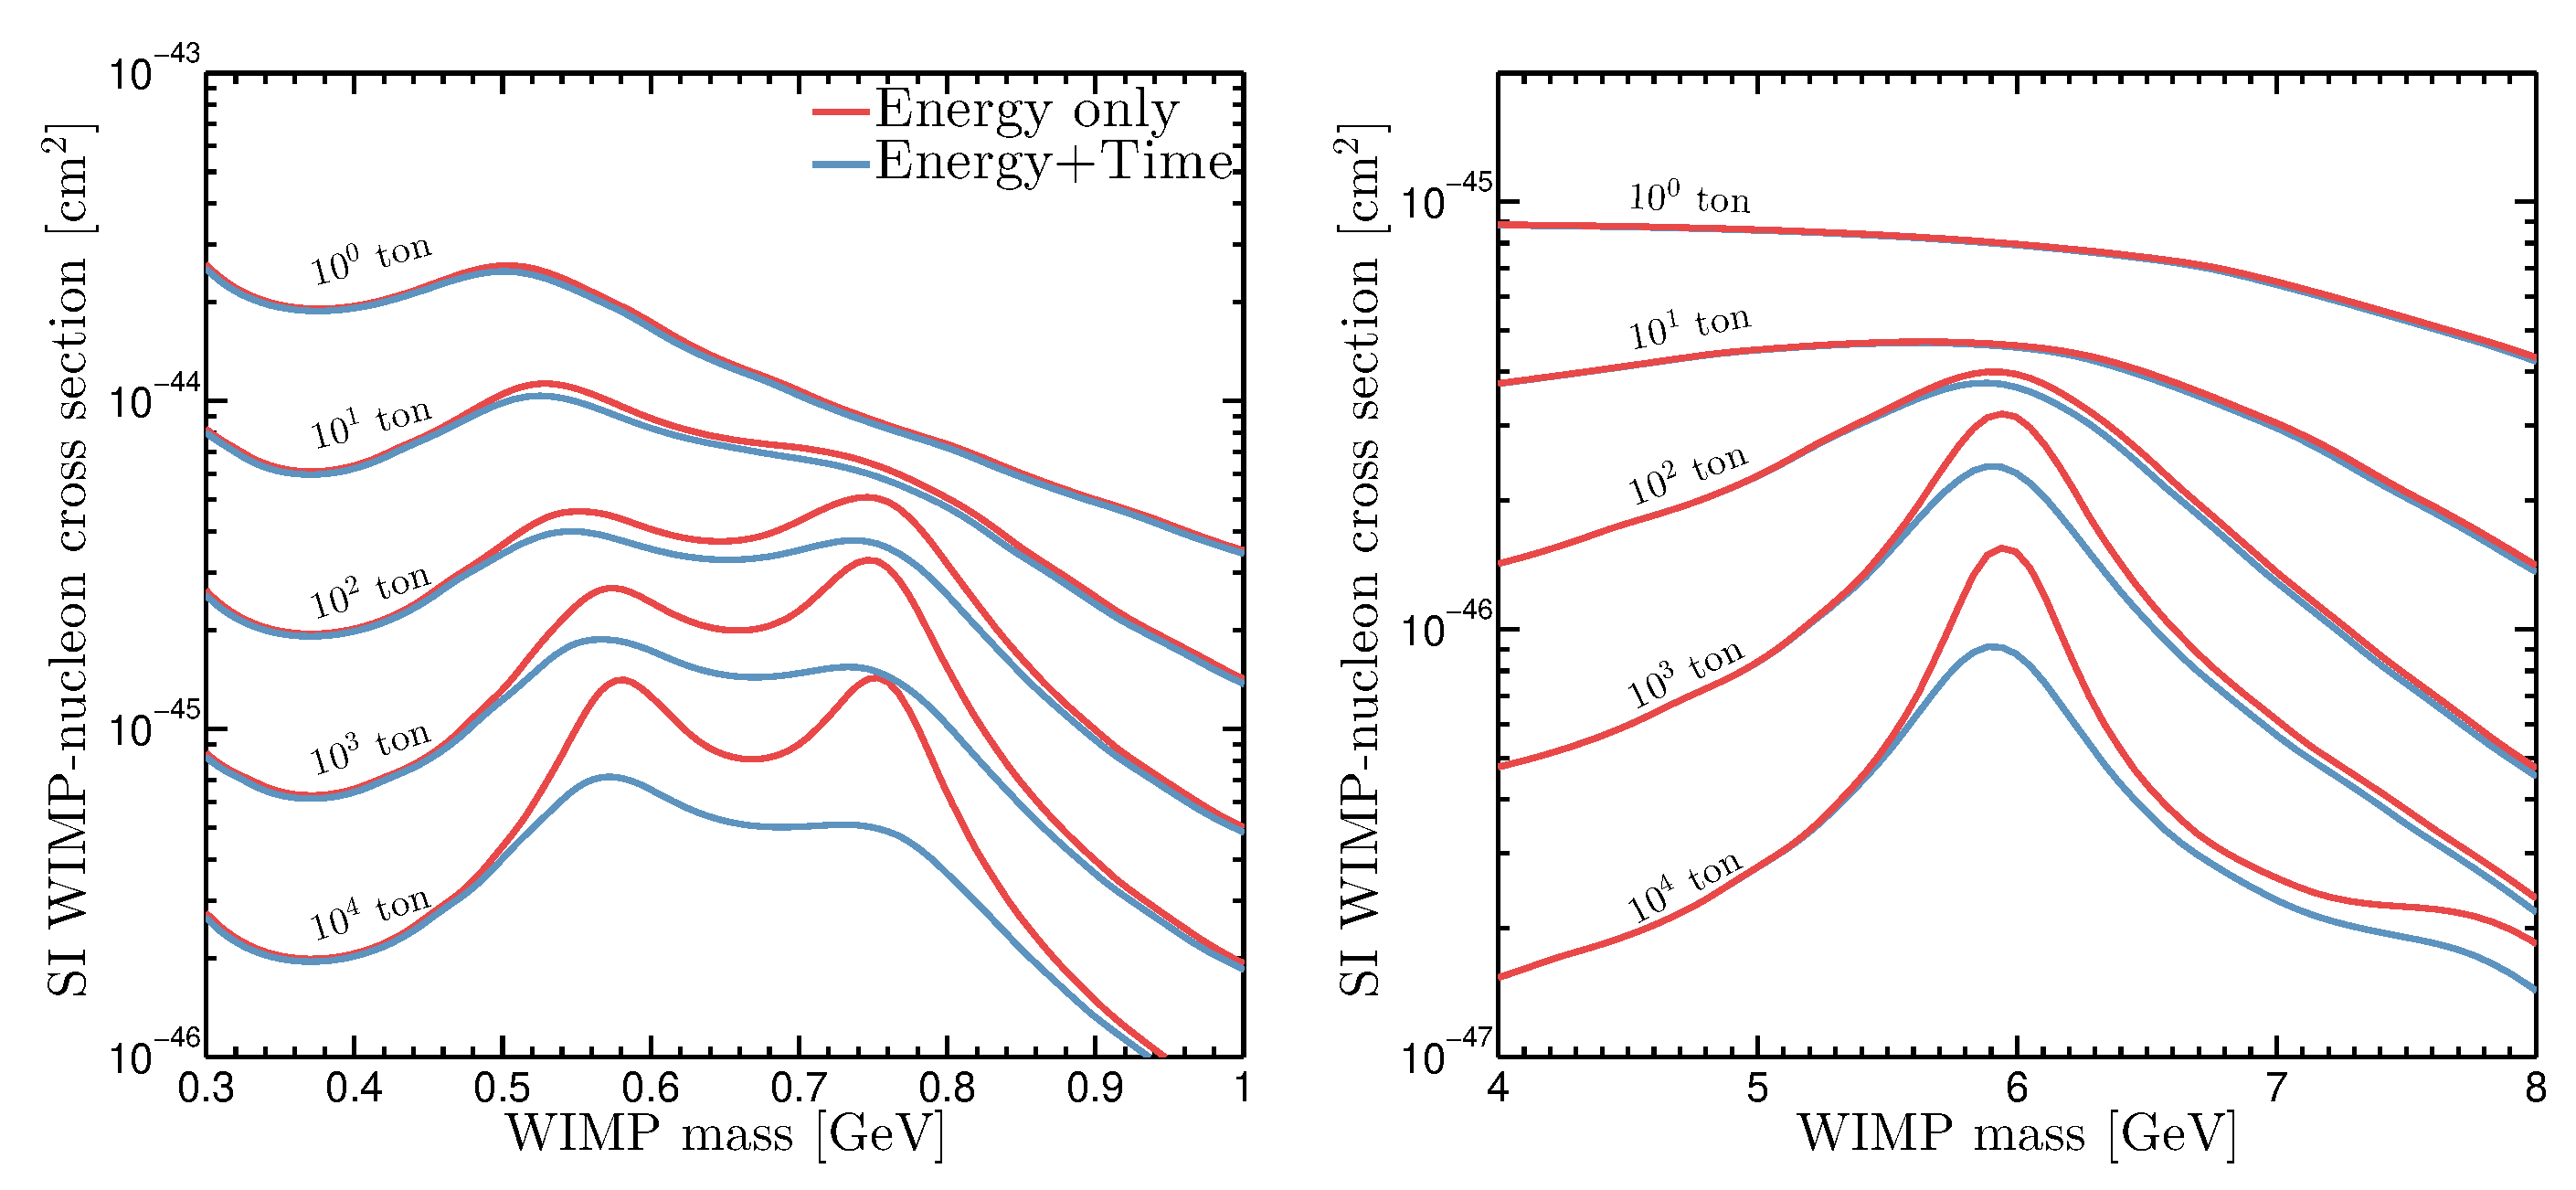
\includegraphics[trim = 0mm 0mm 0mm 0mm, clip,width=\textwidth,angle=0]{Figures/DL_Time.eps}
\caption[Neutrino floor evolution with timing information]{SI neutrino floor evolution in the $0.3 - 1$~GeV ({\bf left}) and $4 - 5$~GeV mass range ({\bf right}). The red curves show the bounds obtained when only energy information is considered and the blue shows the improvement when time information is added. There are four sets of curves shown for detector masses from 1 ton to 10$^4$ tons (top to bottom). In each case the exposure time was kept at a constant 1 year from the 1st of January 2016.} 
\label{fig:DL_Time}
\end{center}
\end{figure}
It was shown in Ref.~\cite{Davis:2014ama} that the time dependence of the WIMP and Solar neutrino event rates provides a distinguishing feature between the two signals which can help circumvent the neutrino floor with fewer events than a recoil energy only analysis. In Fig.~\ref{fig:DL_Time} we show the improvement on the neutrino floor limit after the inclusion of timing information. We show only narrow mass ranges: between 0.3 - 1 GeV when the floor is induced by $^7$Be, $pep$, $^{13}$N, $^{15}$O and $^{17}$F neutrinos and between 4 - 8 GeV due to $^8$B and $hep$ neutrinos. Outside of these specific mass ranges (for the exposures considered here) the improvement offered by time information is negligible. The advantage of including timing information is that in practice, the time tagging of events is often trivial and is common in many experimental configurations. However, because the annual modulation amplitudes are small, obtaining a benefit from time information (over simply not including it) needs in excess of $\mathcal{O}(1000)$ neutrino events. It is clear that to probe further below the neutrino floor we require signals to discriminate between neutrinos and dark matter in a much more pronounced way.




\subsection{Direction dependence}\label{sec:nufloor_res} 
The power of a directional experiment in the context of the neutrino background is fundamentally going to be controlled by the differences in the angular pattern of recoils across the sky\footnote{We do not explore the possibility here, but it may be the case that directional effects can give rise to discrimination between neutrinos and WIMPs in experiments that do not observe recoil tracks, e.g. with spin-polarised $^3$He~\cite{Franarin:2016ppr}.}. The essential aspect that one desires for background rejection is some region of dataspace in which one expects only signal events and no background events. As we have already displayed in Fig.~\ref{fig:Moll} in the full 3-dimensional recoil spectrum such a signal region does exist and is visible by eye. This consideration naturally leads us to contemplate lower dimensional readout scenarios as these will have drastically different angular distributions. Moreover, readout technologies are a principle experimental concern for current directional detection strategies~\cite{Battat:2016pap}. In the following results we will extend beyond the ideal cases of Chapter~\ref{chapter:directional} and consider a range of experimental factors: lower dimensional recoil track projections, head-tail recognition, and finite angular resolution.

We will consider a detector with the $\hat{{\bf x}}$,  $\hat{{\bf y}}$, and $\hat{{\bf z}}$ axes pointing toward the North, the West and the Zenith directions respectively. In the detector frame, the direction of a recoil is given by the angles $\theta$ and $\phi$ defined such that,
\begin{equation}
\hat{{\bf q}} = \sin\theta\cos\phi \, \hat{{\bf x}} + \sin\theta\sin\phi \, \hat{{\bf y}} + \cos\theta \, \hat{{\bf z}} \,.
\label{eq:angles}
\end{equation}

To relate to previous results and the larger literature on the neutrino floor we again focus on a xenon-based experiment. We locate the detector at Modane with latitude and longitude (45.2$^\circ$,~6.67$^\circ$), taking data over a duration $\Delta t = 1$~year. 

For computational efficiency we use now an {\it unbinned} likelihood function,
\begin{equation}
\mathscr{L}(m_\chi,\sigma^{\rm SI}_p,\boldsymbol{\Phi}) = \frac{e^{-(N_\chi+\sum_{j=1}^{n_{\nu}}N^j_\nu)}}  {N_{\rm obs}!} \prod_{i=1}^{ N_{\rm obs}}\left[N_\chi f_\chi(\textbf{d}^i) + \sum_{j=1}^{n_{\nu}}N^j_\nu f^j_\nu(\textbf{d}^i)\right] \prod_{k=1}^{n_{\nu}}\mathscr{L}_k(\Phi_k) \,,
\end{equation}
where the index $i$ runs over the $N_{\rm obs}$ events and the indices $j$ and $k$ relate to the $n_\nu$ neutrino backgrounds. We use $N_\chi$ and $N^j_\nu$ for the expected number of WIMP and neutrino events respectively. We now introduce $f_\chi(\textbf{d}^i)$ and $f_\nu^j(\textbf{d}^i)$ for the WIMP and neutrino event distributions at data point $\textbf{d}^i$ which will have a dimensionality corresponding to the number of observables in the experiment. We compare six strategies:
\begin{itemize} \itemsep0em 
 \item 3-d directional readout, $\textbf{d} = \{E_r,\theta,\phi,t\}$
 \item 2-d directional readout, $\textbf{d} = \{E_r,\phi,t\}$
 \item 1-d directional readout, $\textbf{d} = \{E_r,\theta,t\}$
 \item No directional information $\textbf{d} = \{E_r,t\}$
 \item Event time only $\textbf{d} = \{t\}$
 \item Number of events only (i.e. a counting experiment) $f_\chi = f^j_\nu = 1$
\end{itemize}
The 3-d directional readout, $\{E_r,\theta,\phi,t\}$, corresponds to the optimum detector that measures and exploits all the information available, e.g.~a low pressure gaseous TPC. For a 2-d readout, $\{E_r,\phi,t\}$ only a 2-dimensional ($x$,$y$) projection of the drifted electron cloud can be measured (e.g.~in a CCD readout TPC); and in 1-d, $\{E_r,\theta,t\}$, only a measurement of the projection of the recoil track along the drift ($z$) direction (e.g. with columnar recombination).

The last two strategies we list correspond to detectors that can only measure the total number of events above some threshold. This is the case for bubble chamber experiments~\cite{Cushman:2013zza} that adjust their operating pressure to nucleate a single bubble from a nuclear recoil. Such experiments would have very poor inherent background rejection capabilities, but they are an informative benchmark to consider in this comparative study. The energy and time, $\{E_r,t\}$, strategy corresponds to the majority of current and ongoing direct detection experiments.

\begin{figure}
\begin{center}
%\includegraphics[width=\textwidth,angle=0]{Figures/Daily_1D2D_evolution-eps-converted-to.pdf}
\includegraphics[trim = 0mm 0 0mm 0mm, clip, width=0.99\textwidth]{Figures/Daily_1D2D_evolution.eps}
\caption[Daily evolution of recoils from ${}^{8}\rm{B}$ neutrinos and WIMPs]{The daily evolution, at three hourly intervals, of the angular distributions of 0.5 keV xenon recoils from
${}^{8}\rm{B}$ neutrinos (left column) and a WIMP with mass $m_{\chi} = 6 \, {\rm GeV}$ (right). The distributions are normalised to unity in each case and displayed with arbitrary units. The top row shows the distribution of $\cos{\theta}$  measured by a detector with 1-d readout and the bottom row the angle $\phi$  for  2-d readout. The date chosen was September 6th, when the angular separation between Cygnus and the Sun is maximised.} 
\label{fig:daily1d2d}
\end{center}
\end{figure} 
Figure~\ref{fig:daily1d2d} shows the daily evolution of the 1-d ($\cos{\theta}$), and 2-d ($\phi$), recoil angle distributions at a single energy ($E_r~=~0.5$~keV) from ${}^{8}\rm{B}$ neutrinos and a WIMP with mass $m_{\chi} = 6 \, {\rm GeV}$. The $\phi$ distributions from $^8$B neutrinos have two peaks, because at a fixed recoil energy the neutrino energy spectrum produces recoils in a ring around the incident direction. In the WIMP case, however, the distribution of recoils is peaked in a single direction, towards $-\textbf{v}_\textrm{lab}$. The 2-d and 1-d distributions for both atmospheric and DSNB neutrinos are flat, and therefore we do not show them for clarity. The WIMP and neutrino distributions are significantly different, not only in their shape at a single time but also how they evolve over the course of a day. This suggests that a detector with only 1-d or 2-d readout should still be able to discriminate WIMP and neutrino induced recoils.


\begin{figure}
\begin{center}
\includegraphics[trim = 0mm 0mm 0mm 0mm, clip,width=0.49\textwidth,angle=0]{Figures/SI_discovery_Xe_6GeV.eps}
\includegraphics[trim = 0mm 0mm 0mm 0mm, clip,width=0.49\textwidth,angle=0]{Figures/SI_discovery_Xe_100GeV.eps}
\caption[Neutrino floor vs detector mass for different readout strategies]{The dependence of the discovery limit for the SI WIMP-nucleon cross section on the mass of a xenon detector operated for $1 \, {\rm year}$ using  (from top to bottom) 
the number of events only (pink line), time information (brown dashed),  energy \& time (orange dashed), energy \& time  plus 1-d (red), 2-d (blue) and 3-d (green) directionality. 
The left (right) plot is for $m_{\chi} = 6 \, (100) \, {\rm GeV} $ and an energy threshold $E_{\rm th} = 0.1 \, (5) \, {\rm keV}$ and the bottom axis shows the number of ${}^{8}\rm{B}$  (atmospheric) neutrinos expected. 
Note the different scales of the left and right hand plots.} 
\label{fig:detectormass}
\end{center}
\end{figure}

Figure~\ref{fig:detectormass} shows the evolution of the SI discovery limit with increasing detector mass, $M$, using each of the six different readout strategies. We consider two example WIMP masses and detector: a light WIMP \&  low threshold detector ($m_{\chi} = 6$ GeV and $E_{\rm th} = 0.1$ keV) and a 100 GeV WIMP \&  moderate threshold detector ($E_{\rm th} = 5 $ keV). For these two WIMP masses the recoil energy spectra closely matches those of $^8$B and atmospheric neutrinos respectively. It should be emphasised that these thresholds by the standards of directional detectors are very low. However the purpose of this study is to establish whether the neutrino background can be subtracted using directional information, rather than by some specific detector. Indeed, a detector with a threshold above $\sim$5~keV observes no Solar neutrino background at all, so the point is somewhat inconsequential unless we use low thresholds. We note also that there have been methods proposed to look for directional effects in very low energy signals using semiconductors~\cite{Kadribasic:2017obi}.

The evolution of the discovery limit develops as a function of $M$ (or equivalently neutrino event number) in a number of phases as we have already described in Sec.~\ref{sec:nufloor_nufluxunc}. Notably, when the expected number of neutrino events reaches $10-10^{2}$ the counting only, time only, as well as the energy \& time limits all plateau\footnote{Interestingly we see that timing information here seems to be more useful for discriminating Solar neutrinos from light WIMPs than for discriminating atmospheric neutrinos from heavier WIMPs. We can attribute this to the fact that the WIMP and Solar neutrino rates are both annually modulated, and also the amplitude of the annual modulation is larger for lighter WIMPs (cf. Fig.~\ref{fig:AnnualDailyModulation}).}. The limits with directional readout however continue to decrease as the incorporation of directional information allows the distributions of WIMP and neutrino induced recoils to be distinguished. For the 100 GeV WIMP case, the limits from 2-d and 3-d readout are a factor of $\sim 1.2$ and $1.6$ better than those from 1-d readout whereas for the 6 GeV WIMP case they are factors of $\sim 1.2$ and $3$ times better. The discovery limit with directionality continues to decrease as $\propto 1/M$ for the 6 GeV WIMP as the directional and time-dependent distributions of the WIMP and Solar neutrino induced recoils have such a small overlap that the background has very little effect on the discovery capabilities of the experiment. However for the 100 GeV WIMP the dominant background from atmospheric neutrinos significantly overlaps with the WIMP distribution so, although the experiment is able to distinguish the WIMP signal, the sensitivity is still compromised by the background. In this case the discovery limit, beyond the saturation regime, evolves according to a standard Poisson background subtraction mode $\propto 1/\sqrt{M}$.

\begin{figure}
\begin{center}
\includegraphics[width=0.8\textwidth,angle=0]{Figures/ReadOut_Comparison_floors.eps}
\caption[Comparison of discovery limits with different readout strategies]{%The discovery limit for the spin independent WIMP-nucleon cross section, $\sigma_{\rm p}^{\rm SI}$, as a function of WIMP mass for a ${\rm Xe}$ detector operated for $1 \, {\rm year}$ 
The discovery limit
%, as in Fig.~\ref{fig:detectormass},
as a function of WIMP mass using (from top to bottom): time information (brown dashed),  energy \& time (orange dashed), 1-d (red), 2-d (blue) and 3-d (green) directionality. 
The upper (lower) set of lines are for the detector set-up with target mass $M=0.1 \, (10^4)$ tons and threshold $E_{\rm th} = 0.1 \, (5) \, {\rm keV}$. 
The orange region shows the neutrino floor from Ref.~\cite{Ruppin:2014bra}. The grey region covers parameters already excluded by experiments.} 
\label{fig:readoutfloors}
\end{center}
\end{figure} 

Having studied the evolution of the discovery limit as a function of detector mass for two specific WIMP masses, we now consider two fixed example detector set-ups: a low mass \& low threshold detector ($M=0.1$ ton and $E_{\rm th} = 0.1 \, {\rm keV}$ respectively) and a high mass \& moderate threshold detector ($10^4$ ton and 5 keV). These detector masses and thresholds are chosen so that a non-directional detector with the same mass and threshold would be in the saturation regime that results in the neutrino floor, as seen in Fig.~\ref{fig:detectormass}. Figure~\ref{fig:readoutfloors} shows the discovery limit as a function of WIMP mass for these two detector set-ups and each readout strategy. Also shown as the orange shaded region is the well known neutrino floor from Ref.~\cite{Ruppin:2014bra} which is the concatenation of two separate limits roughly matching our two detector setups\footnote{For light WIMPs ($m_{\chi} <10$ GeV) the limit comes from a 3 eV threshold detector with an exposure of 0.19 ton years, while for heavier WIMPs ($m_{\chi} >10$ GeV) a detector with a 4 keV threshold and an exposure of $9.3 \times 10^3$ ton years was used.}.

For the low threshold detector, the directional discovery limits clearly cut through the light WIMP neutrino floor and for the 3-d readout there is almost no reduction in sensitivity due to the neutrino background. The 1-d and 2-d readouts do suffer a small reduction in sensitivity, but evidently the distributions are different enough that it is still possible to probe cross sections below the limit set by non-directional experiments. For the high threshold detector the improvement in the discovery limits, with respect to the high-mass neutrino floor, from directionality is smaller. However it does still help discriminate the isotropic atmospheric neutrino background from WIMP induced recoils, in particular for WIMP masses around $100 \, {\rm GeV}$ where the energy spectra from WIMPs and atmospheric neutrinos are most similar.

In summary, we find that directionality is a powerful tool for disentangling neutrino backgrounds from a WIMP signal. The gain from directionality is particularly impressive for low mass WIMPs thanks to the large separation between the Solar neutrino and WIMP incoming directions (cf. Sec.~\ref{sec:nufloor_signals}). We also find that this result still holds even if only the 2-d or 1-d projection of the recoil tracks can be measured.


\subsection{Non-ideal detectors}\label{sec:nufloor_nonideal}
\label{sec:nufloor_sense}
\begin{figure}
\begin{center}
\includegraphics[width=0.8\textwidth,angle=0]{Figures/HeadTail_combined.eps}
\caption[Neutrino floor as a function of head-tail discrimination threshold]{
The discovery limit as a function of the energy threshold for head-tail discrimination for 1-d (red), 2-d (blue) and 3-d (green) directional readout (with energy and time information in all three cases). The dashed orange line shows the discovery limit with energy information only.
The left (right) set of lines correspond to the discovery limits at 6 (100) GeV made by the detector set-up with target mass $M=0.1 \, (10^4)$ tons and threshold $E_{\rm th} = 0.1 \, (5) \, {\rm keV}$. }
%a detector with a target mass $M=0.1 \, (10^4)$ ton and an energy threshold $E_{\rm th} = 0.1 \, (5) \, {\rm keV}$.} 
\label{fig:headtail}
\end{center}
\end{figure} 

\begin{figure}
\begin{center}
\includegraphics[width=0.8\textwidth,angle=0]{Figures/HeadTail_floors.eps}
\caption[Neutrino floor for directional detectors with no sense recognition]{The discovery limit as a function of WIMP mass for detectors with full sense recognition (solid lines) and no sense recognition (dashed) and 1-d (red), 2-d (blue) and 3-d (green) directional readout. The upper (lower) set of lines are for the detector set-up with target mass $M=0.1 \, (10^4)$ tons and threshold $E_{\rm th} = 0.1 \, (5) \, {\rm keV}$. The dashed orange lines show our discovery limit with energy information only and
the orange region shows the neutrino floor from Ref.~\cite{Ruppin:2014bra}. The grey region covers parameters already excluded by experiments.}
\label{fig:headtailfloors}
\end{center}
\end{figure} 

\begin{figure}
\begin{center}
\includegraphics[trim = 0mm 0mm 0mm 0mm,clip,width=0.49\textwidth,angle=0]{Figures/HeadTail_sig_vs_Exposure_6GeV.eps}
\includegraphics[trim = 0mm 0mm 0mm 0mm,clip,width=0.49\textwidth,angle=0]{Figures/HeadTail_sig_vs_Exposure_100GeV.eps}
\caption[Neutrino floor vs detector mass with no sense recognition]{The dependence of the discovery limit for the SI WIMP-nucleon cross section on detector mass for detectors with (solid lines) and without (dashed lines) sense recognition for each of the three directional readout strategies 3-d (green), 2-d (blue) and 1-d (red). The discovery limit for energy + time only readout is shown with the orange lines. The left (right) panel is for 
$m_{\chi} = 6 \, (100) \, {\rm GeV} $ and detector set-up with threshold $E_{\rm th} = 0.1 \, (5) \, {\rm keV}$. \label{fig:headtailmass}}
%The dependence is shown for the same two WIMP mass cases as in Fig.~\ref{fig:detectormass}, left: 6 GeV (with a 0.1 keV threshold), and right: 100 GeV (with a 5 keV threshold).} 
\end{center}
\end{figure}

We now move beyond the ideal situation and consider two limitations particular to directional experiments: head-tail (sense) recognition and angular resolution. 

{\bf Head-tail recognition}, as we have already discussed, is one of the most important considerations for the discovery reach of directional experiments. Head-tail effects based on charge deposition or track geometry are naturally more apparent at larger recoil energies. Figure~\ref{fig:headtail} shows how the discovery limit depends on the {\it threshold} for head-tail discrimination.
For simplicity, we assume that below the head-tail energy threshold there can be no sense discrimination.
For the light WIMP and the low mass and threshold detector, the discovery limits are weakened as the head-tail energy threshold is increased from $0.1 \, {\rm keV}$ to $\sim 1-2 \, {\rm keV}$ before flattening off to a factor between $\sim 1.5$ (for 1-d)  and $\sim 10$ (for 3-d) below the energy only limit. For lower dimensional readout the decrease in sensitivity is larger and the plateau in the limit is reached for a larger head-tail energy threshold. Qualitatively similar behaviour occurs for the $100 \, {\rm GeV} $ WIMP and the higher mass and threshold detector. In this case the discovery limits flatten off to values $1.1 - 1.2$ below the
energy only limit at a head-tail energy threshold of $60 \, {\rm keV}$. 

In Figure~\ref{fig:headtailfloors} we show the discovery limits with and without sense recognition, as a function of WIMP mass. The factor by which the discovery limit changes without sense recognition is largest for light, $m_{\chi} < {\cal O}(20 \, {\rm GeV})$, WIMPs and a low threshold. The discovery limit achieved by a 3-d readout is still considerably lower than the non-directional limit however 1-d and 2-d readouts do suffer without sense recognition and are only marginally better than the non-directional limits, especially at high WIMP masses.

In Figure~\ref{fig:headtailmass} we show (in similar fashion to Fig.~\ref{fig:detectormass}) the evolution of the discovery limit now as a function of detector mass for $m_{\chi} = 6$ and $100 \, {\rm GeV} $ with and without sense.
As in Fig.~\ref{fig:headtailfloors}, we see that the lack of sense recognition is most damaging in the 100 GeV WIMP case. This is particularly true for the 1-d and 2-d readouts, with no sense recognition there is only a factor of 1.1 and 1.2 improvement over a detector with no directional information at all and the evolution of the discovery limit suffers from a similar (but less severe) saturation effect due to the overlapping recoil distributions. In the 6 GeV WIMP case the discovery limits with no sense recognition continue to decrease past the saturation regime suffered by the non-directional limit. However there is still a reduction in sensitivity by factors of 1.9, 2.8 and 8.9 for 3-d, 2-d and 1-d readouts respectively compared to the limits with sense recognition. Interestingly, the discovery limit for 3-d readout with no sense recognition is slightly better than 1-d and 2-d readouts with sense recognition. 

Our main conclusion regarding sense recognition is that for discriminating between Solar neutrinos and low mass WIMPs, having 3-d readout with no method of determining sense is marginally preferable to 1-d or 2-d readout with sense determination. 
This is because the recoil distributions from low mass WIMPs and Solar neutrinos are both anisotropic and have sufficient 3-d angular separation that they are still distinguishable even without recoil sense information. For the higher mass WIMPs this is not the case, and 
without sense recognition the advantage of directionality is almost entirely lost, even in 3-d.


{\bf Angular resolution} is limited by the inaccuracy in the estimation of the ``true'' recoil direction. This is an inherent difficulty faced by all directional detectors. Finite angular resolution will smear out the WIMP and Solar neutrino distributions in Fig.~\ref{fig:Moll}, making it more difficult to discriminate between the two. Since the minimum separation between the peak WIMP and neutrino directions is $\sim60^\circ$, an angular resolution better than this will likely be required to differentiate between the WIMP and Solar neutrino distributions.

Finite angular resolution results in a recoil in the direction $\hat{\textbf{q}}'(\Omega'_r)$ reconstructed in the direction $\hat{\textbf{q}}(\Omega_r)$ with a probability distribution that takes the form of a Gaussian smoothing kernel on a sphere~\cite{Copi:2005ya,Billard:2011zj}
\be
K(\Omega_r,\Omega_r') = \frac{1}{ (2\pi)^{3/2} \sigma_\gamma \rm{erf}(\sqrt{2}\sigma_\gamma)   } \exp{\left( - \frac{\gamma^2}{2\sigma_\gamma^2} \right)} \,,
\ee
where $\gamma$ is the angle between the original and reconstructed directions,
\be
\cos{\gamma} = \hat{\textbf{q}}'\cdot\hat{\textbf{q}} = \sin{\theta}\sin{\theta'}\cos{(\phi-\phi')} + \cos{\theta}\cos{\theta'}\,,
\ee
in the coordinates defined in Eq.~(\ref{eq:angles}). The measured directional recoil rate is then the convolution of the smoothing kernel with the original directional recoil rate
\be
\frac{{\rm d}^2 R}{\rm{d} \Omega_r \rm{d}E_r} = \int_{\Omega'_r} \frac{{\rm d}^2 R}{\rm{d} \Omega'_r \rm{d}E_r} K(\Omega_r,\Omega'_r) \, {\rm d} \Omega'_r \,.
\ee
\begin{figure}
\begin{center}
\includegraphics[width=0.8\textwidth,angle=0]{Figures/AngRes_100GeV_6GeV-eps-converted-to.pdf}
\caption[The discovery limit as a function of angular resolution]{ The discovery limit as a function of angular resolution, $\sigma_\gamma$ for a detector with 3-d readout.  
The upper (lower) set of lines are for $m_{\chi} = 6 \, (100) \, {\rm GeV}$. The upper (lower) line is for the detector set-up with threshold $E_{\rm th} = 0.1 \, (5) \, {\rm keV}$.   
The dashed lines show the discovery limit using energy information only. }
\label{fig:angressingle}
\end{center}
\end{figure} 

\begin{figure}
\begin{center}
\includegraphics[width=0.8\textwidth,angle=0]{Figures/AngRes_floors.eps}
\caption[Neutrino floor as a function of angular resolution]{The discovery limit, as in Fig.~\ref{fig:readoutfloors}, as a function of WIMP mass with angular resolution, $\sigma_\gamma$, varying between $0^{\circ}$ and $60^{\circ}$ for a detector with 3-d readout. 
The upper (lower) set of lines are for the detector set-up with target mass $M=0.1 \, (10^4)$ tons and threshold $E_{\rm th} = 0.1 \, (5) \, {\rm keV}$.  
The dashed black lines show our discovery limit with energy information only and
the orange shaded region shows the neutrino floor from Ref.~\cite{Ruppin:2014bra}. The grey region covers parameters already excluded by experiments.
} 
\label{fig:angresfloors}
\end{center}
\end{figure} 

The discovery limit as a function of angular resolution, $\sigma_\gamma$, is shown in Fig.~\ref{fig:angressingle} for
$m_{\chi} = 6$ and $100 \, {\rm GeV} $ for our two example detector set-ups with 3-d readout. As expected,  finite resolution makes it harder to discriminate a $6 \, {\rm GeV}$ WIMP from Solar neutrinos. The discovery limit is an order of magnitude weaker for $\sigma_{\gamma} = 30^{\circ}$ than for perfect angular resolution, and for $\sigma_{\gamma} > 50^{\circ}$ the limit is only marginally better than that obtained using energy information only. For the heavier WIMP and the more massive detector, the discovery limit only has a slight change with increasing $\sigma_\gamma$. This is because the finite angular resolution affects only the WIMP signal and not the atmospheric neutrino background. However in this case the improvement afforded by directionality, even in the ideal case, is smaller.

Figure~\ref{fig:angresfloors} shows the discovery limits for the two detector set-ups as a function of WIMP mass and angular resolution. Finite angular resolution significantly limits the ability of a low threshold directional detector to discriminate light, $m_{\chi} < {\cal O}(20 \, {\rm GeV})$, WIMPs from Solar neutrinos. The effects of finite angular resolution are greatest for $m_\chi \sim 6$ GeV, when the energy spectra of WIMPs and $^8$B neutrinos match one another. For the high threshold detector the reverse behaviour is observed. At higher WIMP masses the effect of increasing angular resolution is more apparent than at lower masses ($<12$ GeV), this is because the anisotropy of the recoil distribution in the energy window decreases with increasing WIMP mass.

We conclude that angular resolution of order $\sigma_{\gamma} = 30^{\circ}$ or better is required to exploit the different directional signals of light WIMPs and Solar neutrinos. For angular resolutions larger than this there is little benefit from having the directional information at all as the Solar neutrino and WIMP signals are poorly resolved. For heavier WIMPs the neutrino floor can still be overcome even with angular resolutions up to $60^\circ$. This is because the dipole asymmetry of the WIMP recoil distribution has a large dispersion and the effect of smearing due to finite angular resolution is less significant. Therefore for light WIMPs probing cross sections below the $^8$B neutrino floor requires good angular resolution, however for the atmospheric neutrino floor the experimental limits can be competitive even with only modest angular resolution.

\subsection{Conclusions}
We have studied in detail how direct detection experiments with directional sensitivity can subtract the background due to coherent neutrino-nucleus scattering and circumvent the neutrino floor over a wide range of WIMP masses. In particular for light WIMPs directionality would allow a ton-scale low threshold detector to be sensitive to cross sections several orders of magnitude below the neutrino floor. We have also shown that experiments that can only measure 1-d or 2-d projections of the recoil tracks can still discriminate WIMPs from neutrino backgrounds.

Moving beyond ideal detectors, we studied the effects of finite angular resolution and limited sense recognition.
The angular distributions of WIMP and Solar neutrino induced recoils are sufficiently different that for light WIMPs sense recognition is not crucial. The discovery limits are a factor of roughly two and ten worse without sense recognition for 3-d and 1-d readout respectively. However the discovery limits still improve strongly with increasing exposure. The discovery limit for 3-d readout with no sense recognition is slightly better than 1-d and 2-d readouts {\it with} sense recognition. For heavier WIMPs, however, sense recognition is required to discriminate WIMPs from the mostly isotropic background from atmospheric neutrinos.
Finally we found that if the angular resolution is worse than of order thirty degrees, then it becomes significantly more difficult to discriminate between light WIMPs and Solar neutrinos.  Angular resolution is less crucial for distinguishing heavier WIMPs from isotropic atmospheric neutrino (although in this case the overall improvement offered by an ideal directional detector is smaller).

The results presented here make a compelling case for the development of large directional dark matter detectors.
If the results of the next generation of direct detection experiments lead the search to smaller cross sections, new techniques will need to be implemented to tackle the neutrino background. We have shown that the use of directionality is a powerful way of doing this, even for non-ideal detectors.

\section{Future strategies}
\label{sec:nufloor_conc} 
As direct detection experiments progress towards large exposure and lower cross sections the issue of the neutrino background will transform from a hypothetical problem to a real and immediate limitation. At this point it will be essential to begin to exploit methods of discriminating neutrino induced nuclear recoils. Initially it will be possible to probe past the (now canonical) neutrino floor of Billard~\etal~\cite{Billard:2013qya} by a small amount by combining data from experiments with a variety of target nuclei. At very large exposures the annual modulation effects and the slight differences in shape between the CNS and WIMP recoil spectra will allow the mitigation of the neutrino floor but still with the cost of discovery limits that progress extremely slowly towards lower cross sections. For the parameter space well below the saturation point of the neutrino background, directional detection may be the only viable approach. Of course, rather than `enormous' detector exposures we simply require `very large' detectors combined with the ability to measure recoil directions; so perhaps it is a matter of perspective which is more feasible. Although as we have shown here, progress beyond the floor can be made even in non-ideal configurations. For instance multi-ton liquid xenon experiments with sensitivity to columnar recombination would be quite an attractive prospect in light of the neutrino background.

As a final remark regarding the impact of neutrinos of WIMP discovery we emphasise again that even in the absence of progress on the side of direct detection experiments, the neutrino floor limits that we have calculated here are likely to gradually become less threatening over time. As neutrino telescopes make steadily improving measurements of Solar neutrino fluxes, this in turn may allow the refinement of SSMs and the reduction of theoretical uncertainties as well. Particularly if in the foreseeable future an experiment can make a measurement of CNO neutrinos this would pave the way for a resolution to the Solar metallicity problem. It may be possible in near-future runs of existing neutrino experiments, but will most certainly be possible with an experiment like Hyper-Kamiokande~\cite{Abe:2011ts} which, if constructed, will observe hundreds of neutrino events a day. In any eventuality we can expect that the situation may look slightly more optimistic by the time the experiments we study here are realised.

\chapter{Axions}\label{chapter:axions}
\lhead{\emph{Axions}}

\section{Introduction}\label{sec:axions_intro}
Because the true identity of dark matter remains unknown it is best that we are open-minded about the types of particle we might hope to detect. In this final Chapter we explore what is probably the second most popular class of dark matter candidate. The axion is an attractive solution, given that it can explain two outstanding problems in physics simultaneously. But nature need not be so generous, hence the generalisation of axions to axion-{\it like} particles (ALPs), is also the subject of some discussion. Although the experimental strategies for detecting axions and ALPs are most of the time very different from WIMPs, many of the issues we have raised in previous Chapters are shared. Whether detecting axions or WIMPs, we must still try to understand the structure of our local dark matter halo.

Terrestrial searches for dark matter axions or ALPs are typically based on their coupling to electromagnetism. In this Chapter we follow analogous strategies to those introduced previously, but we apply them now to microwave cavity haloscope experiments. We simulate signals in a hypothetical future experiment based on ADMX~\cite{Asztalos:2009yp} that could be performed once the axion has been detected and a frequency range containing the axion mass has been identified. We develop a statistical analysis to extract astrophysical parameters and study tidal streams as before. We are now also able to consider classes of substructure particular to axionic dark matter. The example we use here are miniclusters, a prediction of some early Universe axion production mechanisms~\cite{Hogan:1988mp}. One of the goals of this Chapter is to emphasise the differences between measuring a dark matter halo made of axions compared with one made of WIMPs. As we showed in Chapter~\ref{chapter:directional}, even with an angular distribution of WIMP recoils, reconstructing and measuring properties of the local velocity distribution is difficult even with a large number of events. With the detection of axions however, because we observe simply their conversion into photons - rather than via any stochastic scattering process - the prospects are much better. The results we present here point towards the idea that in a post axion discovery era, haloscope experiments may be able to perform ``axion astronomy''.

We begin by outlining the theoretical motivation for dark matter in the form of axions as well as summarising the existing constraints on their existence from experiments, astrophysics and cosmology. We then study the detection of dark matter axions and ALPs with microwave cavity haloscopes. In Sec.~\ref{sec:axions_background} we describe the construction of a haloscope simulation and the development of a statistical analysis that we can use to extract information about the local dark matter halo. We then apply this technique in Sec.~\ref{sec:axions_astronomy}. We first attempt to reconstruct basic input parameters before extending to N-body data from the Via Lactea II (VL2)~\cite{Diemand:2007qr} simulation. Finally, we present a schematic discussion of the detectability of tidal streams from disrupted axion miniclusters. We summarise this Chapter in Sec.~\ref{sec:axions_summary}. 

\section{Background}
\subsection{QCD axions}\label{sec:axions_qcdaxion}
QCD is a relativistic and quantised field theory with invariance under local transformations from SU(3) (the group of unitary matrices of dimension 3). The dimensions of SU(3) lead to the conservation of three colour charges possessed by the quarks, and its eight generators are the gauge bosons known as gluons. The QCD Lagrangian for one generation of massless quarks with left and right handed chiralities, ($u_L,\, u_R,\, d_L,\, d_R)$, is written
\begin{equation}
\mathcal{L}_{\rm QCD} = \sum_{i = u_L,\,u_R,\,d_L,\,d_R} \bar{q}_i i \gamma^{\mu}\mathcal{D}_\mu q_i - \frac{1}{4}G_{\mu \nu}^a G^{\mu \nu}_a \, ,
\end{equation}
where $G^a_{\mu\nu}$ are the gluon field strength tensors. When examining the symmetries of this Lagrangian permitted by the model observables one finds that an axial U(1)$_A$ symmetry that transforms quark chiralities inversely is obeyed. The symmetry should be spontaneously broken though by quark condensates, subsequently giving rise to a boson with a mass slightly larger than the pion. However no such boson is observed. The lack of this particle as well as the discrepancies caused by the breaking of this symmetry on predictions of well studied particle decays led the issue to be known in the 1970s as the U(1)$_A$ problem~\cite{Weinberg:1975ui}. The problem was resolved in this form after the true structure of the QCD vacuum was discovered. In fact the SU(3) gauge fields have an infinite number of vacuum states connected by instanton solutions which cause the QCD vacuum to break the $U(1)_A$ symmetry explicitly thus solving the problem. Though in its place emerged a different one. The density of instanton solutions, parameterised by a phase $\theta$ effectively adds another term to the Lagrangian~\cite{tHooft:1976rip},
\begin{equation}\label{eq:instanton}
\mathcal{L}_{\rm QCD} = ... + \theta \frac{g_s^2}{32 \pi} G^{\mu \nu a} \tilde{G}_{\mu \nu}^a \, ,
\end{equation}
where $g_s$ is the strong coupling constant. This term conserves charge conjugation C, but violates parity P and time reversal T, giving rise to CP-violation in baryons. Additionally, the parameter $\theta$ should be measurable in the form
\begin{equation}
\bar{\theta} = \theta + \arg \det \mathcal{M}_q \ ,
\end{equation}
where $\mathcal{M}_q$ is the quark mass matrix. The appearance of the phase of $\mathcal{M}_q$ is due to the inclusion of CP-violating weak interactions which in general make quark masses complex. Note that the physical parameter $\bar{\theta}$ is the combination of purely weak sector physics, $\arg \det \mathcal{M}_q$, and purely strong sector, $\theta$. Furthermore, this observable can be tightly constrained in experiments which attempt to measure the electric dipole moment (edm) of the neutron. No edm has been observed, meaning that QCD appears to require the fine tuning of $\bar{\theta}$ to a value smaller than $10^{-14}$~\cite{Baker:2006ts}. The essence of the problem is why do two numbers, $\theta$ and $\arg \det \mathcal{M}_q$, so precisely cancel? Both are phases that could take in principle any value from 0 to $2 \pi$, and both have entirely different physical origins. This unnatural absence of CP-violation in QCD is known as the strong CP problem.

A popular and well motivated solution to the strong CP problem devised by Peccei and Quinn~\cite{Peccei:1977hh, Kim:2008hd} (PQ) is to promote the CP-violating phase to a field. The apparent fine tuning of $\theta$ is explained as a dynamical phenomenon: it is driven to 0 because of the spontaneous breaking of a new U(1)$_{\rm PQ}$ symmetry. This new symmetry, and its breaking, is based on a modification of the Higgs mechanism which provides masses to the quarks through Yukawa interactions between them and the non-zero vev of the Higgs field. In this case, the instanton term of Eq.~(\ref{eq:instanton}) tips the Higgs potential to a particular value that depends on $\theta$ which is then picked up in the masses of the quarks. The result is that $\arg \det \mathcal{M}_q$ is set to $-\theta$ and thus $\bar{\theta}$ is driven to 0. The spontaneous breaking of this new U(1)$_{\rm PQ}$ symmetry at some scale $f_a$ produces a new pseudo Nambu-Goldstone boson, dubbed the axion~\cite{Wilczek:1977pj,Weinberg:1977ma}. The axion is given a small mass through instantons which mix it with another neutral boson, the pion. This small mass in terms of the PQ symmetry breaking scale is~\cite{Cheng:1987gp}
\begin{equation}
 m_a = \frac{z^{1/2} f_\pi m_\pi}{f_a(1+z)} \sim 6\,{\rm eV}\left(\frac{10^6\,\,{\rm GeV}}{f_a}\right) \, ,
\end{equation}
where $f_\pi = 92$ MeV is the pion decay constant and $z = m_u/m_d$ is the ratio of the up and down quark masses\footnote{This formula uses the standard value $z=0.56$~\cite{Leutwyler:1996qg} although uncertainty in the quark masses could give values $z = 0.38 - 0.58$~\cite{Agashe:2014kda}.}. Although the original Peccei-Quinn-Weinberg-Wilczek (PQWW) axion, which assumes $f_a$ is around the weak scale, was swiftly ruled out~\cite{Antreasyan:1990cf}, new mechanisms such as those of Kim-Shifman-Vainshtein-Zakharov (KSVZ)~\cite{Kim:1979if,Shifman:1979nz} and Dine-Fischler-Srednicki-Zhitnitsky (DFSZ)~\cite{Dine:1981rt,Zhitnitsky:1980tq} were subsequently constructed. These `invisible' axion models had very small couplings to the standard model making them consistent with known particle data and possible dark matter candidates.

In principle axions are detectable. Initially suggested by Sikivie~\cite{Sikivie:1983ip}, a good way one might hope to see axions in experiments or through astrophysical observation is via their coupling to electromagnetism. One expects axions to be allowed to convert into photons inside magnetic fields in a process known as the Primakoff effect~\cite{Pirmakoff:1951pj}. The interaction is described by a term in the Lagrangian
\begin{equation}\label{eq:interationlagrangian}
 \mathcal{L}_{a\gamma\gamma} = \frac{1}{4} g_{a\gamma\gamma}\, a F_{\mu \nu}\tilde{F}^{\mu \nu} \, ,
\end{equation}
where $F_{\mu \nu}$ is the electromagnetic field strength tensor. For the QCD axion, the axion to two photon coupling, $g_{a\gamma\gamma}$, has a fixed relationship with the decay constant, $f_a$ (and in turn $m_a$), given by the formula
\begin{equation}\label{eq:qcdcoupling}
 g_{a\gamma\gamma} = \frac{g_\gamma \alpha}{\pi f_a} \, ,
\end{equation}
where $\alpha$ is the fine structure constant. The dimensionless coupling $g_\gamma$ is,
\begin{equation}
 g_\gamma = \frac{1}{2}\left(\frac{E}{N} - \frac{2}{3}\frac{4+z}{1+z}\right) \, .
\end{equation}
In which  $E/N$ is the ratio of the colour axion anomaly to the electromagnetic axion anomaly. The value of this constant is model dependent: $E/N=-0.97$ for the KSVZ model and $0.36$ for the DFSZ model for example.

\subsection{Axion-like particles}\label{sec:axions_alps}
The PQ-mechanism functions independently of the scale of $m_a$, meaning that in the absence of any preference, searches for the axion should need to take place over many orders of magnitude. Worse still, the well defined relationship between $g_{a\gamma\gamma}$ and $f_a$ of Eq.~(\ref{eq:qcdcoupling}) means that for much of the mass range, measuring the corresponding coupling would require incredibly sensitive experiments. Instead, when describing techniques designed to search for $g_{a\gamma\gamma}$, the picture is generalised to include any light pseudoscalar particle that couples in the same manner. This unveils a wider parameter space of axion-like particles that are not restrained by the relationship between $m_a$ and $f_a$. Axion-like particles include any other pseudo Nambu-Goldstone bosons that are associated with the breaking of global symmetries, but not necessarily the Peccei-Quinn symmetry.

When placing constraints on $m_a$ and $g_{a\gamma\gamma}$ it is standard practice to remain agnostic with regards to the origin of the ALP and approach searches purely phenomenologically, i.e. by simply constraining interactions with the of form Eq.~(\ref{eq:interationlagrangian}). It has been shown however that such particles appear frequently in the low energy spectrum of many standard model extensions. The most notable of these is the generic prediction of many axion-like particles (in addition to the QCD axion~\cite{Cicoli:2012sz}) in models of string theory~\cite{Svrcek:2006yi}. This so-called `axiverse' of ALPs may be exhibited over a huge range of mass scales, down to the `ultralight' regime set by the Hubble scale $\sim10^{-33}$~eV~\cite{Arvanitaki:2009fg}. Additionally in some models of SUSY breaking which require a spontaneously broken R-symmetry, the subsequent pseudo-Nambu Goldstone boson may also appear in searches for ALPs~\cite{Nelson:1993nf}. Similar classes of particle produced by the breaking of, for example, family symmetries~\cite{Jaeckel:2013uva} or lepton number~\cite{Chikashige:1980ui} have also been demonstrated to couple in the manner of an axion.

The generalisation to ALPs is further motivated by an assortment of astrophysical hints for the existence of a non-QCD axion. Several excesses and irregularities in X-ray~\cite{Bulbul:2014sua,Boyarsky:2014jta,Berg:2016ese} emission in various sources, for example, could be explained by decaying or interacting ALPs~\cite{Conlon:2013txa,Conlon:2014wna}. Observations of TeV $\gamma$-rays also seem to suggest the Universe is anomalously transparent even when propagation at those energies should be suppressed by electron pair production with the extragalactic background light~\cite{Aharonian:2005gh,Mazin:2007pn,Aliu:2008ay,Ackermann:2012sza,Abramowski:2012ry}. One explanation for this transparency invokes axion-photon conversion over astronomical distances allowing $\gamma$-rays to travel further than usual~\cite{DeAngelis:2011id,Wang:2015dil}. A range of measurements of  white dwarfs~\cite{Isern:2008nt}\footnote{Of these hints, currently only the white dwarf cooling hint can be explained by a QCD axion.}, red giants~\cite{Viaux:2013lha}, horizontal branch~\cite{Ayala:2014pea}, and neutron stars~\cite{Leinson:2014ioa}, have occasionally been better explained if ALPs are provided as an additional heat loss mechanism. As is often the case with indirect dark matter claims, the sources of systematic uncertainty are plentiful and they may all have astrophysical explanations.

\subsection{Axions and ALPs as dark matter}\label{sec:axions_axionsdm}
ALPs, and the QCD axion in particular, would be attractive candidates for dark matter, but it must be demonstrated first that such light bosonic particles can be produced in the correct abundance and have phenomenology that matches the known properties of CDM. For instance, because QCD axion couplings scale inversely with its mass, we can immediately dismiss axions heavy enough to thermalise in the early Universe while still relativistic; existing today as a hot dark matter contribution to the energy density of the Universe. As discussed in Chapter~\ref{chapter:intro}, hot dark matter cosmologies are strongly disfavoured due to the suppression of structure formation on small scales. Moreover, additional relativistic species modify the damping tail of the CMB and also affect the abundances of the primordial elements produced during nucleosynthesis. For these reasons there is an upper bound of $m_a < 0.529$~eV on the QCD axion as HDM from a combination of Planck temperature, polarisation and SZ cluster count data, as well as expansion rate and matter power spectrum measurements from other cosmological datasets~\cite{DiValentino:2015wba}. Thermally produced ALPs on the other hand are still allowed as a dark matter candidate for some ranges of mass and coupling~\cite{Cadamuro:2010cz}.

For smaller masses, axions can be produced efficiently by alternative non-thermal mechanisms. A well known example is the vacuum misalignment mechanism in which axions are produced by oscillations in the field as it relaxes into the minimum of its potential shortly after the symmetry breaking phase transition~\cite{Abbott:1982af,Dine:1982ah,Preskill:1982cy}. The equation of motion for the CP violating phase $\bar{\theta}$ can be approximated by taking a mass term for the axion potential, the dynamics will follow that of a simple harmonic oscillator with a damping term provided by Hubble expansion $H(t)$,
\begin{equation}
 \ddot{\bar{\theta}} + 3 H(t) \dot{\bar{\theta}} + m_a^2\bar{\theta} = 0\, .
\end{equation}
The rms value of the $\bar{\theta}$ field at some time sets the abundance of particles. Hence the number of axions produced through this mechanism depends on the axion mass and the initial misalignment angle $\bar{\theta}_0$ that dictates how long oscillations persist~\cite{Marsh:2015xka},
\begin{equation}
 \Omega_a h^2 \simeq 0.4 \, \left(\frac{6\,\mu{\rm eV}}{m_a}\right)^{7/6} \langle \bar{\theta}_0^2\rangle \, .
\end{equation}
This relationship implies that for small masses, small values of the initial misalignment angle are needed to avoid producing too much dark matter. Heavier axions on the other hand can still be produced in the right amounts providing $\bar{\theta}_0$ is tuned very close $\pi$; in this regime anharmonic corrections to the harmonic potential end up boosting the production of axions~\cite{Visinelli:2009zm}. These two conditions must be balanced if one assumes that the PQ symmetry breaking has already occurred before inflation~\cite{Preskill:1982cy,Abbott:1982af,Dine:1982ah}. In this scenario a single causal patch containing some random value of $\langle \bar{\theta}_0^2\rangle$ gets inflated to the horizon size so we could have any value in our observable Universe.

The situation is slightly different however if inflation occurs {\it before} the PQ symmetry breaking phase transition. In this case the balancing of masses and tuning of misalignment angles is not needed since $\bar{\theta}$ should be a randomly distributed field for which $\langle \bar{\theta}_0^2\rangle = \pi^2/3$. Ensuring the density of axions produced via this mechanism doesn't exceed the density of dark matter (as well as satisfying astrophysical constraints, see Sec.~\ref{sec:axions_constraints}) leads to the ``classic'' axion window $m_a \sim 80~-400\,\mu$eV~\cite{Hiramatsu:2012gg}. There are large uncertainties on the natural range of masses however because the abundance calculation is complicated further by the presence of topological defects produced at the phase transition. These are not a concern if the PQ symmetry is broken before inflation because the defects are simply inflated away. But here the additional population of axions produced from the decay of axion strings and domain walls, as well as the cosmological implications of such defects must be considered. For example, domain walls occurring in the DFSZ model are particularly problematic as they quickly dominate the energy density and are completely incompatible with the present day Universe. Cosmic axion strings may also seed clumps of axions known as miniclusters~\cite{Hogan:1988mp,Kolb:1993zz,Kolb:1993hw,Kolb:1994fi,Kolb:1995bu,Berezinsky:2013fxa,Tinyakov:2015cgg,Fairbairn:2017dmf}, the observational prospects of which we discuss later in this Chapter.

To be dark matter though, axions must not only be produced with the correct cosmological abundance they must also behave like CDM and form structure in agreement with our own Universe. Because axions will have their interactions suppressed by $f_a$, they will almost certainly be weakly coupled enough to appear stable on cosmological timescales. It will also mean that axions produced via non-thermal mechanisms will behave like cold and collisionless particles so naturally recover a matter power spectrum that extends over scales matching the observed sizes of halos and subhalos in our Universe. Interestingly, ultralight axions ($m_a \approx 10^{-21}$~eV) in particular may improve upon CDM, and have been suggested as a solution to problems with the overabundance of small scale structure in simulations~\cite{Marsh:2015wka,Hu:2000ke,Marsh:2013ywa}.

Notably in the literature there has been an ongoing discussion about the formation of Bose-Einstein condensates (BECs) of axions with huge occupation numbers and cosmologically sized correlation lengths. This idea was initially motivated by attempts to find properties of axionic dark matter that in some way distinguished them from WIMPs. It was suggested by Sikivie that a halo constructed from a condensate of axions could form vortices leading to observable ring-like caustics~\cite{Sikivie:2009qn,Erken:2011dz}. It was then subsequently countered that the axion self-interactions in fact had the wrong sign to allow vortices to form~\cite{RindlerDaller:2011kx}. The issue is still under debate, largely centered around if a BEC formed from a cosmological population of axions~\cite{Davidson:2014hfa}, and the role of gravity and axionic self-interactions in sustaining it if so~\cite{Guth:2014hsa,Davidson:2013aba}.
 

\subsection{Constraints on axions}\label{sec:axions_constraints}
\begin{figure}
\begin{center}
\includegraphics[width=\textwidth]{Figures/axionconstraints.eps}
\caption[Constraints on the ALP-photon coupling]{Constraints on the axion-photon coupling $g_{a\gamma\gamma}$ as a function of axion/ALP mass $m_a$. Experimental bounds are filled in various shades of red, astrophysical constraints in shades of green, and bounds from cosmology are in shades of blue. An explanation for each constraint is given in the text. We also indicate a band showing the relationship between the coupling and mass for the QCD axion; the KSVZ and DFSZ models are shown as black lines.}\label{fig:axionconstraints}
\end{center}
\end{figure}
Here, we summarise the status of experimental and observational searches based on the Primakoff conversion between axions/ALPs and photons\footnote{We do not discuss them at length here but many constraints on axions/ALPs can be applied to dark photons (sometimes called hidden photons) which could arise from additional U(1)s added to the standard model gauge group that are obeyed by some dark sector~\cite{Holdom:1985ag}. This allows for kinetic mixing terms which convert photons to dark photons and vice versa, in a similar way to ALPs. For a review see, e.g. Ref.~\cite{Jaeckel:2013ija}.}. We show existing constraints on the $m_a - g_{a\gamma\gamma}$ plane in Fig.~\ref{fig:axionconstraints}, we also indicate the projected reach of some future experiments. We describe each constraint below.

{\color{Red}{\bf Experimental searches}} (red in Fig.~\ref{fig:axionconstraints})\vspace{-1em}
\begin{itemize} \itemsep0em 
 \item {\bf Haloscopes} are resonant cavity experiments searching for photons from dark matter axions converting inside the magnetic field. The photon power is enhanced when the mode frequency equals $m_a$. The mass range accessible to a haloscope is controlled range of frequencies over which the resonance of the cavity can be tuned. The smallest accessible coupling on the other hand is controlled by the signal-to-noise level. The most sensitive resonant cavity experiment, ADMX, has constrained masses in microwave frequencies, $1.9\,\mu{\rm eV} < m_a < 3.69\,\mu{\rm eV}$~\cite{Asztalos:2009yp,Hoskins:2011iv} and has reached QCD axion models. We also show the most recent limit from the first results of the prototype Yale Wright Laboratory experiment~\cite{Brubaker:2016ktl}, currently only constraining in a very small range $m_a\sim 20\,\mu$eV. Earlier haloscopes such as the Rochester-Brookhaven-Fermilab (RBF)~\cite{DePanfilis:1987dk} and University of Florida (UF)~\cite{Hagmann:1990tj} experiments have also probed slightly larger masses but with lower sensitivity.
 \item {\bf Helioscopes}: The CAST~\cite{Zioutas:2004hi} and Sumico experiments~\cite{Inoue:2002qy} search for Solar axions and ALPs. These are produced in the large electromagnetic fields in the plasma of the Sun so rely on well studied Solar physics~\cite{Redondo:2013wwa}. The flux of axions is predicted with energies in the keV range and will Primakoff convert into X-rays inside magnetic cavities. For light ALPs with kinetic energy much higher than their mass the conversion probability is coherent up to around $\mathcal{O}(10^{-2})$~eV meaning a swath of masses below this can be ruled out based on the non-observation of the expected Solar axion conversion peak. Up to slightly larger masses, $m_a\sim$~eV, the sensitivity of a helioscope can be extended with the injection of a buffer gas, such as $^3$He or $^4$He, that restores the coherence effect. The pressure of the gas is slowly adjusted, refracting the photons to a range of effective masses corresponding to a range of $m_a$~\cite{vanBibber:1988ge}.
 \item {\bf Light-shining-through-a-wall (LSW) experiments} are purely laboratory based and look for the conversion of photons from a laser beam passing through a strong magnetic field into ALPs on either side of an opaque boundary. The ALPS-I~\cite{Bahre:2013ywa} experiment is sensitive to a wide range of light masses. The signal in LSW experiments is unfortunately suppressed by an extra factor of $g_{a\gamma\gamma}^2$ compared with haloscopes and helioscopes because it relies on {\it two} instances of axion-photon conversion. The ALPS experiment currently lacks the sensitivity to reach the QCD axion.
 \item {\bf Future experiments}: We indicate the reach of future experiments that are either planned or have been proposed. These include the planned next generation helioscope IAXO~\cite{Armengaud:2014gea} and a range of alternative haloscopes designed to probe beyond the technological restrictions of ADMX: ADMX-HF~\cite{Simanovskaia:2015fdi}, QUAX~\cite{Ruoso:2015ytk}, MADMAX~\cite{TheMADMAXWorkingGroup:2016hpc} and CULTASK~\cite{Chung:2016ysi}.
\end{itemize}

{\color{Green}{\bf Astrophysical bounds}} (green in Fig.~\ref{fig:axionconstraints})\vspace{-1em}
\begin{itemize}\itemsep0em 
 \item {\bf Globular clusters}: Stars that are in the ``horizontal branch'' of a globular cluster colour-magnitude diagram have entered their helium burning phase. The number of stars observed in this region relative to the total number of red giant stars is then a good estimate of the length of time spent burning helium. Since ALP production would accelerate this phase of a star's life, counts of horizontal branch stars in globular cluster observations place stringent limits on $g_{a\gamma\gamma}$~\cite{Ayala:2014pea}.
 \item {\bf Solar $\boldsymbol{\nu}$}: Axion production in the Sun would lead to an increased nuclear fusion rate and a hotter interior. The highly temperature dependent flux of $^8$B neutrinos is then a good probe of energy loss via axion production~\cite{Gondolo:2008dd}. Comparisons of axion-modified Solar models with neutrino data place constraints on $g_{a\gamma\gamma}$ for axion masses less than the core temperature of the Sun~\cite{Vinyoles:2015aba}.
 \item {\bf Supernovae}: If produced in SN, ALPs would be expected to Primakoff convert into $\gamma$-rays in the magnetic field of the Milky Way. The non-observation of $\gamma$-rays coincident with neutrinos from the 1987 supernova in the Large Magellanic Cloud (SN1987A) excludes a region of ultralight ALPs with $m_a \lesssim 4.4 \times 10^{-10}$~eV and $g_{a\gamma\gamma} \lesssim 5.3 \times 10^{-12}$~GeV$^{-1}$~\cite{Payez:2014xsa}. Additionally, though we do not show these in Fig.~\ref{fig:axionconstraints}, the neutrino burst duration~\cite{Raffelt:2006cw} and the absence of photons from heavier {\it decaying} axions~\cite{Jaeckel:2017tud} (also in SN1987A) exclude regions overlapping with cosmological constraints (described below). As pointed out by Ref.~\cite{Jaeckel:2017tud}, if another nearby Supernova occurs at some point in the near future we can expect limits of this type to dramatically improve.
 \item {\bf Fermi}: Photon-ALP mixing is expected to be imprinted on $\gamma$-ray spectra for $m_a\lesssim\mu$eV in a way that depends on the structure of the magnetic field through which they pass. A search for such irregularities in NGC 1275 by Fermi-LAT has constrained $g_{a\gamma\gamma}\lesssim 5\times10^{-12}$~GeV$^{-1}$~\cite{TheFermi-LAT:2016zue}.
 \item {\bf Hydra-A}: Similar constraints have been made using Chandra observations of a bright X-ray source at the centre of the Hydra cluster~\cite{Wouters:2013hua}.
 \item {\bf HESS}: The bright blazar PKS 2155-304 would also be expected to show $\gamma$-ray irregularities, the lack of which as seen by HESS has set to constraints on masses around $10^{-8}$~eV~\cite{Wouters:2013iya}.
\item {\bf M87}: Recent analysis of Chandra observations of the radio galaxy M87 in the Virgo cluster by Ref.~\cite{Marsh:2017yvc} also find an absence of any irregularities.
\end{itemize}

{\color{Blue}{\bf Cosmological bounds}} (blue in Fig.~\ref{fig:axionconstraints})
We indicate with two lines the regions of the parameter space for which axions or ALPs can roughly constitute the cosmological population of CDM~\cite{Essig:2013lka}. Cosmological data can also be used to rule out mass and coupling regions,\vspace{-1em}
\begin{itemize}\itemsep0em 
 \item{ \bf Ionisation fraction}: The recombination of hydrogen atoms freezes out at $z\sim800$ leaving a residual fraction, $x_{\rm ion}$, of primordial matter ionised until the Universe becomes reionised at some point between $z\sim6-15$~\cite{Zaroubi:2012in}. This residual fraction can be inferred from measurements of the optical depth with CMB data. Before reionisation there could not have been any large quantity of excess ionisation due to UV photons from, for instance, decaying ALPs with masses $m_a \sim 13.6 - 300$ eV (the energy levels of hydrogen)~\cite{Arias:2012az,Cadamuro:2012rm}.
 \item {\bf Extragalactic background light (EBL)}: The decay of ALPs over the age of the Universe would lead to a redshift broadened peak in diffuse background emission at energies set by half the axion mass. No such peak is observed in the EBL which extends from microwave to $\gamma$ wavelengths~\cite{Overduin:2004sz}. 
 \item {\bf Telescopes}: By similar arguments ALPs can be constrained in the visible spectrum with optical telescopes by searching for their decay in the spectra of galaxy clusters~\cite{Grin:2006aw}.
 \item {\bf X-rays}: ALP masses up to X-ray energies can be constrained to very small couplings thanks to sensitive searches for lines in observations by Chandra, XMM-Newton, INTEGRAL and Suzaku (this region has been translated from the equivalent bounds on decaying sterile neutrinos)~\cite{Boyarsky:2009ix}.
 \item {\bf Early Universe}: If axions decay into photons before recombination then they must do so infrequently enough to not cause any major spectral distortions to the CMB, contribute to the number of effective species of neutrino beyond the current estimates, or alter the abundances of primordial elements in contradiction to BBN~\cite{Cadamuro:2012rm}.
\end{itemize}

We emphasise again that out of the several experimental searches for axions, {\it only} haloscopes can test them as a dark matter candidate. Some astrophysical and cosmological constraints, for example X-ray and optical telescope searches, assume ALP dark matter halos, but the majority are centered around their production or decay. We now wish to determine how the local dark matter distribution can be measured if axions or ALPs are dark matter instead of WIMPs, so we must consider haloscopes.


\section{Simulating a haloscope experiment}\label{sec:axions_background}

\subsection{Axions in a magnetic field}\label{sec:axions_theory}
We begin by outlining some of the essential steps in calculating the resonantly enhanced axion-photon conversion power inside a magnetic cavity. Full details of these calculations can be found in Refs.~\cite{Hong:2014vua,McAllister:2015zcz,Krauss:1985ub}. We follow the conventions adopted in Ref.~\cite{Hong:2014vua} but now that we wish to make the connection to realistic halo velocity distributions, we depart from an often used approximation that the axion power spectrum can be described with a Breit-Wigner function\footnote{After the completion of this work a new study of astrophysically motivated signal models for axion searches was presented in Ref.~\cite{Lentz:2017aay}. These models also depart from a Breit-Wigner approximation.}.

The effective Lagrangian for axions coupled to electromagnetism is
\begin{equation}
 \mathcal{L} = \frac{1}{2}\partial_\mu a \partial^\mu a - V(a) + \frac{1}{4}g_{a\gamma\gamma} a F_{\mu\nu}\tilde{F}^{\mu\nu}
    - \frac{1}{4}F_{\mu\nu}F^{\mu\nu} + j^\mu A_\mu + a\rho_q \, ,
\end{equation}
where $F_{\mu\nu}$ is the electromagnetic field strength tensor and $\tilde{F}^{\mu\nu}~=~\frac{1}{2}\epsilon^{\mu\nu\rho\sigma}F_{\rho\sigma}$ its dual. The axion potential $V(a)$ is provided by QCD instanton effects and can be approximated with a simple mass term $\frac{1}{2} m_a^2 a^2$. The axionic charge density and the electromagnetic current density are written as $\rho_q$ and $j^\mu$. Writing $F_{\mu\nu}\tilde{F}^{\mu\nu}~=~-~4\,\textbf{E}\cdot\textbf{B}$ we then see the axion-photon interaction in terms of electric and magnetic field strengths is
\begin{equation}
 \mathcal{L}_{a\gamma\gamma} = - g_{a\gamma\gamma}\, a \textbf{E}\cdot\textbf{B} \, .
\end{equation}
This interaction modifies Maxwell's equations to include an additional axion current,
\begin{eqnarray}
&\nabla \cdot \textbf{E} &= \rho_q + g_{a\gamma\gamma} \nabla a \cdot \textbf{B} \,, \\
&\nabla \cdot \textbf{B} &= 0 \,, \\
&\nabla \times \textbf{E} &= -\frac{\partial \textbf{B}}{\partial t}\,,  \\
&\nabla \times \textbf{B} &= \mu_0\textbf{j} + \frac{\partial \textbf{E}}{\partial t} - g_{a\gamma\gamma} \textbf{B}_0\frac{\partial a}{\partial t} - g_{a\gamma\gamma} \nabla a \times \textbf{E} \, .\quad\quad
\end{eqnarray}
However these equations simplify for the setup we consider here. Firstly we assume the axion field has no spatial dependence on laboratory scales ($\nabla a = 0$). We can do this because the size of ADMX is around the 1~m scale so is well below the de Broglie wavelength of the axion field for the mass ranges we consider ($>$100~m). This allows us to assume that there is no spatial dependence in the axion field over the dimensions of the cavity and hence no additional modulations due to the changing orientation of the cavity with respect to the axion wind. We also assume that there is no axionic charge and no electromagnetic current inside the cavity: $\rho_q = 0$ and $j^\mu = 0$. This results in the following simple set of equations,
\begin{eqnarray}
&\nabla \cdot \textbf{E} &= 0 \,, \\
&\nabla \cdot \textbf{B} &= 0 \,, \\
&\nabla \times \textbf{E} &= -\frac{\partial \textbf{B}}{\partial t} \,, \\
&\nabla \times \textbf{B} &= \frac{\partial \textbf{E}}{\partial t} - g_{a\gamma\gamma} \textbf{B}_0\frac{\partial a}{\partial t} \, .
\end{eqnarray}

Under the above assumptions the equation of motion for the axion field is,
\begin{equation}
 \Box a \simeq \frac{\partial^2 a}{\partial t^2}= -V'(a) - g_{a\gamma\gamma}\textbf{E}\cdot\textbf{B} \, .
\end{equation}

Dark matter axions in the local Milky Way undergo essentially no interactions, so in a quadratic potential $V(a)~\simeq~\frac{1}{2} m_a^2 a^2$, the field oscillates coherently at the axion mass $a(t) = a_0 e^{im_a t} \equiv a_0 e^{i\omega t}$. However this coherence is spoiled slightly by a dispersion in axion velocities: $ \omega = m_a(1+\frac{1}{2}v^2 + \mathcal{O}(v^4))$. One can account for this by moving to a Fourier description of the field, written as $\mathcal{A}(\omega)$,
\begin{eqnarray}
 a(t) &=& \sqrt{T} \int_{-\infty}^{+\infty} \frac{\textrm{d}\omega}{2\pi} \mathcal{A}(\omega) e^{-i\omega t} \,, \\
 \mathcal{A}(\omega) &=& \frac{1}{\sqrt{T}} \int_{-T/2}^{T/2} \textrm{d}t \,  a(t) e^{i\omega t} \, ,
\end{eqnarray}
where $T$ is some large reference time used to take the averages. The quantity $|\mathcal{A}(\omega)|^2$ is referred to as the axion power spectrum. The rms of the axion field squared is connected to the axion power spectrum by the Parseval relation,
\begin{equation}\label{eq:parseval}
 \langle a^2(t) \rangle = \frac{1}{T} \int_{-T/2}^{T/2} \textrm{d} t\, a^2(t) = \int_{-\infty}^{+\infty} \frac{\textrm{d}\omega}{2\pi} |\mathcal{A}(\omega)|^2 \, .
\end{equation} 

The convention we have adopted in previous Chapters for WIMPs is to use a velocity distribution to describe the kinematic structure of the local halo. Now in the context of axions we must relate this somehow to a classically oscillating field. In terms of the power spectrum, The velocity distribution is related in the following way. First we write down the distribution of axion velocities $f_\textrm{lab}(\textbf{v})$ in the laboratory frame by temporarily introducing a number density,
\begin{equation}
 \textrm{d}n = n_0 f_\textrm{lab}(\textbf{v}) \textrm{d}^3 v \, ,
\end{equation}
where $\textrm{d}n$ is the number density of ``particles'' with speeds between $v$ and $v + \textrm{d}v$. The constant $n_0$ is found by integrating $\textrm{d}n$ over all velocities and is used to define the local axion number density $n_0 \equiv \rho_a/m_a$. This allows the connection to be made with a classical field oscillating at $m_a$ which should have $\langle a^2(t)\rangle = n /m_a $,~\cite{Krauss:1985ub}.

An expression for the axion power spectrum $|\mathcal{A}(\omega)|^2$  can be obtained by satisfying Parseval's relation and changing variables from $\omega$ to $v$,
\begin{equation}
|\mathcal{A}(\omega)|^2 = 2\pi \frac{\textrm{d}\langle a^2(t) \rangle}{\textrm{d}v}\frac{\textrm{d}v}{\textrm{d}\omega} \, ,
\end{equation}
we can then substitute for $\textrm{d}\langle a^2(t) \rangle /\textrm{d}v$ using,
\begin{eqnarray}
 \frac{\textrm{d}n}{\textrm{d}v} &=& n_0 \int v^2 f_\textrm{lab}(\textbf{v}) \textrm{d}\Omega \\
  &=& n_0 f_\textrm{lab}(v) \, .
\end{eqnarray}
Hence, the formula for the axion power spectrum on Earth can be written as,
\begin{equation}\label{eq:Asqlab}
|\mathcal{A}(\omega)|^2 = 2\pi \frac{\rho_a}{m_a^2} f_\textrm{lab}(v)\frac{\textrm{d}v}{\textrm{d}\omega} \, ,
\end{equation}
The axion power spectrum is 0 for $\omega<m_a$ which is enforced by requiring that $v$ be real. To avoid confusion with $a(t)$ we have suppressed the time dependence in the velocity distribution here, but we do still expect $|\mathcal{A}(\omega)|$ to modulate annually due to $\textbf{v}_\textrm{lab}(t)$.


\subsection{Resonance power}\label{sec:axions_experiment}
We model a microwave cavity experiment with a static uniform magnetic field $\textbf{B}_0$ maintained inside a cylindrical cavity of radius $R$ and length $L$, with radial, azimuthal and vertical coordinates labelled $(\hat{\textbf{r}},\boldsymbol{\hat{\phi}},\hat{\textbf{z}})$ respectively. The magnetic field is generated by a solenoid with current density in the $\boldsymbol{\hat{\phi}}$-direction. The electric and magnetic fields we write as
\begin{eqnarray}
  \textbf{E}_0 &=& 0 \\
  \textbf{B}_0 &=& n_L I \Theta (R-r)\hat{\textbf{z}} \, ,
\end{eqnarray}
where $\Theta(r)$ is the Heaviside step function, $I$ is the current and $n_L$ is the number of wire turns in the solenoid per unit length. For convenience we use the magnitude of the magnetic field $B_0 = n_L I$ in the following expressions. 

In the cylindrical cavity design the important cavity mode orientations are the TM$_{0l0}$ modes which have transverse magnetic fields in the $\boldsymbol{\hat{\phi}}$-direction (and hence have associated electric fields in the $\hat{\textbf{z}}$-direction). It is useful to write these induced fields in terms of their Fourier components,
\begin{eqnarray}
\textbf{E}_a &=& E^z_a(r,t)\hat{\textbf{z}} =  \left(\sqrt{T} \int_{-\infty}^{+\infty} \frac{\textrm{d} \omega}{2\pi} E_a(r,\omega) \, e^{-i\omega t} \right) \hat{\textbf{z}} \, , \nonumber \\
\textbf{B}_a &=& B^\phi_a (r,t)\hat{\boldsymbol{\phi}} = \left(\sqrt{T} \int_{-\infty}^{+\infty} \frac{\textrm{d} \omega}{2\pi} B_a(r,\omega) \, e^{-i\omega t} \right) \hat{\boldsymbol{\phi}} \, .\nonumber
\end{eqnarray}
In this case, Amp\`{e}re's law from Maxwell's equations reduces to
\begin{equation}
 \nabla \times (\textbf{B}_0 + \textbf{B}_a) = \frac{\partial}{\partial t}(\textbf{E}_0 + \textbf{E}_a) - g_{a\gamma\gamma} (\textbf{B}_0 + \textbf{B}_a) \frac{\partial a}{\partial t} \, .
\end{equation}

Solving this equation inside and outside the cavity and matching boundary conditions leads one to a solution for the Fourier components of the axion generated magnetic and electric fields. The solutions are resonances at particular frequencies corresponding to the zeroes of a Bessel function (although we will only be interested in the lowest resonance which we label $\omega_0$). Following the derivation of Ref.~\cite{Hong:2014vua}, the axion power is calculated by evaluating the following integral over the volume of the cavity $V$,
\begin{equation}
 P = \frac{\omega_0 U}{Q} = \frac{\omega_0}{Q}\int_V \textrm{d}^3 r \Bigg\langle \frac{\textbf{E}_a^2 + \textbf{B}_a^2}{2}\Bigg\rangle \, ,
\end{equation}
where $U$ is the energy stored in the electric and magnetic fields inside the cavity. This expression introduces the quality factor $Q$ which is a number that quantifies how well the cavity stores energy and depends on the material properties of the cavity wall. Evaluating the above formula with the solution for the Fourier components of the axion electric and magnetic fields (which are expressed in terms of $|\mathcal{A}(\omega)|^2$) one arrives at
\begin{equation}\label{eq:axionpower}
 P = g_{a\gamma\gamma}^2 B_0^2 V\omega_0 Q^3 \frac{4}{\chi_{0l}^2} \int_{-\infty}^{+\infty} \frac{\textrm{d}\omega}{2\pi} \mathcal{T}(\omega)|\mathcal{A}(\omega)|^2 \, .
\end{equation}
where $\chi_{0l}$ is the $l$-th zero of the 0th Bessel function of the first kind. We have also defined $\mathcal{T}(\omega)$, which is a Lorentzian that describes the loss in power off resonance,
\begin{equation}
 \mathcal{T}(\omega) = \frac{1}{1+4Q^2\left(\frac{\omega}{\omega_0} - 1\right)^2} \, .
\end{equation}

Usually the haloscope power is written in terms of a cavity form factor, $C_{nlm}$. For the transverse magnetic field\footnote{Other mode orientations, the transverse electric (TE$_{nlm}$) and transverse electromagnetic (TEM$_{nlm}$) modes both have no axial electric field meaning they have negligible form factors.} considered here (TM$_{0l0}$) this is written $C_{0l0} = 4/\chi_{0l}^2$. We are principally interested in the TM$_{010}$ mode which has $C_{010} = 0.69$. ADMX can tune the TM$_{010}$ mode from roughly 500 to 900~MHz~\cite{Asztalos:2009yp}. In general the electric field of the TM$_{nlm}$ mode can be written~\cite{Jackson},
\begin{equation}
 E_z(r,\phi,z,t) = E(t)J_m{\left(\frac{x_{ml}}{R}r\right)}e^{\pm i m \phi} \cos{\left( \frac{n\pi z}{L} \right)}\, .
\end{equation}
In which, $E(t)$ is the time dependent component of the field, $J_m$ is a Bessel function, $x_{ml}$ is the $l$th root of $J_m(x)=0$, $R$ is the cavity radius and $L$ is the cavity length. Modes with $n\neq0$ and $m\neq0$ have very small form factors.

Our simulation is based upon the calculation of Eq.~(\ref{eq:axionpower}) so for our purposes it would be sufficient to stop here. But in the interest of comparison with previous calculations we will calculate the power on resonance. To do this we simply set $\omega_0 = \omega_a \simeq m_a$ and use a Breit-Wigner approximation for the axion power spectrum with an analogous $Q$-factor: $Q_a \sim \omega/\Delta \omega\sim 10^6$ (this allows an analytic evaluation of the integral in Eq.~(\ref{eq:axionpower})). We also introduce the axion density by writing $\langle a^2(t)\rangle = \rho_a/m_a^2$. Resulting ultimately in,
\begin{equation}
 P_a = \hbar^2 c^5 \varepsilon_0 g_{a\gamma\gamma}^2 V B^2 C_{nlm} \frac{\rho_a}{m_a} \, \textrm{min}(Q, Q_a) \,,
\end{equation}
where we have restored the factors of $\hbar$, $c$ and $\varepsilon_0$ for completeness. If the quality factor of the resonant cavity is very high (i.e., the cavity is very good at storing energy and the dissipation is very slow) then the axion conversion power is limited by the spread in axion kinetic energy. The factor $\textrm{min}(Q,Q_a)$ arises from the integral of two Breit-Wigner functions and indicates how the {\it total} power received on resonance is determined by the wider of the two power spectra.

Inputting typical values for the experimental parameters we arrive at a total power of the order $10^{-22}$~W as is usually quoted,
\begin{eqnarray}\label{eq:totalpower}
 P_a &=& 6.3 \times 10^{-22} \,\textrm{W} \,
 \left(\frac{g_{a\gamma\gamma}}{10^{-15} \, \textrm{GeV}^{-1}}\right)^2 \left(\frac{V}{220\, \textrm{l}}\right) \left(\frac{B}{8\, \textrm{T}}\right)^2 
\left(\frac{C_{nlm}}{0.69}\right) \nonumber \\
&\times &\left(\frac{\rho_a}{0.3\, \textrm{GeV cm}^{-3}}\right) \left(\frac{3 \, \mu\textrm{eV}}{m_a}\right) \left(\frac{Q}{70,000}\right) \, .
\end{eqnarray}

\subsection{Mock experiment}\label{sec:axions_analysis}
\begin{figure}
\begin{center}
	\includegraphics[width=0.8\textwidth]{Figures/axionpowerspectrum-eps-converted-to.pdf}\\
	\includegraphics[width=0.8\textwidth]{Figures/axionpowerspectrum_stream-eps-converted-to.pdf}
    \caption[Example simulated axion power spectra as a function of time]{Example simulated power spectra as a function of time. Each line is the average power spectrum observed over a 10 day period. The top panel shows the spectra for a smooth Maxwellian halo and bottom for a pure tidal stream with parameter values displayed in Table~\ref{tab:partable}. The purple line in the frequency-time plane shows the evolution of the frequency at which the power is maximised: $2\pi\nu_\textrm{max} = m_a(1+ v_\textrm{lab}^2/2)$ and $2\pi\nu_\textrm{max} = m_a(1+ |\textbf{v}_\textrm{lab}+\textbf{v}_\textrm{str}|^2/2)$ for the Maxwellian halo and stream respectively.}\label{fig:axionpowerspectrum}
\end{center}
\end{figure}


Our simulation is an approximation of the current ADMX setup. We list a set of benchmark experimental parameters in Table~\ref{tab:partable}. The magnetic field strength, quality factor and noise temperature are roughly in line with what is currently achievable. For calculating the time dependence we also include the latitude and longitude of the experiment.

\begin{table}[t]\centering
\begin{tabularx}{0.8\textwidth}{c|ll}
    \hline \hline
\multirow{2}{*}{\bf Axion}
		& $m_a$ & 3.4671 $\mu$eV \\ 
		& $g_{a\gamma\gamma}$ & 10$^{-15}$ GeV$^{-1}$ \\ \hline 
\multirow{9}{*}{\bf Experiment}
		& $B_0$ & 8 T \\
		& $Q$ & 70,000 \\
		& $V$ & 220 l \\
		& $\Delta \tau$ & 0.2 s \\
		& $\tau$  & 10 days \\
		& $\tau_\textrm{tot}$ & 2 years \\
		& $T_S$ & 4 K \\
		& Latitude & $47.6553^\circ$ \\
		& Longitude & $-122.3035^\circ$ \\
		\hline \hline
    \end{tabularx}
  \caption{Benchmark axion and haloscope simulation parameters.}
\label{tab:partable}
\end{table}

In this section we will consider a hypothetical scenario in which the axion has been discovered after a successful low resolution scan over a wider mass range. Once the resonance has been found then an experiment can be performed at a single frequency. The running time of the experiment needs to be long enough to ensure that the signal-to-noise ratio is high but for our purposes also needs to be comprised of long timestream samples to obtain high frequency resolution in the resulting spectrum. 

For now we pick a benchmark set of particle parameters that lie in the QCD axion band: $\nu_a = 842.0$ MHz (= 3.4671 $\mu$eV) and $g_{a\gamma\gamma} = 10^{-15}$~GeV$^{-1}$. This choice evades existing constraints but is easily within the reach of ADMX given a long enough running time at the correct frequency. We use only a single particle benchmark in this study as we are placing the focus on the underlying astrophysical parameters. This is justified however because many of the conclusions are either independent of the choice in mass and coupling (provided the running time and resonant frequency are suitably adjusted) or have dependencies that are simple to explain from the scaling of the axion power. We discuss how one might extend our conclusions to other axion mass and coupling ranges in the Summary Sec.~\ref{sec:axions_summary}.

The sensitivity of a haloscope experiment is limited by the strength of the axion conversion power compared to the noise level. There are two main sources of background noise in resonant cavity experiments: the signal amplifier and the cavity walls. The cavity walls produce thermal blackbody photons (also known as Johnson noise) whereas the amplifiers produce electrical noise which depends on the precise technology, however both can be modelled as white noise~\cite{Daw:1998jm,Hotz:2013xaa,Brubaker:2016ktl}. The signal-to-noise ratio for a haloscope experiment of duration $\tau$, is set by the Dicke radiometer equation~\cite{Dicke:1946aa}
\begin{equation}
 SNR = \frac{P_a}{k_B T_S} \sqrt{\frac{\tau}{\Delta \nu_a}} \, ,
\end{equation}
where $\Delta \nu_a$ is the bandwidth of the axion signal and $T_S$ is the noise temperature.

Our mock experiment consists of a long total running time $\tau_{\rm tot}$ which is divided into separate time integrated bins of length $\tau$. Inside a given time bin we calculate a power spectrum which would correspond to the average of $\mathcal{N}$ Fourier transformed timestream samples of duration $\Delta \tau$. The Fourier transform of a given sample is a power spectrum with frequency resolution $\Delta \nu = 1/\Delta \tau$. The noise we simulate as Johnson white noise with temperature $T_S$ which has rms power $P_N = k_B T_S \Delta \nu$ inside a given frequency bin with an exponential distribution~\cite{Duffy:2006aa}. The noise power spectrum of the average of $\mathcal{N} = \tau/\Delta \tau$ individual exponential power spectra corresponding to the $\mathcal{N}$ Fourier transformed timestream samples then approaches Gaussian white noise in accordance with the central limit theorem. Hence our simulated noise inside the larger time bin $\tau$ is Gaussian white noise with mean value $P_N$ and standard deviation $P_N/\mathcal{N} = P_N/\sqrt{\tau \Delta \nu}$. The full dataset then consists of a total number of $N_\tau = \tau_{\rm tot}/\tau$ time integrated power spectra each of which consists of the axion power spectrum averaged over the time $\tau$ added to the Gaussian white noise. The major motivation for a long running time, aside from simply reducing noise, is to utilise the annual modulation due to $\textbf{v}_\textrm{rev}(t)$ which provides a Galactic perspective to the signal. 

We test our simulation by first generating a mock dataset and then attempting to reconstruct the input particle and astrophysical parameters with a maximum likelihood analysis. Two examples of such data are displayed in Fig.~\ref{fig:axionpowerspectrum} corresponding to two halo models, a smooth isotropic Maxwellian distribution and a pure stream (with parameter values listed in Table~\ref{tab:astrobenchmarks}). The annual modulation of the peak frequency is indicated by the purple line labelled $\nu_{\rm max}$.

We base our likelihood on a $\chi^2$ statistic which measures the offset between the observed value of power $P^{ij}_\textrm{obs}$, and the expected power (signal + rms noise) $P^{ij}_a + P_N$ in each bin, where $i$ and $j$ label frequency and time bins respectively,
\begin{equation}
 \chi^2 = \sum_{i = 1}^{N_\nu}\sum_{j = 1}^{N_t} \frac{\left(P^{ij}_\textrm{obs} - P^{ij}_a - P_N\right)^2}{\sigma^2_{N}} \, ,
\end{equation}
where the sums run over $N_\nu = (\nu_\textrm{max}-\nu_\textrm{min})/\Delta \nu$ frequency bins and $N_\tau = \tau_{\rm tot}/\tau$ time bins. The error $\sigma_N$ is given by the suppressed rms noise power $P_N/\sqrt{\tau \Delta \nu}$. We then construct a likelihood based on this statistic. Mathematically the likelihood as a function of a set of parameters given data $\mathcal{D}$ is,
\begin{eqnarray}
 \mathcal{L}(m_a,g_{a\gamma\gamma},P_N,\Theta | \mathcal{D}) = e^{-\chi^2/2}\, \mathcal{L}_N(P_N) \,,
\end{eqnarray}
where we assume $m_a$, $g_{a\gamma\gamma}$ and $P_N$ are free parameters. We also use the generic $\Theta$ to label a set of astrophysical parameters as we will perform tests with varying numbers of free parameters. The second term, $\mathcal{L}_N(P_N)$, parameterises the likelihood of the noise power which can be measured externally (although we set this to unity unless otherwise stated).


\section{Axion astronomy}\label{sec:axions_astronomy}
\subsection{Reconstructing basic parameters}\label{sec:axions_reconstruction}
In this section we use the simulation and analysis methodology described in Sec.~\ref{sec:axions_analysis} to attempt to reconstruct sets of input particle and astrophysics parameters. The aim is to quantify how accurately and with what correlations and degeneracies a future ADMX-like haloscope experiment would measure the local axionic dark matter distribution. In the following results we show 1- and 2-dimensional 68\% and 95\% confidence intervals/contours calculated using the profile likelihood, along with best fit parameters values which maximise the likelihood. The procedure we adopt mirrors that used in Chapters~\ref{chapter:directional}~and~\ref{chapter:nufloor}. We again explore the likelihood with nested sampling algorithms provided by {\sc MultiNest}, setting a tolerance of $10^{-3}$ and using $2\times 10^3$~-~$10^4$ live points depending on the number of parameters being reconstructed.

\begin{figure}
\begin{center}
	\includegraphics[width=0.99\textwidth]{Figures/axion_bench_recon.eps}
    \caption[Reconstructed axion mass, coupling and astrophysical parameters]{Reconstructed axion mass and coupling as well astrophysical parameters, $v_{\rm lab}$ and $\sigma_v$, for a smooth Maxwellian halo model. We show sets of 68\% and 95\% confidence level contours in the $m_a - g_{a\gamma\gamma}$ and $|\textbf{v}_{\rm lab}|-\sigma_v$ planes (left and right panels respectively). We express the axion mass as $\Delta m_a$ which has the true (input) value subtracted. The blue, green and red sets of contours correspond to the estimates with experiments of different durations: 10 days, half a year and 1 year respectively. The maximum likelihood values are indicated by triangles and the input values for the parameters are indicated by dashed lines and a yellow star.}\label{fig:axion_bench_recon}
\end{center}
\end{figure}
In Fig.~\ref{fig:axion_bench_recon} we show the reconstructed axion parameters $m_a$ and $g_{a\gamma\gamma}$ (left) and the astrophysical parameters $v_{\rm lab}$ and $\sigma_v$ (right). We show three sets of contours which correspond to experiments of different durations: 10 days, half a year and 1 year. The 10 day long experiment corresponds to a single time integrated bin of the 0.5 and 1 year long experiments. The annual modulation signal does not play a large role in constraining these parameters, hence the effect of increasing the experiment duration is to shrink the confidence intervals by a factor $\sqrt{\textrm{1 year}/\textrm{10 days}}$.  The axion mass and coupling can be measured to a high level of precision even with only 10 days of data taking, however there is some bias in the best fit values since the dataset consists of a single realisation of stochastic noise. The shapes of the contours are roughly one sided for masses $m>m_a$ due to the fact that the axion power spectrum is only non-zero for $\omega>m_a$. The astrophysical parameters can be measured to a high level of accuracy too. With a 1 year duration the level of precision would reach around the 1~km~s$^{-1}$ level, improving upon the accuracy of current astronomical observations~\cite{McMillan:2009yr}.

\begin{figure}
\begin{center}
	\includegraphics[width=0.9\textwidth]{Figures/vpec_reconstruction.eps}
    \caption[Reconstructed lab velocity components]{Reconstructed lab velocity components~$(v_\odot^x,~v_{0}~+v_\odot^y~,~v_\odot^z)$  at 68\% and 95\% confidence for three datasets of length 10 days, half a year and 1 year, indicated by blue, green and red sets of contours respectively. The maximum likelihood values are indicated by triangles and the true (input) values are indicated by dashed lines with a yellow star.}\label{fig:vpec_reconstruction}
\end{center}
\end{figure}
With a full annual modulation signal we can also access the 3-dimensional components of $\textbf{v}_\textrm{lab}$. However since $\textbf{v}_0$ and $\textbf{v}_\odot$ are summed in the Galactic frame we can only measure directly the $x$ and $z$ components of $\textbf{v}_\odot$. The $y$ component (i.e., that which lies along the direction of the rotation of the Milky Way) can only be measured in combination with the LSR speed $v_0$. In Fig.~\ref{fig:vpec_reconstruction} we show the measurement of these parameters for the same three experiment durations of 10 days, 0.5 and 1 year. Since the 10 day duration experiment consists only of a single time integrated bin we have no annual modulation signal and only the reconstruction of the largest component ($v_0+v^y_\odot$) is possible as this has the greatest influence on the shape of the spectrum. The remaining two components have essentially flat likelihoods as the single time bin spectrum is not sensitive to their values. However for longer durations with modulation in time, the measurement of all three components becomes possible. Even with only half a year of the annual modulation signal we can still make a measurement of the three components of $\textbf{v}_\textrm{lab}$ however as the signal-to-noise is lower the measurement is biased by particular large fluctuations, which in this example leads to the input values lying outside of the 95\% contour. With a full year of data however a very accurate measurement can be made with 95\% confidence intervals smaller than 5~km~s$^{-1}$ and the true values (indicated by dashed lines and stars) lying within the 95\% interval in all cases.

\begin{figure}
\begin{center}
	\includegraphics[width=0.8\textwidth]{Figures/reconstructionvstau-eps-converted-to.pdf}
    \caption[Multiple reconstructed axion parameters]{Reconstructed parameters for multiple stochastic data realisations. The 1 and 2 sigma error bars are shown for five parameters, from top to bottom, $m_a$, $g_{a\gamma\gamma}$, $|\textbf{v}_\textrm{lab}|$, $\sigma_v$ and the noise (which we express as $P_N/k_B \Delta \nu$). There are 30 sets of repeated measurements for 3 different experimental durations $\tau_{\rm tot} = $ 1 day, 10 days and 1 year (from left to right).}\label{fig:reconstructionvstau}
\end{center}
\end{figure}
Finally in Fig.~\ref{fig:reconstructionvstau} we show the 1 and 2 sigma error bars for various parameter measurements as a function of the total experiment duration $\tau_{\rm tot}$. We use three experiment durations from 1 day to 1 year and for each we repeat the experiment 30 times with different randomly generated noise in each to demonstrate the sensitivity to the individual data realisation. As shown in Figs.~\ref{fig:axion_bench_recon} and \ref{fig:vpec_reconstruction} the short duration experiments as well as setting much weaker measurements are also biased by the particular data causing some reconstructions to lie further than 2 sigma away from their input values. In the case of the axion mass we expect one-sided measurements due to the one-sided nature of the power spectrum. This is the case for 10 day and 1 year durations, however for the 1 day duration we see multiple experiments reconstruct a mass smaller than the input mass due to large noise fluctuations in bins slightly below the axion mass. Interestingly for the longer duration experiments the constraint on the axion mass reaches a level smaller than a single frequency bin (5 Hz), this is because the shape of the power spectrum and the annual modulation signal also provide additional information about $m_a$. The size of the error bars for the remaining parameters decrease roughly as $1/\sqrt{\tau_{\rm tot}}$ and for durations long enough to exploit the annual modulation signal we see a significant decrease in the scatter in the reconstructed values over different realisations of the experiment. This means that a future experiment of this kind would be able to make fine measurements of the axion particle parameters in conjunction with astrophysical parameters and with no major biases.


\subsection{N-body data}\label{sec:axions_nbody}
We can source more realistic examples of dark matter distributions from N-body simulations of Milky Way-like halos. These might more accurately reflect the inhomogeneities and anisotropies that will likely be present in a real dark matter halo. This is of particular interest for a high resolution axion experiment because, as shown in the previous subsection, it is far more sensitive to astrophysical parameters than standard axion searches and WIMP direct detection. 

We use data from the Via Lactea II (VL2)~\cite{Diemand:2007qr} simulation and select 200 analogue Earth locations at a Galactic radius of 8~kpc and calculate a velocity distribution from all particles contained within 1 kpc spheres centred on each of these locations (we also enforce that no spheres overlap). Although there are more recent hydrodynamic simulations that will better reflect a Milky Way-like dark matter distribution, the VL2 data is sufficient for the illustrative examples we show here and will not change the general conclusions.

\begin{figure}
\begin{center}
	\includegraphics[width=0.8\textwidth]{Figures/vl2speeddist-eps-converted-to.pdf}
    \caption[VL2 lab frame speed distributions]{Set of laboratory frame speed distributions of the 200 samples chosen from the VL2 simulation. The shaded regions indicate the range of $f(v)$ values for a given $v$. The solid purple lines indicate the maximum and minimum values of $f(v)$ and the dashed line is the mean distribution over all samples. The black line is the SHM Maxwellian with parameters from Table~\ref{tab:partable}. We label particular samples containing prominent streams.}\label{fig:vl2speeddist}
\end{center}
\end{figure}
We display the range of these 200 velocity distributions in Fig.~\ref{fig:vl2speeddist} with certain samples labelled which contain a significant substructure component. These are of particular interest here as kinematically localised streams travelling with velocities at an angle to the lab velocity would give rise to varied annual modulation signals. We label these samples from \#1 - \#4.

We calculate the axion conversion power spectrum in the same way as before but we substitute the analytic $f(\omega)$ with a discretised version calculated by binning particle velocities with a bin size roughly corresponding to the frequency resolution of the experiment. Importantly for each time bin at $t$ we rotate all particle velocities into the laboratory frame with the time dependent Galactic to laboratory transformation detailed in Appendix~\ref{app:labvelocity}. We must also boost all particle velocities by $\textbf{v} \rightarrow \textbf{v} - \textbf{v}_\textrm{lab}(t)$.

\begin{figure}
\begin{center}
	\includegraphics[width=0.49\textwidth]{Figures/vl2_powerspectra.eps}
	\includegraphics[width=0.49\textwidth]{Figures/vl2_reduced.eps}
    \caption[VL2 axion conversion power spectra]{{\bf Left:} Axion conversion power spectra for a selection of four Earth-radius dark matter velocity distributions from the VL2 simulation. In each of the four examples the power spectrum has the amplitude of the noise power ($P_N$) subtracted and is displayed as a function of time. The frequency axis is presented as the difference between the photon frequency and the axion mass. {\bf Right:} The same set of power spectra after performing the various cuts detailed in the text. The remaining points show fluctuations in the axion power spectra after the time independent components have been subtracted. The best fit to Eq.~(\ref{eq:sinefit}) is shown as a red line.}\label{fig:vl2_powerspectra}
\end{center}
\end{figure}
In Fig.~\ref{fig:vl2_powerspectra} we show a selection of four axion conversion power spectra for a range of sample VL2 velocity distributions (the same selection as labelled in Fig.~\ref{fig:vl2speeddist}). The four examples are selected because they contain significant substructure components in the form of streams. These show up in the power spectra as sinusoidally modulating features in time. Some examples, such as \#2 and \#3, having single dominating streams whereas others, such as \#4, possess multiple streams with different amplitudes and phases. 

We can parameterise the frequency dependence of the modulating streams with the function
\begin{equation}\label{eq:sinefit}
\nu(t) = \nu_1 \sin\left(2\pi\left(\frac{t-t_0}{\textrm{1 year}}\right)\right) + \nu_0 \,.
\end{equation}
In principle the three parameters of this function are related to the three Galactic frame components of the stream velocity, although this will not be a one-to-one mapping. The frequency of the stream modulation $\nu(t)$ is proportional to the quantity $|\textbf{v}_\textrm{str}-\textbf{v}_\textrm{lab}(t)|^2$. 

We can extract substructure components from the pseudodata we have presented here by searching for sinusoidally modulating features that have a period of 1 year (whilst also fitting for the function Eq.~(\ref{eq:sinefit})). First we can reduce the data by subtracting the time averaged spectrum and then dividing by the standard deviation of the remaining fluctuations. Next we perform a cut over bins with power fluctuations below a certain level of significance leaving a series of points which if the stream component is large enough will retain the sinusoid modulation. The resulting data points for each example are shown in the left hand panels of Fig.~\ref{fig:vl2_powerspectra}. These data points can then be fit to a model for the stream. We again use the same Maxwellian form for the stream velocity distribution with power spectrum shown in the lower panel of Fig.~\ref{fig:axionpowerspectrum}. Whilst the stream is unlikely to be perfectly described by a Maxwellian, any deviations will be smaller than the error induced by the finite frequency resolution and noise fluctuations. 

\begin{figure}
\begin{center}
	\includegraphics[width=0.95\textwidth]{Figures/stream_estimate-eps-converted-to.pdf}
    \caption[Measuring axion stream velocity]{Measurements of stream velocity (vertical black lines) and intervals at the 68\% and 95\% confidence level (dotted and dashed lines respectively) for each of the four sample VL2 velocity distributions. The 1-dimensional speed distributions in each Galactic coordinate $(v_x,v_y,v_z)$ correspond to the first three columns. Each row corresponds to the four sample distributions chosen. The final column shows each reconstruction in the stream density - dispersion plane.}\label{fig:stream_estimate}
\end{center}
\end{figure}
A given stream is described by its density $\rho_\textrm{str}$, dispersion $\sigma_{\rm str}$, and three components of velocity $\textbf{v}_\textrm{str}$ making a total of five parameters. Since we have a method for extracting the stream from the data, we can use the data that remains once the stream is removed to fit for the axion, halo and lab velocity parameters and break the degeneracy with the stream parameters. In Fig.~\ref{fig:stream_estimate} we show the reconstructed stream velocities for the four samples displayed in Fig.~\ref{fig:vl2_powerspectra}. Note that in all cases all components of the stream velocity can be reconstructed to high accuracy due to the prominence of the annual modulation signal. This is because the three components of the velocity can all be independently measured with the use of the phase, mean frequency and amplitude of the modulation in Eq.~(\ref{eq:sinefit}), although this relationship is nonlinear due to the transformation from the Galactic to the laboratory frame.

Also in Fig.~\ref{fig:stream_estimate} we show the measurement of stream density fraction and dispersion for each sample. Because the density fraction and dispersion are respectively related to the power amplitude and width of the modulating feature, a reconstruction of these parameters is possible in addition to the velocity components. The four samples we have considered here all have relatively large stream contributions which aids the measurement of these parameters. For weaker streams it is likely that longer duration experiments would be required to increase the signal-to-noise. Here the lowest density stream that is detectable with our method is set by the power with respect to the level of noise. Furthermore we have not explored the full stream velocity parameter space with these four examples. It is likely that the accuracy of the reconstruction will be dependent on the direction of the stream with respect to the direction of the lab velocity. Additionally with higher signal-to-noise examples it should also be possible to reconstruct more than one stream (as in sample \#4). We leave these issues however to future work.



\subsection{Axion miniclusters}\label{sec:axions_miniclusters}
There has been sustained interest in small high density bound structures of axions called miniclusters (see e.g. Refs.~\cite{Hogan:1988mp,Kolb:1993zz,Kolb:1993hw,Kolb:1994fi,Kolb:1995bu,Berezinsky:2013fxa,Tinyakov:2015cgg,Fairbairn:2017dmf}). Miniclusters are formed in the early Universe from density perturbations in the axion field. Perturbations forming miniclusters can result from various types of non-linear dynamics involved with axion oscillations such as vacuum misalignment or the decay of axion defects such as strings and domain walls~\cite{Chang:1998tb}. Previous work has predicted the existence of up to $\sim 10^{10}~\textrm{pc}^{-3}$~\cite{Tinyakov:2015cgg} locally if all of the dark matter was in the form of miniclusters, though a direct encounter would occur less than once every $10^5$ years~\cite{Kolb:1994fi}. Through close interactions with stars however axion miniclusters would become tidally disrupted leading to a network of streams wrapping the Milky Way (possibly in addition to a smooth component of the dark matter halo). The miniclusters will pass through the stellar disk many times over the age of the Milky Way ($t_{\rm MW} \sim 12$~Gyr). It has been estimated in Ref.~\cite{Tinyakov:2015cgg} that a small population of disrupted miniclusters would lead to several streams along the path of the Earth through the Galaxy that are large enough to induce an enhancement in the observed total power. The final result of Ref.~\cite{Tinyakov:2015cgg} is a value for the number of expected stream crossings with a density larger than the local smooth halo density $\rho_a$, which is interpreted as an amplification factor. However if the axion minicluster streams are an additional component to the smooth component then the stream density does not need to be larger than the local density to provide an enhancement to the signal. Since the velocity dispersion of the minicluster streams is extremely small compared to the halo ($\sim10^{-4}$~km~s$^{-1}$ $\ll 10^{2}$~km~s$^{-1}$), in a high resolution axion experiment all of the minicluster stream axions would convert to photons in a small number of frequency bins. Hence for a minicluster stream to be observable we simply need the total power from the stream to be larger than the power over a few bins.

Individual miniclusters are parameterised by the density contrast in the axion field, $\Phi = \delta \rho_a / \rho_a$ which is a number typically of order unity. The distribution of values of $\Phi$ found from the simulations of Ref.~\cite{Kolb:1995bu} appears to follow a function similar to $f_\Phi(\Phi) \sim \Phi^{0.75} e^{-\Phi}$ which we will use as an approximation. The mass of a minicluster is set by the total mass of axions inside the Hubble radius around the time when axion oscillations begin, $M_1 \sim 10^{-12}\, M_\odot$\footnote{This mass range is currently still allowed by lensing bounds~\cite{Zurek:2006sy}.}. Ref.~\cite{Kolb:1995bu} states that the distribution of minicluster masses is concentrated tightly around a large fraction of this mass.

Solving for the collapse of a spherical region with density contrast $\Phi$ and evolving through cosmic time to the present day gives a range of minicluster densities, 
\begin{equation}
\rho_{\rm mc}(\Phi) \simeq 7 \times 10^6 \, \Phi^3 (1+\Phi) \, \textrm{GeV cm}^{-3} \, .
\end{equation}
We assume that the miniclusters are spherically symmetric with central density $\rho_{\rm mc}(\Phi)$ and radius $R_{\rm mc}(\Phi,M)$. We assume a Maxwellian distribution for the speeds of axions inside a minicluster with a dispersion set by the virial velocity $\sigma_{\rm mc}(\Phi,M) = \sqrt{G M/R_{\rm mc}(\Phi,M)}$. Inspired by Ref.~\cite{Zurek:2006sy}, we assume the miniclusters have a power law density profile with $\rho \propto r^{-9/4}$ for $r<R_\textrm{mc}$. 

The number of streams expected at the Solar radius results from evolving the initial distribution of axion miniclusters through the age of the Galaxy to today. Each time the minicluster crosses the stellar disk there is a probability that it will encounter a star close enough to become disrupted. Following previous calculations of this type~\cite{Goerdt:2006hp,Schneider:2010jr}, Ref.~\cite{Tinyakov:2015cgg} gives the probability of a particular minicluster being disrupted,
\begin{equation}\label{eq:disruptprob}
P(\Phi) = 8\pi n S_{\perp} \frac{G R_{\rm mc}(\Phi,M)}{v \sigma_{\rm mc}(\Phi,M)} \,,
\end{equation}
where here $v$ is the orbital speed of the minicluster, and $n$ the number of crossings of the stellar disk the minicluster undergoes. This calculation has already averaged over an isotropic distribution of minicluster trajectories and has been written in terms of the stellar contribution to column density in the direction perpendicular to the disk, $S_{\perp} = 35 \,\textrm{M}_\odot\, \textrm{pc}^{-2}$~\cite{Kuijken:1989hu}. Given this, we can just use miniclusters with circular orbits intersecting the Solar position ($r_\odot$) to evaluate the number of crossings over the age of the Galaxy ($t_{\rm MW}$) to be roughly $n \sim 2 \, t_{\rm MW}/t_{\rm orb} \sim v \,t_{\rm MW} / \pi r_\odot \sim 100$. Note that the dependence on $v$ drops out of Eq.~(\ref{eq:disruptprob}). This is because although faster miniclusters cross the stellar disk more frequently ($\propto v$), they are also less likely to encounter a star during a given crossing ($\propto 1/v$). We also note that $P(\Phi)$ has no dependence on $M$ since $R_{\rm mc}(\Phi,M)$ and $\sigma_{\rm mc}(\Phi,M)$ are both proportional to $M^{-1/3}$.
 
A stream can be specified alone by four parameters: the density contrast $\Phi$ and mass $M$ of the original minicluster, the age of the stream $t$, and the orbital velocity of the minicluster/stream, $\textbf{v}$. All other parameters can be derived (we indicate dependence on each by parentheses). Once a minicluster is disrupted by a star it will begin to leave a trail of axions along its orbit, the length of which will stretch linearly with time as the cluster orbits the Galaxy $L \sim \sigma_{\rm mc} t$. Assuming the stream retains the original radius of the minicluster and is simply deformed from a sphere of radius $R_{\rm mc}$ into a cylinder of length $L$, the density of the axions for a minicluster stream of age $t$ is, 
\begin{equation}\label{eq:mcstreamdensity}
\rho_{\rm str}(\Phi,M,t) = \rho_{\rm mc}(\Phi) \frac{\frac{4}{3}R_{\rm mc}(\Phi,M)}{\sigma_{\rm mc}(\Phi,M) t} \, .
\end{equation}

Reference~\cite{Tinyakov:2015cgg} calculates the number of expected stream crossings in a 20 year period for two values for the age of the Galaxy and two masses. We extrapolate the final result of this work down to stream densities of $\rho_a/N_\nu \sim 0.001 \rho_a$, as this is a very rough approximation to the lowest density stream that would be observable in this case. We estimate that if this extrapolation of Ref.~\cite{Tinyakov:2015cgg} is valid then, for $t_{\rm MW} = 12$~Gyr and $M = 10^{-12} M_\odot$, there could be up to $N_{\textrm{str-x}} \sim 100$ stream crossings in a 20 year period (although the precise number is not important for the illustrative example we present here). 

We simulate the signal for $N_\textrm{str-x}$ minicluster stream crossings by selecting samples from the parameter space $\{\Phi, \textbf{v}, \rho_\textrm{str}\}$. First we select values for $\Phi$ from the distribution $P(\Phi)f_\Phi(\Phi)$. We then select $\textbf{v}$ from an isotropic Maxwell-Boltzmann distribution. Finally we draw a value of $\rho_\textrm{str}$ such that the number of stream crossings with $\rho_\textrm{str}>\rho_a$ follows the function presented in Fig.~2 of Ref.~\cite{Tinyakov:2015cgg}. The length of time taken to cross the stream is then approximately,
\begin{equation}\label{eq:streamcrossingtime}
\tau_\textrm{str-x}(\Phi,M,\textbf{v}) = \frac{2 R_{\rm mc}(\Phi,M)}{v_\textrm{lab}\sqrt{1-\left(\frac{\textbf{v}_\textrm{lab}\cdot\textbf{v}}{v_\textrm{lab}v}\right)^2}} \, ,
\end{equation}
which is derived from the distance travelled through the stream, $2R_\textrm{mc}/\sin\theta$, where $\theta$ is the angle between the stream and the path of the Earth. We distribute each of these crossings uniformly over the running time of the experiment. The power spectrum observed during a crossing is enhanced with an additional Maxwellian component (as with the streams the previous section) with relative velocity $\textbf{v}_\textrm{lab} - \textbf{v}$ and dispersion $\sigma_{\rm mc}$. Also in a given time bin the minicluster stream signal will gain an additional spread in frequency from the change in $\textbf{v}_\textrm{lab}(t)$ over the duration of the bin.

To deal with Eq.~(\ref{eq:streamcrossingtime}) diverging for stream directions that align with the path of Earth we remove all streams which orbit with $\tan \theta<\frac{1}{2}z_\textrm{disk}/r_\odot$ relative to the plane of the stellar disk, where $z_\textrm{disk}\sim 0.3\,{\rm kpc}$ is the width of the stellar disk. This is a safe approximation as it only accounts for a small fraction of the streams, and miniclusters that orbit in the plane of the stellar disk will become disrupted much earlier than those orbiting at a large angle and the streams will have much lower present day densities.

\begin{figure}
\begin{center}
	\includegraphics[width=0.8\textwidth]{Figures/miniclusterpowerspectrum.eps}
    \caption[Simulated signal from miniclusters]{Simulated power spectra observed over a 10 year period for a halo model consisting of a smooth population of axion dark matter with an additional component from a network of tidal streams stripped from orbiting miniclusters. The abundance is based on the calculation of Ref.~\cite{Tinyakov:2015cgg}. The signal from minicluster streams appear as short-lived enhancements which are modulated in frequency due to the orbit of the Earth. The power spectra are displayed as a function of time from Jan 2016 to Jan 2021 and frequency shifted by the axion mass.}\label{fig:miniclusterpowerspectrum}
\end{center}
\end{figure}


In Fig.~\ref{fig:miniclusterpowerspectrum} we display a simulated power spectrum observed over a total period of 10 years for a halo consisting of a smooth population of axions and a network of tidal streams from miniclusters. The streams appear as peaks in the power spectrum over a very narrow range of frequencies (as in Sec.~\ref{sec:axions_nbody}) but here since minicluster radii are on the scale of $10^7$~km they are short-lived enhancements compared with usual tidal streams which extend over volumes larger than the scale probed by the Galactic orbit of the Solar System. 

The total power measured in the form of these short-lived enhancements would provide an estimate of the fraction of local axion dark matter contained in minicluster streams from which the abundance of miniclusters could be inferred. We emphasise however that a detailed theoretical treatment of the disruption of a population of miniclusters is still needed in order to fully explore the prospects for their detection. Our example here shows that even if miniclusters comprise only a very small contribution to the local axion density, they appear much more prominently in a high resolution experiment. In principle one could make use of the methods described in Secs.~\ref{sec:axions_reconstruction} and~\ref{sec:axions_nbody} to extract information about individual streams such as their radius, age and Galactic frame velocity as well as place constraints on the minicluster population such as their mass spectrum and abundance, in a complementary way to microlensing, e.g. Ref.~\cite{Fairbairn:2017dmf}. This would require isolating the minicluster signal from both the noise and the background axion power spectrum. A possible strategy could be to use the observations during periods without any minicluster enhancement to make accurate measurements of the underlying parameters (as in Sec.~\ref{sec:axions_reconstruction}) to then subtract the background spectrum thus isolating the stream crossing events. 

A further complication that we have not discussed here is dealing with the presence of any short-lived environmental peaks which may appear in real resonant cavity experiments and could mimic a positive axion signal. These would usually be dealt with by performing a repeat experiment in the frequency range at which the peak was observed. However in the case of minicluster streams which are themselves short-lived this check would not necessarily be successful if the timescales for the environmental peak and the stream crossing were comparable. However a careful treatment of the frequency modulation of the peak over time may in some cases be enough to distinguish a Galactic signal from a lab-based one. We leave a more detailed study of axion minicluster streams and implications for experiments to future work.

\section{Summary}\label{sec:axions_summary}
We have performed a simulation of a hypothetical high resolution ADMX-like experiment following a successful detection of an axion dark matter signal. Our focus here has been on extracting astrophysical information and performing axion astronomy. Our main conclusions are as follows:
\begin{itemize}
\item The measurement of the axion-photon conversion power spectrum enables the accurate reconstruction of both axion particle parameters in conjunction with the underlying astrophysical parameters.
\item With the use of the annual modulation signal one can make accurate measurements of the components of the Solar peculiar velocity. With an experimental duration longer than a year the accuracy can reach below 1~km~s$^{-1}$, which would improve upon the measurement from local astronomical observations.
\item Substructure such as tidal streams appearing in simulations of Milky Way-like halos show up prominently in the resolved axion power spectrum and can hence be measured to levels of sensitivity not possible in the direct detection of WIMPs. The annual modulation signal plays an important role here too as the precise shape of the modulating stream allows the reconstruction of its properties: the Galactic frame velocity, density and dispersion. This in principle would allow axion haloscopes to trace the formation and accretion history of the Milky Way.
\item  We have simulated an approximation to the expected signal from a population of streams from disrupted axion miniclusters. We have extrapolated a result for the calculation of the expected number of stream crossings from Ref.~\cite{Tinyakov:2015cgg}. In an experiment that resolves the axion spectrum the signal from minicluster streams would appear much more prominently in the data and could be isolated to place constraints on their mass spectrum or abundance.
\end{itemize}

The issues we have discussed here are relatively unstudied in the context of axion detection. Hence there are a number of areas in which this study might be extended. We have shown that measuring the axion power spectrum allows accurate reconstruction of underlying parameters and although we have only considered simple models here, in principle the same should be true of other models for the dark matter velocity distribution such as those containing anisotropy parameters or additional substructure such as debris flows~\cite{Kuhlen:2012fz}, dark disks~\cite{Schaller:2016uot} and caustic rings~\cite{Duffy:2008dk}. What remains to be seen however is the extent to which the correct selection of a particular model is possible with data of this kind. This is an important consideration for WIMP direct detection experiments with very low statistics, multiple competing experiments and degeneracy between assumptions about the underlying velocity distribution. These issues have given rise to a number of approaches for making astrophysics independent limits and measurements~\cite{Frandsen:2011gi,Fox:2010bu,Gondolo:2012rs,DelNobile:2013cta,Fox:2014kua,Feldstein:2014gza,Kahlhoefer:2016eds,Gelmini:2016pei} and developing general parameterisations for the velocity distribution~\cite{Peter:2011eu,Kavanagh:2013wba,Kavanagh:2013eya,Kavanagh:2016xfi}. In the case of axions however, because the power spectrum could be measured to an arbitrary level of precision given sufficient duration it may not be necessary to develop any such astrophysics independent methods, however this would require a separate investigation. 

We have used only one axion benchmark mass and coupling, since our focus is on measuring the underlying astrophysical parameters. However our conclusions can be simply extended to other values by considering Eq.~(\ref{eq:totalpower}). Since the total axion power is proportional to $g_{a\gamma\gamma}^2$ one can extend any of the reconstructions to smaller couplings by scaling up the experiment duration, $\tau_{\rm tot}$, by the same factor squared. Although it should be noted that haloscopes can reach smaller couplings by both reducing noise as well as simply extending the duration of the experiment and both of these approaches are necessary for improving constraints on the axion coupling. Since the total power is proportional to $m_a^{-1}$, our conclusions still hold for smaller (larger) values of the axion mass if $\tau_{\rm tot}$ is increased (decreased) by the same factor. The reverse argument goes for values of the local density since the power is linearly proportional to $\rho_a$. However we must take care in extending these results to axion masses much larger or smaller than $\mathcal{O}(\mu$eV) since a given experimental design is only able to probe masses in a small range. There are several reasons for this. First, it is the frequency range of the experiment that dictates the range of axion masses that can be probed. ADMX is suited to masses $<10\, \mu$eV and has currently set constraints between $1.9\,\mu{\rm eV} < m_a < 3.69\,\mu{\rm eV}$~\cite{Asztalos:2009yp,Hoskins:2011iv}. Larger masses require adjustments to the cavity and amplification technology~\cite{Slocum:2014gwa,Baker:2011na}. The Yale Wright Laboratory experiment of Refs.~\cite{Brubaker:2016ktl,Kenany:2016tta} for example operates between 5 - 25 GHz (corresponding to 20 - 100 $\mu$eV) and is the first to set limits for $m_a>20 \mu$eV over a 100 MHz range. 

A number of experimental challenges are present in designing experiments for different mass windows. For higher resonant frequencies the effective volume of the cavity falls off quickly as $\nu^{-3}$ meaning the cavity geometry must be revised to preserve form factors and thus maintain the sensitivity of the experiment. There are also limitations on the frequency ranges for which the SQUID amplification technology is useful meaning new techniques must be developed such as Josephson parametric amplifiers~\cite{Kenany:2016tta} for the GHz range. For masses towards 40~-~400 $\mu$eV the dielectric disk setup of MADMAX~\cite{TheMADMAXWorkingGroup:2016hpc,Millar:2016cjp} has been proposed and avoids the restriction placed on resonators brought about by the dependence on the cavity volume. Smaller masses $10^{-(6-9)}$~eV may also be accessible with nuclear magnetic resonance-based experiments such as CASPEr~\cite{Budker:2013hfa,Graham:2013gfa} or alternative designs with resonant and broadband readout circuits~\cite{Kahn:2016aff}, and LC circuits~\cite{Sikivie:2013laa}.

Ultimately the prospects for axion astronomy will depend on the success of one of the aforementioned search strategies, at which point the development of the optimum technology to measure dark matter axion-photon conversion can begin. In addition to the annual modulation signal, which we have shown to be powerful for making more accurate measurements of some astrophysical parameters, it may also be beneficial to search for possible direction dependent methods (e.g. Refs.~\cite{Irastorza:2012jq,Horns:2012jf,Jaeckel:2015kea}); the angular signature of a dark matter signal encodes much astrophysical information in the context of WIMPs (as we have shown). However in any of these possible scenarios the methods developed in this study will be a valuable step in progressing towards an era of axion astronomy.




\chapter{Conclusions}
\lhead{\emph{Conclusions}}
Advances in precision cosmology have brought about compelling evidence for the darkness of the matter content in the Universe. The unmasking of this dark matter by one of a range of complementary experimental strategies will most certainly herald a new era for particle physics. If terrestrial direct detection experiments searching for the interaction between dark matter and nuclei are successful, this will not only uncover the particle identity of dark matter, but it will also unlock the potential for the galactic archaeology of the Milky Way. As discussed in this thesis, understanding the structure of our dark matter halo is crucial for achieving the particle physics goals of dark matter detection, for example measuring the properties of the dark matter particle and dealing with the neutrino background. But experiments on Earth are also a unique and unmatched probe of dark matter halos on astronomically inaccessible scales. As the nature of dark matter remains unknown, we have tried to translate the problems faced in detecting dark matter, and their subsequent solutions, to two of the most popular candidate particles namely weakly interacting massive particles (WIMPs) and axions. 

In the framework of the WIMP direct detection we have predominantly focused on the prospects for future directional detectors. We hope that the results presented in this thesis make an impactful physics case and motivation for the development and construction of large directionally sensitive experiments in the future. For instance, as we explored in Chapter~\ref{chapter:directional}, directional detectors in principle outclass conventional approaches when attempting to uncover substructure in the local velocity distribution. For tidal streams from the stripping of nearby satellite galaxies, the detection of the canonical example from the Sagittarius dwarf would need $\mathcal{O}(300)$ events to make a conclusive detection. We also compared model dependent and independent methods for reconstructing the full 3-dimensional structure of the velocity distribution, a feat that would be incredibly difficult in non-directional experiments. We showed that one can probe the level of substructure in the local distribution with an empirical binned parameterisation, that assumes absolutely no knowledge about the functional form of the underlying distributions. Trying to understand the structure of dark matter halos, and uncovering the accretion history of our own Milky Way, will be preeminent goals of a post-discovery era. To this end, we believe we have made a compelling case for directional detectors.

While directional detectors present theoretically fascinating prospects for detecting dark matter directly, there are immediate and severe caveats in its experimental implementation. A range of prototype experiments already exist, and although these are promising, attempting to measure directionality introduces many additional complications. The issues we have discussed here: obtaining good angular resolution, forward-backward sense recognition, and the reconstruction of the full three dimensions of a recoil track, will all limit the discovery reach and physics potential of an experiment in practice. We showed in the context of the neutrino background, the prospects are good even with non-ideal detectors. As long as angular resolution better than around $30^\circ$ can be achieved then the background due to Solar neutrinos can easily be overcome. In the case of atmospheric and diffuse supernova neutrinos we also require sense recognition, but in this case the benefit of directionality in general is not as significant. We would also desire an experiment with full 3-dimensional readout, but we have demonstrated that this is not absolutely essential and good progress can be made through the neutrino floor even without it. However for doing WIMP astronomy some of these caveats, like sense recognition, may be too severe. In future work on the subject of the discovery reach for directional detectors we must continue to keep these in mind. In particular, directional detectors that compromise on the full reconstruction in 3-dimensions in favour of an enhanced ability to scale to large exposures, may in the end turn out to be the most feasible and powerful approach for detecting dark matter. 

Arguably the next forseeable roadblock in the progression of direct dark matter detection will be dealing with the neutrino floor. This in itself is an exciting prospect as coherent neutrino-nucleus scattering remains an unobserved interaction of the standard model and there are potentially many interesting questions relating to neutrino physics that may be answered with a new mode of detection. In Chapter~\ref{chapter:nufloor} we discussed the problem that the neutrino background presents to dark matter detection. We showed that once the aforementioned astrophysical uncertainties are embedded in the calculation of the neutrino floor, the problem is made much more severe. Indeed, the neutrino background not only prohibits WIMP models from being `discovered', the measurement of WIMP properties around and even above this limit are greatly inhibited by the background as well. Clearly if we wish to continue the search for WIMPs below the floor we must devise new strategies to subtract the background. We studied in detail the excellent prospects presented by directional detectors. But in the future we will also be able to consider the interplay between neutrino telescopes and Solar model building in improving the uncertainty on the neutrino background. 

The subject of dark matter astronomy with direct detection experiments allowed us to transition into a study of an alternative particle candidate: axions, and the generalisation axion-like particles (ALPs). We focused here on microwave cavity haloscope experiments which are designed to resonantly detect the Primakoff conversion of axions into photons. We showed that the prospects for axion astronomy are intriguing. We found that one could measure astrophysical parameters to a level of precision that could far exceed that of even directional detectors in the case of WIMPs, even in existing experiments. This is true for basic underlying parameters such as the Solar peculiar velocity, but could also be applied to tidal streams from the stripping of nearby dwarf galaxies, as well as those from the disruption of axion miniclusters. The caveat to these claims is that they work principally on the assumption that the axion has already been successfully detected in a haloscope experiment like ADMX. This was of course true for many of our results in the context of WIMPs, but the disadvantage of axion detection is that the enormous available parameter space requires a substantial range of different and complex experimental strategies. In the future if these questions become more relevant, for example if the existence of axions or ALPs is suggested in the lab or through astrophysical observation, then we may need to develop slightly different strategies to measure the velocity distribution. It may also be the case that in other axion dark matter detection proposals such as with dielectric disks or dish antennae, or nuclear magnetic resonance experiments for couplings to nuclei, then the great prospects for axion astronomy may be shared with the case study we presented here.

In any eventuality we all hope that the detection of dark matter is imminent. At this point one or more of the issues we have raised here will become of direct and immediate importance. For this reason we hope that this thesis may be useful to others in the future once we have emerged in an era of dark matter detection.





%% ----------------------------------------------------------------

\addtocontents{toc}{\vspace{2em}} % Add a gap in the Contents, for aesthetics

\appendix % Cue to tell LaTeX that the following 'chapters' are Appendices

\chapter{Laboratory velocity}\label{app:labvelocity}
\lhead{\emph{Appendix: Laboratory velocity}}
Here we detail the calculation of the laboratory velocity $\textbf{v}_\textrm{lab}$. The variation in $v_\textrm{lab}$ gives rise to the annual and diurnal modulation effects, but for calculating the directional event rate we also require its three components in some coordinate system. In Chapter~\ref{chapter:directional} we use the Galactic coordinate system for simplicity as the results we present there are largely insensitive to our choice of frame. In Chapter~\ref{chapter:nufloor} however we move to a detector frame coordinate system when we compare the directionality of recoils from Galactic dark matter but also Solar neutrinos under a range of readout strategies. 

The Galactic coordinate system $(\hat{\textbf{x}}_g,\hat{\textbf{y}}_g,\hat{\textbf{z}}_g)$ is defined such that $\hat{\textbf{x}}_g$ points towards the Galactic center, $\hat{\textbf{y}}_g$ points in the plane of the Galaxy towards the direction of Galactic rotation and $\hat{\textbf{z}}_g$ points towards the Galactic North pole. We define the Laboratory coordinate system with axes, $(\hat{\textbf{x}}_\textrm{lab},\hat{\textbf{y}}_\textrm{lab},\hat{\textbf{z}}_\textrm{lab})$, pointing towards the North, West and zenith respectively. To move between these coordinate systems we require the geocentric equatorial frame as an intermediate step: $(\hat{\textbf{x}}_e,\hat{\textbf{y}}_e,\hat{\textbf{z}}_e)$, where $\hat{\textbf{x}}_e$ and $\hat{\textbf{y}}_e$ point towards the celestial equator with right ascensions of 0 and 90$^\circ$ respectively and $\hat{\textbf{z}}_e$ points to the celestial North pole.

We transform vectors from the Galactic to the laboratory frame with the following transformation,
\begin{equation}
 \begin{pmatrix}\hat{\textbf{x}}_\textrm{lab}\\\hat{\textbf{y}}_\textrm{lab}\\\hat{\textbf{z}}_\textrm{lab}\end{pmatrix} = \textbf{A}_{e\rightarrow\textrm{lab}}\left(\textbf{A}_{g\rightarrow e} \begin{pmatrix}\hat{\textbf{x}}_g\\\hat{\textbf{y}}_g\\\hat{\textbf{z}}_g\end{pmatrix} \right) \, ,
\end{equation}
where the transformation from the Galactic to equatorial system is given by the matrix,
\begin{equation}
 \textbf{A}_{g\rightarrow e} =
\begin{pmatrix}
-0.05487556 & +0.49410943 & -0.86766615 \\
-0.87343709 & -0.44482963 & -0.19807637 \\
-0.48383502 & +0.74698225 & +0.45598378
\end{pmatrix}  \, ,
\end{equation}
where the matrix elements have been computed assuming the International Celestial Reference System convention for the right ascension and declination of the North Galactic pole, $(\alpha_{\rm GP},\delta_{\rm GP}) = (192^\circ.85948,\,+27^\circ.12825)$ as well as the longitude of the North celestial pole $l_{\rm CP} = 122^\circ.932$~\cite{BinneyGalacticAstronomy}. Then, from the equatorial to the laboratory frame we use the matrix,
\begin{equation}\label{eq:eqt2lab}
 \textbf{A}_{e\rightarrow \textrm{lab}}  = 
\begin{pmatrix}
 -\sin(\lambda_\textrm{lab})\cos(t^\circ_\textrm{lab}) & -\sin(\lambda_\textrm{lab})\sin(t^\circ_\textrm{lab}) & \cos(\lambda_\textrm{lab}) \\
 \sin(t^\circ_\textrm{lab}) & -\cos(t^\circ_\textrm{lab}) & 0\\
 \cos(\lambda_\textrm{lab})\cos(t^\circ_\textrm{lab}) & \cos(\lambda_\textrm{lab})\sin(t^\circ_\textrm{lab}) & \sin(\lambda_\textrm{lab})
\end{pmatrix} \, .
\end{equation}
In which we have used $\lambda_\textrm{lab}$ for the Earth latitude of the laboratory and $t^\circ_\textrm{lab}$ is the Local Apparent Sidereal Time expressed in degrees, which is related to the Julian day (JD) by the following,
\begin{equation}
 t^\circ_\textrm{lab} = \phi_\textrm{lab} + \bigg[101.0308
		+ 36000.770\left(\frac{\floor{\textrm{JD} - 2400000.5}-55197.5}{36525.0}\right)
		+ 15.04107 \, \textrm{UT}\bigg] \, , \nonumber
\end{equation}
where $\phi_\textrm{lab}$ is the longitude of the laboratory location. We must also convert the Julian day to Universal Time (UT) using,
\begin{equation}
 \textrm{UT} = 24\,\bigg(\textrm{JD}+0.5-\floor{JD+0.5}\bigg) \, .
\end{equation}

The lab velocity is given by,
\begin{equation}
\textbf{v}_\textrm{lab}(t) = {\bf v}_{\rm GalRot} + {\bf v}_\odot + {\bf v}_{\rm EarthRev}(t) + {\bf v}_{\rm EarthRot}(t) \, .
\end{equation}
The galactic rotation velocity and Solar peculiar velocity are both defined in Galactic coordinates. The Earth revolution velocity we can also calculate {\it in Galactic coordinates} with \cite{McCabe:2013kea},
\begin{equation}
\textbf{v}_\textrm{\rm EarthRev}(t) = 29.8 {\rm \, km \, s}^{-1} \, \begin{pmatrix} \cos{\beta_1} \\ \cos{\beta_2} \\ \cos{\beta_3} \end{pmatrix} \cdot
\begin{pmatrix}
\sin{(L-\lambda_1)} + e\sin{(L+g-\lambda_1)}\\
\sin{(L-\lambda_2)} + e\sin{(L+g-\lambda_2)}\\
\sin{(L-\lambda_3)} + e\sin{(L+g-\lambda_3)}
\end{pmatrix} \, ,
\end{equation}
where $e = 0.01671$ is the orbital eccentricity. The angles $L$ and $g$ are used to describe the position of Earth around its orbit. Both are related to the true anomaly which is the angle around the ellipse measured from the perihelion (which occurs around January), but are constructed to account for the fact that this angle does not increase linearly with time. They are,
\begin{eqnarray}\label{eq:earthorbit}
L &=& 280^\circ .460 +  0.9856474 \, d \,  \\
g &=& 357^\circ .528 + 0.9856003 \, d \, ,
\end{eqnarray}
called the mean longitude and mean anomaly respectively. We express the time of observation here in terms of $d$ which is the number of days from 1st January 2000 00:00 UT, i.e. $d = {\rm JD} - 2451545.0$. The sets of three angles, $\beta_{1,2,3}$ and $\lambda_{1,2,3}$ are related to the orientation of the Galactic axes relative to the ecliptic. They are (in degrees),
\begin{equation}
\begin{pmatrix} \beta_1 \\ \beta_2 \\ \beta_3 \end{pmatrix} = \begin{pmatrix}5^\circ.538\\-59^\circ.574\\-29^\circ.811\end{pmatrix} +
\frac{d}{36525}\begin{pmatrix}0^\circ.013\\0^\circ.002\\0^\circ.001\end{pmatrix},
\end{equation}
and
\begin{equation}
\begin{pmatrix} \lambda_1 \\ \lambda_2 \\ \lambda_3 \end{pmatrix} = \begin{pmatrix}266^\circ.840\\347^\circ.340\\180^\circ.023\end{pmatrix} +
\frac{d}{36525}\begin{pmatrix}1^\circ.397\\1^\circ.375\\1^\circ.404\end{pmatrix} .
\end{equation}
Finally we need the rotational velocity of the Earth which can be written {\it in laboratory coordinates} as,
\begin{equation}
\textbf{v}_\textrm{EarthRot} = -0.465102 {\rm \, km \, s}^{-1} \cos{\lambda_{\rm lab}} \begin{pmatrix}0\\1\\0\end{pmatrix} \, ,
\end{equation}
which picks up a time dependence if transformed into other frames.

\chapter{Spherical statistics}\label{app:dirstats}
\lhead{\emph{Appendix: Spherical statistics}}

Here we describe two statistical tests for use on spherical data that we introduce in Sec.~\ref{sec:directional_nonparametric} to test for the existence of streams.

{\bf The median direction}, $\hat{\textbf{x}}_\textrm{med}$, of a set of directions, $\lbrace \hat{\textbf{x}}_i,\, ...\, , \hat{\textbf{x}}_N\rbrace$, is found by minimising the quantity \cite{fisher1987statistical},
\begin{equation}
      M = \sum_{i=1}^{N} \cos^{-1}(\hat{\textbf{x}}_\textrm{med} \cdot \hat{\textbf{x}}_i) \, .
\end{equation}
To test whether or not some set of directions are consistent with a hypothesised median direction, $\hat{\textbf{x}}_0$, we must extract a statistic from the data which, if the hypothesis of the median direction being $\hat{\textbf{x}}_0$ is true, is distributed according to some known distribution. The test is performed as follows \cite{fisher1987statistical}. First the recoil vectors $\hat{\textbf{x}}_i$ are rotated so that they are measured relative to a north pole at the sample median given by $(\theta_\textrm{med},\phi_\textrm{med}$). After the recoil vectors have been rotated, the azimuthal angles $\phi_i'$ are then measured in this new co-ordinate system. We then construct the matrix,
\begin{equation}
      \Sigma = \frac{1}{2}
      \begin{pmatrix}
	      \sigma_{11} & \sigma_{12} \\
	      \sigma_{21} & \sigma_{22}
      \end{pmatrix}\, ,
\end{equation}
where,
\begin{eqnarray}
      \sigma_{11} &=& 1 + \frac{1}{N}\sum_{i=1}^{N} \cos 2\phi_i' \\
      \sigma_{22} &=& 1 - \frac{1}{N}\sum_{i=1}^{N} \cos 2\phi_i' \\
      \sigma_{12} &=& \sigma_{21} = \frac{1}{N}\sum_{i=1}^{N} \sin \phi_i'.
\end{eqnarray}
Next, the recoil vectors are rotated again but now so that they are measured relative to a north pole at the hypothesised median direction $(\theta_0,\phi_0)$. Then by defining,
\begin{equation}
      U = \frac{1}{\sqrt{N}} 
      \begin{pmatrix}
	      \sum \cos \phi_i^0 \\
	      \sum \sin \phi_i^0
      \end{pmatrix},
\end{equation}
the test statistic can be calculated as,
\begin{equation}
      \chi^2 = U^T \Sigma^{-1} U \, ,
\end{equation}
and is distributed according to a $\chi^2_2$ distribution in the case where the hypothesised median direction is correct and $N>25$. The statistical significance of a particular value of $\chi^2_\textrm{obs}$ in relation to the null hypothesis is then the cumulative distribution function for $\chi^2_2$ at $\chi^2_\textrm{obs}$ according to Eq.~(\ref{eq:significance}).

{\bf The modified Kuiper test} is a test for rotational symmetry around some hypothesised direction $\hat{\textbf{x}}_0$. The test is performed by first rotating all recoil direction vectors $\hat{\textbf{x}}_i$ so that their spherical angles $(\theta_i,\phi_i)$ are measured relative to a north pole with angles $(\theta_0,\phi_0)$ prior to rotation. After the recoil vectors have been rotated, the azimuthal angles $\phi_i$ are then measured in this new co-ordinate system in units of $2\pi$, reorganised in ascending order and denoted $X_i$ such that they define points in a cumulative distribution $F(X)$. In the case that the data possess rotational symmetry the cumulative distribution follows $F(X) = X$. The modified Kuiper statistic quantifies deviations from this and is defined,
\begin{equation}
      \mathcal{V}^\star = \mathcal{V} \, \left(N^{1/2} + 0.155 + \frac{0.24}{N^{1/2}}\right)
\end{equation}
in which,
\begin{equation}
      \mathcal{V} = D^{+} + D^{-}
\end{equation}
is the unmodified Kuiper statistic where,
\begin{eqnarray}
      D^{+} &=& \textrm{max}\left(\frac{i}{N} - X_i\right) \\
      D^{-} &=& \textrm{max}\left(X_i - \frac{i-1}{N}\right) \, ,
\end{eqnarray}
where we have $i = 1, ..., N$, with $N$ the number of recoils. The modification factor allows the distribution of the Kuiper statistic to be independent of the sample size for $N\geq8$. There is no analytic form for this distribution in the null case but there are published critical values \cite{fisher1987statistical}. In our case it is sufficient to generate the distribution with a Monte Carlo simulation using any set of vectors with rotational symmetry.


\chapter{Scattering simulation}\label{app:scattering}
\lhead{\emph{Appendix: Scattering simulation}}
Much of our statistical analysis is based on simulated data consisting of nuclear recoils. The observed distribution of recoil energies should follow the differential event rate $\textrm{d}R/\textrm{d}E_r$. For simple analytic event rates it is simple to sample random energies from this distribution directly, however for more complicated distributions for instance those that also depend upon recoil direction and time, it is more efficient to simulate the scattering process. This is particularly true when generating recoil energies and directions in the laboratory coordinate system (North, West, zenith). Because the lab velocity $\textbf{v}_\textrm{lab}$ and Solar vector $\hat{\textbf{q}}_\odot$ both have two separate modulation periods of 24 hours and 1 year in length, it is more efficient to sample from a 1-dimensional distribution and simulate the stochastic scattering process than sample from the 4-dimensional distribution which requires a time resolution of less than $\mathcal{O}({\rm hr})$ in size to be accurate. We detail these calculations for WIMPs and neutrinos below. 

Simulating WIMP events first envolves calculating the total rate as a function of time, this should then be used to provide event times which follow the annual and daily modulations of the WIMP signal. Then for each event time we generate a WIMP velocity. Since on Earth we observe the velocity {\it flux} distribution $v f(\textbf{v}~+~\textbf{v}_\textrm{lab}(t))$ (i.e. we encounter faster particles more frequently than slower ones), we sample velocities from this. For isotropic velocity distributions one can first sample from the corresponding speed distribution, then generate a random Galactic frame angle to create a velocity. For anisotropic distributions such as streams one must sample from the 3-dimensional velocity flux distribution.

Once a velocity (with its event time) has been generated it can then be rotated into the laboratory frame if desired. Then the energy of its recoil is given by,
\begin{equation}
	E = \frac{2 \mu_{\chi p}^2 v^2 \cos^2\theta}{m_N},
\end{equation}
where $\theta$ is the scattering angle between the initial WIMP direction and the direction of the recoiling nucleus. The scattering angle is related to the centre of mass scattering angle, $\theta_\textrm{com}$, by
\begin{equation}
\theta = \frac{\pi}{2} - \frac{\theta_\textrm{com}}{2}.
\end{equation}
The scattering process is isotropic in the centre of mass frame so the centre of mass angle is taken to be isotropically distributed, i.e. $\theta_\textrm{com}= \cos^{-1} (2u-1)$ where $u \in [0,1)$ is a uniformly random variate. The recoil vector is generated by deflecting the initial WIMP direction by the elevation angle $\theta$ and then rotating the deflected vector by a uniformly randomly generated angle $\phi \in [0,2\pi)$ around the initial WIMP direction.

The correction due to the nuclear form factor is not carried out on an event-by-event basis as it is defined as a correction to the overall recoil energy spectrum. Instead it is taken into account by calculating $F^2(E_r)$ for each recoil and then discarding each recoil with a probability $1-F^2(E_r)$. 

For neutrinos the initial process is slightly different. As before we first must generate neutrino event times according to the desired annual modulation signal. To generate neutrino events we then select neutrino energies from the neutrino flux $E^2_\nu \, \textrm{d}\Phi_\nu/\textrm{d}E_\nu$. For Solar neutrinos the incident direction is given by $\hat{\textbf{q}}_\odot$ whereas for atmospheric neutrinos we either select a zenith angle from the FLUKA results~\cite{Battistoni:2005pd} or for later results in which we ignore this angular distribution we select from an isotropic distribution as with the DSNB events. The scattering simulation then proceeds as with the case of WIMPs. 

For both WIMP and neutrino events we generate a number of events from a Poisson distribution with a mean $N_{\rm exp}$ which is found from the total event rate multiplied by exposure. For neutrinos there is an added step involved with accounting for the flux uncertainty. Before calculating the expected number of events we must first select a total flux normalisation from a Gaussian distibution with mean values and widths listed in Table~\ref{tab:neutrino}. 

\chapter{Solar position}\label{app:solar}
\lhead{\emph{Appendix: Solar position}}
The directional coherent neutrino-nucleus scattering rate will point back towards the position of the Sun. So for simulating the expected signal in directional detection experiments and projecting future discovery limits we need to know this direction at a given time. The computation of the Solar vector is well studied, detailed determinations of the various angles can be found in, for example, Refs.~\cite{Jenkins:2008sp,BlancoMuriel2001431}. Here we describe only the steps necessary to compute the laboratory frame vector pointing towards the Sun, $\hat{\textbf{q}}_\odot$. The calculation is slightly simpler than for astronomical or Solar energy purposes since for neutrinos we do not need to consider refraction due to the Earth's atmosphere.

As with the lab velocity we express the time in days since 1st January 2000 00:00 UT, $d~=~{\rm JD}~-~2451545.0$. Then we need the ecliptic longitude of the Sun which is equivalent to the position of the Earth in its orbit and is given by,
\begin{equation}
 \ell = L + 2 e \sin{g} + \frac{5}{4} e^2 \sin{2g} + \frac{1}{12}e^3\left(13 \sin{3g} - 3 \sin{g} \right) + \mathcal{O}(e^4)\, ,
\end{equation}
where $L$ and $g$ are the mean longitude and anomaly of the Earth, defined in Eq.~(\ref{eq:earthorbit}). Note that in this formula we use the eccentricity in degrees, $e = 0^\circ.9574$.

The ecliptic is tilted away from the celestial equator by the same angle as the tilt of the rotation axis of the Earth, also known as the angle of obliquity, $\epsilon = 23.44^\circ$. 
We can use this angle to convert the ecliptic position of the Sun at a particular time, $\ell$, into a position on the sky. We first find the celestial co-ordinates in the equatorial system, i.e. the right ascension, $\alpha$, and declination, $\delta$,
\begin{eqnarray}
 \delta &=& \tan^{-1}{\left(\frac{\cos{\epsilon}\sin{\ell}}{\cos{\ell}}\right)}\, , \\
 \alpha &=& \sin^{-1}{\left(\sin{\epsilon}\sin{\ell}\right)} \, ,
\end{eqnarray}
Note that the right ascension angle must be in the range $(0, 2\pi)$. We then convert these co-ordinates into a vector that points towards the same point in the equatorial co-ordinate system using 
\begin{equation}
 \hat{\textbf{q}}_\odot = \begin{pmatrix}  \cos{\delta} \cos{\alpha} \\ \cos{\delta}\sin{\alpha} \\ \sin{\delta} \end{pmatrix} \, .
\end{equation}
Then finally we rotate this vector into the North-West-Zenith laboratory frame using the matrix $A_{e\rightarrow {\rm lab}}$ from Eq.~(\ref{eq:eqt2lab}). Recall that this transformation is a function of both time and the detector location on Earth. If the position of the Sun is displayed at the same time in daily intervals it should trace out a figure-of-eight pattern known as an analemma (see Fig.~\ref{fig:solarcygnus}).



\chapter{Profile likelihood ratio test}\label{app:likelihood}
\lhead{\emph{Appendix: Profile likelihood ratio test}}
The neutrino floor is calculated as a discovery limit and is usually mapped using a profile likelihood ratio test. The procedure comprises a hypothesis test between the null hypothesis $H_0$ (background only) and the alternative hypothesis $H_1$ which includes both background and signal. We can also incorporate systematic uncertainties such as uncertainties on the experimental background, neutrino flux normalisations or astrophysical parameters. First we construct a likelihood function $\mathscr{L}(\sigma_p,\boldsymbol{\Theta})$ which gives the probability of observing a set of data given a certain value of cross section $\sigma_p$, as well some set of other parameters contained in $\boldsymbol{\Theta}$. We then Monte Carlo generate sets of mock WIMP and background data and try to reject the background only hypothesis using the following likelihood ratio,
\begin{equation}
\lambda(0) = \frac{\mathscr{L}(\sigma_p = 0,\hat{\hat{\boldsymbol{\Theta}}})}{\mathscr{L}(\hat{\sigma}_p,\hat{\boldsymbol{\Theta}})},
\end{equation}
where ${\hat{\boldsymbol{\Theta}}}$ and $\hat{\sigma}_p$ denote the values of ${\boldsymbol{\Theta}}$ and $\sigma_p$ that maximise the full likelihood and  
$\hat{\hat{\boldsymbol{\Theta}}}$ denotes the values of ${\boldsymbol{\Theta}}$ that maximise $\mathscr{L}$ under the condition $\sigma_p = 0$, i.e. we are profiling over all of ${\boldsymbol{\Theta}}$ which are considered to be nuisance parameters. As introduced in Ref.~\cite{Cowan:2010js}, the test statistic $q_0$ is then defined as,
\begin{equation}
q_0 = \left\{
\begin{array}{rrll}
\rm & -2\ln\lambda(0)	&	\ \hat{\sigma}_p > 0 \,, \\
\rm & 0  		& 	\ \hat{\sigma}_p < 0. 
\end{array}\right.
\end{equation}
A large value for this statistic implies that the alternative hypothesis gives a better fit to the data,  i.e. that it contains a WIMP signal.
The $p$-value, $p_0$, of a particular experiment is the probability of finding a value of $q_0$ larger than or equal to the observed value, $q_0^{\rm obs}$, if the null (background only) hypothesis is correct:
\begin{equation}
p_0 = \int_{q_0^{\rm obs}}^{\infty} f(q_0|H_0) \, {\rm d} q_0, 
\end{equation}
where $f(q_0|H_0)$ is the probability distribution function of $q_0$ under the background only hypothesis. Following Wilks' theorem, $q_0$ asymptotically follows a half $\chi^2$ distribution with one degree of freedom (see Ref.~\cite{Cowan:2010js} for a more detailed discussion) and therefore the significance $Z$ in units of standard deviation is simply given by $Z = \sqrt{q^{\rm obs}_0}$. The discovery limit for a particular input WIMP mass can then be found by finding the minimum cross section for which 90\% of the simulated experiments have $Z \geq 3$. For calculations of the neutrino floor we typically build a distribution for $Z$ based on 5000 Monte Carlo experiments for each input mass and cross section. Note that mapping discovery limits can be made much more efficient by performing the test first at a fixed mass so that the various factors appearing the likelihood can be rescaled by a constant factor for varying $\sigma_p$. Then once the discovery limit at fixed mass has been found, the test can be repeated over a range of input masses to map the discovery limit.

This analysis methodology was first introduced by the XENON10 collaboration~\cite{Aprile:2011hx} and many experiments are now using similar likelihood approaches e.g. LUX~\cite{Akerib:2013tjd}, CDMS-II~\cite{Billard:2013gfa,Agnese:2014xye}, and CoGeNT~\cite{Aalseth:2014jpa}. This has become possible thanks to the construction of accurate background models derived from reliable simulations, as well as data-driven analysis techniques based on calibration data. The advantage of using likelihood analyses is that they can not only determine whether or not a dark matter interpretation to the data is preferred and a WIMP signal detected, but they can also measure or constrain the WIMP parameters themselves.

\chapter{Alternative speed distributions}\label{app:fv}
\lhead{\emph{Appendix: Alternative speed distributions}}
In this appendix we list some alternative speed distributions used in Chapter~\ref{chapter:nufloor}. Halos with double power law density profiles, such as the NFW profile, can have their high velocity dependence better reproduced if a distribution is chosen of the form~\cite{Stadel:2008pn},
\begin{equation}
f_{\rm DPL}({\bf v}) = \left\{
\begin{array}{llrr}
 \frac{1}{N}\left[\exp{\left(-\frac{\vesc^2-v^2}{kv_0^2}\right)}-1\right]^k &	\ \text{if $|{\bf v}|<\vesc$\,,}  \\
0   		& 	\ \text{if $|{\bf v}|\geq \vesc$\,.}
\end{array}\right.
\end{equation}
This model is a modification of the SHM which is recovered when setting $k~=~1$. Results from N-body simulations suggest $k$ to be in the range $1.5<k<3.5$~\cite{Busha:2004uk,Lisanti:2010qx}. In Ref.~\cite{Ling:2009eh} it was found that the Tsallis model produced a better fit to simulations which included baryons. It involves a speed distribution of the form, 
\begin{equation}
f_{\rm Tsallis}({\bf v}) = \left\{
\begin{array}{llrr}
 \frac{1}{N}\left[1-(1-q)\frac{v^2}{v_0^2}\right]^{1/(1-q)} &	\ \text{if $|{\bf v}|<\vesc$\,,}  \\
 0  		& 	\ \text{if $|{\bf v}|\geq \vesc$\,.}
\end{array}\right.
\end{equation}
with best fit index, $q = 0.773$. The final speed distribution we consider is one introduced by Mao \etal~\cite{Mao:2012hf,Mao:2013nda}. Which was found to improve the fit in simulations. It takes a form characterised by an index $p$,
\begin{equation}
f_{\rm Mao}({\bf v}) = \left\{
\begin{array}{llrr}
 \frac{1}{N}\,e^{-v/v_0}\left(\vesc^2-v^2\right)^p &	\ \text{if $|{\bf v}|<\vesc$\,,}  \\
0   		& 	\ \text{if $|{\bf v}|\geq \vesc$\,.}
\end{array}\right.
\end{equation}
Where results from the Rhapsody and Bolshoi simulations give $p$ in the range $0<p<3$.



\addtocontents{toc}{\vspace{2em}}  % Add a gap in the Contents, for aesthetics
\backmatter

%% ----------------------------------------------------------------
\label{Bibliography}
\setstretch{0.5}
\lhead{\emph{Bibliography}}  % Change the left side page header to "Bibliography"
\bibliographystyle{apsrev4-1}  % Use the "unsrtnat" BibTeX style for formatting the Bibliography
\bibliography{Bibliography}  % The references (bibliography) information are stored in the file named "Bibliography.bib"

\end{document}  % The End
%% ----------------------------------------------------------------